%% ============================================================
%%  A Crash Course on QFT and Symmetry — Si Li (2025.7)
%%  中文译注版（由 build.py 自动生成；请勿手工编辑主文件）
%%  编译（两遍）：xelatex main.tex
%% ============================================================
% !TEX program = xelatex
% ============================================================
%  A Crash Course on QFT and Symmetry —— Si Li (2025.7)
%  中文译注版 · 导言区（骨架 / 版式 / 结构宏 / 记号宏）
%  编译：xelatex main.tex（两遍）；本工程使用 tectonic（XeTeX 引擎）验证
% ============================================================
\documentclass[UTF8,11pt,a4paper]{ctexart}

% ---------- 页面与版式 ----------
\usepackage[a4paper,top=2.6cm,bottom=2.6cm,left=2.6cm,right=2.6cm]{geometry}
\usepackage{amsmath,amssymb,amsthm,mathrsfs,bm}
\usepackage{graphicx}
\usepackage{array,booktabs,multirow}
\usepackage{enumitem}
\usepackage{xcolor}
\usepackage[font=small,labelsep=quad]{caption}
\usepackage[colorlinks=true,linkcolor=blue!45!black,citecolor=blue!45!black,
            urlcolor=blue!45!black,bookmarksnumbered]{hyperref}
\usepackage{fancyhdr}
\pagestyle{fancy}
\fancyhf{}
\fancyhead[L]{\small\itshape 量子场论与对称性速成课}
\fancyhead[R]{\small\thepage}
\renewcommand{\headrulewidth}{0.4pt}

\linespread{1.18}
\setlength{\parskip}{0.2em}
\setlength{\parindent}{2em}
\setlength{\emergencystretch}{2.5em}   % 中英混排时减少 overfull 行
\tolerance=1500
\hbadness=10000

% ---------- 定理类环境：编号沿用原文（手动给出，如“定义 2.1”） ----------
% 用法： \begin{wdefn}{2.1} …… \end{wdefn}
\makeatletter
\newcommand{\wenvhead}[2]{%
  \par\medskip\noindent{\bfseries #1 #2}\quad}
\makeatother
\newenvironment{wdefn}[1]{\wenvhead{定义}{#1}\normalfont}{\par\medskip}
\newenvironment{wthm}[1]{\wenvhead{定理}{#1}\itshape}{\par\medskip}
\newenvironment{wprop}[1]{\wenvhead{命题}{#1}\itshape}{\par\medskip}
\newenvironment{wlem}[1]{\wenvhead{引理}{#1}\itshape}{\par\medskip}
\newenvironment{wcor}[1]{\wenvhead{推论}{#1}\itshape}{\par\medskip}
\newenvironment{wclaim}[1]{\wenvhead{断言}{#1}\itshape}{\par\medskip}
\newenvironment{wexam}[1]{\wenvhead{例}{#1}\itshape}{\par\medskip}
\newenvironment{wrem}[1]{\wenvhead{注}{#1}\normalfont}{\par\medskip}
\newenvironment{wnota}[1]{\wenvhead{记号}{#1}\normalfont}{\par\medskip}
\newenvironment{wconstr}[1]{\wenvhead{构造}{#1}\normalfont}{\par\medskip}
\newenvironment{wquest}[1]{\wenvhead{问题}{#1}\itshape}{\par\medskip}
% 无编号版本（原文中少数不编号的定理/例）
\newenvironment{wdefn*}[0]{\wenvhead{定义}{}\normalfont}{\par\medskip}
\newenvironment{wthm*}[0]{\wenvhead{定理}{}\itshape}{\par\medskip}
\newenvironment{wprop*}[0]{\wenvhead{命题}{}\itshape}{\par\medskip}
\newenvironment{wexam*}[0]{\wenvhead{例}{}\itshape}{\par\medskip}
\newenvironment{wrem*}[0]{\wenvhead{注}{}\normalfont}{\par\medskip}

% ---------- “本节重点（Key Takeaways）” 版式 ----------
\newenvironment{keypoints}{%
  \par\medskip\noindent\rule{\linewidth}{0.6pt}\par
  \noindent{\bfseries 本节重点（Key Takeaways）}\par\nopagebreak
  \begin{list}{}{\leftmargin=1.4em\labelwidth=0.7em\labelsep=0.7em
                 \itemindent=0pt\topsep=0.2em\parsep=0.15em\itemsep=0.1em}%
  \small
}{%
  \end{list}\noindent\rule{\linewidth}{0.6pt}\par\medskip
}

% ---------- 常用记号（全书统一） ----------
\newcommand{\R}{\mathbb{R}}
\newcommand{\C}{\mathbb{C}}
\newcommand{\Z}{\mathbb{Z}}
\newcommand{\Q}{\mathbb{Q}}
\newcommand{\HH}{\mathbb{H}}
\newcommand{\KK}{\mathbf{k}}
\newcommand{\Tr}{\operatorname{Tr}}
\newcommand{\tr}{\operatorname{tr}}
\newcommand{\dd}{\mathrm{d}}
\newcommand{\ii}{\mathrm{i}}
\newcommand{\ee}{\mathrm{e}}
\newcommand{\sgn}{\operatorname{sgn}}
\newcommand{\vol}{\operatorname{vol}}
\newcommand{\coker}{\operatorname{coker}}
\newcommand{\Aut}{\operatorname{Aut}}
\newcommand{\Diff}{\operatorname{Diff}}
\newcommand{\Crit}{\operatorname{Crit}}
\newcommand{\Obs}{\operatorname{Obs}}
\newcommand{\Conn}{\operatorname{Conn}}
\newcommand{\Hom}{\operatorname{Hom}}
\newcommand{\End}{\operatorname{End}}
\newcommand{\Vect}{\operatorname{Vect}}
\newcommand{\Sym}{\operatorname{Sym}}
\newcommand{\SU}{\mathrm{SU}}
\newcommand{\SO}{\mathrm{SO}}
\newcommand{\U}{\mathrm{U}}
\newcommand{\GL}{\mathrm{GL}}
\newcommand{\SL}{\mathrm{SL}}
\newcommand{\Lie}{\mathfrak}
\newcommand{\half}{\tfrac{1}{2}}
\newcommand{\eps}{\varepsilon}
\newcommand{\fmsl}[1]{\slashed{#1}}
\newcommand{\n}{\notag}

% 正则化积分记号 \fint（原文为“积分号加一道横杠”，esint 宏包未随本发行版提供，
% 此处用 \rule 叠加实现；横杠置于积分号上方，正文中已加注说明）。
\newcommand{\fint}{\mathchoice
  {\raise0.55ex\hbox{\rule{6.5pt}{0.5pt}}\kern-6.5pt\int}
  {\raise0.55ex\hbox{\rule{6.5pt}{0.5pt}}\kern-6.5pt\int}
  {\raise0.4ex\hbox{\rule{5pt}{0.4pt}}\kern-5pt\int}
  {\raise0.3ex\hbox{\rule{4pt}{0.35pt}}\kern-4pt\int}}

% ---------- 图表路径 ----------
\graphicspath{{figures/}}

% 带圈数字 ①②③…（原文用于列举）交给中文字体排版
\xeCJKDeclareCharClass{CJK}{"2460 -> "2473}

\begin{document}


\title{\Huge A Crash Course on QFT and Symmetry\\[0.35em]
       \Large 量子场论与对称性速成课\\[0.8em]
       \normalsize （中文译注版）}
\author{Si Li（李思，清华大学丘成桐数学科学中心）\\[0.3em]
        \normalsize 2025 年四川大学“几何与拓扑”暑期学校系列讲义}
\date{version 2025.7 \\[0.3em]
      \small 英文原著：\emph{A Crash Course on QFT and Symmetry} (2025) \\
      \small 原载：\url{https://sili-math.github.io/}}
\maketitle

\begin{abstract}
本讲义是 2025 年四川大学“几何与拓扑”暑期学校“量子场论”迷你课程的讲义。
\end{abstract}

\thispagestyle{empty}
\vspace*{0.4cm}
\noindent\fbox{\parbox{0.96\linewidth}{%
\textbf{译注版说明}\par\medskip
\small
本文件是 Si Li 讲义《A Crash Course on QFT and Symmetry》（version 2025.7，
2025 年四川大学几何与拓扑暑期学校，共 103 页）的完整中文译本，按原文的
Section / Subsection 层级重排为结构化 \LaTeX{} 源码。约定如下：
\begin{itemize}[leftmargin=1.4em,itemsep=0.12em,topsep=0.2em]
\item \textbf{忠实原则}：正文逐句翻译；全部公式按原文逐符号转录。
      原文公式不编号（仅个别公式带 $(*)$ 之类标记），翻译稿保持这一体例。
      定理、定义、例的编号（如“定义 2.1”“例 5.4”）与原文完全一致，不作重排。
\item \textbf{原文疑误}：发现原文笔误时一律照录、不在公式中擅自修改，而以
      \texttt{\% [Tutor Note: ...]} 注释说明并给出可替换写法。
\item \textbf{图表}：全部图形（含编号图与正文中的示意图）由原 PDF 页面裁切，
      存于 \texttt{figures/}；图题译为中文并标注原文页码。
\item \textbf{批注}：\texttt{\% [Tutor Note: ...]} 为译者批注，属 \LaTeX{} 注释，
      不进入排版正文，专供教授阅读源码时参考（易错点、省略的论证、记号约定、
      术语依据、原文疑误等）。
\item \textbf{编译}：使用 XeLaTeX（\texttt{ctexart}），连编两遍以生成目录与页码。
\end{itemize}}}
\vfill
\tableofcontents
\clearpage

% ==================== 正文由 build.py 自动并入（tex/part*.tex） ====================

% ---------- part01.tex ----------
% ============================================================
%  part01.tex  |  原文 PDF p.1–6（页脚 p.0–5）
%  内容：前言 + 第 1 章 引言（1.1 作用量原理；1.2 可观测量代数）
% ============================================================

\section*{前言}
\addcontentsline{toc}{section}{前言}

% >>> p002
首先，我要为这份讲义草率的准备状况致歉。它最初是为了配合我在 2025 年四川大学
暑期学校讲授的量子场论迷你课程而编写的。那是一个高强度的项目：10 天之内安排了
30 小时的课程。这些材料是在授课过程中随写随编的，既是我本人也是学生们的“求生指南”。
所涵盖的专题反映了我的个人视角，绝非穷尽无遗。对于参考文献中的任何遗漏，以及可能
仍然存在的错误或笔误，我深表歉意。尽管如此，我希望这份讲义对某些人有所帮助。

感谢 Bin Zhang 教授邀请我参加这一项目，感谢 Han Liu 与 Qiyuan Chen 协助录入了
早期版本的讲义。待我有更多时间时，我会进一步完善和更新这份讲义。新版本将发布在
我的主页：\url{https://sili-math.github.io/}。

% [Tutor Note: 本讲义是作者 2025 年夏在四川大学“几何与拓扑”暑期学校十天内边讲边写的
% 速成讲义，因此体例上偏“路线图”而少细节证明；下文凡作者写 "It is obvious that.../
% left as exercise" 处，译者均在批注中说明省略的实质论证，不擅自补写物理内容。]

\section{引言（Introduction）}

\begin{keypoints}
  \item \textbf{核心物理图像}：一个物理系统由场空间 $\mathcal{E}$ 上的作用量泛函
        $S:\mathcal{E}\to\mathbf{k}$ 描述；经典物理关注作用量的临界点（运动方程），
        量子物理关注由路径积分给出的可观测量的关联。
  \item \textbf{数学工具}：无穷维流形与变分法、测度论（Wiener 测度）、关于 $\hbar$
        的渐近分析；代数一侧则引入“可观测量代数/因子化乘积”。
  \item \textbf{主要结论}：QFT 的根本困难在于无穷维路径积分测度尚无严格构造；
        可行的两条路径是（i）借助拓扑/几何的约化，（ii）$\hbar$-渐近展开（微扰重整化）。
  \item \textbf{译者评注}：本节把“可观测量代数”作为贯穿全书的线索，1.2 节的
        因子化乘积将在第 8 章以预因子化代数/因子化代数的形式严格化，这也是
        Costello--Gwilliam 学派构造微扰 QFT 的出发点。
\end{keypoints}

\subsection{作用量原理（Action Principle）}

物理系统通常（尽管并非总是）由一个映射
\[
  S:\ \mathcal{E}\longrightarrow \mathbf{k},\qquad \mathbf{k}=\R\ \text{或}\ \C
\]
描述，其中 $\mathcal{E}$ 称为\emph{场空间}，泛函 $S$ 称为\emph{作用量}。场空间
$\mathcal{E}$ 通常是无穷维的。以下是一些典型例子。

% >>> p003
\begin{itemize}[leftmargin=1.6em,itemsep=0.25em]
  \item \textbf{标量场论}。$\mathcal{E}=C^{\infty}(X)$。一个可能的作用量是
        \[
          S[\phi]=\frac{1}{2}\int_X\left(|\nabla\phi|^2+m^2\phi^2\right),
          \qquad \phi\in\mathcal{E}.
        \]
  \item \textbf{规范场论}。$\mathcal{E}=\{\text{向量丛上的联络 }A\}$。在 Yang--Mills
        理论中，
        \[
          \mathrm{YM}[A]=\frac{1}{4}\int \operatorname{Tr}\left(F\wedge *F\right),
        \]
        其中 $F=\dd A+\frac{1}{2}[A,A]$ 是 $A$ 的曲率。在 Chern--Simons 理论中，
        \[
          \mathrm{CS}[A]=\int_M \operatorname{Tr}\left(\frac{1}{2}A\wedge \dd A
          +\frac{1}{6}A\wedge[A,A]\right),
        \]
        其中 $M$ 是一个三维流形。
  \item \textbf{$\sigma$ 模型}。$\mathcal{E}=\{\text{映射 }\Sigma\to X\}$。这里的场是
        两个流形之间的映射。
  \item \textbf{引力}。$\mathcal{E}=\{X\ \text{上的度规}\}$。场是流形 $X$ 上的度规。
\end{itemize}

有时我们可以借助截断（cut-off）、离散化、局部化等方法，把无穷维量子场论的问题
化归为有限维几何问题。这种化归已经导向了许多深刻的数学预言。

在经典物理中，运动方程描述作用量的极值构型，可以看作 $S$ 的临界点
\[
  \operatorname{Crit}(S)=\{\delta S=0\},
\]
这是变分方法的表述。许多有趣的方程由此产生，例如 Laplace 方程、Yang--Mills 方程等。

在量子物理中，我们关心的是可观测量的量子关联。粗略地说，可观测量 $O$ 是场空间
$\mathcal{E}$ 上的一个函数。一种流行的量子关联表述取如下形式：
\[
  \langle O\rangle\propto \int_{\mathcal{E}}\ee^{\frac{\ii}{\hbar}S}O,
\]
这就是所谓的 \emph{Feynman 路径积分}。这是一个无穷维积分，其测度在数学严格性上
大多未知。已知的此类无穷维积分理论的一个例子是描述 Brown 运动的 Wiener 积分。
它可以视为虚时间下的量子力学，一直是随机分析中的基本概念。一般而言，场的这类
积分的数学构造是量子场论中最具挑战性的问题之一。

另一方面，我们可以通过（关于 $\hbar$ 的）渐近分析获得部分信息。这就是\emph{微扰理论}，
它在重整化理论中有坚实的基础。本讲义将详细解释微扰重整化理论的构造。

% [Tutor Note: 记号提醒——原文正文用花体 $\mathcal{E}$ 表示“场空间”，用 $E$ 表示
% 底流形 $X$ 上的向量丛，而 $E(U)=\Gamma(U,E)$ 是开集 $U$ 上的截面空间。三者含义
% 不同，排版时切勿混用；本译本严格保留这一区分。]

% [Tutor Note: 路径积分 $\langle O\rangle\propto\int_{\mathcal{E}}e^{\frac{i}{\hbar}S}O$
% 的比例常数就是配分函数（partition function）$Z=\int_{\mathcal{E}}e^{\frac{i}{\hbar}S}$。
% 注意符号约定：Minkowski 号差下用 $e^{iS/\hbar}$，Wick 转动到 Euclidean 号差后变为
% $e^{-S_E/\hbar}$，此时才有 Wiener 测度那样的正测度解释。混用两种约定是常见的符号
% 错误来源，核对文献时请先确认其号差与 $i$ 因子。]

% [Tutor Note: “分布（distribution）是线性可观测量”一句，是指 $\mathcal{O}(\mathcal{E})$
% 的对偶空间元素（即 $\mathcal{E}$ 上的连续线性泛函）给出线性可观测量；例如
% $\phi\mapsto\int_X f\phi$。这与 Schwartz 分布在此处的用法一致，不要与“概率分布”混淆。]

\subsection{可观测量代数（Observable Algebra）}

可观测量在量子场论（QFT）中构成丰富的代数结构。为说明这一点，考虑时空流形 $X$
上的 QFT，$\mathcal{E}$ 是向量丛 $E$ 的截面空间，记 $\mathcal{E}=\Gamma(X,E)$。
我们想理解
\[
  \int_{\mathcal{E}}(-).
\]

% >>> p004
\begin{itemize}[leftmargin=1.6em,itemsep=0.25em]
  \item 当 $X=\text{点}$ 时，$E$ 是向量空间，比如 $\R^n$。此时场空间
        $\mathcal{E}=\R^n$，而 $\int_{\mathcal{E}}$ 归结为我们在中学学过的通常的微积分。
  \item 当 $\dim X>0$（即 $X$ 不是一个点）时，在每一点 $p\in X$ 处有一个纤维
        $E_p$（例如一个线性空间）。但
        \[
          \mathcal{E}\neq \prod_{p\in X}E_p.
        \]
        $X$ 的拓扑会造成差别，从而带来新的代数结构。
\end{itemize}

\begin{figure}[htbp]
  \centering
  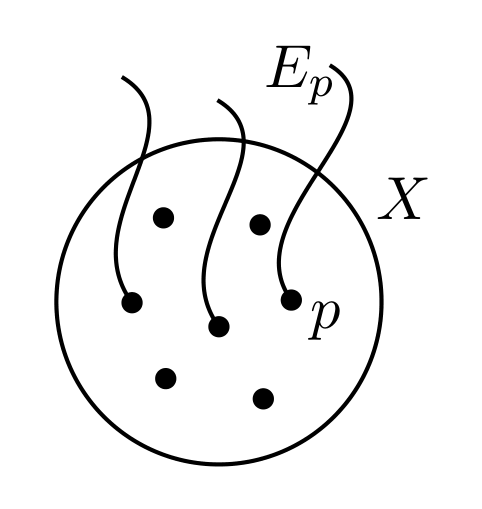
\includegraphics[width=0.22\linewidth]{fig_p004_1.png}
  \caption*{示意图：底流形 $X$、点 $p$ 及其上的纤维 $E_p$；场空间
    $\mathcal{E}=\Gamma(X,E)$ 是丛 $E\to X$ 的截面空间（原文 PDF p.4，原文无编号）}
\end{figure}

% [Tutor Note: 第二个要点中 $\mathcal{E}\neq\prod_{p\in X}E_p$ 的“不等”是关键：
% 截面空间 $\Gamma(X,E)$ 是乘积的子空间（要求截面在 $X$ 上连续/光滑地拼接），
% 不是逐点纤维的任意选择。原作者用“$\neq$”强调这一点，而不是说两者毫无关系。
% 这也解释了为何 $X$ 的拓扑会影响可观测量代数——局域截面如何粘合是拓扑问题。]

粗略地说，\emph{可观测量}是场上的函数，记为 $\mathcal{O}(\mathcal{E})$。例如，分布是线性可观测量。新的结构来自以下事实。给定开子集 $U\subset X$，我们可以谈论
支撑在 $U$ 中的可观测量 $\operatorname{Obs}(U)$：
\[
  \operatorname{Obs}(U)=\mathcal{E}(U)\ \text{上的函数}=\Gamma(U,E).
\]

% [Tutor Note: 这里已隐含了“层”的观点：$U\mapsto\operatorname{Obs}(U)$ 是一个
% 预层，限制映射由场的限制 $\mathcal{E}(V)\to\mathcal{E}(U)$ 对偶给出。第 8 章
% 把这一结构公理化为预因子化代数（prefactorization algebra）：不只是限制，
% 还要求互不相交开集上的可观测量可以“相乘”。]

\begin{wexam}{1.1}
  $\mathcal{E}=C^{\infty}(X)$，$p\in X$。考虑
  \[
    \begin{aligned}
      \mathcal{O}_1:\ \mathcal{E}&\longrightarrow \R,\\
      f&\longmapsto \mathcal{O}_1(f)=f(p)^3.
    \end{aligned}
  \]
  $\mathcal{O}_1$ 是一个支撑在 $p$ 的任意开邻域中的可观测量。
\end{wexam}

给定包含在开集 $V$ 中的互不相交开子集 $U_i\subset V$，使得其不交并
$\bigsqcup_i U_i\subset V$，我们对可观测量有一个映射（\emph{因子化乘积}）：
\[
  \bigotimes_i \operatorname{Obs}(U_i)\longrightarrow \operatorname{Obs}(V).
\]
直观上，如果把 $\mathcal{E}(U)$ 限制到 $\mathcal{E}(U_i)$，则对偶地有
$\mathcal{O}(\mathcal{E}(U_i))\to\mathcal{O}(\mathcal{E}(U))$。朴素地，我们可以把
这些函数\emph{相乘}，于是得到
\[
  \bigotimes_i \operatorname{Obs}(U_i)\longrightarrow \operatorname{Obs}(V).
\]
然而，这需要进一步的\emph{量子修正}，因为 $U_i$ 中的场可能相互“交谈”。这一代数结构在物理中称为\emph{算子乘积展开}（operator product expansion, OPE），在数学中
称为\emph{因子化乘积}（factorization product）。QFT 中可观测量代数的这种数学理论
在以下工作中得到发展：

\begin{itemize}[leftmargin=1.6em,itemsep=0.2em]
  \item Beilinson--Drinfeld \textup{[5]}：发展了\emph{因子化代数}，用以表述二维
        手征共形场论（CFT），并引入了\emph{手征同调}（chiral homology）的概念。
  \item Costello--Gwilliam \textup{[11]}：在 Batalin--Vilkovisky（BV）形式
        \textup{[3]} 下，由微扰重整化理论构造了因子化代数。
\end{itemize}

% >>> p005
\begin{wexam}{1.2}（拓扑量子力学（TQM））
  在拓扑 QFT 中，$\operatorname{Obs}(U)$ 只依赖于 $U$ 的拓扑。考虑 $\dim X=1$
  （一维 QFT 就是量子力学），且对任意可缩开区间 $U$ 有 $\operatorname{Obs}(U)=A$。
  现在考虑 $X$ 上的两个开区间 $U_1,U_2$，并把它们嵌入一个更大的区间 $V$ 之中。

  \begin{figure}[htbp]
    \centering
    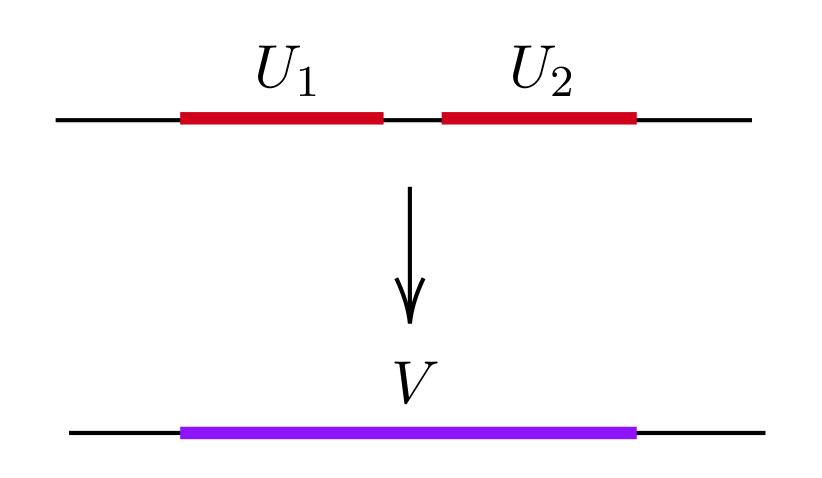
\includegraphics[width=0.33\linewidth]{fig_p005_1.png}
    \caption*{示意图：两个开区间 $U_1,U_2$ 嵌入更大的区间 $V$
      （原文 PDF p.5，原文无编号）}
  \end{figure}

  在拓扑理论中，因子化乘积不依赖于位置与大小。这给出一个映射
  \[
    \operatorname{Obs}(U_1)\otimes\operatorname{Obs}(U_2)\longrightarrow
    \operatorname{Obs}(V),
    \qquad\text{或}\qquad A\otimes A\longrightarrow A.
  \]
  我们得到一个\emph{结合代数}！我们还可以加入边界。

  \begin{figure}[htbp]
    \centering
    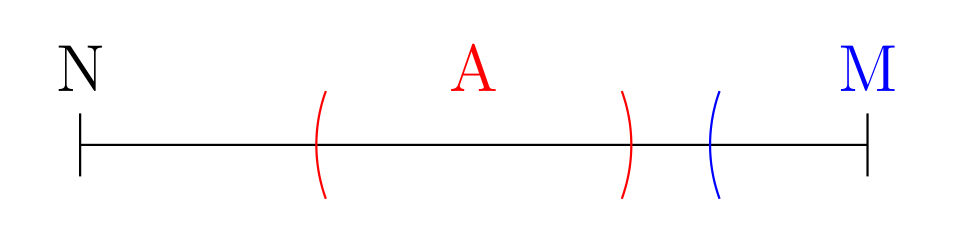
\includegraphics[width=0.38\linewidth]{fig_p005_2.png}
    \caption*{示意图：加入边界 $N,M$ 后，$A$ 的乘法给出 $A\otimes M\to M$ 与
      $N\otimes A\to N$（原文 PDF p.5，原文无编号）}
  \end{figure}

  于是得到 $A\otimes M\to M$，这意味着 $M$ 是一个左 $A$-模。类似地，$N$ 是一个
  右 $A$-模。总而言之，量子力学研究算子代数及其表示（模）。

  本例中出现的代数结构有如下的同调解释。考虑两个算子被放置在直线上的两个不同点。
  当一个算子靠近另一个时，直线拓扑的代数结构来自同调群
  \[
    H_{\bullet}(\R-\{0\})=H_0(\R-\{0\})=\Z_{\mathrm{left}}\oplus\Z_{\mathrm{right}},
  \]
  它由左乘与右乘构成。结合性来自进一步的一致性：

  \begin{figure}[htbp]
    \centering
    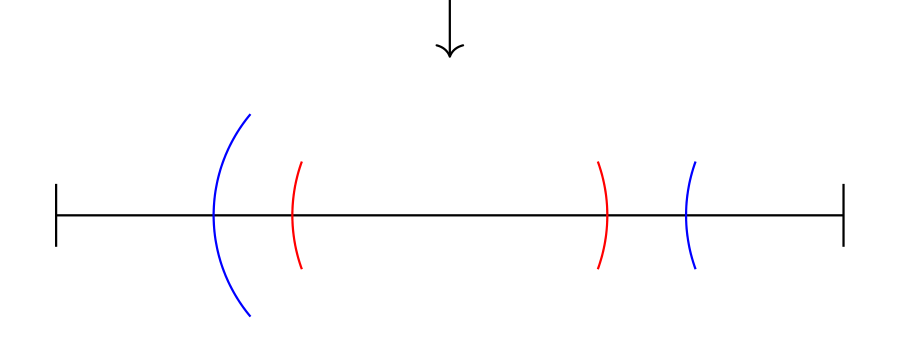
\includegraphics[width=0.36\linewidth]{fig_p005_3.png}
    \caption*{示意图：结合性 $(a\cdot b)\cdot c=a\cdot(b\cdot c)$ 的一致性条件
      （原文 PDF p.5，原文无编号）}
  \end{figure}

  \[
    \Longrightarrow\quad (a\cdot b)\cdot c=a\cdot(b\cdot c),
    \qquad a,b,c\in\operatorname{Obs}(U_i),\ i=1,2,3.
  \]
\end{wexam}

% [Tutor Note: $H_{\bullet}(\R-\{0\})=H_0(\R-\{0\})=\Z_{\mathrm{left}}\oplus
% \Z_{\mathrm{right}}$ 是启发性说明：直线上两个算子的构型空间有两个连通分支
% （左、右），分别对应左乘与右乘。严格的说法应把“算子放在点上”换成“区间嵌入的
% 余运算”（operad/因子化代数），见 Costello--Gwilliam [11] 第 1 卷。]

% >>> p006
\begin{wexam}{1.3}（二维手征 QFT）
  设 $\dim X=2$。二维（2d）手征理论的因子化乘积是全纯的。

  \begin{figure}[htbp]
    \centering
    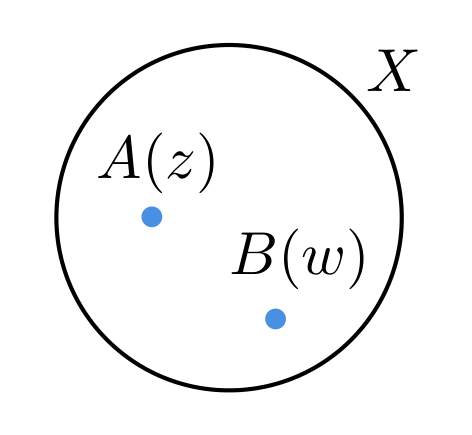
\includegraphics[width=0.22\linewidth]{fig_p006_1.png}
    \caption*{示意图：二维手征理论中算子 $A(z)$ 与 $B(w)$ 及其相互绕行
      （原文 PDF p.6，原文无编号）}
  \end{figure}

  在全纯坐标下，当一个算子靠近（或绕行）另一个算子时，绕数可以通过它们的
  Fourier/Laurent 模来表达：
  \[
    A(z)B(w)=\sum_{n\in\Z}\frac{(A_{(n)}B)(w)}{(z-w)^{n+1}}.
  \]
  我们得到无穷多个“乘积”（或二元运算）$\{A_{(n)}B\}$。此时可观测量代数给出一个
  \emph{顶点算子代数}（vertex operator algebra）。

  % [Tutor Note: OPE 的模记号 $(A_{(n)}B)(w)$ 与分母幂次 $(z-w)^{n+1}$ 是顶点代数
  % （Borcherds 意义）的标准约定；有些文献写成 $(z-w)^{-n-1}$ 并对 $n$ 作相反的
  % 编号，两者只差一个重编号。核对公式时先看分母幂次是 $n+1$ 还是 $-n-1$，
  % 这是极易出错处。]
\end{wexam}

% [Tutor Note: 原文 PDF p.6 作 "These examples play an fundamental role..."，
% 其中 "an" 应为 "a"，属原文笔误；p.3 的 "quanatum field theory" 亦应为
% "quantum field theory"。按体例照录原文意思、不擅自改写英文原文，仅在此注明。]

这些例子在引导我们理解量子场论中的一般构造方面起着根本性的作用，后文将会看到。


% ---------- part02.tex ----------
% ============================================================
%  part02.tex  |  原文 PDF p.7–14（页脚 p.6–13）
%  内容：第 2 章 上同调与积分
%        （2.1 de Rham 上同调；2.2 上同调与积分）
% ============================================================

% >>> p007
\section{上同调与积分（Cohomology and Integration）}

\begin{keypoints}
  \item \textbf{核心物理图像}：“积分”可以与上同调类配对来理解：闭形式沿闭链的积分
        只依赖于该链的同调类，这正是后文把路径积分视为“同调/上同调运算”的原型。
  \item \textbf{数学工具}：上链复形与上同调 $(C^{\bullet},d)$、de Rham 复形
        $(\Omega^{*}(U),d)$、Stokes 定理、Poincaré 引理，以及 Cartan 公式
        $\mathcal{L}_V=\dd\iota_V+\iota_V\dd$ 与内积 $\iota_V$。
  \item \textbf{主要结论}：Poincaré 引理给出 $H^{p}(\R^n)=0\ (p>0)$ 而
        $H^{n}_{c}(\R^n)\cong\R$；由积分映射
        $\int_{\R^n}:H^{n}_{c}(\R^n)\to\R$ 可知“积分”本质上是一种同调运算
        （与紧支集上同调对偶）。
  \item \textbf{译者评注}：本章是全书的代数与几何预备。2.2 节末尾“积分
        $\Longleftrightarrow$ 上同调”的观点，是第 6、7 章在 BV 形式与微扰量子化中
        把路径积分当作同调运算处理的雏形；Poincaré 引理的证明则示范了 Cartan 公式
        的典型用法（构造同伦算子），建议与第 6 章的收缩同伦对照阅读。
\end{keypoints}

\subsection{de Rham 上同调（De Rham Cohomology）}

我们讨论“积分”的一些代数与几何侧面，这些内容将有助于我们理解后文的量子场论构造。

\begin{wdefn}{2.1}
  环 $R$ 上的一个\emph{上链复形}（cochain complex）是一列 $R$-模映射
  \[
    \cdots\longrightarrow C^{n-1}\xrightarrow{\ d_{n-1}\ }C^{n}
    \xrightarrow{\ d_{n}\ }C^{n+1}\longrightarrow\cdots
  \]
  使得 $d_{n}d_{n+1}=0$。我们将其记为 $(C^{\bullet},d)$，其中
  $d_{n}=d|_{C^{n}}$ 且 $d^{2}=0$。
\end{wdefn}

% [Tutor Note: 原文 Definition 2.1 中条件印作 $d_nd_{n+1}=0$，但紧接下文用它推出
% $\mathrm{Im}(d_{n-1})\subset\mathrm{Ker}(d_n)$，而上链复形的相邻映射是
% $d_{n-1}:C^{n-1}\to C^n$ 与 $d_n:C^n\to C^{n+1}$，故该条件按复合次序应写作
% $d_n\circ d_{n-1}=0$（等价地 $d^2=0$）。此处照录原文，读者按 $d^2=0$ 理解即可。]

条件 $d_{n}d_{n+1}=0$ 蕴涵
\[
  \operatorname{Im}(d_{n-1})\subset\operatorname{Ker}(d_{n}).
\]
于是我们可以定义 $R$-模
\[
  H^{n}(C^{*},d):=\frac{\operatorname{Ker}(d_{n})}{\operatorname{Im}(d_{n-1})},
\]
它称为 $(C^{*},d)$ 的\emph{第 $n$ 个上同调群}。这是链复形与同调群的对偶概念。

% [Tutor Note: 原文上标记号不统一：p.6 用 $(C^{\bullet},d)$（实心圆点）表示上链
% 复形，随后又写 $H^{n}(C^{*},d)$、$(\Omega^{*}(U),d)$（星号），而 p.13 的命题
% 2.11 又回到 $\Omega^{\bullet}(U)$；同理 p.7 的 Definition 2.2 把 de Rham 上同调
% 写成 $H_{dR}^{P}(U)=H^{P}(\Omega^{*},d)$（大写 $P$），而紧随其后又写
% $H^{p}(M)$、$H_{c}^{p}(M)$（小写 $p$）。这些都是原文记号不一致，并非排版笔误；
% 本译本按原页照录，读者理解为同一复形、同一上标 $p$ 即可。]

\paragraph{de Rham 复形（De Rham Complex）}

下面考虑微积分中的一个几何例子。设 $U\subset\R^n$ 是开集，
$\{x^{1},\ldots,x^{n}\}$ 是它的坐标。引入
\[
  \begin{aligned}
    \Omega^{0}(U)&=\{\text{$U$ 上的光滑函数}\}=C^{\infty}(U),\\
    \Omega^{1}(U)&=\{\text{$U$ 上的光滑 $1$-形式}\}.
  \end{aligned}
\]
元素 $\alpha\in\Omega^{1}(U)$ 可以写成
\[
  \alpha=\sum_{i=1}^{n}\alpha_{i}(x)\dd x^{i}\in\Omega^{1}(U),
  \qquad \alpha_{i}\in C^{\infty}(U).
\]
全微分给出一个映射
\[
  \begin{aligned}
    \Omega^{0}(U)&\xrightarrow{\ \dd\ }\Omega^{1}(U)\\
    f&\longmapsto \dd f=\sum_{i}\partial_{i}f\,\dd x^{i},
  \end{aligned}
\]
它可以延拓为一个上链复形
\[
  \Omega^{0}(U)\xrightarrow{\ \dd\ }\Omega^{1}(U)\xrightarrow{\ \dd\ }
  \Omega^{2}(U)\to\cdots\xrightarrow{\ \dd\ }\Omega^{n}(U),
\]
其中
\[
  \Omega^{p}(U)=\{\text{$U$ 上的光滑 $p$-形式}\}.
\]
元素 $\xi\in\Omega^{p}(U)$ 形如
\[
  \xi=\sum_{i_{1},\ldots,i_{p}}\xi_{i_{1}\cdots i_{p}}(x)\,
  \dd x^{i_{1}}\wedge\cdots\wedge\dd x^{i_{p}}.
\]

% >>> p008
其中 $\xi_{i_{1}\cdots i_{p}}(x)\in C^{\infty}(U)$，并满足反对称性质
\[
  \dd x^{i}\wedge\dd x^{j}=-\dd x^{j}\wedge\dd x^{i},\qquad \forall i,j.
\]
特别地，$\dd x^{i}\wedge\dd x^{i}=0$。因此我们也可以写成
\[
  \Omega^{p}(U)=\bigoplus_{1\le i_{1}<\cdots<i_{p}\le n}
  C^{\infty}(U)\,\dd x^{i_{1}}\wedge\cdots\wedge\dd x^{i_{p}}.
\]
de Rham 微分 $d:\Omega^{p}(U)\to\Omega^{p+1}(U)$ 定义为
\[
  \dd(\xi)=\sum_{i_{1},\ldots,i_{p},k}
  \partial_{x^{k}}\xi_{i_{1}\cdots i_{p}}\,
  \dd x^{k}\wedge\dd x^{i_{1}}\wedge\cdots\wedge\dd x^{i_{p}}.
\]
验证：$d^{2}=0$。因此
\[
  \Omega^{0}(U)\xrightarrow{\ \dd\ }\Omega^{1}(U)\xrightarrow{\ \dd\ }
  \Omega^{2}(U)\to\cdots\to\Omega^{n}(U)
\]
定义了一个上链复形，称为 \emph{de Rham 复形}，记为 $(\Omega^{*}(U),d)$。

% [Tutor Note: 指标约定提醒——分解式中指标按 $1\le i_1<\cdots<i_p\le n$ 严格递增
% 求和，故每个基元只出现一次；若改用无序的 $i_1,\ldots,i_p$ 求和再反对称化，则与
% 上式相差一个 $p!$ 因子。这是微分形式计算中最常见的系数错误来源之一。]

\begin{wdefn}{2.2}
  $p$-形式 $\alpha\in\Omega^{p}$ 称为
  \begin{itemize}[leftmargin=1.6em,itemsep=0.12em,topsep=0.2em]
    \item \emph{闭的}（closed），若 $d\alpha=0$；
    \item \emph{恰当的}（exact），若 $\alpha=d\beta$ 对某个 $p-1$ 形式 $\beta$ 成立。
  \end{itemize}
  商空间
  \[
    H^{P}_{dR}(U)=H^{P}(\Omega^{*},d)
    =\frac{\text{闭的 }p\text{-形式}}{\text{恰当的 }p\text{-形式}}
  \]
  称为\emph{第 $p$ 个 de Rham 上同调}。
\end{wdefn}

de Rham 微分 $d$ 的一个重要性质是它是\emph{内蕴的}：它不依赖于坐标的选取。
因此我们可以通过粘接上述局部构造，在光滑流形 $M$ 上定义 $(\Omega^{*}(M),d)$。
于是流形上的 de Rham 上同调
\[
  H^{p}(M)=H^{p}_{dR}(M)
\]
是良定义的。我们也可以考虑 $(\Omega^{*}_{c}(M),d)$，其中
\[
  \Omega^{*}_{c}(M)=\{\text{$M$ 上具紧支集的 }p\text{-形式}\}.
\]
于是可以定义\emph{紧支集 de Rham 上同调}
\[
  H^{p}_{c}(M)=H^{p}(\Omega^{*}_{c}(M),d).
\]

\paragraph{Stokes 定理（Stokes' Theorem）}

设 $\mathcal{K}\subset\R^{n}$ 是一个 $p$ 维曲面，$\partial\mathcal{K}$ 是
$\mathcal{K}$ 的边界。$\mathcal{K}$ 的定向按下述方式决定 $\partial\mathcal{K}$ 的
一个定向。设 $x\in\mathcal{K}$，$\vec{n}_{x}$ 是 $\partial\mathcal{K}$ 上的一个
外法向量场，即 $\vec{n}_{x}$ 在 $\mathcal{K}$ 处相切，并指向 $\mathcal{K}$ 的外部。

% >>> p009
\begin{figure}[htbp]
  \centering
  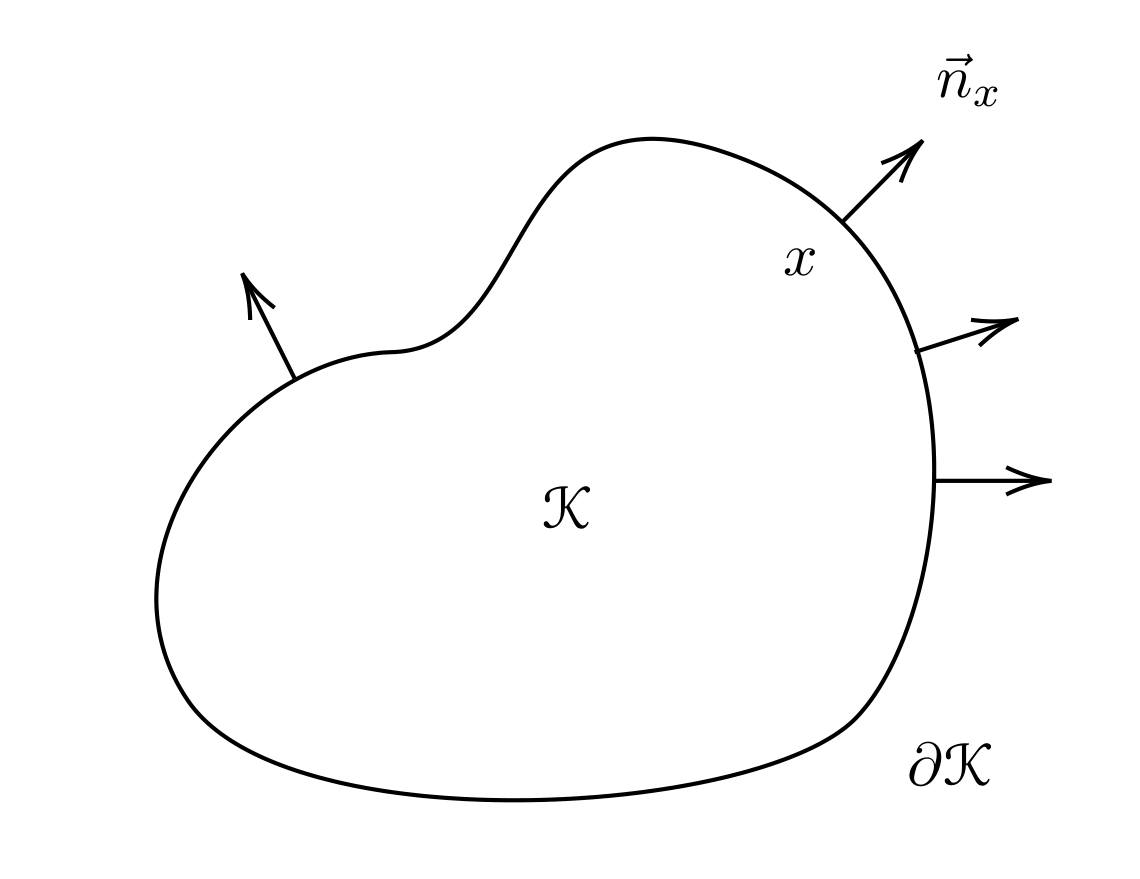
\includegraphics[width=0.46\linewidth]{fig_p009_1.png}
  \caption*{曲面 $\mathcal{K}$、其边界 $\partial\mathcal{K}$ 与外法向量 $\vec{n}_x$（原文 PDF p.9 示意图，原文无编号）}
\end{figure}

于是 $\partial\mathcal{K}$ 的一个定向参数化 $\tau^{1},\cdots,\tau^{p-1}$
满足：$\vec{n}_{x},\frac{\partial}{\partial\tau^{1}},\cdots,
\frac{\partial}{\partial\tau^{p-1}}$ 给出 $T_{x}\mathcal{K}$ 的一个定向。
按此诱导定向，我们有

% [Tutor Note: 原文 "$\vec{n}_x$ is tangent at $\mathcal{K}$" 的说法含糊：外法向量
% 应是 $\partial\mathcal{K}$ 的外法向（垂直于 $\partial\mathcal{K}$），而非
% $\mathcal{K}$ 的切向量。这里作者想说的是“$\vec{n}_x$ 附着在（沿）$\mathcal{K}$
% 的边界上”。按原文照录，读者按“外法向”理解即可。]

\begin{wthm}{2.3}（Stokes 定理）
  \[
    \int_{\mathcal{K}}\dd\alpha=\int_{\partial\mathcal{K}}\alpha.
  \]
  这里 $\alpha$ 是一个光滑的 $(p-1)$-形式。
\end{wthm}

% [Tutor Note: 边界诱导定向的约定（把外法向 $\vec n_x$ 放在参数化切向量之前）
% 直接决定 Stokes 公式的符号。Green 定理取 $n=p=2$、Gauss 定理取 $n=p=3$，
% 两例中 $\dd\alpha$ 展开式前面的正负号都依赖这一约定；核对符号时请先确认
% “外法向在前”还是“切向量在前”。这是本章最易出符号错误的地方。]

\begin{wexam}{2.4}
  考虑 $n=p=2$ 的情形。令
  \[
    \alpha=\alpha_{1}(x)\dd x^{1}+\alpha_{2}(x)\dd x^{2},
    \qquad
    \dd\alpha=\left(\frac{\partial\alpha_{2}}{\partial x^{1}}
    -\frac{\partial\alpha_{1}}{\partial x^{2}}\right)\dd x^{1}\wedge\dd x^{2}.
  \]
  于是
  \[
    \iint_{\mathcal{K}}\left(\frac{\partial\alpha_{2}}{\partial x^{1}}
    -\frac{\partial\alpha_{1}}{\partial x^{2}}\right)\dd x^{1}\wedge\dd x^{2}
    =\int_{\partial\mathcal{K}}\alpha_{1}(x)\dd x^{1}+\alpha_{2}(x)\dd x^{2}.
  \]
  这给出 Green 定理。
\end{wexam}

\begin{wexam}{2.5}
  考虑 $n=p=3$ 的情形。令
  \[
    \alpha=\alpha_{1}(x)\dd x^{2}\wedge\dd x^{3}
    +\alpha_{2}(x)\dd x^{3}\wedge\dd x^{1}
    +\alpha_{3}(x)\dd x^{1}\wedge\dd x^{2}.
  \]
  \[
    \dd\alpha=\left(\frac{\partial\alpha_{1}}{\partial x^{1}}
    +\frac{\partial\alpha_{2}}{\partial x^{2}}
    +\frac{\partial\alpha_{3}}{\partial x^{3}}\right)
    \dd x^{1}\wedge\dd x^{2}\wedge\dd x^{3}.
  \]
  于是
  \[
    \begin{aligned}
      &\iiint_{K}\left(\frac{\partial\alpha_{1}}{\partial x^{1}}
        +\frac{\partial\alpha_{2}}{\partial x^{2}}
        +\frac{\partial\alpha_{3}}{\partial x^{3}}\right)
        \dd x^{1}\wedge\dd x^{2}\wedge\dd x^{3}\\
      &\qquad=\iint_{\partial\mathcal{K}}\alpha_{1}(x)\dd x^{2}\wedge\dd x^{3}
        +\alpha_{2}(x)\dd x^{3}\wedge\dd x^{1}
        +\alpha_{3}(x)\dd x^{1}\wedge\dd x^{2}.
    \end{aligned}
  \]
  这就是 Gauss 积分定理。
\end{wexam}

% [Tutor Note: 例 2.5 中三重积分的下标原文作正体的 $K$（$\iiint_K$），而右边
% 二重积分的下标作花体 $\partial\mathcal{K}$（$\iint_{\partial\mathcal{K}}$）；
% 例 2.4 中则统一用花体 $\mathcal{K}$。这是原文同一页内的记号不一致，照录不改。]

作为 Stokes 定理的一个应用，考虑两个区域 $\mathcal{K}_{1}$ 与 $\mathcal{K}_{2}$，
它们作为下方图形所示区域 $\mathcal{M}$ 的边界。
\[
  \partial\mathcal{M}=\mathcal{K}_{2}-\mathcal{K}_{1}.
\]
这里的 $\pm$ 号由定向决定。

\begin{figure}[htbp]
  \centering
  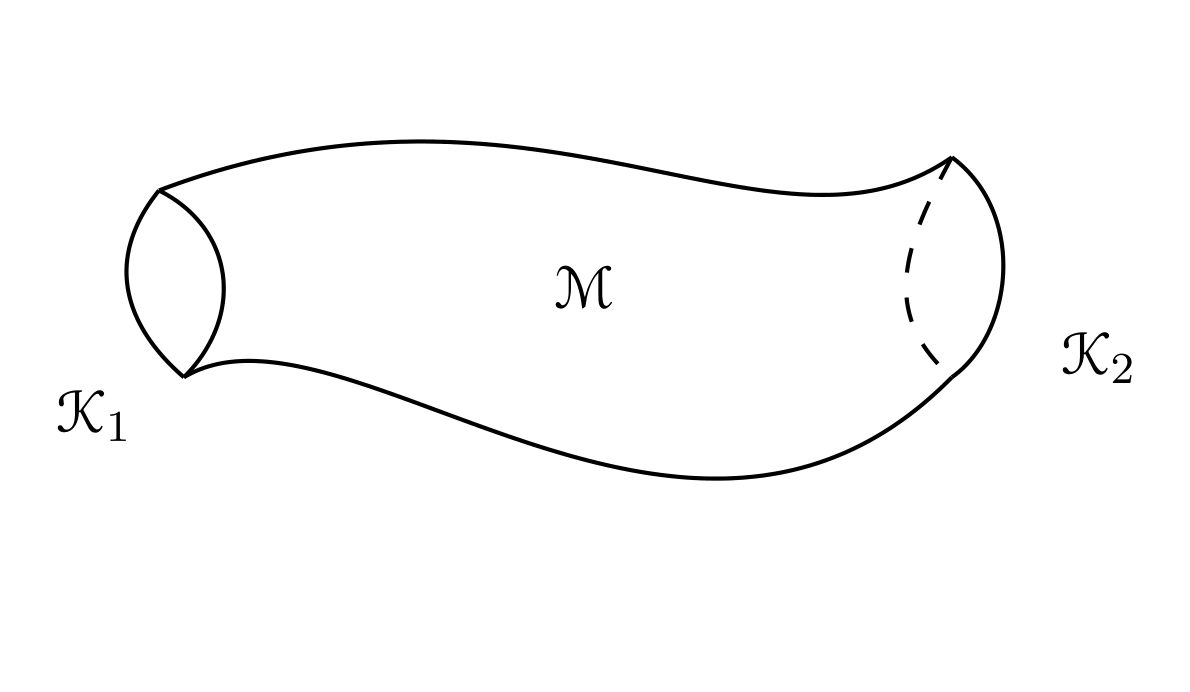
\includegraphics[width=0.48\linewidth]{fig_p009_2.png}
  \caption*{区域 $\mathcal{M}$ 及其边界 $\mathcal{K}_1$、$\mathcal{K}_2$（原文 PDF p.9 示意图，原文无编号）}
\end{figure}

% >>> p010
设 $\alpha$ 是一个闭形式
\[
  \dd\alpha=0.
\]
则
\[
  \int_{\mathcal{K}_{2}}\alpha-\int_{\mathcal{K}_{1}}\alpha
  =\int_{\partial\mathcal{M}}\alpha=\int_{\mathcal{M}}\dd\alpha=0.
\]
所以
\[
  \int_{\mathcal{K}_{1}}\alpha=\int_{\mathcal{K}_{2}}\alpha.
\]
特别地，若 $d\alpha=0$，则 $\int_{\mathcal{K}}\alpha$ 在 $\mathcal{K}$ 的
任何光滑形变下保持不变。

% [Tutor Note: “any smooth deformation”应理解为保持边界（更一般地，保持同调类）
% 的形变/同伦；若形变过程中扫过的区域包含奇点或使曲面穿过“洞”，积分可能改变，
% 例 2.7 正是这种反例。严格表述见 de Rham 定理：闭形式沿链的积分只依赖同调类。]

\begin{wexam}{2.6}
  设 $\alpha\in\Omega^{1}(\R^{n})$ 且 $\dd\alpha=0$。设 $p,q\in\R^{n}$ 是两点。
  定义
  \[
    \int_{p}^{q}\alpha=\int_{\gamma}\alpha
  \]
  其中 $\gamma$ 是连接 $p$ 与 $q$ 的任一条光滑路径。它不依赖于 $\gamma$ 的选取，
  因为任一条这样的路径 $\gamma_{1}$ 都可以连续形变为另一条 $\gamma_{2}$。于是由
  Stokes 定理，
  \[
    \int_{\gamma_{1}}\alpha=\int_{\gamma_{2}}\alpha.
  \]
\end{wexam}

\begin{figure}[htbp]
  \centering
  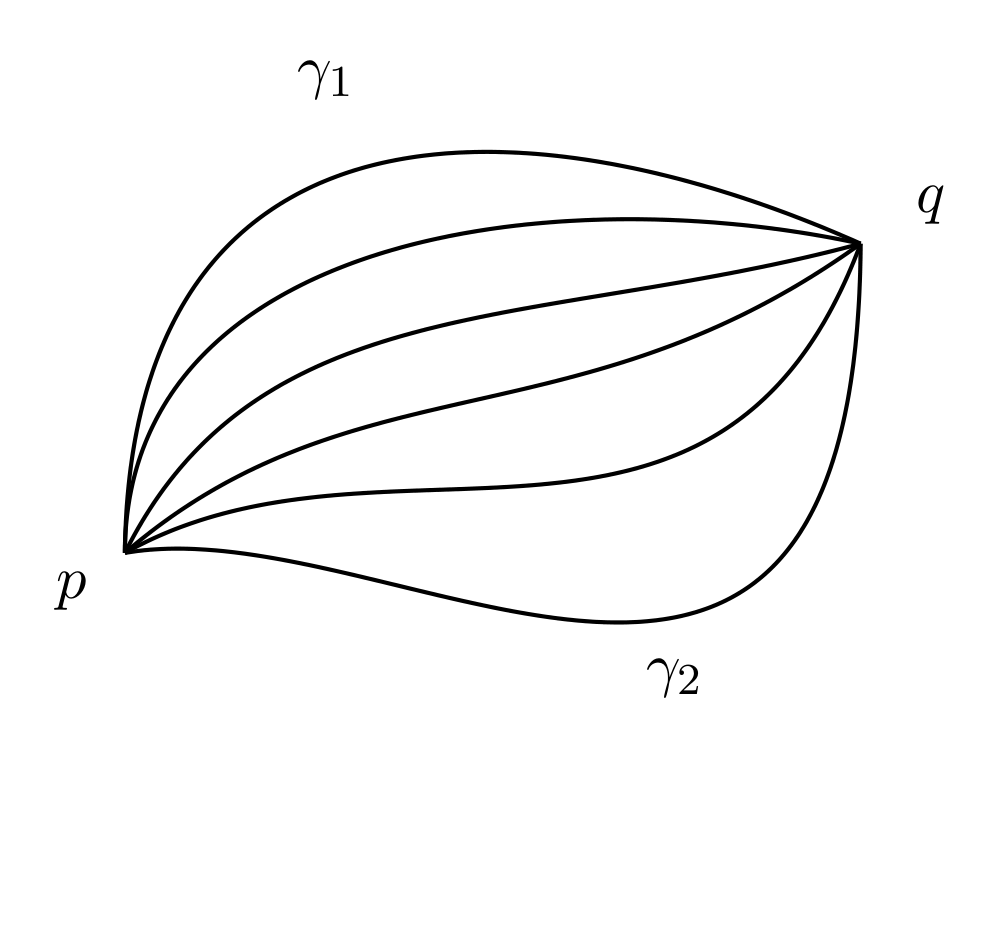
\includegraphics[width=0.40\linewidth]{fig_p010_1.png}
  \caption*{连接 $p$ 与 $q$ 的一族路径 $\gamma_1$、$\gamma_2$（原文 PDF p.10 示意图，原文无编号）}
\end{figure}

\begin{wexam}{2.7}
  考虑 $\mathcal{U}=\R^{2}-\{0\}$ 以及
  \[
    \alpha=\frac{x\,\dd y-y\,\dd x}{x^{2}+y^{2}},
    \qquad \dd\alpha=0.
  \]
  我们考虑从 $p=-1$ 到 $q=1$ 的两条路径，分别沿上半圆与下半圆。
\end{wexam}

\begin{figure}[htbp]
  \centering
  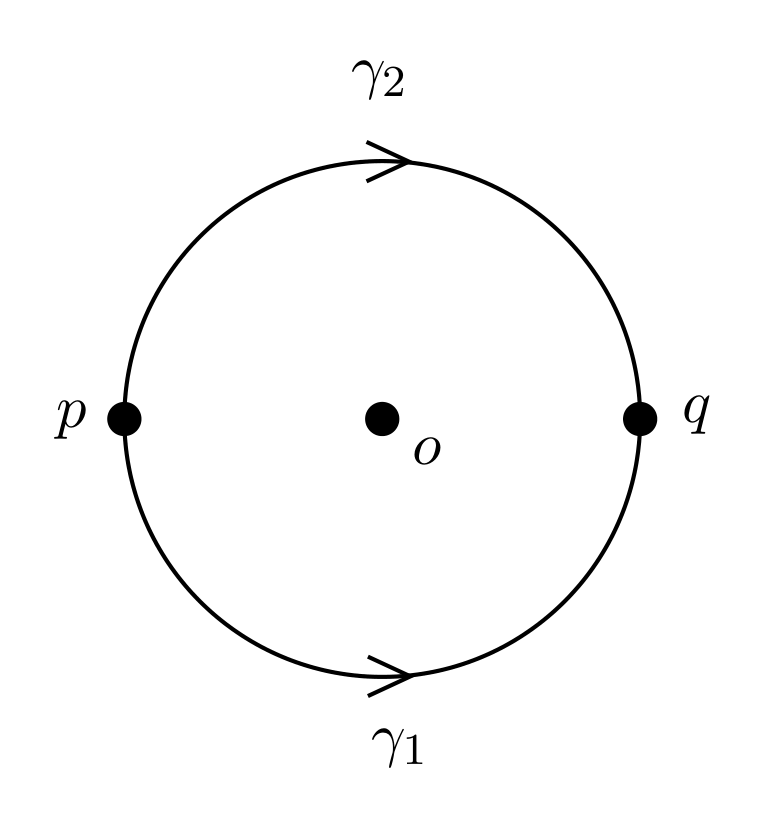
\includegraphics[width=0.31\linewidth]{fig_p010_2.png}
  \caption*{绕原点的上、下半圆路径 $\gamma_2$、$\gamma_1$（原文 PDF p.10 示意图，原文无编号）}
\end{figure}

% [Tutor Note: 本例是 $H^{1}_{dR}(\R^{2}-\{0\})\cong\R$ 的标准生成元：$\alpha$ 在
% $\mathcal{U}$ 上闭而不恰当。关键点是极坐标下 $\alpha=\dd\theta$，而 $\theta$
% 在 $\mathcal{U}$ 上并非单值函数，故不能写成某个整体函数的微分。判断“闭而不恰当”
% 时，务必先确认区域是否有洞（拓扑障碍），否则容易误判。]

% >>> p011
由于中间有一个洞，$\gamma_{1}$ 无法在区域 $\mathcal{U}$ 内形变为 $\gamma_{2}$。
这也可以通过计算看出：
\[
  \int_{\gamma_{1}}\alpha-\int_{\gamma_{2}}\alpha=\oint_{C}\alpha.
\]

\begin{figure}[htbp]
  \centering
  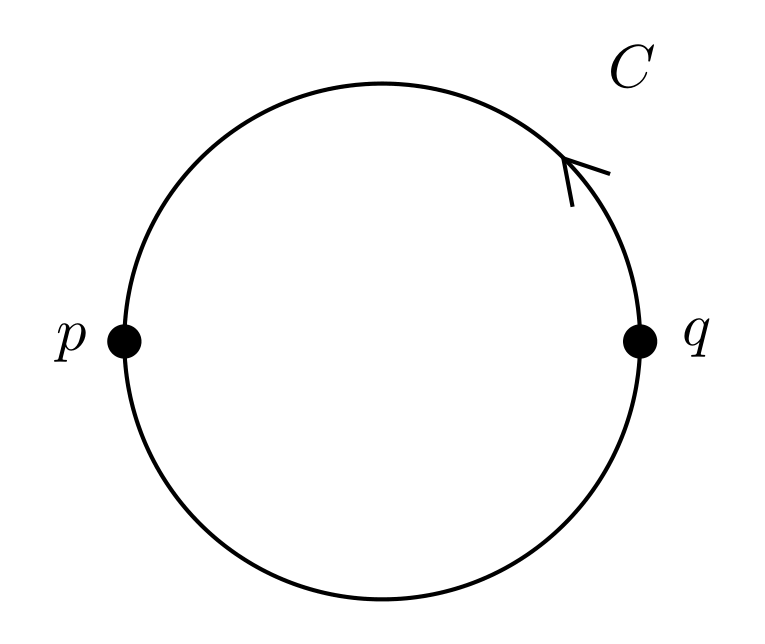
\includegraphics[width=0.31\linewidth]{fig_p011_1.png}
  \caption*{环绕洞的闭曲线 C（原文 PDF p.11 示意图，原文无编号）}
\end{figure}

用极坐标 $x=r\cos\theta$，$y=r\sin\theta$，
\[
  \alpha=\dd\theta,\qquad
  \oint_{C}\alpha=\int_{0}^{2\pi}\dd\theta=2\pi\ne 0.
\]

% [Tutor Note: 这里 $\oint_C\alpha=2\pi$ 是绕数（winding number）为 $1$ 的直接
% 体现；若把 $C$ 换成绕原点 $k$ 圈的闭曲线，积分给出 $2k\pi$，这正是
% $H^{1}_{dR}(\R^{2}-\{0\})\cong\R$ 的“周期”实现。原文此处的不等号印作
% $2\pi\neq 0$，本译本照录。]

\subsection{上同调与积分（Cohomology v.s. Integration）}

\begin{wthm}{2.8}（Poincaré 引理）
  \[
    H^{p}(\R^{n})=
    \begin{cases}
      \R, & p=0\\
      0,  & p>0
    \end{cases},
    \qquad
    H^{p}_{c}(\R^{n})=
    \begin{cases}
      \R, & p=n\\
      0,  & p\ne n
    \end{cases}
  \]
  $H^{0}(\R^{n})$ 的一个生成元是常函数 $f\equiv 1$。$H^{n}_{c}(\R^{n})$ 的一个
  生成元是一个紧支集形式 $\alpha=f(x)\dd^{n}x$，其中 $f\in C^{\infty}_{c}(\R^{n})$，
  且满足 $\int_{\R^{n}}\alpha=1$。
\end{wthm}

观察到任意 $n$-形式 $\alpha\in\Omega^{n}_{c}(\R^{n})$ 都是闭的。另一方面，若
$\alpha=\dd\beta$，其中 $\beta\in\Omega^{n-1}_{c}(\R^{n})$，则
\[
  \int_{\R^{n}}\dd\beta=\int_{K}\dd\beta=\int_{\partial K}\beta=0,
\]
其中 $K$ 是一个足够大的球。积分映射
\[
  \begin{aligned}
    \int_{\R^{n}}:\ H^{n}_{c}(\R^{n})&\longrightarrow\R\\
    \alpha&\longmapsto\int\alpha
  \end{aligned}
\]
正是 Poincaré 引理中所述的同构。换个角度看，映射
\[
  \begin{aligned}
    \Omega^{n}_{c}(\R^{n})&\longrightarrow H^{n}_{c}(\R^{n})
    \overset{\text{Poincaré}}{\cong}\R,\\
    \alpha&\longmapsto[\alpha]
  \end{aligned}
\]
把最高次 $n$-形式送到它的上同调类，恰好确定了积分（相差一个重新标度的常数）。
因此
\[
  \int_{\R^{n}}\quad\Longleftrightarrow\quad H^{n}_{c},
\]
也就是说，“积分”可以用一种同调运算来刻画。这一观点在我们后文关于微扰量子化的
讨论中将起重要作用。

本小节的其余部分用于证明 Poincaré 引理。

% [Tutor Note: 这是本章的核心思想，也是全书的重要线索：积分不应只被看成“测度”，
% 而应看成上同调类之间的配对 $\int_{\R^n}\leftrightarrow H^{n}_{c}$。第 6、7 章
% 把路径积分 $\int_{\mathcal{E}}\ee^{\ii S/\hbar}(-)$ 解释为 BV 形式下的同调/上同调
% 运算（Costello 的因子化代数与微扰量子化），其思想源头正是这里。]

% >>> p012
\paragraph{Cartan 公式（Cartan Formula）}

我们先介绍微分几何中一些有用的概念。令
\[
  \Vect(M)=\text{流形 }M\text{ 上的光滑向量场}.
\]
向量场 $V\in\Vect(M)$ 可以按坐标表示为
\[
  V(x)=\sum_{i}V^{i}(x)\frac{\partial}{\partial x^{i}}.
\]
我们可以把 $V$ 看作一阶微分算子
\[
  \begin{aligned}
    V:\ C^{\infty}(M)&\to C^{\infty}(M)\\
    f&\mapsto V(f)=\sum_{i}V^{i}(x)\frac{\partial f}{\partial x^{i}},
  \end{aligned}
\]
它满足 Leibniz 法则（即定义一个导子）：
$V(fg)=V(f)g+fV(g)$。

$\Vect(M)$ 在括号下构成一个 Lie 代数
\[
  \begin{aligned}
    [-,-]:\ \Vect(M)\times\Vect(M)&\longrightarrow\Vect(M)\\
    (V,W)&\longmapsto[V,W].
  \end{aligned}
\]
这个括号满足以下性质：
\begin{itemize}[leftmargin=1.6em,itemsep=0.25em,topsep=0.2em]
  \item 作为微分算子
        \[
          [V,W](f):=V(W(f))-W(V(f)).
        \]
  \item 用坐标显式写出
        \[
          [V,W]=\sum_{i}\left(V(W^{i})-W(V^{i})\right)
          \frac{\partial}{\partial x^{i}}.
        \]
  \item Jacobi 恒等式
        \[
          [V,[W,T]]+[W,[T,V]]+[T,[V,W]]=0.
        \]
\end{itemize}

% [Tutor Note: 坐标公式 $[V,W]=\sum_i\big(V(W^i)-W(V^i)\big)\partial_i$ 中，
% $V(W^i)$ 表示把 $V$ 作为方向导数作用在函数 $W^i$ 上，即
% $\sum_j V^j\partial_j W^i$，而不是 $V^iW^i$ 之类的分量乘积。这是初学时最常见的
% 混淆点；请与下一个 Jacobi 恒等式一起核对分量指标。]

我们可以把 $\Vect(M)$ 形式地看作 $M$ 的微分同胚群 $\Diff(M)$ 的 Lie 代数。
设 $V$ 在 $M$ 上生成一个流
\[
  \begin{aligned}
    \varphi:\ (-\varepsilon,\varepsilon)\times M&\longrightarrow M\\
    (t,x)&\longmapsto\varphi(t,x),
  \end{aligned}
\]
满足 $\varphi(0,x)=x$ 以及
$\frac{\partial\varphi(t,x)}{\partial t}=V(\varphi)$。记
\[
  \begin{aligned}
    \varphi_{t}:\ M&\longrightarrow M\\
    x&\longmapsto\varphi(t,x),
  \end{aligned}
\]
它满足群性质：$\varphi_{0}=\mathrm{Id}$，$\varphi_{t}\varphi_{s}=\varphi_{t+s}$，
$\varphi^{-1}=\varphi_{-t}$。于是
\[
  V(f)(x)=\left.\frac{\dd}{\dd t}\right|_{t=0}f(\varphi_{t}(x))
\]
表示 $f$ 沿 $V$ 所生成流的无穷小变化。

% [Tutor Note: 原文 “$\varphi^{-1}=\varphi_{-t}$” 的记法不严谨，应理解为
% $\varphi_t^{-1}=\varphi_{-t}$（对每个固定的 $t$，$\varphi_t$ 是 $M$ 的微分同胚，
% 其逆为 $\varphi_{-t}$）。按原文照录，特此注明。]

% >>> p013
这一整套形式可以推广到微分形式。回忆一个光滑映射
\[
  \begin{aligned}
    \phi:\ X&\longrightarrow Y\\
    x&\longmapsto y^{i}=\phi^{i}(x)
  \end{aligned}
\]
使我们能定义“拉回”（pull-back）映射
\[
  \phi^{*}:\ \Omega^{p}(Y)\longrightarrow\Omega^{p}(X),
\]
它把 $\alpha=\sum\alpha_{i_{1}\cdots i_{p}}(y)\dd y^{i_{1}}\wedge\cdots
\wedge\dd y^{i_{p}}$ 送到
\[
  \phi^{*}(\alpha)=\sum\alpha_{i_{1}\cdots i_{p}}(\phi(x))
  \dd\phi^{i_{1}}(x)\wedge\cdots\dd\phi^{i_{p}}(x).
\]
特别地，$V$ 生成的流 $\varphi_{t}$ 给出
\[
  \varphi_{t}^{*}:\ \Omega^{p}(M)\to\Omega^{p}(M).
\]

\begin{wdefn}{2.9}
  我们通过下式定义微分形式上的 \emph{Lie 导数} $\mathcal{L}_{V}$：
  \[
    \begin{aligned}
      \mathcal{L}_{V}:\ \Omega^{p}&\to\Omega^{p}\\
      \alpha&\mapsto\mathcal{L}_{V}(\alpha):=
      \left.\frac{\dd}{\dd t}\right|_{t=0}\partial_{t}^{*}(\alpha).
    \end{aligned}
  \]
\end{wdefn}

% [Tutor Note: 原文 Definition 2.9 的第二式印作 $\partial_t^*(\alpha)$，但按上下文
% （对 $V$ 生成的流 $\varphi_t$ 的拉回求导），此处应为 $\varphi_t^*(\alpha)$；
% 疑为原文笔误（把 $\varphi$ 误排成 $\partial$）。本译本照录原文的
% $\partial_t^*(\alpha)$，请核对原书 p.12。]

另一方面，向量场与 $1$-形式之间的自然配对引出内积（interior product）的概念。

\begin{wdefn}{2.10}
  我们定义微分形式上的\emph{内积} $\iota_{V}$：
  \[
    \begin{aligned}
      \iota_{V}:\ \Omega^{p}&\to\Omega^{p-1}\\
      \alpha&\mapsto\iota_{V}\alpha
    \end{aligned}
  \]
  如下给出：
  \[
    \begin{aligned}
      \iota_{V}\big(\alpha_{i_{1}\cdots i_{p}}(x)\dd x^{i_{1}}\wedge\cdots
      \dd x^{i_{p}}\big)
      :={}&\sum\alpha_{i_{1}\cdots i_{p}}\iota_{V}(\dd x^{i_{1}})
      \wedge\cdots\wedge\dd x^{i_{p}}\\
      &-\sum\alpha_{i_{1}\cdots i_{p}}\dd x^{i_{1}}
      \wedge\iota_{V}(\dd x^{i_{2}})\wedge\cdots\wedge\dd x^{i_{p}}\\
      &+\cdots+(-1)^{p-1}\sum\alpha_{i_{1}\cdots i_{p}}\dd x^{i_{1}}
      \wedge\cdots\wedge\iota_{V}(\dd x^{i_{p}}).
    \end{aligned}
  \]
  这里对 $V=\sum_{i}V^{i}(x)\frac{\partial}{\partial x^{i}}$，有
  $\iota_{V}(\dd x^{i})=V^{i}(x)$。
\end{wdefn}

% [Tutor Note: 内积的第一行原文作 $\iota_V(\dd x^{i_1})\wedge\cdots\wedge\dd x^{i_p}$，
% 按标准展开式应为 $\iota_V(\dd x^{i_1})\wedge\dd x^{i_2}\wedge\cdots\wedge\dd x^{i_p}$
% （省略号中隐含 $\dd x^{i_2}$）；末项符号 $(-1)^{p-1}$ 与指标次序相关，逐项核对
% 指标时极易出错，建议用 $p=2,3$ 的小例子验算。]

现在我们有三个算子
\[
  \begin{aligned}
    d&:\ \Omega^{p}\to\Omega^{p+1}\\
    \mathcal{L}_{V}&:\ \Omega^{p}\to\Omega^{p}\\
    \iota_{V}&:\ \Omega^{p}\to\Omega^{p-1}.
  \end{aligned}
\]
它们之间由 \emph{Cartan 魔法公式}（Cartan's Magic Formula）相联系：
\[
  \mathcal{L}_{V}=d\iota_{V}+\iota_{V}d.
\]
上述关系还可以进一步推广如下。

\begin{wprop}{2.11}
  设 $V,W\in\Vect(U)$。则作为 $\Omega^{\bullet}(U)$ 上的算子，
  \begin{itemize}[leftmargin=1.6em,itemsep=0.25em,topsep=0.2em]
    \item $[\mathcal{L}_{V},\mathcal{L}_{W}]
          :=\mathcal{L}_{V}\mathcal{L}_{W}-\mathcal{L}_{W}\mathcal{L}_{V}
          =\mathcal{L}_{[V,W]}$。
    \item $\iota_{V}\iota_{W}+\iota_{W}\iota_{V}=0$。
    % >>> p014
    \item $[\mathcal{L}_{V},d]:=\mathcal{L}_{V}d-d\mathcal{L}_{V}=0$。
    \item $\iota_{V}d+d\iota_{V}=\mathcal{L}_{V}$。
    \item $[\mathcal{L}_{V},\iota_{W}]
          :=\mathcal{L}_{V}\iota_{W}-\iota_{W}\mathcal{L}_{V}
          =\iota_{[V,W]}$。
  \end{itemize}
\end{wprop}

\begin{proof}[Poincaré 引理的证明]
  我们证明 $H^{p}(\R^{n})$ 的情形，紧支集的情形留给读者。考虑微分同胚
  \[
    \begin{aligned}
      \varphi_{t}:\ \R^{n}&\longrightarrow\R^{n}\\
      (x^{1},\ldots,x^{n})&\longmapsto(e^{t}x^{1},\ldots,e^{t}x^{n}),
    \end{aligned}
  \]
  它是向量场 $V=\sum x^{i}\frac{\partial}{\partial x^{i}}$ 生成的流。注意
  $\varphi_{0}=\mathrm{Id}$，而 $\varphi_{-\infty}$ 是常值映射
  \[
    \varphi_{-\infty}:\ \R^{n}\longrightarrow\{0\}\in\R^{n}.
  \]
  设 $p>0$，并设 $\alpha\in\Omega^{p}(\R^{n})$ 是闭形式：$d\alpha=0$。由于
  \[
    \varphi_{0}^{*}(\alpha)=\alpha,\qquad
    \varphi_{-\infty}^{*}(\alpha)=0,
  \]
  我们有
  \[
    \begin{aligned}
      \alpha&=\varphi_{0}^{*}(\alpha)-\varphi_{-\infty}^{*}(\alpha)\\
      &=\int_{-\infty}^{0}\frac{\dd}{\dd t}\big(\varphi_{t}^{*}(\alpha)\big)\dd t\\
      &=\int_{-\infty}^{0}\mathcal{L}_{V}\big(\varphi_{t}^{*}(\alpha)\big)\dd t\\
      &=\int_{-\infty}^{0}(d\iota_{V}+\iota_{V}d)\big(\varphi_{t}^{*}(\alpha)\big)\dd t.
    \end{aligned}
  \]
  这里我们用了 Cartan 公式。

  由于 $\alpha$ 闭，$d\varphi_{t}^{*}(\alpha)=\varphi_{t}^{*}(d\alpha)=0$，
  于是可以进一步化简为
  \[
    \alpha=d\left(\int_{-\infty}^{0}\iota_{V}\big(\varphi_{t}^{*}(\alpha)\big)
    \dd t\right)=d\beta,
  \]
  其中 $\beta=\int_{-\infty}^{0}\iota_{V}\big(\varphi_{t}^{*}(\alpha)\big)\dd t$。
  这说明当 $p>0$ 时 $H^{p}(\R^{n})=0$。对 $p=0$，
  \[
    f\in H^{0}(\R^{n})\quad\Longrightarrow\quad \dd f=0
    \quad\Longrightarrow\quad f=\mathrm{const}.
  \]
  因此 $H^{0}(\R^{n})=\R$。
\end{proof}

% [Tutor Note: 本证明中有三处原文排印问题（照录并在正文中按可读形式复原）：
% (i) $\varphi_{-\infty}:\R^n\to\{0\}\in\R^n$ 中的 “$\in$” 应为 “$\subset$”
% （常值映射的像为单点集 $\{0\}\subset\R^n$）；(ii) 原文 “$H^p(\R^n)=0$ for
% $p>0..$” 末尾多一个句点，(iii) 原文的 $\alpha=d\big(\int\iota_V(\varphi_t^*(\alpha)
% \dd t)\big)$ 少一个右括号且 $\dd t$ 落在 $\iota_V$ 括号内；本译本按下一行 $\beta$
% 的定义式（$\dd t$ 在 $\iota_V$ 之外）复原为
% $\alpha=d\big(\int\iota_V(\varphi_t^*(\alpha))\dd t\big)$。三点均请核对原书 p.13。]


% ---------- part03.tex ----------
% ============================================================
%  part03.tex  |  原文 PDF p.15–22（页脚 p.14–21）
%  内容：第 3 章 经典场论
%        （3.1 运动方程；3.2 Noether 定理；3.3 规范对称性）
% ============================================================

% >>> p015
\section{经典场论（Classical Field Theory）}

\begin{keypoints}
  \item \textbf{核心物理图像}：经典场论由作用量泛函 $S:\mathcal{E}\to\R/\C$ 描述；
        经典解即作用量的临界点（运动方程），而连续对称性对应守恒流与守恒荷。
  \item \textbf{数学工具}：向量丛截面与 jet、变分法与分部积分、Lie 群在无穷维场空间
        $\mathcal{E}$ 上的作用及其无穷小形式、微分形式的 Hodge 星算子与外微分。
  \item \textbf{主要结论}：Noether 定理的两种推导——“变分 $\delta^G_\varepsilon\mathcal{L}
        =\varepsilon^\alpha\dd\kappa_\alpha$”与“把 $\varepsilon$ 提升为函数 $\tilde\varepsilon(x)$
        再分部积分”；自发对称性破缺指经典解本身不保持该对称群；规范对称性是局域对称性，
        Maxwell 方程可统一写成 $\dd F=0$ 与 $\dd({*}F)={*}J$。
  \item \textbf{译者评注}：3.3 节用微分形式重写 Maxwell 理论，是全书后文以 BV/BRST
        处理规范对称性（第 6、7 章）的直接铺垫。Noether 流
        $J_\alpha=\gamma_\alpha-\kappa_\alpha$ 的构造依赖“分部积分产生 $\dd\gamma$”
        这一约定，$\kappa_\alpha$ 又只定义到 $\dd$-闭形式，读时需留意其不定性。
\end{keypoints}

\subsection{运动方程（Equation of Motion）}

考虑由作用量泛函 $S$ 描述的经典场论
\[
  S:\ \mathcal{E}\longrightarrow\R/\C.
\]
通常，$\mathcal{E}$ 将是流形 $X$ 上某个向量丛 $E$ 的光滑截面空间。我们假设 $X$ 是
$n$ 维且已定向的，则 $S$ 将是一个\emph{局部}泛函，其\emph{拉格朗日密度}
$\mathcal{L}$ 取值于 $X$ 上的 $n$-形式：
\[
  S[\phi]=\int_{X}\mathcal{L}(\phi),\qquad \phi\in\mathcal{E}.
\]
拉格朗日密度由 $\phi$ 的 jet 构造而成，即由 $\phi$ 及其各阶导数构造而成。

% [Tutor Note: 记号提醒——原文用花体 $\mathcal{E}$ 表示“场空间”，用直立体 $E$ 表示
% $X$ 上的向量丛，二者关系是 $\mathcal{E}=\Gamma(X,E)$（光滑截面空间）。同一句中
% 同时出现 “$\mathcal{E}$” 与 “a vector bundle $E$”，切勿混为一谈；这与第 1 章
% 的约定一致，本译本严格保留。]

\begin{wexam}{3.1}（相空间上的力学）
  在 Hamilton 力学中，我们可以用相空间 $\R^{2m}$ 上由时间 $t$ 参数化的路径来描述
  一个场
  \[
    \phi=\{q^{i}(t),p_{i}(t)\}:\ \R\longrightarrow\R^{2m}.
  \]
  于是场空间为
  \[
    \mathcal{E}=C^{\infty}(\R)^{\oplus 2m},
  \]
  它可以等同于位于 $X=\R$ 上的平凡丛的光滑截面空间。作用量 $S$ 由相空间上的
  Hamilton 函数 $H$ 构造：
  \[
    \begin{aligned}
      S[\phi]&=\int p_{i}\dd q^{i}-H(q,p)\dd t\\
      &=\int\left(p_{i}(t)\dot q^{i}(t)-H(q,p)\right)\dd t.
    \end{aligned}
  \]
  由于这里的路径是一维对象，我们可以把量子力学看作一维量子场论。
\end{wexam}

\begin{wexam}{3.2}（标量场论）
  设 $(X,g)$ 是 Riemann 流形，$\mathcal{E}$ 是光滑函数空间 $C^{\infty}(X)$。
  考虑作用量
  \[
    S[\phi]=\int_{X}\left(\frac{1}{2}|\nabla\phi|^{2}+V(\phi)\right)\dd Vol_{g},
  \]
  其中 $|\nabla\phi|^{2}=\partial_{i}\phi\partial_{j}\phi g^{ij}$，$V$ 是势函数，
  体积元为 $\dd Vol_{g}=\sqrt{g}\,\dd^{n}x$。假设 $X$ 没有边界，则我们也可以写成
  \[
    S[\phi]=\int_{X}\left(-\frac{1}{2}\phi\Delta\phi+V(\phi)\right)\dd Vol_{g},
  \]
  其中 $\Delta$ 是 \emph{Laplace--Beltrami 算子}（$-\Delta$ 是正算子）
  \[
    \Delta\phi=\frac{1}{\sqrt{g}}\partial_{i}\left(\sqrt{g}g^{ij}\partial_{j}\phi\right).
  \]
  对 $X=\R^{n}$ 及标准度规 $g=(\dd x^{1})^{2}+(\dd x^{2})^{2}+\cdots+(\dd x^{n})^{2}$，
  \[
    \Delta=\sum_{i}\frac{\partial^{2}}{\partial x^{i}\partial x^{i}}.
  \]
\end{wexam}

% [Tutor Note: 本例有两个易错点。(i) $|\nabla\phi|^{2}=\partial_i\phi\partial_j\phi g^{ij}$
% 中指标 $i,j$ 一上一下缩并，$g^{ij}$ 是度规逆矩阵的分量；若把 $g^{ij}$ 写成 $g_{ij}$
% 会得到错误的符号/数值。(ii) 从 $\int\frac12|\nabla\phi|^2$ 到 $-\int\frac12\phi\Delta\phi$
% 用了分部积分并丢掉了边界项——这正是原文假设 “$X$ has no boundary” 的用处；$\Delta$
% 的符号约定为 $\Delta=\frac{1}{\sqrt g}\partial_i(\sqrt g\,g^{ij}\partial_j)$，
% 故 $-\Delta$ 为正算子，Euclidean 情形下与通常的 $-\nabla^2$ 一致。]

% >>> p016
\begin{wexam}{3.3}（Chern--Simons 理论）
  设 $X$ 是一个三维流形，$\Lie{g}$ 是一个半单 Lie 代数，带有非退化的迹配对
  （Killing 型）$\Tr:\Lie{g}\otimes\Lie{g}\to\R$。为简单起见，考虑平凡丛，并令
  \[
    \mathcal{E}=\Omega^{1}(X,\Lie{g})
  \]
  是 $\Lie{g}$-值 $1$-形式的空间。Chern--Simons 作用量为
  \[
    CS[A]=\int_{X}\Tr\left(\frac{1}{2}A\wedge\dd A
    +\frac{1}{6}A\wedge[A,A]\right),\qquad A\in\mathcal{E},
  \]
  其中 $[-,-]$ 是由下式定义的广义 Lie 括号：
  \[
    [\alpha\otimes e_{1},\beta\otimes e_{2}]
    =(\alpha\wedge\beta)\otimes[e_{1},e_{2}],
    \qquad \text{对 } \alpha,\beta\in\Omega^{1}(X),\ e_{i}\in\Lie{g}.
  \]
\end{wexam}

\begin{wrem}{3.4}
  关于 Chern--Simons 的一般拓扑分类，见 \textup{[14]}。
\end{wrem}

在下面的讨论中我们假设 $X$ 没有边界。经典解是 $S$ 的临界点，
\[
  \Crit(S)=\{\delta S=0\}\subset\mathcal{E}.
\]
考虑任意的变分 $\delta\phi$。我们总可以用分部积分把作用量的变分写成
\[
  \delta S=\int_{X}EL(\phi)\delta\phi.
\]
由于 $\delta\phi$ 是任意的，我们得到经典运动方程
\[
  \Crit(S)=\{\phi:\ EL(\phi)=0\},
\]
它也称为 \emph{Euler--Lagrangian 方程}。

% [Tutor Note: “Euler--Lagrangian equation” 的通行名称是 Euler--Lagrange 方程
% （Euler–Lagrange equation）；原文用了 “Lagrangian”，属原文笔误，此处照录不擅改。
% 另注意 $EL(\phi)$ 是 Euler–Lagrange 导数（作为与 $\delta\phi$ 配对后积出 $n$-形式的
% 密度），与第 6 章 BV 形式中的 $\delta S/\delta\phi$ 是同一对象的不同记法。]

\begin{wexam}{3.5}（相空间上的力学）
  作用量泛函为
  \[
    S[q,p]=\int\left(p\dot q-H(q,p)\right)\dd t.
  \]
  其变分计算如下：
  \[
    \begin{aligned}
      \delta S&=\int\left[\delta p\,\dot q+p\frac{\dd}{\dd t}(\delta q)
      -\left(\frac{\partial H}{\partial q}\delta q
      +\frac{\partial H}{\partial p}\delta p\right)\right]\dd t\\
      &=\int\left(\dot q\delta p-\dot p\delta q
      -\frac{\partial H}{\partial q}\delta q
      -\frac{\partial H}{\partial p}\delta p\right)\dd t\\
      &=\int\left(\dot q-\frac{\partial H}{\partial p}\right)\delta p
      -\left(\dot p+\frac{\partial H}{\partial q}\right)\delta q.
    \end{aligned}
  \]
  经典运动方程是 \emph{Hamilton 方程}
  \[
    \begin{cases}
      \dot q=\dfrac{\partial H}{\partial p}\\[6pt]
      \dot p=-\dfrac{\partial H}{\partial q}.
    \end{cases}
  \]
\end{wexam}

% [Tutor Note: 例 3.5 变分的第三行原文末尾没有 $\dd t$（前两行都有），疑为排印遗漏；
% 此处照录原文。读时请自行补上 $\dd t$，否则 $\delta S$ 与 $\int(\cdots)$ 的量纲不匹配。
% 另外注意第一行 $\delta p\,\dot q$ 与 $p\frac{\dd}{\dd t}(\delta q)$ 来自
% $\delta(p\dot q)$，第二行对 $p\frac{\dd}{\dd t}(\delta q)$ 分部积分给出
% $-\dot p\,\delta q$（边界项已丢弃）。]

\begin{wexam}{3.6}（标量场论）
  \[
    S[\phi]=\int_{X}\left(\frac{1}{2}|\nabla\phi|^{2}+V(\phi)\right)\dd Vol_{g},
  \]
% >>> p017
  其变分给出
  \[
    \begin{aligned}
      \delta S&=\int_{X}\left(\nabla\phi\cdot\nabla\delta\phi
      +V'(\phi)\delta\phi\right)\dd Vol_{g}\\
      &=\int_{X}\left(-(\Delta\phi)\delta\phi+V'(\phi)\delta\phi\right)\dd Vol_{g}.
    \end{aligned}
  \]
  经典运动方程为
  \[
    -\Delta\phi+V'(\phi)=0.
  \]
\end{wexam}

\begin{wexam}{3.7}（Chern--Simons 理论）
  \[
    CS[A]=\int_{X}\Tr\left(\frac{1}{2}A\wedge\dd A
    +\frac{1}{6}A\wedge[A,A]\right).
  \]
  其变分给出
  \[
    \begin{aligned}
      \delta CS&=\int_{X}\Tr\left(\delta A\wedge\dd A
      +\frac{1}{2}\delta A\wedge[A,A]\right)\\
      &=\int_{X}\Tr\left(\delta A\wedge F_{A}\right),
    \end{aligned}
  \]
  其中 $F_{A}=\dd A+\frac{1}{2}[A,A]$ 是 $A$ 的曲率。经典运动方程
  \[
    F_{A}=0
  \]
  描述平坦联络。
\end{wexam}

\subsection{Noether 定理（Noether's Theorem）}

\paragraph{对称性（Symmetry）}

假设我们有一个经典理论
\[
  S:\ \mathcal{E}\longrightarrow\R/\C.
\]
所谓（经典）\emph{对称性}，是指一个群 $G$ 作用在 $\mathcal{E}$ 上，使得 $S$ 是
$G$-不变的：
\[
  S[g(\phi)]=S[\phi]\qquad \forall g\in G.
\]
经典对称性有两类：离散群对应的\emph{离散对称性}，以及 Lie 群对应的
\emph{连续对称性}。

\begin{wexam}{3.8}
  考虑相空间上作用量为
  \[
    S[q,p]=\int\left(p\dot q-H(q,p)\right)\dd t
  \]
  的力学。这里 Hamilton 函数 $H$ 不依赖于时间。存在 Lie 群 $\R$ 在 $\mathcal{E}$ 上
  由时间平移给出的光滑作用。对 $a\in\R$，定义 $\phi_{a}:\mathcal{E}\to\mathcal{E}$ 为
  \[
    \{q(t),p(t)\}\longmapsto\{q(t+a),p(t+a)\}.
  \]
  对任意 $a\in\R$，$S$ 在 $\phi_{a}$ 下不变。这给出一个连续对称性。

  考虑一个特定的 Hamilton 函数
  \[
    H(q,p)=\frac{1}{2}p^{2}+V(q),
  \]
  其中 $V$ 是偶函数。于是我们有一个离散的 $\Z_{2}$-对称性。记 $\sigma$ 为
  $\Z_{2}$ 的生成元，则该对称性由
  \[
    \sigma:(q,p)\to(-q,-p)
  \]
  给出。
\end{wexam}

% >>> p018
\paragraph{经典 Noether 定理（Classical Noether's Theorem）}

假设我们有一个由连通 Lie 群 $G$ 给出的连续对称性，其 Lie 代数为 $\Lie{g}$。
设无穷小变换取如下形式
\[
  \delta^{G}_{\varepsilon}\phi=\varepsilon^{\alpha}\mathcal{X}_{\alpha}(\phi),
\]
其中无穷小常数 $\varepsilon^{\alpha}$ 参数化 $\Lie{g}$ 中的元素。

% [Tutor Note: 这里 $\alpha$ 是 Lie 代数 $\Lie{g}$ 的指标，$\varepsilon^\alpha$ 与
% $\mathcal{X}_\alpha$ 按 Einstein 约定缩并；$\mathcal{X}_\alpha$ 是场空间
% $\mathcal{E}$ 上的向量场（即沿 $\mathcal{X}_\alpha$ 的无穷小变形），而不是底流形
% $X$ 上的向量场。第 2 章的向量场作用在 $X$ 上，这里的 $\mathcal{X}_\alpha$ 作用在
% 无穷维的 $\mathcal{E}$ 上，两者不可混淆。]

\begin{wexam}{3.9}
  时间平移的无穷小变换为
  \[
    \delta_{\varepsilon}\phi=\phi(t+\varepsilon)-\phi(t)=\varepsilon\dot\phi(t),
  \]
  且 $\mathcal{X}(\phi)=\dot\phi$。
\end{wexam}

设 $X$ 是 $n$ 维定向流形，且 $X$ 上有一个拉格朗日密度
\[
  S=\int_{X}\mathcal{L}(\phi).
\]
$S$ 的 $G$-不变性可以在无穷小层面表述为
\[
  \delta^{G}_{\varepsilon}\mathcal{L}=\varepsilon^{\alpha}\dd\kappa_{\alpha},
\]
其中 $\kappa_{\alpha}$ 是 $(n-1)$-形式。注意 $\kappa_{\alpha}$ 只在相差一个
$\dd$-闭形式的意义下定义。

另一方面，对任意变分
\[
  \delta\mathcal{L}=EL(\phi)\delta\phi+\dd\gamma,
\]
其中 $\dd\gamma$ 是分部积分产生的恰当 $n$-形式。代入由对称性给出的特殊变分
$\delta^{G}_{\varepsilon}$，我们可以写成
\[
  \begin{aligned}
    \delta^{G}_{\varepsilon}\mathcal{L}
    &=EL(\phi)\,\varepsilon^{\alpha}\mathcal{X}_{\alpha}(\phi)
    +\dd(\varepsilon^{\alpha}\gamma_{\alpha})\\
    &=\varepsilon^{\alpha}\left(EL(\phi)\,\mathcal{X}(\phi)
    +\dd\gamma_{\alpha}\right),
  \end{aligned}
\]
其中 $\gamma_{\alpha}$ 是由 $\gamma$ 与 $\mathcal{X}_{\alpha}$ 决定的某个量。
比较上面关于 $\delta^{G}_{\varepsilon}\mathcal{L}$ 的两个表达式，我们得到
\[
  \varepsilon^{\alpha}\left(\dd(\gamma_{\alpha}-\kappa_{\alpha})
  +EL(\phi)\,\mathcal{X}_{\alpha}(\phi)\right)=0.
\]
由于 $\varepsilon^{\alpha}$ 是任意的，我们得到
\[
  \dd J_{\alpha}+EL\,\mathcal{X}=0,
  \qquad\text{其中 } J_{\alpha}=\gamma_{\alpha}-\kappa_{\alpha}.
\]
特别地，在满足运动方程 $EL(\phi)=0$ 的构型处，
\[
  \dd J_{\alpha}\big|_{\Crit(S)}=0.
\]

% [Tutor Note: $\dd J_\alpha+EL\,\mathcal{X}=0$ 中的 $EL\,\mathcal{X}$ 是
% $EL(\phi)\mathcal{X}_\alpha(\phi)$ 的简写（原文照录），这是一个\emph{离壳}
% （off-shell）恒等式；限制到 $\Crit(S)$ 上才得到 $\dd J_\alpha=0$。$\kappa_\alpha$
% 只定义到 $\dd$-闭形式、$\gamma_\alpha$ 的选取又依赖分部积分的方式，因此
% $J_\alpha$ 只定义到 $\dd$-闭形式——这不影响守恒荷的守恒性，但比较不同文献的
% Noether 流时必须先固定这一约定。]

$J_{\alpha}$ 按下述方式给出守恒量。设 $Y_{1},Y_{2}\subset X$ 是两个由 $\Sigma$
同调起来的余维 $1$ 超曲面。Stokes 定理蕴涵：对 $\phi\in\Crit(S)$，
\[
  \int_{Y_{1}}J_{\alpha}(\phi)-\int_{Y_{2}}J_{\alpha}(\phi)
  =\int_{\partial\Sigma}J_{\alpha}
  =\int_{\Sigma}\dd J_{\alpha}=0.
\]
特别地，若 $X$ 是时空、$Y_{t}$ 是时刻 $t$ 的时间切片，则积分
$\int_{Y_{t}}J_{\alpha}$ 不依赖于 $t$（假设 $\phi$ 满足运动方程）。
$J_{\alpha}$ 称为\emph{守恒流}，而空间积分 $\int_{Y_{t}}J_{\alpha}$ 称为
\emph{守恒荷}。

上述论证表明：连续对称性对应于守恒流。这就是 Noether 定理的内容。

% >>> p019
\begin{figure}[htbp]
  \centering
  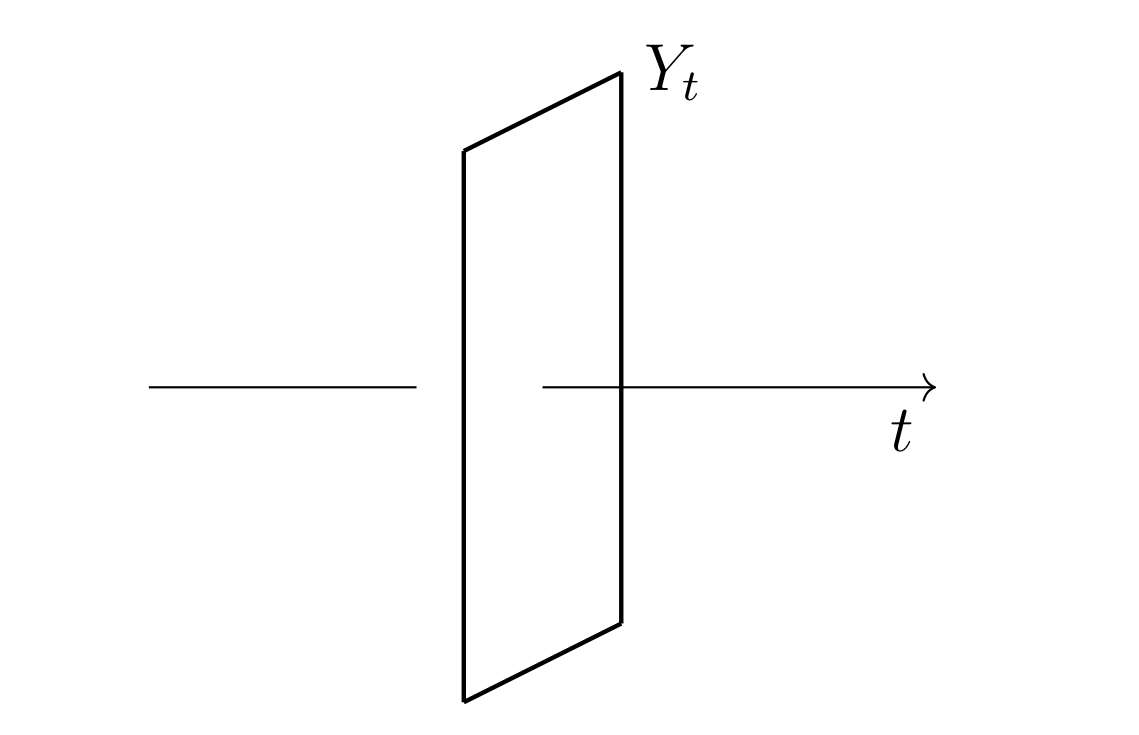
\includegraphics[width=0.46\linewidth]{fig_p019_1.png}
  \caption*{时空与时间切片 $Y_t$（原文 PDF p.19 示意图，原文无编号）}
\end{figure}

\begin{wexam}{3.10}
  考虑相空间上的力学
  \[
    S=\int\left(p\dot q-H(q,p)\right)\dd t.
  \]
  $S$ 的变分计算结果为
  \[
    \delta\mathcal{L}=(\dot q-\partial_{p}H)\delta p
    -(\dot p+\partial_{q}H)\delta q
    +\frac{\dd}{\dd t}(p\delta q).
  \]
  对无穷小时间平移
  \[
    \delta_{\varepsilon}q=\varepsilon\dot q,\qquad
    \delta_{\varepsilon}p=\varepsilon\dot p,
  \]
  我们有
  \[
    \delta_{\varepsilon}\mathcal{L}
    =\varepsilon\frac{\dd}{\dd t}\mathcal{L}.
  \]
  用上面的记号，我们得到
  \[
    \gamma=p\dot q,\qquad \kappa=\mathcal{L}.
  \]
  Noether 定理断言
  \[
    J=\gamma-\kappa=p\dot q-\mathcal{L}=H
  \]
  在 Hamilton 方程下守恒。这一事实可以直接验证：
  \[
    \frac{\dd}{\dd t}H=\partial_{p}H\,\dot p+\partial_{q}\dot q
    =-\partial_{p}H\,\partial_{q}H+\partial_{q}H\,\partial_{p}H=0.
  \]
  我们得到结论：时间平移对称性蕴涵能量守恒。
\end{wexam}

% [Tutor Note: 上面 $\frac{\dd}{\dd t}H=\partial_pH\,\dot p+\partial_q\dot q$
% 中第二项原文印作 $\partial_q\dot q$，按推导应为 $\partial_qH\,\dot q$
% （末式 $-\partial_pH\partial_qH+\partial_qH\partial_pH=0$ 也印证了这一点）；
% 疑为原文漏排 $H$，此处照录并注明，请核对原书 p.18。]

还有另一种等价的方式推导守恒流。我们将常数 $\varepsilon^{\alpha}$ 提升为 $X$ 上的
函数 $\tilde\varepsilon^{\alpha}(x)$，并考虑变分
\[
  \delta^{G}_{\tilde\varepsilon}\phi
  =\tilde\varepsilon^{\alpha}(x)\mathcal{X}_{a}(\phi).
\]
利用分部积分与 $S$ 的 $G$-不变性，我们总可以写成
\[
  \delta^{G}_{\tilde\varepsilon}S
  =-\int\tilde\varepsilon^{\alpha}\dd\tilde J_{\alpha},
\]
当 $\tilde\varepsilon^{\alpha}=\varepsilon^{\alpha}$ 为常数时它为零。

在运动方程上，对任意变分 $\delta\phi$ 都有 $\delta S=0$。把它作用于特殊变分
$\delta^{G}_{\tilde\varepsilon}\phi$，并利用 $\tilde\varepsilon(x)$ 的任意性，我们得到
$\dd\tilde J_{\alpha}=0$（在运动方程上）。这就是 Noether 流。

与前面的计算比较并利用 $\dd J_{\alpha}+EL\,\mathcal{X}=0$，
\[
  \delta^{G}_{\tilde\varepsilon}S
  =\int EL\,\delta^{G}_{\tilde\varepsilon}\phi
  =\int\tilde\varepsilon^{\alpha}EL\,\mathcal{X}_{\alpha}
  =-\int\tilde\varepsilon^{\alpha}\dd J_{\alpha}.
\]
因此 $J_{\alpha}=\tilde J_{\alpha}$ 模 $\dd$-闭形式。

% [Tutor Note: 原文在 $\delta^{G}_{\tilde\varepsilon}\phi
% =\tilde\varepsilon^{\alpha}(x)\mathcal{X}_{a}(\phi)$ 中把下标写成 $a$，
% 而同一段与上下文的无穷小变换写作 $\mathcal{X}_{\alpha}$；结合 Lie 代数指标
% $\alpha$ 的缩并方式，$a$ 疑为 $\alpha$ 的排印之误。此处照录 $\mathcal{X}_a$
% 并注明，请核对原书 p.18。]

% >>> p020
\begin{wexam}{3.11}
  我们用第二种方法计算作用量
  \[
    S=\int\left(p\dot q-H(q,p)\right)\dd t
  \]
  的时间平移。提升后的无穷小变换为
  \[
    \delta_{\tilde\varepsilon}\phi=\tilde\varepsilon\dot\phi.
  \]
  代入变分，得
  \[
    \delta_{\tilde\varepsilon}S
    =\int\tilde\varepsilon\frac{\dd}{\dd t}\mathcal{L}
    +\dot{\tilde\varepsilon}\,p\dot q
    =-\int\tilde\varepsilon\frac{\dd}{\dd t}(p\dot q-\mathcal{L})
    =\int\tilde\varepsilon\frac{\dd}{\dd t}H.
  \]
  我们再次得到 $\tilde J=H$。
\end{wexam}

% [Tutor Note: 例 3.11 最后一个等号的符号疑有误：由
% $-\int\tilde\varepsilon\frac{\dd}{\dd t}(p\dot q-\mathcal{L})$ 且
% $H=p\dot q-\mathcal{L}$，应得 $-\int\tilde\varepsilon\frac{\dd}{\dd t}H$；原文印作
% $+\int\tilde\varepsilon\frac{\dd}{\dd t}H$。若取原文的正号，则与
% $\delta_{\tilde\varepsilon}S=-\int\tilde\varepsilon\dd\tilde J$ 比较会得到
% $\tilde J=-H$，与下一句 “$\tilde J=H$” 矛盾。此处照录原文，请核对原书 p.19。]

\paragraph{自发对称性破缺（Spontaneous Symmetry Breaking）}

假设 $G$ 是一个对称性，则 $G$ 作用在经典解的空间上。然而，给定经典解
$\phi\in\Crit(S)$，$\phi$ 本身可能不被 $G$ 固定。在这种情况下，我们说该对称性是
\emph{自发破缺}的。

\begin{wexam}{3.12}
  考虑
  \[
    S=\int(p\dot q-H)\dd t,\qquad H=\frac{1}{2}p^{2}+V(q),
  \]
  其中 $V(q)=V(-q)$。我们有一个 $\Z_{2}$-对称性。运动方程为
  \[
    \begin{cases}
      \dot q=\dfrac{\partial H}{\partial p}=p\\[6pt]
      \dot p=-\dfrac{\partial H}{\partial q}=-V'(q).
    \end{cases}
  \]
  假设 $V'(a)=0$。则路径
  \[
    \begin{cases}
      q(t)=a\\
      p(t)=0
    \end{cases}
  \]
  是运动方程的解，但不被 $\Z_{2}$ 保持。
\end{wexam}

\begin{figure}[htbp]
  \centering
  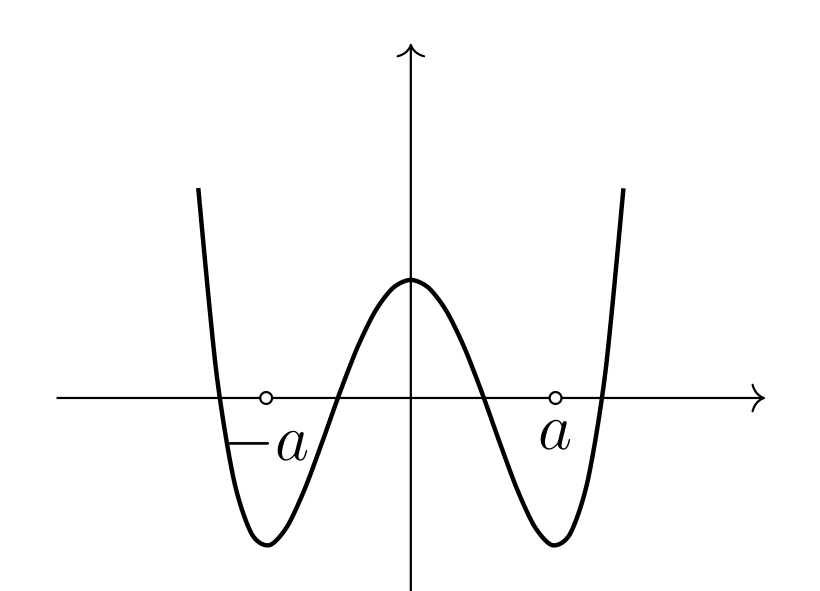
\includegraphics[width=0.33\linewidth]{fig_p020_1.png}
  \caption*{自发对称性破缺（原文 Figure 1，原文 p.19 / PDF p.20）}
\end{figure}

% [Tutor Note: Figure 1 是原文唯一的编号图（页脚 p.19 / PDF p.20），题注为
% “Spontaneous Symmetry Breaking”。图意是：势 $V(q)$ 为偶函数，两个极小点
% $q=\pm a$ 满足 $V'(a)=0$；经典解 $q(t)=a$、$p(t)=0$ 只选了其中一个极小，
% 从而破坏了 $\Z_2$ 对称性。注意“破缺”指的是\emph{解}不保持对称性，
% 作用量本身仍然是对称的——这是自发对称性破缺与明显破缺的根本区别。]

% >>> p021
\subsection{规范对称性（Gauge Symmetry）}

规范对称性是由\emph{局域}变换给出的对称性。设 $X$ 是时空流形。粗略地说，这里的
局域性是指：无穷小规范变换的集合构成一个 $C^{\infty}(X)$-模。规范变换的概念由
H. Weyl 引入。

\begin{wexam}{3.13}（Maxwell 方程）
  \[
    \begin{cases}
      \nabla\cdot\vec E=\dfrac{1}{\eps_{0}}\rho\\[6pt]
      \nabla\cdot\vec B=0\\[6pt]
      \nabla\times\vec E=-\dfrac{\partial\vec B}{\partial t}\\[6pt]
      \nabla\times\vec B=\mu_{0}\left(\vec j
      +\eps_{0}\dfrac{\partial\vec E}{\partial t}\right),
    \end{cases}
  \]
  其中 $\vec E=(E_{x},E_{y},E_{z})$ 与 $\vec B=(B_{x},B_{y},B_{z})$ 是电场与磁场，
  而 $\vec j=(j_{x},j_{y},j_{z})$ 是电流密度。在 $\R^{3,1}$ 上引入 $2$-形式
  \[
    F=(E_{x}\dd x+E_{y}\dd y+E_{z}\dd z)\wedge\dd t
    +B_{x}\dd y\wedge\dd z+B_{y}\dd z\wedge\dd x+B_{z}\dd x\wedge\dd y
  \]
  以及 $1$-形式
  \[
    J=\frac{1}{\eps_{0}}\rho\,\dd t
    -\mu_{0}(j_{x}\dd x+j_{y}\dd y+j_{z}\dd z).
  \]
  则 Maxwell 方程可以紧凑地改写为
  \[
    \begin{cases}
      \dd F=0\\
      \dd({*}F)={*}J,
    \end{cases}
  \]
  其中
  \[
    {*}:\ \Omega^{p}(\R^{3,1})\longrightarrow\Omega^{4-p}(\R^{3,1})
  \]
  是关于 Minkowski 度规的 Hodge 星算子。相容性条件 $\dd({*}J)=0$ 恰好就是
  电荷守恒。

  在可缩空间 $\R^{3,1}$ 上，$\dd F=0$ 蕴涵存在势 $1$-形式 $A$ 使 $F=\dd A$，
  它可以分解为标量势与矢量势：
  \[
    A=-\phi\,\dd t+\vec A
    =-\phi\,\dd t+A_{x}\dd x+A_{y}\dd y+A_{z}\dd z.
  \]
  于是我们可以把 Maxwell 方程改写为
  \[
    \begin{cases}
      \vec E=-\nabla\phi-\partial_{t}\vec A\\[6pt]
      \vec B=\nabla\times\vec A.
    \end{cases}
  \]
  规范变换由一个任意的 $0$-形式 $\chi$ 参数化，它把 $A$ 变为 $A+\dd\chi$，
  并保持 $F=\dd A$ 不变。

  引入作用量泛函
  \[
    S[A]=\frac{1}{\mu_{0}}\int_{\R^{3,1}}
    \left(\frac{1}{2}F\wedge{*}F+{*}J\wedge A\right).
  \]
  在变分 $A\to A+\delta A$ 下，
  \[
    \begin{aligned}
      \delta S&=\frac{1}{\mu_{0}}\int_{\R^{3,1}}
      \delta F\wedge{*}F+{*}J\wedge\delta A\\
      &=\frac{1}{\mu_{0}}\int_{\R^{3,1}}
      \dd\delta A\wedge{*}F-\delta A\wedge{*}J\\
      &=\frac{1}{\mu_{0}}\int_{\R^{3,1}}
      \delta A\wedge\left(\dd({*}F)-{*}J\right).
    \end{aligned}
  \]
\end{wexam}

% [Tutor Note: 这里 $F$ 的定义
% $F=(E_x\dd x+E_y\dd y+E_z\dd z)\wedge\dd t+B_x\dd y\wedge\dd z+\cdots$
% 依赖 Minkowski 度规的号差约定（原文取 $\R^{3,1}$，即 $(+,-,-,-)$ 型）。
% 换成 $(-,+,+,+)$ 号差时电场项的符号会改变；Hodge 星算子 ${*}$ 也随号差改变
% （${*}^2$ 在 4 维的 Lorentz 号差下满足 ${*}^2=-1$ 而非 $+1$）。对照其他文献的
% Maxwell 方程时，务必先确认号差与 $F$ 的约定，这是最容易出符号错误的地方。]

% [Tutor Note: 作用量 $S[A]$ 中两项的符号与系数 $(1/\mu_0)$ 是原文的约定；若采用
% SI 制之外的 Gauss 单位制，$\eps_0,\mu_0$ 会被吸收进场与电流的定义中。另注意
% ${*}J$ 是 $3$-形式（4 维中 Hodge 星把 $1$-形式映为 $3$-形式），故
% ${*}J\wedge A$ 与 $F\wedge{*}F$ 都是 $4$-形式，可以直接积分。]

% >>> p022
运动方程由下式读出：
\[
  \dd({*}F)-{*}J=0,
\]
它恰好就是 Maxwell 方程。

在规范变换 $A\to A+\dd\chi$ 下，
\[
  \delta_{\chi}S
  =\frac{1}{\mu_{0}}\int_{\R^{3,1}}{*}J\wedge\dd\chi
  =\frac{1}{\mu_{0}}\int_{\R^{3,1}}\dd({*}J)\wedge\chi=0.
\]
最后一个等号来自电荷守恒 $\dd({*}J)=0$。

% [Tutor Note: 这里的分部积分给出
% $\int{*}J\wedge\dd\chi=\int\dd({*}J)\wedge\chi$（无额外符号），因为
% ${*}J$ 是 $3$-形式、$\chi$ 是 $0$-形式，$\dd({*}J\wedge\chi)
% =\dd({*}J)\wedge\chi-{*}J\wedge\dd\chi$，边界项为零。若把被积式写成
% $J\wedge{*}\dd\chi$（而不是 ${*}J\wedge\dd\chi$），则会得到相反的符号；
% 规范化这一计算时需先固定 Hodge 星的作用位置。]


% ---------- part04.tex ----------
% ============================================================
%  part04.tex  |  原文 PDF p.23–30（页脚 p.22–29）
%  内容：第 4 章 对称性的代数方面（Algebraic Aspects of Symmetry）
%        4.1 Chevalley--Eilenberg 复形（PDF p.23–24）
%        4.2 微分分次 Lie 代数（DGLA）（PDF p.25–28）
%        4.3 同伦 Lie 代数（$L_\infty$-代数）（PDF p.29–30）
% ============================================================

% >>> p023
\section{对称性的代数方面（Algebraic Aspects of Symmetry）}

\begin{keypoints}
  \item \textbf{核心物理图像}：规范理论的代数骨架是“物质场 $+$ 鬼场 $+$ BRST 算子”构成的
        上链复形；经典对称性由 Lie 代数（更一般地，DGLA）描述，量子化之后其代数关系
        只在“同伦”意义下成立，这正是 $L_\infty$ 代数的由来。
  \item \textbf{数学工具}：外代数 $\bigwedge^{\bullet}\mathfrak g^{\vee}$、分次对称/反对称张量、
        Chevalley--Eilenberg 微分 $\dd_{\mathrm{CE}}$、微分分次 Lie 代数（DGLA）及其
        Chevalley--Eilenberg 复形、$L_\infty$ 代数。
  \item \textbf{主要结论}：$\dd_{\mathrm{CE}}^2=0$ 等价于 Lie 括号的 Jacobi 恒等式；对 DGLA 有
        $\dd_{\mathrm{CE}}=\dd_1+\dd_2$，且 $\dd_{\mathrm{CE}}^2=0$ 等价于 DGLA 的定义公理；$L_\infty$
        关系式 $\sum\pm\ell(\ell)=0$ 等价于对偶侧 $\delta^2=0$，后者可以画成 Feynman 图恒等式。
  \item \textbf{译者评注}：本节是全书的“代数语法”：它把“对称性”翻译成“某个分次代数上的
        微分 $\dd$，且 $\dd^2=0$”。第 6 章的 BRST--BV 形式不过是把这里的
        $\bigwedge^{\bullet}\mathfrak g^{\vee}$ 换成场空间上的多向量场代数；4.3 节的
        $L_\infty$ 关系则将在第 5、7 章以 Feynman 图与同伦重整化群流的形式重现。
\end{keypoints}

\subsection{Chevalley--Eilenberg 复形（Chevalley--Eilenberg Complex）}

我们讨论规范理论背后的代数结构。设 $G$ 是 Lie 群，$V$ 是相应的 $G$-表示空间。
在规范理论中，$G$ 将是规范变换构成的无穷维（$\infty$-维）Lie 群，而 $V$ 代表物质场。

为简化表述并说明主要结构，本节我们把注意力集中在一个玩具模型（toy model）上：
$G$ 是有限维连通 Lie 群，其 Lie 代数为 $\mathfrak g$，$V$ 是有限维表示。令
\[
  \mathfrak g^{\vee}=\Hom(\mathfrak g,k)
\]
为 $\mathfrak g$ 的线性对偶（基域 $k=\R$ 或 $\C$）。考虑外代数
\[
  \bigwedge{}^{\bullet}\mathfrak g^{\vee}
  =\bigoplus_{p}\bigwedge{}^{p}\mathfrak g^{\vee}.
\]
设 $\{e_1,\dots,e_m\}$ 是 $\mathfrak g$ 的一组基，其中 $m=\dim\mathfrak g$，而
$\{c^1,\dots,c^m\}$ 是 $\mathfrak g^{\vee}$ 的对偶基。于是可以显式地写成
\[
  \bigwedge{}^{\bullet}\mathfrak g^{\vee}=k[c^\alpha],
  \qquad\text{其中}\quad c^\alpha c^\beta=-c^\beta c^\alpha .
\]
代数结构由楔积给出。设
\[
  [-,-]:\ \bigwedge{}^{2}\mathfrak g\longrightarrow\mathfrak g
\]
为 Lie 括号。其对偶给出映射
\[
  \dd_{\mathrm{CE}}:\ \mathfrak g^{\vee}\longrightarrow\bigwedge{}^{2}\mathfrak g^{\vee},
\]
它可唯一地延拓为映射
\[
  \dd_{\mathrm{CE}}:\ \bigwedge{}^{\bullet}\mathfrak g^{\vee}
  \longrightarrow\bigwedge{}^{\bullet}\mathfrak g^{\vee},
\]
由以下条件确定：
\begin{enumerate}[label=\arabic*),leftmargin=1.8em,itemsep=0.2em]
  \item 在生成元上，$\dd_{\mathrm{CE}}:\mathfrak g^{\vee}\to
        \bigwedge^{2}\mathfrak g^{\vee}$ 如上；
  \item 分次 Leibniz 法则
  \[
    \dd_{\mathrm{CE}}(a\wedge b)
    =(\dd_{\mathrm{CE}}a)\wedge b+(-1)^{p}\,a\wedge \dd_{\mathrm{CE}}b,
    \qquad\text{其中 } a\in\bigwedge{}^{p}\mathfrak g^{\vee}.
  \]
\end{enumerate}

% [Tutor Note: 分次符号规则是全节的“事故高发区”。此处 $(-1)^{p}$ 中的 $p$ 必须是
% 元素 $a$ 的**总次数**（本例中 $a\in\bigwedge^{p}\mathfrak g^{\vee}$ 是齐次元，故 $p=|a|$）；
% 若 $a$ 非齐次须先按次数拆开再逐项应用。符号的来源是 $\dd_{\mathrm{CE}}$ 为奇导子：
% 要把 $\dd_{\mathrm{CE}}$ 移过 $a$ 才能作用到 $b$ 上，每一次“移过”贡献一个 $-1$。
% 注意这个符号只与“搬动 $d$”有关，与 $d$ 本身作用在什么上无关。]

用上述基显式写出：
\[
  [e_\alpha,e_\beta]=\sum_{\gamma}f^{\gamma}_{\alpha\beta}\,e_\gamma,
\]
其中 $f^{\gamma}_{\alpha\beta}$ 是结构常数。对偶地，在生成元上有
\[
  \dd_{\mathrm{CE}}c^{\gamma}
  =\frac{1}{2}f^{\gamma}_{\alpha\beta}\,c^{\alpha}c^{\beta}.
\]
于是 $\dd_{\mathrm{CE}}$ 在一般元素上的作用为
\[
  \begin{aligned}
    \dd_{\mathrm{CE}}\bigl(c^{\alpha_1}c^{\alpha_2}\cdots c^{\alpha_p}\bigr)
    ={}&(\dd_{\mathrm{CE}}c^{\alpha_1})\cdots\gamma^{\alpha_p}
      -c^{\alpha_1}(\dd_{\mathrm{CE}}c^{\alpha_2})\cdots c^{\alpha_p}\\
      &+\cdots+(-1)^{p-1}c^{\alpha_1}\cdots c^{\alpha_{p-1}}
      \bigl(\dd_{\mathrm{CE}}c^{\alpha_p}\bigr).
  \end{aligned}
\]

% [Tutor Note: 原文疑误：上式右端第一项末尾的 $\gamma^{\alpha_p}$ 在全书中再无定义，
% 按 Leibniz 展开应为 $c^{\alpha_p}$；并且首项按展开应为
% $(\dd_{\mathrm{CE}}c^{\alpha_1})c^{\alpha_2}\cdots c^{\alpha_p}$（原文在省略号前漏掉了
% $c^{\alpha_2}\cdots$）。此处照录原文 $\gamma^{\alpha_p}$，提请核对原书 p.23 / PDF p.23。
% 展开式的符号规律是：第 $i$ 项前面带 $(-1)^{i-1}$，因为要把 $\dd_{\mathrm{CE}}$ 移过前 $i-1$ 个
% 奇数次数的 $c$。]

% [Tutor Note: $\dd_{\mathrm{CE}}c^{\gamma}=\tfrac12 f^{\gamma}_{\alpha\beta}c^{\alpha}c^{\beta}$
% 中的 $1/2$ 极易漏写或写成 $f^{\gamma}_{\beta\alpha}$。核对方式：用对偶配对
% $\langle \dd_{\mathrm{CE}}c^{\gamma},e_\alpha\wedge e_\beta\rangle
% =c^{\gamma}([e_\alpha,e_\beta])=f^{\gamma}_{\alpha\beta}$，而右端
% $\tfrac12 f^{\gamma}_{\rho\lambda}\langle c^{\rho}c^{\lambda},e_\alpha\wedge e_\beta\rangle
% =\tfrac12\bigl(f^{\gamma}_{\alpha\beta}-f^{\gamma}_{\beta\alpha}\bigr)
% =f^{\gamma}_{\alpha\beta}$（结构常数对下指标反对称）。]

% >>> p024
\begin{wprop}{4.1}
  $\dd_{\mathrm{CE}}:\bigwedge^{\bullet}\mathfrak g^{\vee}
  \to\bigwedge^{\bullet}\mathfrak g^{\vee}$ 满足
  \[
    \dd_{\mathrm{CE}}^2=0,
  \]
  这等价于 $[-,-]$ 的 Jacobi 恒等式。
\end{wprop}

\begin{proof}
  留作练习。
\end{proof}

% [Tutor Note: 原文把证明留作练习（“Proof: Exercise.”），但这一步是理解全节的钥匙：
% $\dd_{\mathrm{CE}}^2c^{\gamma}$ 恰好给出结构常数的 Jacobi 恒等式
% $f^{\gamma}_{\alpha[\beta}f^{\alpha}_{\rho\lambda]}=0$（对三个下指标全反对称化后为零）。
% 建议读者真的动手算一遍——第 6 章 BRST 算子的 $Q^2=0$ 与此是同一个计算，
% 只是把常数 $f$ 换成含场的结构函数。]

\begin{wdefn}{4.2}
  $C^{\bullet}(\mathfrak g):=\bigl(\bigwedge^{\bullet}\mathfrak g^{\vee},
  \dd_{\mathrm{CE}}\bigr)$ 定义一个上链复形，其中
  \[
    C^{p}(\mathfrak g)=\bigwedge{}^{p}\mathfrak g^{\vee},
    \qquad\text{且}\qquad
    \dd_{\mathrm{CE}}:\ C^{p}(\mathfrak g)\longrightarrow C^{p+1}(\mathfrak g).
  \]
  这称为 \textbf{Chevalley--Eilenberg 上链复形}。
\end{wdefn}

\begin{wrem}{4.3}
  在物理（规范理论）的术语中，$c^{\alpha}$ 称为\textbf{鬼场}（ghost field），
  $\dd_{\mathrm{CE}}$ 称为 \textbf{BRST 微分}。
\end{wrem}

我们可以把这一构造推广，以容纳表示。设 $V$ 是一个 $\mathfrak g$-模，带有
\[
  \rho:\ \mathfrak g\otimes V\longrightarrow V.
\]
考虑自由的 $\bigwedge^{\bullet}\mathfrak g^{\vee}$-模
$\bigwedge^{*}\mathfrak g^{\vee}\otimes V$。存在唯一映射
\[
  \dd_{\mathrm{CE}}:\ \bigwedge^{p}\mathfrak g^{\vee}\otimes V
  \longrightarrow\bigwedge^{p+1}\mathfrak g^{\vee}\otimes V,
\]
由以下条件确定：
\begin{enumerate}[label=\arabic*),leftmargin=1.8em,itemsep=0.2em]
  \item $\dd_{\mathrm{CE}}:V\to\mathfrak g^{\vee}\otimes V$ 是表示映射
        $\rho:\mathfrak g\otimes V\to V$ 的对偶；
  \item 对 $a\in\bigwedge^{p}\mathfrak g^{\vee}$、$m\in V$，
  \[
    \dd_{\mathrm{CE}}(a\otimes m)
    =\dd_{\mathrm{CE}}(a)\otimes m+(-1)^{p}\,a\wedge \dd_{\mathrm{CE}}(m).
  \]
\end{enumerate}

\begin{wprop}{4.4}
  $\dd_{\mathrm{CE}}:\bigwedge^{\bullet}\mathfrak g^{\vee}\otimes V
  \to\bigwedge^{\bullet}\mathfrak g^{\vee}\otimes V$ 满足
  \[
    \dd_{\mathrm{CE}}^2=0.
  \]
  这等价于 $V$ 是一个 $\mathfrak g$-表示。
\end{wprop}

\begin{proof}
  留作练习。
\end{proof}

\begin{wdefn}{4.5}
  与 $\mathfrak g$-模 $V$ 相联系的 Chevalley--Eilenberg 上链复形是
  \[
    C^{\bullet}(\mathfrak g,V)
    :=\bigl(\bigwedge^{\bullet}\mathfrak g^{\vee}\otimes V,\,
    \dd_{\mathrm{CE}}\bigr).
  \]
\end{wdefn}

注意 $C^{\bullet}(\mathfrak g,V)$ 是一个 $C^{\bullet}(\mathfrak g)$-模：
\[
  C^{p}(\mathfrak g)\otimes C^{q}(\mathfrak g,V)\longrightarrow
  C^{p+q}(\mathfrak g,V),
  \qquad a\otimes u\longmapsto a\wedge u,
\]
它与微分相容：
\[
  \dd_{\mathrm{CE}}(a\wedge u)
  =(\dd_{\mathrm{CE}}a)\wedge u+(-1)^{p}\,a\wedge \dd_{\mathrm{CE}}(u).
\]
换言之，$C^{\bullet}(\mathfrak g,V)$ 是 $C^{\bullet}(\mathfrak g)$ 上的 dg-模。

% >>> p025
\subsection{微分分次 Lie 代数（Differential Graded Lie Algebra, DGLA）}

我们将在分次向量空间的范畴中工作。设
\[
  W=\bigoplus_{m\in\Z}W_m
\]
为 $\Z$-分次向量空间，其中 $W_m$ 是次数为 $m$ 的分量。对 $a\in W_m$，记 $|a|=m$。
我们将频繁使用分次空间上的以下运算。
\begin{itemize}[leftmargin=1.6em,itemsep=0.3em]
  \item $W[n]$ 表示 $\Z$-分次空间，其定义为 $W[n]_m:=W_{n+m}$（次数平移 $n$）。

\begin{figure}[htbp]
  \centering
  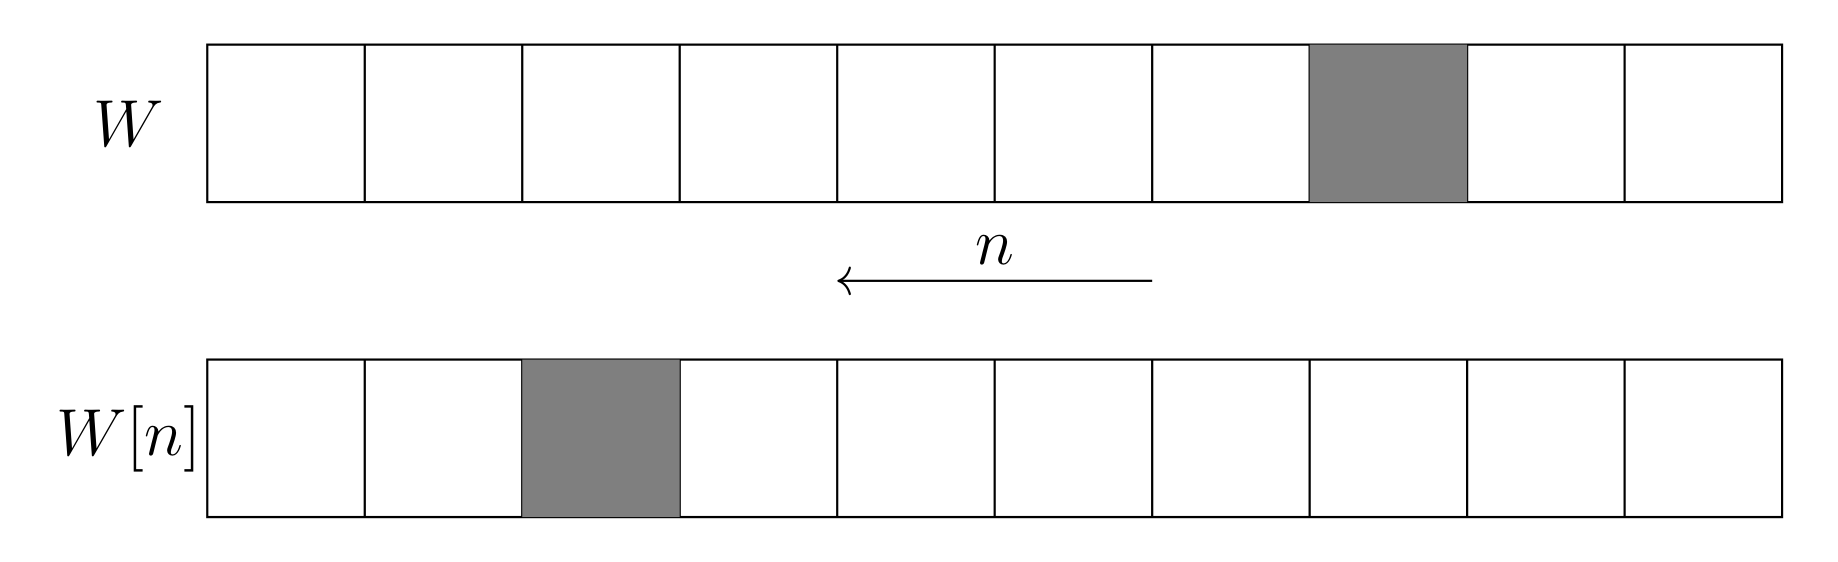
\includegraphics[width=0.74\linewidth]{fig_p025_1.png}
  \caption*{次数平移 $W\to W[n]$ 的示意图（原文 PDF p.25 示意图，原文无编号）}
\end{figure}

  \item $W^{\vee}$ 表示线性对偶，其中
        \[
          (W^{\vee})_m:=\Hom(W_{-m},k)=(W_{-m})^{\vee}.
        \]
  \item 给定两个 $\Z$-分次向量空间 $V,W$：
        \[
          (V\otimes W)_n:=\bigoplus_{i+j=n}(V_i\otimes W_j),
          \qquad
          \Hom(V,W)_n:=\bigoplus_{i}\Hom(V_i,W_{i+n}).
        \]
  \item $\Sym^{m}(V):=V^{\otimes m}/\sim$，其中
        \[
          a\otimes b\sim(-1)^{|a||b|}\,b\otimes a.
        \]
        这称为 $m$ 次\textbf{分次对称张量}。我们记
        \[
          \Sym(V):=\bigoplus_{m\ge0}\Sym^{m}(V),
          \qquad
          \widehat{\Sym}(V):=\prod_{m\ge0}\Sym^{m}(V).
        \]
  \item $\bigwedge^{m}(V):=V^{\otimes m}/\sim$，其中
        \[
          a\otimes b\sim-(-1)^{|a||b|}\,b\otimes a.
        \]
        这称为 $m$ 次\textbf{分次反对称张量}。
\end{itemize}

% [Tutor Note: 记号提醒：$W[n]_m:=W_{n+m}$ 意味着 $W[n]$ 中次数为 $m$ 的元素，原来次数为
% $m+n$，即 shift 把次数整体**降低** $n$。不同文献对 $[n]$ 的约定可能整体差一个符号，
% 引用公式时务必先确认。这里 $[-1]$ 的作用是把“鬼场”次数降 $1$，从而让
% $\mathfrak g^{\vee}[-1]$ 与通常外代数的次数对齐（见命题 4.6）。]

% [Tutor Note: 注意 $\Sym(V)$ 是直和、$\widehat{\Sym}(V)$ 是直积：前者只含有限个非零分量，
% 后者是形式幂级数（可含无穷多项）。原书 p.29 定义 $L_\infty$ 的导子 $\delta$ 时必须用
% 完备化的 $\widehat{\Sym}$，否则无穷和 $\delta=\sum_{n\ge1}\delta_n$ 无意义——
% 这正是原文括号中“so that $\delta$ is defined”的含义。原文 p.25 与 p.29 分别在
% $\Sym$ 上方加宽帽与波浪号，记号不统一，本译本统一写作 $\widehat{\Sym}$。]

\begin{wprop}{4.6}
  $\bigwedge^{k}(V[1])\cong\Sym^{k}(V)[k]$。
\end{wprop}

\begin{proof}
  这是一道很有用也很有益的练习。
\end{proof}

\begin{wdefn}{4.7}
  \textbf{分次 Lie 代数}是一个 $\Z$-分次空间
  \[
    \mathfrak g=\bigoplus_{m\in\Z}\mathfrak g_m,
  \]
  连同双线性映射
  \[
    [-,-]:\ \mathfrak g\otimes\mathfrak g\longrightarrow\mathfrak g,
  \]
  满足以下条件：
  \begin{enumerate}[label=\arabic*),leftmargin=1.8em,itemsep=0.25em]
% >>> p026
    \item 分次括号：$[\mathfrak g_\alpha,\mathfrak g_\beta]
          \subset\mathfrak g_{\alpha+\beta}$；
    \item 分次反对称性：
          \[
            [a,b]=-(-1)^{\alpha\beta}[b,a],
            \qquad\forall a\in\mathfrak g_\alpha,\ b\in\mathfrak g_\beta;
          \]
    \item 分次 Jacobi 恒等式：
          \[
            [[a,b],c]=[a,[b,c]]-(-1)^{\alpha\beta}[b,[a,c]],
            \qquad\forall a\in\mathfrak g_\alpha,\ b\in\mathfrak g_\beta,\
            c\in\mathfrak g_\gamma.
          \]
  \end{enumerate}
\end{wdefn}

% [Tutor Note: 分次 Jacobi 恒等式的符号 $(-1)^{\alpha\beta}$ 来自把次数为 $\alpha$ 的 $a$
% 移过次数为 $\beta$ 的 $b$。三条公理中符号最易记错的是这一条：若漏掉 $(-1)^{\alpha\beta}$
% 或把它写成 $(-1)^{\beta\gamma}$，$\dd_{\mathrm{CE}}^2=0$ 立刻失效。此外要注意原文的配对方式
% 是 $[a,[b,c]]$ 与 $[b,[a,c]]$，一旦改写成别的字母顺序，指数也要相应改变，务必重新推导
% 而不要硬背。]

\begin{wdefn}{4.8}
  \textbf{微分分次 Lie 代数}（DGLA）是一个分次 Lie 代数 $\mathfrak g$，连同
  一个次数为 $1$ 的线性映射 $\dd$（即 $\dd:\mathfrak g_m\to\mathfrak g_{m+1}$），满足
  \begin{enumerate}[label=\arabic*),leftmargin=1.8em,itemsep=0.25em]
    \item $\dd^2=0$，故 $(\mathfrak g,\dd)$ 是一个上链复形；
    \item 分次 Leibniz 法则：
          \[
            \dd[a,b]=[\dd a,b]+(-1)^{\alpha}[a,\dd b],
            \qquad\forall a\in\mathfrak g_\alpha,\ b\in\mathfrak g_\beta.
          \]
  \end{enumerate}
\end{wdefn}

\begin{wexam}{4.9}
  通常的 Lie 代数就是如下的 DGLA：
  \begin{itemize}[leftmargin=1.6em,itemsep=0.2em]
    \item $\mathfrak g=\mathfrak g_0$ 集中在次数 $=0$ 处；
    \item $\dd=0$。
  \end{itemize}
  因此 DGLA 是 Lie 代数的自然推广。
\end{wexam}

\begin{wexam}{4.10}
  设 $X$ 是一个流形，$\mathfrak g$ 是一个 Lie 代数。设 $(\Omega^{\bullet}(x),\dd)$ 是
  de Rham 复形。则 $(\Omega^{\bullet}(x)\otimes\mathfrak g,\,\dd,\,[-,-])$ 是一个 DGLA。
  \begin{itemize}[leftmargin=1.6em,itemsep=0.2em]
    \item $\Omega^{p}(x)\otimes\mathfrak g$ 是次数为 $p$ 的分量。
    \item $\dd:\Omega^{p}(x)\otimes\mathfrak g\to\Omega^{p+1}(x)\otimes\mathfrak g$ 是
          de Rham 微分：
          \[
            \dd(\alpha\otimes h)=\dd\alpha\otimes h,
            \qquad\text{对 } \alpha\in\Omega^{p},\ h\in\mathfrak g.
          \]
    \item 括号由 $\mathfrak g$ 上的 Lie 括号 $[-,-]_{\mathfrak g}$ 诱导：
          \[
            [\alpha_1\otimes h_1,\alpha_2\otimes h_2]
            :=(\alpha_1\wedge\alpha_2)\otimes[h_1,h_2]_{\mathfrak g},
            \qquad\forall\alpha_1,\alpha_2\in\Omega^{*},\ h_1,h_2\in\mathfrak g.
          \]
  \end{itemize}
  这个例子与 Chern--Simons 理论相关。
\end{wexam}

\begin{wexam}{4.11}
  设 $X$ 是一个复流形。设 $(\Omega^{0,\bullet},\bar\partial)$ 是 Dolbeault 复形。
  用 $T^{1,0}_X$ 表示 $(1,0)$-向量场丛。则
  \[
    \bigl(\Omega^{0,\bullet}\bigl(X,T^{1,0}_X\bigr),\,
    \bar\partial,\,[-,-]\bigr)
  \]
  是一个 DGLA。具体地，设 $z^i$ 是局部全纯坐标。元素
  $\alpha\in\Omega^{0,p}\bigl(X,T^{1,0}_X\bigr)$ 可写成
  \[
    \alpha=\sum_{i,J}\alpha^{i}_{J}\,\dd\bar z^{J}\otimes
    \frac{\partial}{\partial z^{i}}.
  \]
  这里 $J=\{j_1<\cdots<j_p\}$ 是一个多重指标，且
  $\dd\bar z^{J}=\dd\bar z^{j_1}\wedge\cdots\wedge \dd\bar z^{j_p}$。于是微分为
  \[
    \bar\partial\alpha
    =\sum\bar\partial\bigl(\alpha^{i}_{J}\bigr)\wedge \dd\bar z^{J}\otimes
    \frac{\partial}{\partial z^{i}}
    =\sum_{l}\frac{\partial\alpha^{i}_{J}}{\partial\bar z^{l}}\,
    \dd\bar z^{l}\wedge \dd\bar z^{J}\otimes\frac{\partial}{\partial z^{i}}.
  \]
\end{wexam}

% >>> p027
给定两个元素
\[
  \alpha=\sum\alpha^{i}_{J}\,\dd\bar z^{J}\otimes\frac{\partial}{\partial z^{i}},
  \qquad
  \beta=\sum\beta^{i}_{M}\,\dd\bar z^{M}\,\frac{\partial}{\partial z^{i}},
\]
它们的括号由下式给出：
\[
  [\alpha,\beta]
  =\sum\Bigl(\alpha^{i}_{J}\frac{\partial\beta^{i}_{M}}{\partial z^{j}}
  -\beta^{i}_{M}\frac{\partial\alpha^{i}_{J}}{\partial z^{j}}\Bigr)
  \dd\bar z^{J}\wedge \dd\bar z^{M}\otimes\frac{\partial}{\partial z^{i}}.
\]
在次数 $=0$ 的分量上，这恰好是 $(1,0)$-向量场上通常的 Lie 括号。

% [Tutor Note: 原文疑误（指标错位）：括号公式中 $\alpha$ 与 $\beta$ 的上指标都印成了 $i$，
% 而求导变量是 $z^{j}$。按定义应为
% $\alpha^{j}_{J}\partial_j\beta^{i}_{M}-\beta^{j}_{M}\partial_j\alpha^{i}_{J}$
% （上指标 $j$ 与求导变量缩并、$i$ 是向量场指标，$\sum_{i,J,M}$ 之外还隐含对 $j$ 求和）。
% 此外 $\beta$ 的展开式原文漏印了 $\otimes$（印成
% $\beta^{i}_{M}\dd\bar z^{M}\frac{\partial}{\partial z^{i}}$），宜读作
% $\beta^{i}_{M}\dd\bar z^{M}\otimes\frac{\partial}{\partial z^{i}}$。均照录原文，请核对
% 原书 p.26--27 / PDF p.26--27。同类排印不一致还见于例 4.10：流形先记 $X$，其后公式里
% 却一律写作小写 $x$（$\Omega^{\bullet}(x)$），本译本照录原文，读者应读作 $X$。]

这个 DGLA 与复结构的形变有关。在物理上，它与 B-扭曲拓扑弦场论
（Kodaira--Spencer 引力）相关。

Chevalley--Eilenberg 复形的构造可以自然地推广到 DGLA。设
$(\mathfrak g,\dd,[-,-])$ 是一个 DGLA。定义分次空间
\[
  C^{\bullet}(\mathfrak g):=\Sym\bigl(\mathfrak g^{\vee}[-1]\bigr)
  =\bigoplus_{m}\Sym^{m}\bigl(\mathfrak g^{\vee}[-1]\bigr).
\]
由于 $\mathfrak g^{\vee}[-1]=(\mathfrak g[1])^{\vee}$，我们可以把
$C^{\bullet}(\mathfrak g)$ 看作 $\mathfrak g[1]$ 上的（多项式）函数。当 $\mathfrak g$
是通常的 Lie 代数时，命题 4.6 蕴含
\[
  C^{k}(\mathfrak g)=\Sym^{k}\bigl(\mathfrak g^{\vee}[-1]\bigr)
  \simeq\bigwedge{}^{k}\mathfrak g^{\vee}[-k],
\]
即 $\bigwedge^{k}\mathfrak g^{\vee}$ 位于次数 $k$ 处。令
\begin{itemize}[leftmargin=1.6em,itemsep=0.3em]
  \item $\dd:\mathfrak g\to\mathfrak g$ 的对偶为
        \[
          \dd_1:\ \mathfrak g^{\vee}[-1]\longrightarrow\mathfrak g^{\vee}[-1];
        \]
  \item 括号 $[-,-]:\bigwedge^{2}\mathfrak g\to\mathfrak g$ 的对偶为
        \[
          \dd_2:\ \mathfrak g^{\vee}[-1]\longrightarrow
          \Sym^{2}\bigl(\mathfrak g^{\vee}[-1]\bigr)
          \simeq\bigwedge{}^{2}\mathfrak g^{\vee}[-2].
        \]
\end{itemize}
注意 $\dd_1$ 与 $\dd_2$ 的次数均为 $1$。由于 $C^{\bullet}(\mathfrak g)$ 由
$\mathfrak g^{\vee}[-1]$ 自由生成，我们可以按以下方式把 $\dd_1$ 与 $\dd_2$ 延拓到
$C^{\bullet}(\mathfrak g)$ 上：
\begin{itemize}[leftmargin=1.6em,itemsep=0.3em]
  \item 在生成元 $\mathfrak g^{\vee}[-1]$ 上，按上述定义；
  \item 分次 Leibniz 法则：对 $\dd=\dd_1$ 或 $\dd_2$，
        \[
          \dd(a\wedge b)=(\dd a)\wedge b+(-1)^{|a|}\,a\wedge \dd b.
        \]
\end{itemize}
定义 \textbf{Chevalley--Eilenberg 微分}
\[
  \dd_{\mathrm{CE}}=\dd_1+\dd_2:\ C^{\bullet}(\mathfrak g)\longrightarrow
  C^{\bullet}(\mathfrak g).
\]

% [Tutor Note: 为什么对 DGLA 的 CE 复形要用 $\Sym(\mathfrak g^{\vee}[-1])$ 而不是
% $\bigwedge^{\bullet}\mathfrak g^{\vee}$？对集中在 $0$ 次的通常 Lie 代数，两者由命题 4.6
% 同构（$k$ 次部分都落在次数 $k$）；但对一般 DGLA，$\mathfrak g$ 自身带奇偶，
% 只有 $\Sym$ 才是“$\mathfrak g[1]$ 上的函数环”，$\bigwedge^{\bullet}$ 会给出错误的符号。
% 这一点在第 6 章 BV 形式中至关重要：那里 $C^{\bullet}(\mathfrak g)$ 就是多向量场代数。
% 另注：上式 $\dd(a\wedge b)$ 中的“$\wedge$”是原文写法，在对称代数里其实是乘法
% （可写成 $\dd(ab)$），原文记号混用；照着读即可。]

\begin{wprop}{4.12}
  $\dd_{\mathrm{CE}}^2=0$。复形 $(C^{\bullet}(\mathfrak g),\dd_{\mathrm{CE}})$ 也称为
  Chevalley--Eilenberg 上链复形。
\end{wprop}

\begin{proof}[证明梗概]
  我们说明为何这是对的，细节留给读者。事实上，如果我们把
  $\dd_{\mathrm{CE}}$ 表示为
\begin{figure}[htbp]
  \centering
  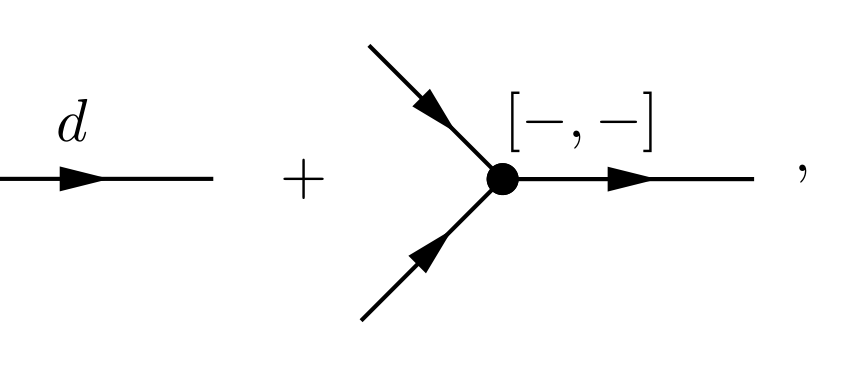
\includegraphics[width=0.35\linewidth]{fig_p027_1.png}
  \caption*{$\dd_{\mathrm{CE}}$ 的图形表示（原文 PDF p.27 示意图，原文无编号）}
\end{figure}
% >>> p028
  那么我们有
\begin{figure}[htbp]
  \centering
  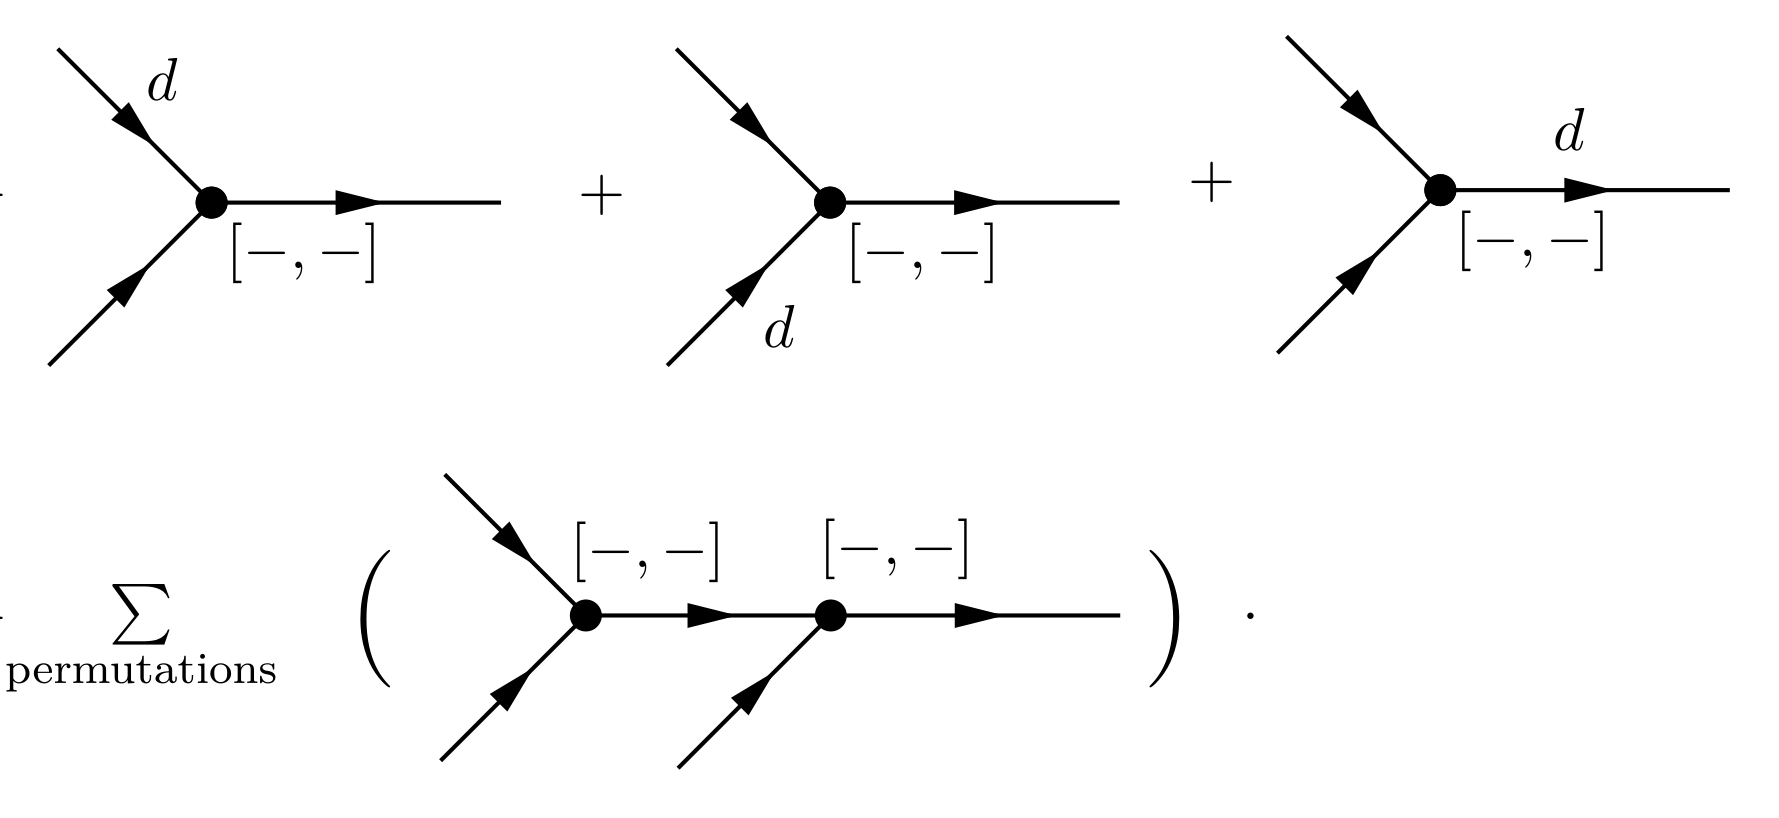
\includegraphics[width=0.71\linewidth]{fig_p028_1.png}
  \caption*{$\dd_{\mathrm{CE}}^2=0$ 的图形展开（原文 PDF p.28 示意图，原文无编号）}
\end{figure}
  我们可以“看出”，$\dd_{\mathrm{CE}}^2=0$ 等价于 DGLA 的定义性质：
  \begin{itemize}[leftmargin=1.6em,itemsep=0.2em]
    \item $\dd^2=0$，
    \item Leibniz 法则：$\dd[-,-]=[\dd(-),-]\pm[-,\dd(-)]$，
    \item Jacobi 恒等式。
  \end{itemize}
\end{proof}

% [Tutor Note: 图形证明里的“$\sum$ permutations”一项不能漏：$\dd_{\mathrm{CE}}^2$ 的四类图
% 分别对应 DGLA 的三条公理——直线 $\dd^2=0$；$\dd$ 与顶点的两种相对位置给出分次 Leibniz
% 法则（差一个 Koszul 符号）；两个顶点复合的置换和给出 Jacobi 恒等式。把图翻译成公式时，
% 每个三价顶点贡献一个括号、每条标 $\dd$ 的线贡献一次 $\dd$，而“外线的排列”贡献符号。
% 这套“图$\,=\,$公式”的翻译规则在第 5 章的 Feynman 图展开中会系统化。]

推广到 $\mathfrak g$-模是直接的。

\begin{wdefn}{4.13}
  设 $\mathfrak g$ 是一个 DGLA。一个 \textbf{$\mathfrak g$-模}是一个上链复形
  $(M,\dd_M)$，连同双线性映射 $\mathfrak g\otimes M\xrightarrow{\ \cdot\ }M$，满足
  \begin{itemize}[leftmargin=1.6em,itemsep=0.25em]
    \item $\mathfrak g_\alpha\otimes M_\beta\longrightarrow M_{\alpha+\beta}$；
    \item $a\cdot(b\cdot m)-(-1)^{\alpha\beta}\,b\cdot(a\cdot m)=[a,b]\cdot m$，
          $\forall a\in\mathfrak g_\alpha,\ b\in\mathfrak g_\beta,\ m\in M$；
    \item $\dd_M(a\cdot m)=(\dd a)\cdot m+(-1)^{\alpha}\,a\cdot \dd_M m$，
          $\forall a\in\mathfrak g_\alpha,\ m\in M$。
  \end{itemize}
\end{wdefn}

等价地，让我们定义分次空间
\[
  \mathfrak g_M:=\mathfrak g\oplus M,
\]
并赋予微分 $\dd\oplus \dd_M$ 与括号 $[-,-]$，其中
\begin{itemize}[leftmargin=1.6em,itemsep=0.2em]
  \item 在 $\mathfrak g\otimes\mathfrak g$ 上，$[-,-]$ 是 $\mathfrak g$ 上的括号：
        $[-,-]:\mathfrak g\otimes\mathfrak g\to\mathfrak g$；
  \item 在 $\mathfrak g\otimes M$ 上，$[-,-]$ 是 $\mathfrak g$-模作用：
        $[-,-]:\mathfrak g\otimes M\to M$；
  \item 在 $M\otimes M$ 上，$[-,-]=0$。
\end{itemize}
于是
\[
  M\ \text{是}\ \mathfrak g\text{-模}\iff\mathfrak g_M\ \text{是 DGLA}.
\]
相应的 Chevalley--Eilenberg 复形是
\[
  C^{\bullet}(\mathfrak g,M)
  :=\bigl(\Sym(\mathfrak g^{\vee}[-1])\otimes M,\,\dd_{\mathrm{CE}}\bigr).
\]
$\dd_{\mathrm{CE}}$ 的描述我们留给读者。

% [Tutor Note: 第二组条件（$M\otimes M$ 上的括号取 $0$）说明 $\mathfrak g_M$ 是“半直积”
% Lie 代数 $\mathfrak g\ltimes M$ 的分次版本；而 $M\otimes M$ 上的括号为零，正是
% “$M$ 是模”而非“$M$ 是子代数”的代数表述。第一条式子
% $a\cdot(b\cdot m)-(-1)^{\alpha\beta}b\cdot(a\cdot m)=[a,b]\cdot m$ 就是分次 Jacobi
% 恒等式在 $\mathfrak g\oplus M$ 上的投影，写成分次形式时那个 $(-1)^{\alpha\beta}$ 极易漏掉。]

% >>> p029
\subsection{同伦 Lie 代数（Homotopy Lie Algebra，$L_\infty$-代数）}

给定一个分次向量空间 $V$，考虑 $\Sym(V)$ 上次数为 $1$ 的导子（derivation）
\[
  \delta:\ \Sym(V)\longrightarrow\Sym(V),
\]
它满足分次 Leibniz 法则
\[
  \delta(a\otimes b)=(\delta a)\otimes b+(-1)^{|a|}\,a\otimes\delta b.
\]
这样的 $\delta$ 完全由它在生成元上的作用决定：
\[
  \delta:\ V\longrightarrow\Sym(V).
\]
我们可以分解
\[
  \delta=\delta_0+\delta_1+\delta_2+\cdots,
\]
其中 $\delta_k:V\to\Sym^{k}(V)$。对 DGLA，我们有
\[
  \delta=\dd_{\mathrm{CE}}=\dd_1+\dd_2=\delta_1+\delta_2.
\]
这是一个只有 $\delta_1,\delta_2$ 非平凡的导子。把所有可能的分量 $\delta_k$ 都编码进来，
自然地推广这一算子，就引出了 $L_\infty$-代数。

% [Tutor Note: 原文从 $\delta_0$ 开始分解，但紧接着又只要求 $\delta_k:V\to\Sym^{k}(V)$，
% 而 $\Sym^{0}(V)=k$，故 $\delta_0$ 是一个次数 $1$ 的线性泛函 $V\to k$（仅当 $V$ 有
% $-1$ 次分量时可能非零）。通常的 $L_\infty$ 展开从 $\delta_1$ 起；$\delta_0\ne0$ 的情形
% 称为“弯曲”的（curved）$L_\infty$ 代数，本课程用不到。对 DGLA 有 $\delta_0=0$，
% 故原文随即写出 $\delta=\dd_1+\dd_2=\delta_1+\delta_2$。]

\begin{wdefn}{4.14}
  一个 \textbf{$L_\infty$-代数}是一个 $\Z$-分次向量空间 $\mathfrak g$，连同一族多重线性映射
  \[
    \ell_n:\ \bigwedge{}^{n}\mathfrak g\longrightarrow\mathfrak g,
    \qquad \deg(\ell_n)=2-n\quad(n\ge1),
  \]
  满足以下的 \textbf{$L_\infty$-关系式}
  \[
    \sum_{k=1}^{n}\pm\,\ell_{n-k+1}\bigl(\ell_k(\cdots),\cdots\bigr)=0,
    \qquad\forall n.
  \]
\end{wdefn}

% [Tutor Note: $\deg(\ell_n)=2-n$ 的正确性可用两个低阶项校验：$\ell_1$ 的次数为
% $2-1=1$，即微分（$\dd$）；$\ell_2$ 的次数为 $2-2=0$，即通常的 Lie 括号；$\ell_3,\ell_4,\dots$
% 是“高阶括号”，它们使得 Jacobi 恒等式只在同伦意义下成立。若把次数记成 $1-n$ 或
% $n-2$，则对偶侧导子 $\delta_n$ 的次数就不再是 $1$，整个构造失效。]

这种复杂的 $L_\infty$-关系可以这样理解。令
\[
  \delta_n:\ \mathfrak g^{\vee}[-1]\longrightarrow
  \Sym^{n}\bigl(\mathfrak g^{\vee}[-1]\bigr)
  \simeq\bigwedge{}^{n}\mathfrak g^{\vee}[-n]
\]
表示 $\ell_n:\bigwedge^{n}\mathfrak g\to\mathfrak g$ 的对偶。注意
\[
  \deg(\ell_n)=2-n\iff\deg(\delta_n)=1.
\]
令 $\delta=\sum_{n\ge1}\delta_n=\delta_1+\delta_2+\cdots$，它通过分次 Leibniz 法则定义了
$C^{\bullet}(\mathfrak g)=\widehat{\Sym}\bigl(\mathfrak g^{\vee}[-1]\bigr)$ 上的一个导子。
（这里我们使用（分次的）形式幂级数环
$\widehat{\Sym}\bigl(\mathfrak g^{\vee}[-1]\bigr)$，以保证 $\delta$ 有定义。）于是
\[
  \{\ell_n\}_{n\ge1}\ \text{的 } L_\infty\text{-关系}
  \iff \delta^2=0 .
\]
$(C^{\bullet}(\mathfrak g),\delta)$ 是 $\mathfrak g$ 的 Chevalley--Eilenberg 复形。

如果对每个 $\delta_n$ 都画一张图
\begin{figure}[htbp]
  \centering
  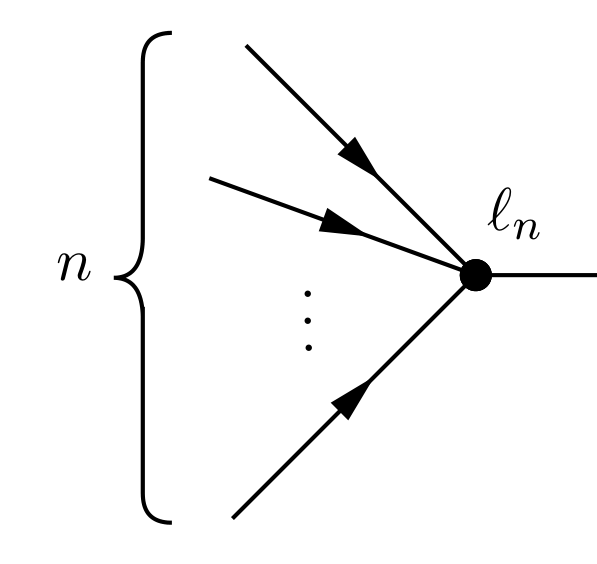
\includegraphics[width=0.24\linewidth]{fig_p029_1.png}
  \caption*{$\delta_n$ 的图形表示（原文 PDF p.29 示意图，原文无编号）}
\end{figure}
% >>> p030
那么 $\delta^2=0$ 可以画成
\begin{figure}[htbp]
  \centering
  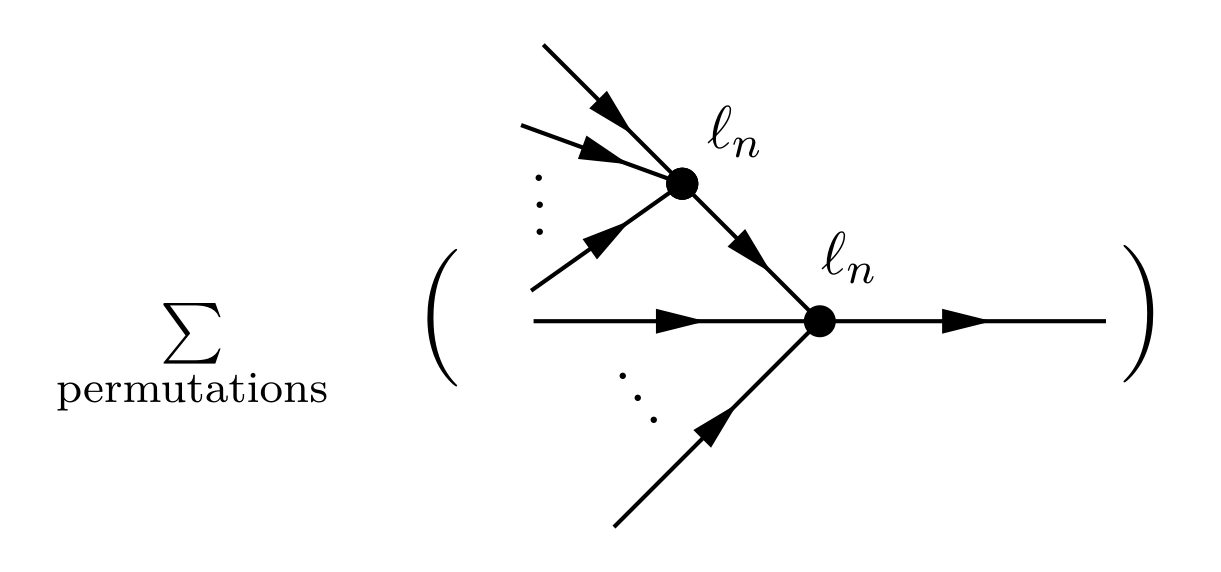
\includegraphics[width=0.49\linewidth]{fig_p030_1.png}
  \caption*{$\delta^2=0$ 的图形表示（原文 PDF p.30 示意图，原文无编号）}
\end{figure}
正如我们将看到的，这通过 Feynman 图技术有一个自然的解释。关于 $L_\infty$-代数及其与
QFT 的关系，一个很好的综述见文献 [27] 及其参考文献。

% [Tutor Note: $L_\infty$-关系式里的“$\pm$”不是可有可无的装饰：它是 Koszul 符号，
% 由把次数为 $2-k$ 的映射 $\ell_k$ 移过其余输入所产生。$n=2$ 时该式化为
% $\ell_1\ell_2=\ell_2(\ell_1\otimes1\pm1\otimes\ell_1)$，即“$\ell_1$ 是 $\ell_2$ 的导子”
% （分次 Leibniz 法则）；$n=3$ 时它给出 Jacobi 恒等式的同伦修正：
% $\ell_1\ell_3+\ell_3\ell_1$ 与 $\ell_2\ell_2$ 只差一个 Koszul 符号的轮换和。
% 直接照抄别人的符号表是危险的——务必按“映射次数 + 输入置换”自行重算。]

% [Tutor Note: 物理图像点拨：$\delta^2=0$ 的图恒等式正是量子场论中 Ward 恒等式/
% 主方程的雏形——一个 $\ell_n$ 顶点代表 $n$ 个场的一次相互作用，$\delta^2=0$ 说
% “把所有可能的收缩方式加起来为零”。第 5 章的 Wick 定理与 Feynman 图展开、第 6--7 章的
% BV 主方程都会以不同的语言重复这张图。原文引用的 [27] 见书末参考文献。]


% ---------- part05.tex ----------
% ============================================================
%  part05.tex  |  原文 PDF p.31–40（页脚 p.30–39）
%  内容：第 5 章 微扰展开（Perturbative Expansion）
%        5.1 Wick 定理（PDF p.31–34）
%        5.2 Feynman 图展开（PDF p.34–38）
%        5.3 Green 函数（PDF p.38–39）
%        5.4 正则量子化（PDF p.40；仅标题与开头两段，续文见 part06）
% ============================================================

% >>> p031
\section{微扰展开（Perturbative Expansion）}

\begin{keypoints}
  \item \textbf{核心物理图像}：微扰论把路径积分按耦合常数 $\lambda$ 展开，每一项对应一张
        Feynman 图——图是“相互作用如何把场配成对”的组合记账本，而数值由 Wick 定理
        逐边赋权得到。
  \item \textbf{数学工具}：有限维 Gaussian 积分与期望 $\langle-\rangle_x$、Wick 定理
        （对 $P(2m)$ 的配对求和）、图的公理化定义（顶点/半边/边/入射映射）、
        自同构群 $\Aut(\Gamma)$、Euler 示性数与圈数 $l(\Gamma)$。
  \item \textbf{主要结论}：Wick 定理给出
        $\bigl\langle x^{i_1}\cdots x^{i_{2m}}\bigr\rangle_x
        =\hbar^m\sum_{\sigma\in P(2m)}\prod_{k=1}^{m}
        (Q^{-1})^{\sigma(2k-1)\sigma(2k)}$；图的求和公式中每张图带权
        $\hbar^{l(\Gamma)-1}\omega_\Gamma/|\Aut(\Gamma)|$，且连通图部分取指数。
  \item \textbf{译者评注}：本节是后面所有计算的“发动机”：$1/|\Aut(\Gamma)|$ 因子
        （自同构/对称因子）与 $\hbar$ 的幂次是最常出错的两处。5.3 节把同一套组合规则
        搬到无穷维场论，得到用 Green 函数（传播子）表达的关联函数；5.4 节则转入
        正则量子化，为 part06 的 UV 发散与重整化作准备。
\end{keypoints}

在量子场论中，我们关心可观测量 $\mathcal O$ 的量子关联，它是一个无穷维积分
\[
  \int_{\mathcal E}\ee^{\frac{\ii S}{\hbar}}\mathcal O[D\phi].
\]
这种测度的严格构造在一般情况下尚不清楚。尽管如此，关于 $\hbar\to0$ 的渐近理论
已经作为微扰重整化方法建立起来。

\subsection{Wick 定理（Wick's Theorem）}

\paragraph{高斯积分（Gaussian Integral）}
我们从有限维情形开始。设
\[
  Q(x)=\sum_{i,j=1}^{n}Q_{ij}x^{i}x^{j}
\]
是一个正定二次型，即矩阵 $(Q_{ij})$ 正定。考虑 $\R^n$ 上的如下体积形式
\[
  \Omega=\sqrt{\det Q}\prod_{i=1}^{n}\frac{\dd x^{i}}{\sqrt{2\pi\hbar}}\,
  \ee^{-\frac{1}{2\hbar}Q(x)},
  \qquad \hbar>0.
\]
由高斯积分 $\int_{\R}\dd x\,\ee^{-\frac{1}{2}x^{2}}=\sqrt{2\pi}$ 容易看出
\[
  \int_{\R^{n}}\Omega=1.
\]
于是 $\Omega$ 定义了 $\R^n$ 上的一个概率密度。

为简单起见，考虑多项式函数 $f(x)\in\R[x^{i}]$。定义关于概率密度 $\Omega$ 的如下期望值：
\[
  \langle f(x)\rangle_x
  :=\frac{\int_{\R^{n}}\Omega\,f(x)}{\int_{\R^{n}}\Omega}
  =\int_{\R^{n}}\Omega\,f(x).
\]
下标 $x$ 表示积分变量。这个期望值定义了映射
\[
  \langle-\rangle_x:\ \R[x^{i}]\longrightarrow\R.
\]
为计算这一期望映射，我们考虑辅助积分
\[
  \begin{aligned}
    Z[J]&:=\left\langle \ee^{\sum_{i}x^{i}J_i}\right\rangle_x,
    \qquad J=(J_1,\cdots,J_n)\\
    &=\sqrt{\det Q}\int_{\R^{n}}\prod_{i=1}^{n}\frac{\dd x^{i}}{\sqrt{2\pi\hbar}}\,
    \ee^{-\frac{1}{2\hbar}Q(x)+\sum_{i}x^{i}J_i}.
  \end{aligned}
\]
配方可得
\[
  \frac{1}{2\hbar}Q(x)-\sum_{i}x^{i}J_i
  =\frac{1}{2\hbar}Q\Bigl(x^{i}-\hbar\sum_{j}(Q^{-1})^{ij}J_j\Bigr)
  -\frac{\hbar}{2}Q^{-1}(J).
\]

% [Tutor Note: 高斯积分的常数因子务必逐项核对。做代换
% $x^{i}=\sqrt{\hbar}\sum_{j}(Q^{-1/2})^{i}{}_{j}y^{j}$（矩阵写法
% $x=\sqrt{\hbar}\,Q^{-1/2}y$）时，测度的 Jacobi 因子为
% $\hbar^{n/2}\det(Q)^{-1/2}$。它与 $\Omega$ 中的 $\sqrt{\det Q}$ 以及每维的
% $1/\sqrt{2\pi\hbar}$ 恰好凑成 $\prod_i\dd y^{i}/\sqrt{2\pi}$，同时
% $\frac{1}{2\hbar}Q(x)=\frac{1}{2}|y|^{2}$，于是 $\int\Omega=1$。
% 若把 $\sqrt{\det Q}$ 写成 $\det Q$，或忘记测度里 $\hbar^{n/2}$ 的幂次，
% $\int\Omega=1$ 立刻不成立，后续所有期望值也会整体差 $\hbar$ 的幂。
% 习题：在 $n=1$、$Q=q$ 时逐项验证。]

% >>> p032
这里 $(Q^{-1})^{ij}$ 是 $Q_{ij}$ 的逆矩阵
\[
  \sum_{k}Q_{ik}(Q^{-1})^{kj}=\delta_i^{\ j},
\]
而 $Q^{-1}(J)$ 是二次表达式
\[
  Q^{-1}(J)=\sum_{i,j}(Q^{-1})^{ij}J_iJ_j.
\]
于是
\[
  Z[J]=\ee^{\frac{\hbar}{2}Q^{-1}(J)}\int_{\R^{n}}\Omega
  =\ee^{\frac{\hbar}{2}Q^{-1}(J)}.
\]
现在对多项式 $f(x)$，在 $x=0$ 处的 Taylor 级数展开给出
\[
  f(x)=\ee^{\sum_{i}x^{i}\frac{\partial}{\partial a^{i}}}f(a)\Big|_{a=0}.
\]
利用这个公式，我们得到
\[
  \begin{aligned}
    \langle f(x)\rangle_x
    &=\left\langle
    \ee^{\sum_{i}x^{i}\frac{\partial}{\partial a^{i}}}f(a)\Big|_{a=0}
    \right\rangle_x\\
    &\overset{J=\frac{\partial}{\partial a}}{=}
    Z\left[\frac{\partial}{\partial a}\right]f(a)\Big|_{a=0}
    =\ee^{\frac{\hbar}{2}Q^{-1}\left(\frac{\partial}{\partial a}\right)}
    f(a)\Big|_{a=0},
  \end{aligned}
\]
其中
\[
  Q^{-1}\Bigl(\frac{\partial}{\partial a}\Bigr)
  =\sum_{i,j}(Q^{-1})^{ij}\frac{\partial}{\partial a^{i}}
  \frac{\partial}{\partial a^{j}}
\]
是一个二阶微分算子。

% [Tutor Note: 配方的符号只需用一维情形检验：$\frac{1}{2\hbar}qx^{2}-xJ
% =\frac{1}{2\hbar}q\bigl(x-\hbar J/q\bigr)^{2}-\frac{\hbar}{2}J^{2}/q$，
% 故 $Z[J]=e^{\frac{\hbar}{2}Q^{-1}(J)}$ 的指数是**正**的，且分母里的 $\hbar$
% 使指数无量纲。若把符号弄反（写成 $e^{-\frac{\hbar}{2}Q^{-1}}$），
% 后续 Wick 收缩会整体多一个 $(-1)^m$。多分量时还要注意 $Q^{-1}(J)$ 中
% $J_iJ_j$ 的对称性使 $1/2$ 自动被吸收，不要重复除以 $2$。]

\paragraph{Wick 定理（Wick's Theorem）}
所得的公式
\[
  \langle f(x)\rangle_x
  =\ee^{\frac{\hbar}{2}Q^{-1}\left(\frac{\partial}{\partial a}\right)}
  f(a)\Big|_{a=0}
\]
有如下组合解释。设
\[
  i_1,i_2,\cdots,i_{2m}\in\{1,2,\cdots,n\}
\]
是 $2m$ 个指标。我们考虑由该指标集得到的 $2m$ 次单项式
$x^{i_1}x^{i_2}\cdots x^{i_{2m}}$。由上述公式计算它的期望：
\begin{equation*}
  \begin{aligned}
    \bigl\langle x^{i_1}x^{i_2}\cdots x^{i_{2m}}\bigr\rangle_x
    &=\ee^{\frac{\hbar}{2}Q^{-1}\left(\frac{\partial}{\partial a}\right)}
    a^{i_1}a^{i_2}\cdots a^{i_{2m}}\Big|_{a=0}\\
    &=\frac{\hbar^{m}}{m!}\left[\frac{1}{2}\sum_{i,j}(Q^{-1})^{ij}
    \frac{\partial}{\partial a^{i}}\frac{\partial}{\partial a^{j}}\right]^{m}
    a^{i_1}a^{i_2}\cdots a^{i_{2m}}.
  \end{aligned}
  \tag*{$*$}
\end{equation*}

% [Tutor Note: 上式右端的 $(*)$ 是原文自带的公式标号（全书仅此一处用 $(*)$）；
% 本译本按体例用 \texttt{\textbackslash tag*\{\$*\$\}} 保留在 equation* 中。
% 中间的等号只是把 $e^{\frac{\hbar}{2}Q^{-1}(\partial_a)}$ 按 Taylor 级数展开：
% $e^{\frac{\hbar}{2}Q^{-1}(\partial_a)}=\sum_{m}\frac{1}{m!}
% \bigl(\frac{\hbar}{2}Q^{-1}(\partial_a)\bigr)^{m}$，把每个 $\hbar/2$ 拆成
% $\hbar\cdot\frac{1}{2}$ 就得到 $\hbar^{m}/m!\,[\frac{1}{2}\sum\cdots]^{m}$。
% 这里的 $1/m!$ 与括号内的 $1/2$ 各有来源，不可互相吞并。]

为计算这个值，令
\[
  P(2m)=\Bigl\{\{1,2,\cdots,2m\}\text{ 分成 }m\text{ 个无序对的划分}\Bigr\}.
\]
$P(2m)$ 中的元素 $\sigma$ 可由一个置换 $\sigma\in S_{2m}$ 描述，使得
\[
  \sigma(1)<\sigma(2),\quad \sigma(3)<\sigma(4),\quad\cdots,\quad
  \sigma(2m-1)<\sigma(2m),
\]
并且
\[
  \sigma(1)<\sigma(3)<\cdots<\sigma(2m-3)<\sigma(2m-1).
\]

% >>> p033
然后我们把这一置换
\[
  \begin{bmatrix}
    1 & 2 & 3 & \cdots & 2m-1 & 2m\\
    \sigma(1) & \sigma(2) & \sigma(3) & \cdots & \sigma(2m-1) & \sigma(2m)
  \end{bmatrix}
\]
通过配对
\[
  \underbrace{\sigma(1)\sigma(2)}_{\text{pair}}\quad
  \underbrace{\sigma(3)\sigma(4)}_{\text{pair}}\quad\cdots\quad
  \underbrace{\sigma(2m-1)\sigma(2m)}_{\text{pair}}
\]
与 $P(2m)$ 中的一个元素等同起来。在上述公式 $(*)$ 中，经计算它成为如下求和：
\[
  \boxed{
  \bigl\langle x^{i_1}x^{i_2}\cdots x^{i_{2m}}\bigr\rangle_x
  =\hbar^{m}\sum_{\sigma\in P(2m)}
  (Q^{-1})^{\sigma(1)\sigma(2)}(Q^{-1})^{\sigma(3)\sigma(4)}\cdots
  (Q^{-1})^{\sigma(2m-1)\sigma(2m)}
  }.
\]
这称为 \textbf{Wick 定理}。

% [Tutor Note: Wick 定理的求和无重复计数：$P(2m)$ 的参数化要求每一对内部递增
% （$\sigma(1)<\sigma(2)$ 等），且各对的“首项”递增
% （$\sigma(1)<\sigma(3)<\cdots$），这恰好给每个无序配对唯一的代表元。
% 若改成对所有置换求和，就会多出 $2^m m!$ 倍的重复；这正是后面
% $1/(m!(3!)^m)$ 因子的来源。注意 $(Q^{-1})^{\sigma(1)\sigma(2)}$ 的两个指标
% 是 $\sigma$ 的**值**，不是位置。]

我们也可以把每个求和画成图：
\begin{figure}[htbp]
  \centering
  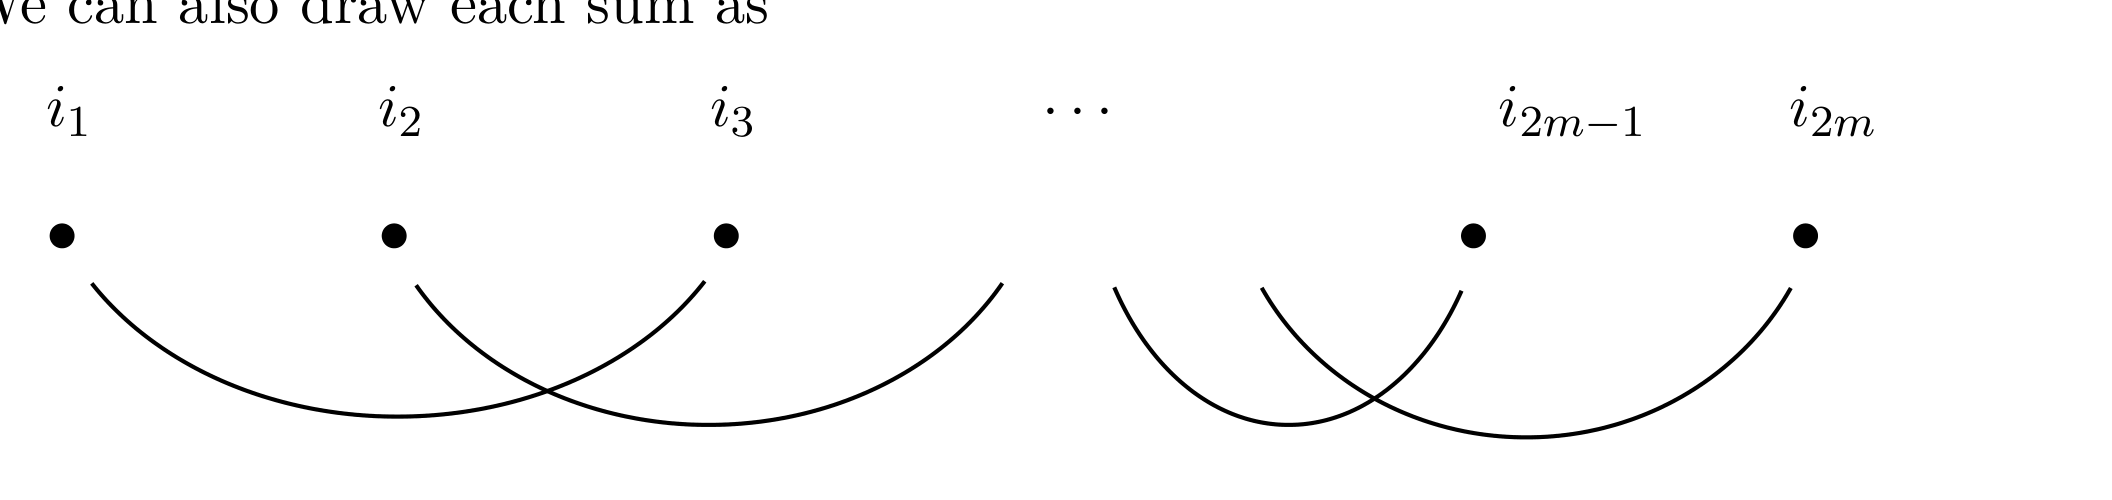
\includegraphics[width=0.85\linewidth]{fig_p033_1.png}
  \caption*{Wick 收缩的配对图（原文 PDF p.33 示意图，原文无编号）}
\end{figure}
对每条连接 $i$ 与 $j$ 的边，我们赋予因子 $\hbar(Q^{-1})^{ij}$。

% [Tutor Note: 图的读数规则是本节的核心：**每个顶点（指标）贡献一个外线，每条边
% （配对）贡献 $\hbar(Q^{-1})^{ij}$**。特别注意因子 $\hbar$——它随边数累积成
% $\hbar^{|E|}$，是后面 $\hbar$ 幂次的唯一来源。漏掉这个 $\hbar$ 会使整张图的
% 量级错一个 $\hbar$ 的幂，而这类错误在小 $m$ 的例子里往往看不出来。]

\begin{wexam}{5.1}（两点函数，Two-point function）
  两点函数
  \[
    \bigl\langle x^{i}x^{j}\bigr\rangle_x=\hbar(Q^{-1})^{ij}
  \]
  由 $Q$ 的逆矩阵给出。$(Q^{-1})^{ij}$ 也称为\textbf{传播子}（propagator）。

\begin{figure}[htbp]
  \centering
  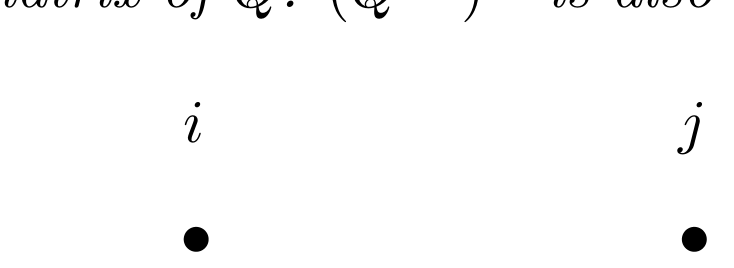
\includegraphics[width=0.29\linewidth]{fig_p033_2.png}
  \caption*{两点函数图（原文 PDF p.33 示意图，原文无编号）}
\end{figure}
\end{wexam}

\begin{wexam}{5.2}
  如下四点函数可由下式计算：
\begin{figure}[htbp]
  \centering
  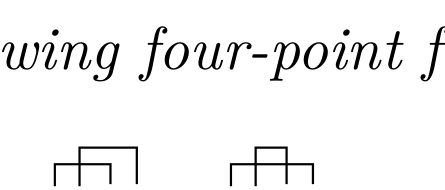
\includegraphics[width=0.22\linewidth]{fig_p033_3.png}
  \caption*{四点函数的三种配对图（原文 PDF p.33 示意图，原文无编号）}
\end{figure}
  \[
    \bigl\langle x^{i}x^{j}x^{k}x^{l}\bigr\rangle_x
    =\hbar^{2}\Bigl[(Q^{-1})^{ij}(Q^{-1})^{kl}
    +(Q^{-1})^{ik}(Q^{-1})^{jl}
    +(Q^{-1})^{il}(Q^{-1})^{jk}\Bigr].
  \]
\end{wexam}

我们还可以通过平移 $x\to x+a$ 来加入“背景”：
\[
  \langle f(x+a)\rangle_x=\int_{\R^{n}}\Omega\,f(x+a),
\]
它现在是 $a$ 的函数。类似的论证给出
\[
  \langle f(x+a)\rangle_x
  =\ee^{\frac{\hbar}{2}Q^{-1}\left(\frac{\partial}{\partial a}\right)}f(a).
\]
若 $f(x)=x^{i_1}x^{i_2}\cdots x^{i_k}$，则此时的 Wick 定理是部分配对（partial pairings）之和：

% >>> p034
\begin{figure}[htbp]
  \centering
  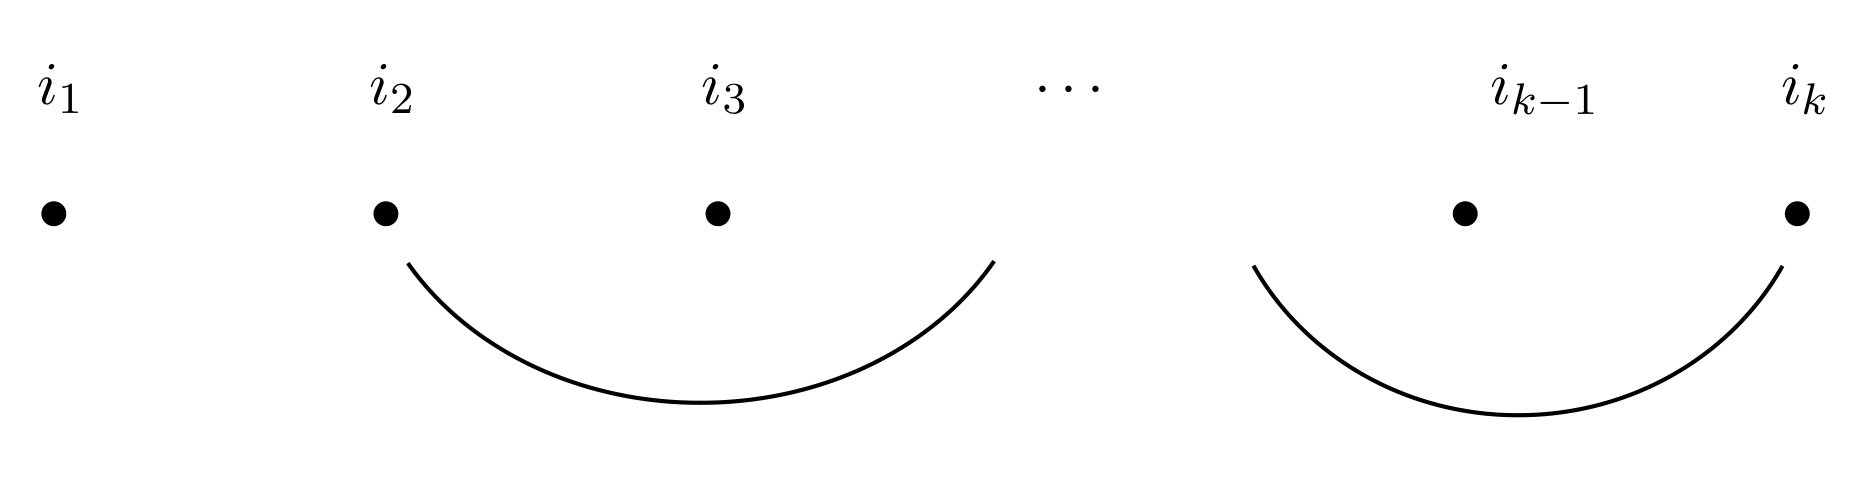
\includegraphics[width=0.75\linewidth]{fig_p034_1.png}
  \caption*{部分配对图（原文 PDF p.34 示意图，原文无编号）}
\end{figure}
我们把传播子赋给已配对的指标，并把 $a^{i}$ 赋给未配对的指标 $i$。

% [Tutor Note: “背景”情形极易算错：$\langle f(x+a)\rangle_x
% =e^{\frac{\hbar}{2}Q^{-1}(\partial_a)}f(a)$ 中，指数算子作用在 $a$ 的函数上，
% 得到的是 $a$ 的**函数**，不是数——不要再取 $a=0$。校验方法：$f$ 为单项式时
% 未配对指标应保留成 $a^{i}$，已配对指标才产生 $\hbar(Q^{-1})$；取 $a=0$ 就退回
% 无背景的 Wick 定理。]

\begin{wexam}{5.3}
  设 $f(x)=x^{i}x^{j}x^{k}x^{l}$。则
  \[
    \begin{aligned}
      \langle f(x+a)\rangle_x
      ={}&a^{i}a^{j}a^{k}a^{l}
      +\hbar\Bigl[(Q^{-1})^{ij}a^{k}a^{l}+(Q^{-1})^{ik}a^{j}a^{l}
      +(Q^{-1})^{il}a^{j}a^{k}\\
      &\qquad\quad+(Q^{-1})^{jk}a^{i}a^{l}+(Q^{-1})^{jl}a^{i}a^{k}
      +(Q^{-1})^{kl}a^{i}a^{j}\Bigr]\\
      &+\hbar^{2}\Bigl[(Q^{-1})^{ij}(Q^{-1})^{kl}
      +(Q^{-1})^{ik}(Q^{-1})^{jl}
      +(Q^{-1})^{il}(Q^{-1})^{jk}\Bigr].
    \end{aligned}
  \]
\end{wexam}

\subsection{Feynman 图展开（Feynman Graph Expansion）}

现在我们考虑如下形式的积分
\[
  \sqrt{\det Q}\int_{\R^{n}}\prod_{i=1}^{n}\frac{\dd x^{i}}{\sqrt{2\pi\hbar}}\,
  \ee^{-\frac{1}{\hbar}S(x)},
\]
其中
\[
  S(x)=\frac{1}{2}Q(x)-\frac{\lambda}{3!}I(x).
\]
这里 $Q(x)=\sum_{i,j}Q_{ij}x^{i}x^{j}$ 是如前所述的正定二次型，而
\[
  I(x)=\sum_{i,j,k}I_{ijk}x^{i}x^{j}x^{k}
\]
是一个三次多项式，称为\textbf{相互作用}（interaction）。常数 $I_{ijk}$ 参数化这些三次型。
常数 $\lambda$ 称为\textbf{耦合常数}（coupling constant）。

由于三次项在 $\pm\infty$ 两端都趋于无穷且增长快于二次项，上述积分干脆就是“发散的”。
要使它有意义，本质上有两条出路：

\begin{itemize}[leftmargin=1.6em,itemsep=0.3em]
  \item ① 把 $x^{i}$ 复化为复变量 $z^{i}$，并把积分围道
        \[
          \R^{n}\subset\C^{n}\qquad\Longrightarrow\qquad \Gamma\subset\C^{n}
        \]
        换到另一条使积分收敛的围道 $\Gamma$ 上。“Airy 积分”就是这样一个例子。
        这种方法通常称为\textbf{非微扰方法}（non-perturbative method）。
  \item ② 把 $\lambda$ 当作微扰参数，计算渐近级数。这种方法通常称为
        \textbf{微扰方法}（perturbative method）。
\end{itemize}

% [Tutor Note: ① 的几何实质是鞍点/最速下降：取使 $\operatorname{Re}S>0$ 的
% Lefschetz 围道即可使积分收敛；原文强调 ② 得到的是**渐近**级数而非收敛级数
% （Dyson 论证：微扰级数一般收敛半径为零），所以 $\hbar\to0$ 的展开只能逐阶使用。
% 把渐近等式当成恒等式，是本节最常见的概念性错误。]

这里我们将聚焦于微扰方法 ②。让我们把
\[
  \text{“}\sqrt{\det Q}\int_{\R^{n}}\prod_{i=1}^{n}\frac{\dd x^{i}}
  {\sqrt{2\pi\hbar}}\,\ee^{-\frac{1}{\hbar}S(x)}\text{”}
  =\text{“}\int_{\R^{n}}\Omega\,\ee^{\frac{\lambda}{3!\hbar}I(x)}\text{”}
  =\text{“}\Bigl\langle \ee^{\frac{\lambda}{3!\hbar}I(x)}\Bigr\rangle_x
  \text{”}
\]
改写。

% >>> p035
这里 $\Omega=\sqrt{\det Q}\prod_{i=1}^{n}\frac{\dd x^{i}}{\sqrt{2\pi\hbar}}
\ee^{-\frac{1}{2\hbar}Q(x)}$ 是如前所述的概率密度。现在我们可以把上述发散积分
重新定义为一个幂级数：
\[
  \sum_{m=0}^{\infty}\frac{\lambda^{m}}{m!\hbar^{m}}
  \left\langle\left(\frac{1}{3!}I(x)\right)^{m}\right\rangle_x.
\]
这里每一项 $\left\langle\left(\frac{1}{3!}I(x)\right)^{m}\right\rangle_x$ 都有
确定的值，可由 Wick 定理算出。这将给出该幂级数的一个组合图公式。

\begin{wdefn}{5.4}
  所谓\textbf{图}（graph）$\gamma$，指的是如下数据：
  \begin{itemize}[leftmargin=1.6em,itemsep=0.25em]
    \item $V(\gamma)=$ 顶点集；
    \item $HE(\Gamma)=$ 半边（half-edge）集；
    \item $i_\Gamma:HE(\Gamma)\to V(\gamma)$，关联映射（incidence map）；
    \item $E(\Gamma)$：$HE(\Gamma)$ 上的一个完美匹配，即把半边两两配成对。
          每一对称为一条\textbf{边}（edge）；
    \item 对每个 $v\in V(\Gamma)$，$\#\{i_\Gamma^{-1}(v)\}$ 称为 $v$ 的\textbf{价}
          （valency）。
  \end{itemize}
\end{wdefn}

% [Tutor Note: Definition 5.4 中原文把图记作 $\gamma$，但其后所有条目（$HE(\Gamma)$、
% $V(\gamma)$、$i_\Gamma$、$E(\Gamma)$）都在 $\gamma$ 与 $\Gamma$ 之间来回混用。
% 这是原书的记号不一致，本译本照录；读者应把 $\gamma$ 与 $\Gamma$ 视为同一张图。
% 另外注意“边”不是独立的顶点对，而是**半边集上的匹配**——这个定义使
% 自环（tadpole）与多重边都自动被允许，也使自同构群的定义变得干净。]

\begin{wexam}{5.5}
  考虑如下的 $\Theta$ 图
\begin{figure}[htbp]
  \centering
  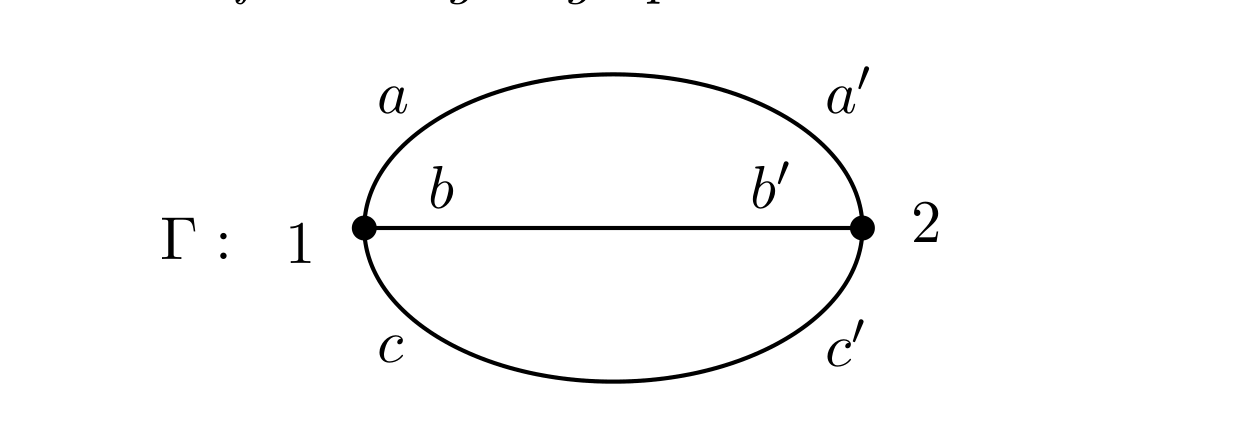
\includegraphics[width=0.50\linewidth]{fig_p035_1.png}
  \caption*{$\Theta$ 图（原文 PDF p.35 示意图，原文无编号）}
\end{figure}
  这里 $V=\{1,2\}$，$HE=\{a,b,c,a',b',c'\}$，$E=\{(a,a'),(b,b'),(c,c')\}$。关联映射为
  \[
    \begin{aligned}
      i_\Gamma:\ HE&\longrightarrow V,\\
      \{a,b,c\}&\longmapsto 1,\\
      \{a',b',c'\}&\longmapsto 2.
    \end{aligned}
  \]
  顶点 $1$ 与 $2$ 的价都是 $3$。
\end{wexam}

\begin{wdefn}{5.6}
  两张图 $\Gamma$ 与 $\Gamma'$ 之间的\textbf{图同构}是一对双射
  \[
    \sigma_V:\ V(\Gamma)\longrightarrow V(\Gamma'),\qquad
    \sigma_{HE}:\ HE(\Gamma)\longrightarrow HE(\Gamma'),
  \]
  它们与关联映射相容（即下图交换）
\begin{figure}[htbp]
  \centering
  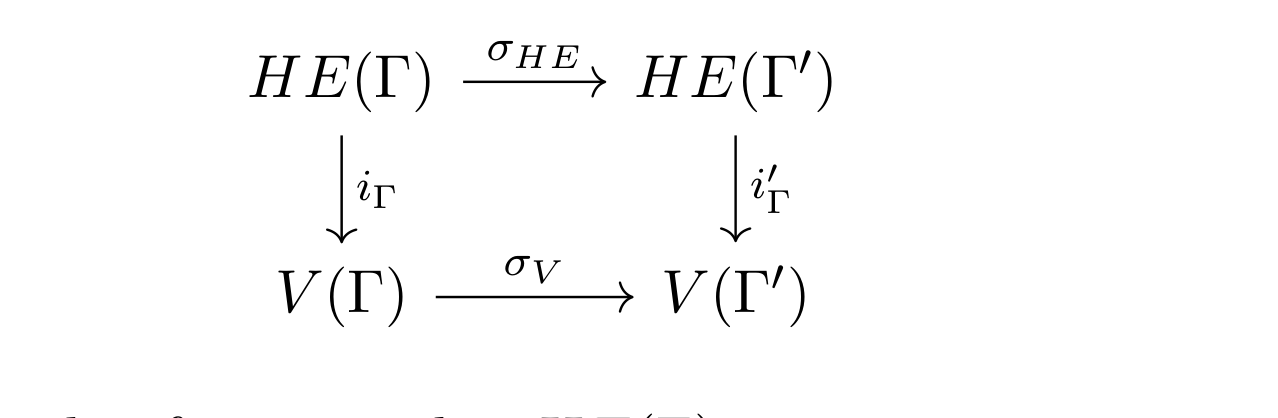
\includegraphics[width=0.51\linewidth]{fig_p035_2.png}
  \caption*{图同构的交换图（原文 PDF p.35 示意图，原文无编号）}
\end{figure}
  并且与边相容：对任意 $a,b\in HE(\Gamma)$，
  \[
    (a,b)\in E(\Gamma)
    \iff
    (\sigma_{HE}(a),\sigma_{HE}(b))\in E(\Gamma').
  \]
  $\Gamma$ 的\textbf{自同构}（automorphism）是一个同构 $\sigma:\Gamma\to\Gamma$。记
  \[
    \Aut(\Gamma)=\Gamma\ \text{的自同构群}.
  \]
\end{wdefn}

% [Tutor Note: 同构的定义要求 $\sigma_V$ 与 $\sigma_{HE}$ 同时给出、且与“哪些半边
% 粘在哪个顶点”以及“哪些半边配成边”两套结构都相容。计算 $\Aut(\Gamma)$ 时最容易
% 只数顶点置换而忘了半边/边的置换（或反之）；正确做法是先固定顶点置换，再看
% 它能延拓出多少半边置换。这个群的阶 $|\Aut(\Gamma)|$ 就是 Feynman 规则中的
% “对称因子”，其倒数 $1/|\Aut(\Gamma)|$ 是本节的核心。]

% >>> p036
\begin{wexam}{5.7}
  考虑
\begin{figure}[htbp]
  \centering
  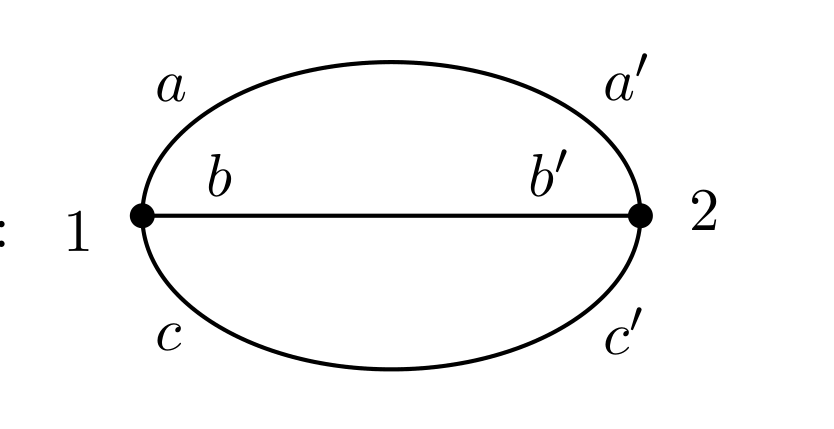
\includegraphics[width=0.33\linewidth]{fig_p036_1.png}
  \caption*{$\Theta$ 图（例 5.7）（原文 PDF p.36 示意图，原文无编号）}
\end{figure}
  这里 $HE=\{a,b,c,a',b',c'\}$，$V=\{1,2\}$，$E=\{(a,a'),(b,b'),(c,c')\}$。
  关联映射同上。下面是 $\Gamma$ 的两个自同构的例子：
  \begin{itemize}[leftmargin=1.6em,itemsep=0.25em]
    \item ① $\sigma_V:(1,2)\mapsto(2,1)$，
          $\sigma_{HE}:(a,b,c,a',b',c')\mapsto(a',b',c',a,b,c)$；
    \item ② $\sigma_V:(1,2)\mapsto(1,2)$，
          $\sigma_{HE}:(a,b,c,a',b',c')\mapsto(b,c,a,b',c',a')$。
  \end{itemize}
  类似地可得 $\Aut(\Gamma)=\Z_2\times S_3$。这里 $\Z_2$ 对应两个顶点的置换，
  $S_3$ 对应三条边的置换。
\end{wexam}

\begin{wexam}{5.8}
  考虑
\begin{figure}[htbp]
  \centering
  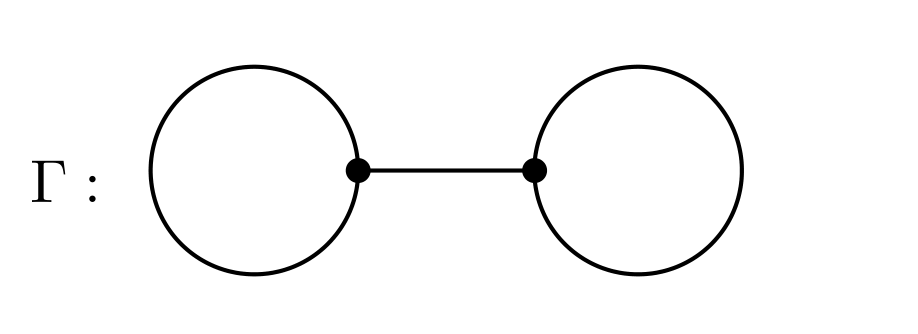
\includegraphics[width=0.37\linewidth]{fig_p036_2.png}
  \caption*{双圈图（原文 PDF p.36 示意图，原文无编号）}
\end{figure}
  可得 $\Aut(\Gamma)=\Z_2\times\Z_2\times\Z_2$。
\end{wexam}

现在让我们考虑
\[
  \langle I(x)^{m}\rangle_x
  =\Bigl\langle\underbrace{I(x)I(x)\cdots I(x)}_{m}\Bigr\rangle_x
\]
的计算。每个 $I(x)$ 给出一个带三条半边的顶点：
\begin{figure}[htbp]
  \centering
  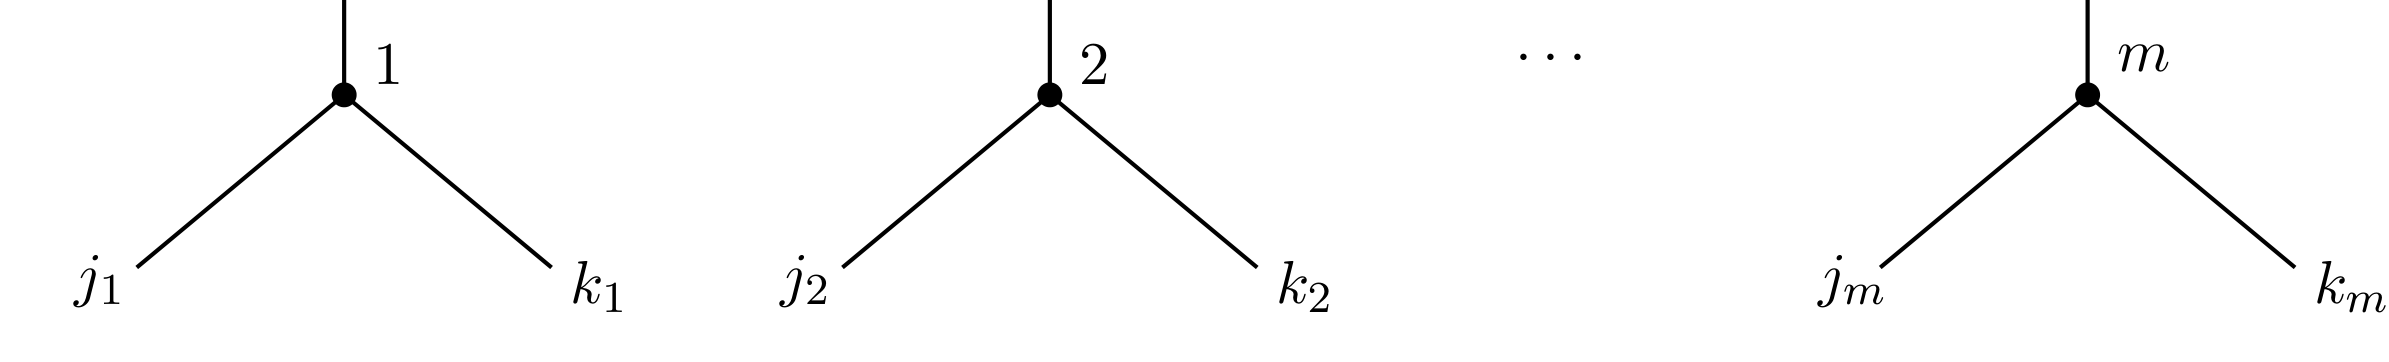
\includegraphics[width=0.92\linewidth]{fig_p036_3.png}
  \caption*{三价顶点及其半边（原文 PDF p.36 示意图，原文无编号）}
\end{figure}
\[
  \begin{aligned}
    &\text{顶点集} && V=\{1,2,\cdots,m\},\\
    &\text{半边集} && HE=\{i_1,j_1,k_1,i_2,j_2,k_2,\cdots,i_m,j_m,k_m\},\\
    &\text{关联映射} && i:\{i_s,j_s,k_s\}\longmapsto\{s\}.
  \end{aligned}
\]
由 Wick 定理，$\langle I(x)^{m}\rangle_x$ 是对完美匹配 $E$ 的一个求和：
\[
  \langle I(x)^{m}\rangle_x
  =\sum_{E\in Y}\hbar^{|E(\Gamma_E)|}\,\omega_{\Gamma_E}.
\]
这里 $Y=\{HE\text{ 的完美匹配}\}$，而 $\Gamma_E$ 是把配对 $E$ 赋给顶点集 $V$ 与半边集
$HE$ 所得到的图。
对每张图 $\Gamma$，$\omega_\Gamma$ 是按照如下赋值得到的数：

% >>> p037
\begin{figure}[htbp]
  \centering
  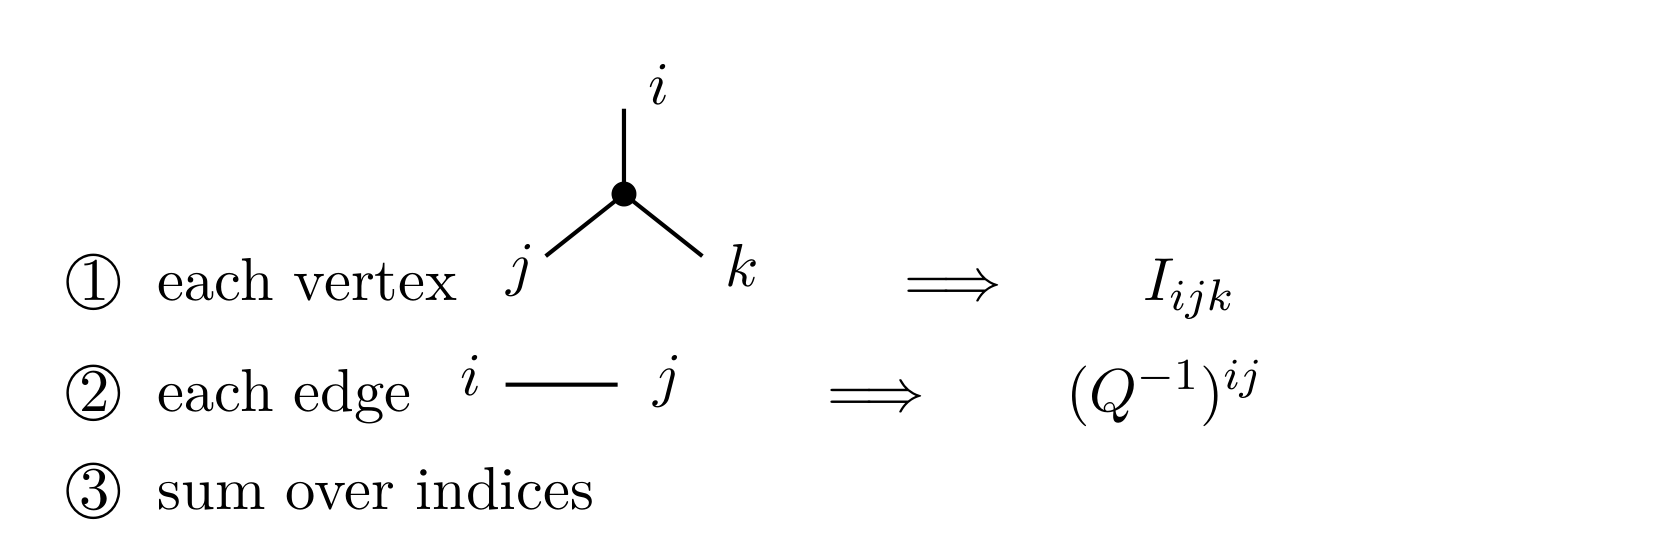
\includegraphics[width=0.67\linewidth]{fig_p037_1.png}
  \caption*{图的赋值规则（原文 PDF p.37 示意图，原文无编号）}
\end{figure}
\begin{itemize}[leftmargin=1.6em,itemsep=0.25em]
  \item ① 每个顶点（三价顶点，三条外线标 $i,j,k$）$\ \Longrightarrow\ I_{ijk}$；
  \item ② 每条边（线段，两端标 $i,j$）$\ \Longrightarrow\ (Q^{-1})^{ij}$；
  \item ③ 对指标求和。
\end{itemize}

\begin{wexam}{5.9}
  考虑
\begin{figure}[htbp]
  \centering
  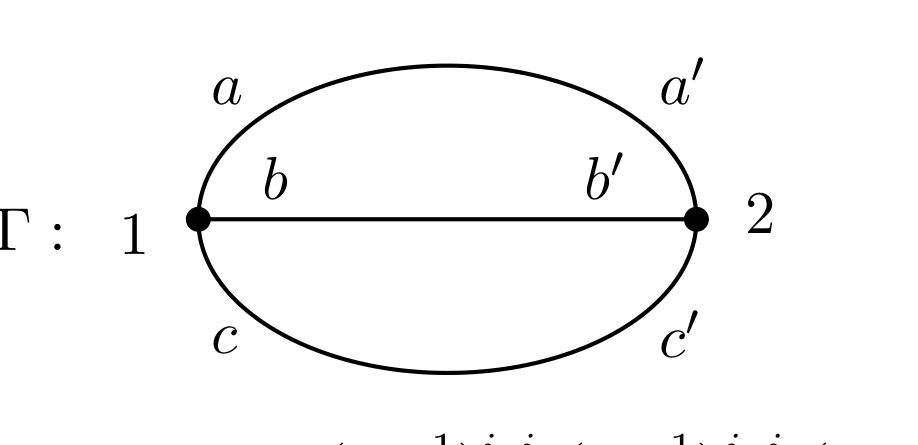
\includegraphics[width=0.37\linewidth]{fig_p037_2.png}
  \caption*{$\Theta$ 图的权（原文 PDF p.37 示意图，原文无编号）}
\end{figure}
  \[
    \omega_\Gamma
    =\sum_{\substack{i_1,j_1,k_1\\ i_2,j_2,k_2}}
    I_{i_1j_1k_1}I_{i_2j_2k_2}
    (Q^{-1})^{i_1i_2}(Q^{-1})^{j_1j_2}(Q^{-1})^{k_1k_2}.
  \]
\end{wexam}

显然，若 $\Gamma$ 与 $\Gamma'$ 同构，则
\[
  \omega_\Gamma=\omega_{\Gamma'}.
\]
这里所有的图都是三价的（每个顶点的价都是 $3$）。保持关联映射的双射
\[
  \sigma_V:V\longrightarrow V,\qquad
  \sigma_{HE}:HE\longrightarrow HE
\]
构成的集合是
\[
  G=\underbrace{S_m}_{\text{置换顶点}}\times
  \underbrace{(S_3)^{m}}_{\text{置换半边}}.
\]
$G$ 在 $Y$ 上有自然的作用，其轨道为
\[
  Y/G=\{\text{由 }m\text{ 个顶点构成的三价图的同构类}\}.
\]
于是
\[
  \begin{aligned}
    \frac{1}{m!(3!)^{m}}\langle I(x)^{m}\rangle_x
    &=\frac{1}{|G|}\sum_{\Gamma\in Y/G}\frac{|G|}{|\Aut(\Gamma)|}
    \,\omega_\Gamma\,\hbar^{|E(\Gamma)|}\\
    &=\sum_{\substack{\Gamma:\text{ 三价图}\\ \text{含 }m\text{ 个顶点}}}
    \frac{\omega_\Gamma}{|\Aut(\Gamma)|}\,\hbar^{|E(\Gamma)|}.
  \end{aligned}
\]
我们还可以把不连通的图按连通同构类归并，从而细化为下面的 Feynman 图展开公式
（细节留给读者）。

% [Tutor Note: 这一段的“除以 $|\Aut(\Gamma)|$”是全节最易错的地方，来龙去脉是：
% 左边 $\frac{1}{m!(3!)^m}$ 把 $m$ 个顶点与每个顶点的 $3!$ 种半边编号都除掉；
% 右边用轨道–稳定子公式 $\sum_{\Gamma\in Y/G}\frac{|G|}{|\Aut|}=|Y|$（更准确地说，
% 每个轨道上的求和给出 $|G|/|\Aut(\Gamma)|$ 个代表），于是 $\frac{1}{|G|}$ 与
% $|G|$ 相消，剩下 $\sum_{\Gamma}\omega_\Gamma/|\Aut(\Gamma)|$。记忆口诀：
% **每张图的权 = 拓扑赋值 $\times$ 耦合常数 $\times\hbar$ 幂 $\div$ 自同构群阶**。
% 对 $\Theta$ 图，$|\Aut|=2\cdot 6=12$，漏掉它会使结果大 $12$ 倍。]

\begin{wprop}{5.10}（Feynman 图展开公式，Feynman Graph Expansion Formula）
  对渐近幂级数，我们有如下的组合图展开公式
  \[
    \begin{aligned}
      \Bigl\langle \ee^{\frac{\lambda}{3!\hbar}I(x)}\Bigr\rangle_x
      &{}:=\sum_{m=0}^{\infty}\frac{\lambda^{m}}{m!\hbar^{m}}
      \left\langle\left(\frac{1}{3!}I(x)\right)^{m}\right\rangle_x\\
      &=\sum_{\Gamma:\ \text{三价}}
      \hbar^{|E(\Gamma)|-|V(\Gamma)|}\lambda^{|V(\Gamma)|}
      \frac{\omega_\Gamma}{|\Aut(\Gamma)|}\\
      &=\exp\left(
      \sum_{\substack{\Gamma:\text{ 连通}\\ \text{三价}}}
      \lambda^{|V(\Gamma)|}\hbar^{l(\Gamma)-1}
      \frac{\omega_\Gamma}{|\Aut(\Gamma)|}
      \right).
    \end{aligned}
  \]
\end{wprop}

% [Tutor Note: 命题 5.10 中的等号应理解为**渐近展开**意义下的等式（原文在 p.38 用
% $e^{\cdots}\stackrel{\text{asymptotic}}{=}\exp(\cdots)$ 强调），不是收敛级数的恒等式。
% 最后一步“不连通图之和取指数”是标准的指数公式
% （exponential formula）：任何一张图唯一分解为若干连通图的无序并，
% 而 $\exp$ 的 Taylor 系数中 $\frac{1}{k!}$ 恰好负责“无序”。这里的 $k!$ 与
% $|\Aut|$ 的配合是本段的技术核心。]

% >>> p038
这里对连通图 $\Gamma$，
\[
  l(\Gamma)=|E(\Gamma)|-|V(\Gamma)|+1=1-\chi(\Gamma)
\]
称为 $\Gamma$ 的\textbf{圈数}（loop number）。
\begin{figure}[htbp]
  \centering
  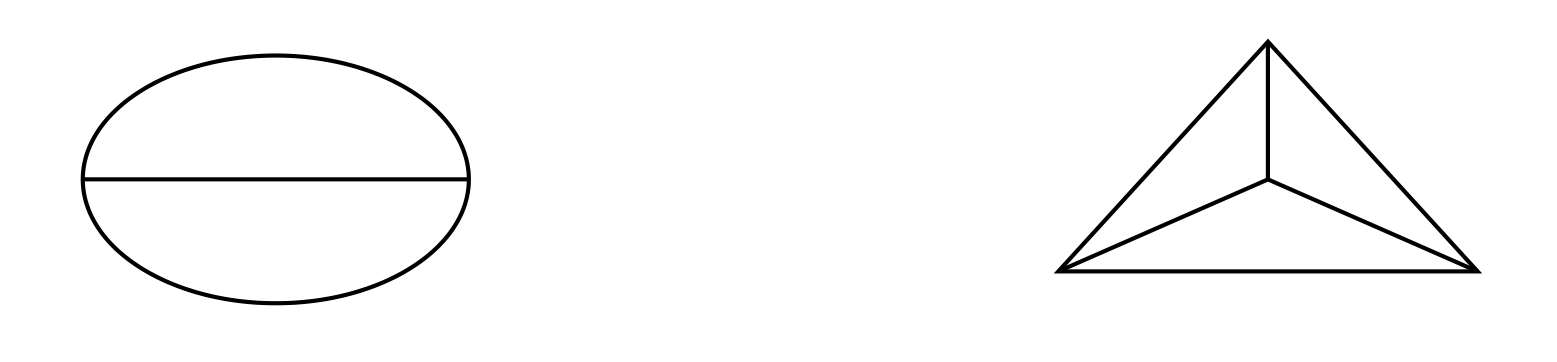
\includegraphics[width=0.62\linewidth]{fig_p038_1.png}
  \caption*{圈数的两个例子（原文 PDF p.38 示意图，原文无编号）}
\end{figure}
\[
  l(\Gamma)=3-2+1=2
  \qquad\qquad
  l(\Gamma)=6-4+1=3
\]
一般而言，如果相互作用包含所有可能次数的项
\[
  \frac{\lambda_3}{3!}I_3(x)+\frac{\lambda_4}{4!}I_4(x)
  +\cdots+\frac{\lambda_m}{m!}I_m(x)+\cdots,
\]
那么级数展开将包含所有可能的图，其中每个价为 $m$ 的顶点都类似地赋予值 $I_m$。
一般的 Feynman 图展开公式为
\[
  \Bigl\langle
  \ee^{\frac{1}{\hbar}\left(\sum_{m\ge3}\frac{\lambda_m}{m!}I_m(x)\right)}
  \Bigr\rangle_x
  \overset{\text{asymptotic}}{=}
  \exp\left(
  \sum_{\substack{\Gamma:\text{ 连通}\\\text{图}}}
  \Bigl(\prod_{m\ge3}\lambda_m^{|V_m(\Gamma)|}\Bigr)
  \hbar^{l(\Gamma)-1}\frac{\omega_\Gamma}{|\Aut(\Gamma)|}
  \right),
\]
其中 $V_m(\Gamma)$ 是价为 $m$ 的顶点的集合。

% [Tutor Note: 圈数公式的两种写法 $l=|E|-|V|+1=1-\chi$ 只有在 $\Gamma$ **连通**时
% 才相等（$\chi=|V|-|E|$ 对连通图成立）；对不连通图应以 $|E|-|V|+c$ 为准，
% 其中 $c$ 是连通分支数。原文此处已声明 “for a connected graph”，引用时勿丢。
% 另外 $\hbar^{l-1}$ 的幂次是“圈数减一”：树图（$l=0$）给 $\hbar^{-1}$，
% 与整体归一化相消，这是半经典展开的体现。]

\subsection{Green 函数（Green's Function）}

现在讨论无穷维情形。为说明基本想法，让我们考虑标量场论，其场空间为
$\mathcal E=C_c^{\infty}(\R^d)$，作用量泛函为
\[
  S[\phi]=\frac{1}{2}\int_{\R^d}\Bigl(\sum_i(\partial_i\phi)^2
  +m^2\phi^2\Bigr)\dd x^d,
  \qquad \phi\in\mathcal E.
\]
我们关心的是关联函数（correlation function）
\[
  \langle\mathcal O\rangle
  =\frac{\displaystyle\int_{\mathcal E}[\mathcal D\phi]\,
  \ee^{-\frac{1}{\hbar}S[\phi]}\mathcal O(\phi)}
  {\displaystyle\int_{\mathcal E}[\mathcal D\phi]\,
  \ee^{-\frac{1}{\hbar}S[\phi]}},
\]
其中 $\mathcal O$ 是 $\mathcal E$ 上的函数，称为\textbf{可观测量}（observable）。
例如我们想计算
\[
  \langle\phi(y_1)\cdots\phi(y_{2s})\rangle,
  \qquad\text{其中 } y_i\in\R^d.
\]
尽管对这种无穷维积分我们没有一般的测度理论，我们仍可以模仿有限维情形，
得到一个组合式的预期结果。让我们写成
\[
  S[\phi]=\frac{1}{2}\int_{\R^d}\phi D\phi\,\dd x^d,
\]
其中
\[
  D=-\sum_{i=1}^{d}\frac{\partial^{2}}{\partial x^{i}\partial x^{i}}+m^{2}.
\]

% >>> p039
这是 $\phi$ 的二次型，类似于高斯积分中的 $Q(x)$。确切地说，我们可以把有限维与
无穷维情形作如下对照：
\begin{center}
  \begin{tabular}{cc}
    \toprule
    \textbf{有限维情形} & \textbf{无穷维情形}\\
    \midrule
    $\R^{n}$ & $\mathcal E=C_c^{\infty}(\R^{d})$\\
    $x^{i}$ & $\phi(x)$\\
    $i$ & 一个点 $x\in\R^{d}$\\
    $\sum_{i}$ & $\int_{\R^{d}}\dd x$\\
    $\frac{1}{2}Q(x)=\frac{1}{2}\sum_{i,j}Q_{ij}x^{i}x^{j}$
      & $S[\phi]=\frac{1}{2}\int\phi D\phi$\\
    $\langle x^{i}x^{j}\rangle=(A^{-1})^{ij}$
      & $\langle\phi(x)\phi(y)\rangle=G(x,y)$\\
    $\delta_{ij}$ & $\delta(x-y)$\\
    \bottomrule
  \end{tabular}
\end{center}

% [Tutor Note: 对照表中有两处原书的不一致，引用时请留意：（i）左栏写的是
% $(A^{-1})^{ij}$，而本节前文一直用 $(Q^{-1})^{ij}$，应读作同一逆矩阵；
% （ii）表右栏只写 $S[\phi]=\frac12\int\phi D\phi$，漏了测度 $\dd x^d$
% （前文公式是带 $\dd x^d$ 的）。这两处均照录原文。表中“$\sum_i\leftrightarrow\int$”
% 一行说明有限维与无穷维的唯一差别是把求和换成积分——Wick 定理的组合结构完全不变。]

函数 $G(x,y)$ 表示 $D$ 关于 $x$ 的逆：
\[
  D_xG(x,y)=\delta(x-y).
\]
事实上，若对光滑函数 $f$ 定义如下算子
\[
  (Gf)(x)=\int\dd y\,G(x,y)f(y),
\]
则
\[
  \begin{aligned}
    D(Gf)(x)&=\int\dd y\,D_xG(x,y)f(y)\\
    &=\int\dd y\,\delta(x-y)f(y)=f(x).
  \end{aligned}
\]
这样的函数存在，称为\textbf{Green 函数}。

\begin{wexam}{5.11}
  考虑 $\R^d$ 上的标准 Laplacian
  $D=-\sum_i\frac{\partial^2}{\partial x^i\partial x^i}$。当 $d\ge3$ 时，
  Green 函数具有如下形式
  \[
    G(x,y)\propto\frac{1}{\|x-y\|^{d-2}}.
  \]
  特别地，当 $x\to y$ 时 $G(x,y)$ 变得奇异。这反映了无穷维的本质，
  也是量子场论中“\textbf{UV 发散}”（紫外发散）的根源。
\end{wexam}

% [Tutor Note: 例 5.11 只写了比例关系 $\propto$；精确常数是
% $G(x,y)=\frac{1}{(d-2)\Omega_{d-1}}\|x-y\|^{-(d-2)}$，其中 $\Omega_{d-1}$
% 是单位球面面积。注意 $d=1,2$ 时形式不同（$d=2$ 是对数），所以“$d\ge3$”不可省。
% 对角 $x=y$ 处的奇点就是后面 UV 发散的来源：图积分沿对角方向发散，
% 需靠重整化（part06）处理。]

我们用 Wick 定理来计算
\[
  \langle\phi(y_1)\cdots\phi(y_{2s})\rangle
  =\hbar^{s}\sum_{\sigma\in P(2s)}
  G(y_{\sigma(1)},y_{\sigma(2)})G(y_{\sigma(3)},y_{\sigma(4)})\cdots
  G(y_{\sigma(2s-1)},y_{\sigma(2s)}),
\]
它可以形象化为对完美配对的求和。每条从 $y$ 到 $z$ 的边代表 Green 函数 $G(y,z)$，
它扮演传播子的角色。
\begin{figure}[htbp]
  \centering
  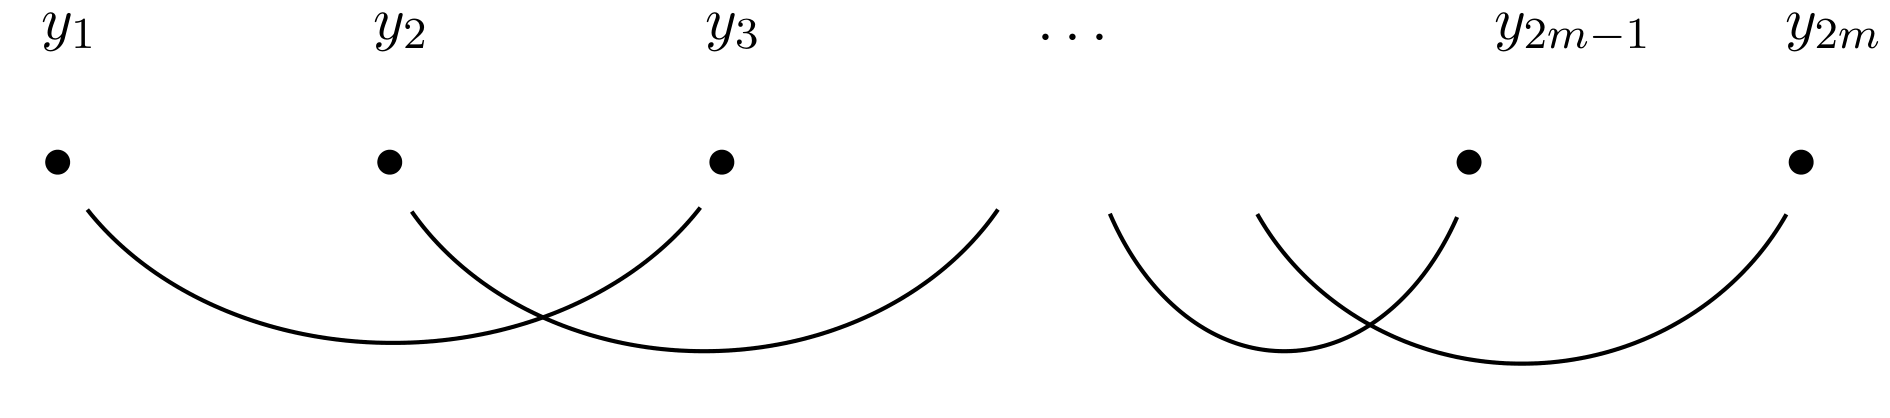
\includegraphics[width=0.76\linewidth]{fig_p039_1.png}
  \caption*{无穷维情形的配对图（原文 PDF p.39 示意图，原文无编号）}
\end{figure}

% [Tutor Note: 与有限维 Wick 定理逐项对应：$\langle x^{i}x^{j}\rangle
% =\hbar(Q^{-1})^{ij}$ 换成 $\langle\phi(x)\phi(y)\rangle=\hbar G(x,y)$，
% 而 $2s$ 个场配成 $s$ 对给出总因子 $\hbar^{s}$。原文在这一段混用了 $2s$（公式）
% 与 $2m$（图注、下文），实为同一整数；本译本照录。还要注意符号约定：
% 作用量写成 $e^{-S/\hbar}$（Euclidean 号差），而 p.31 的路径积分写成
% $e^{iS/\hbar}$（Minkowski）——两处约定不同，是常见混淆点，Wick 转动即联系二者。]

% >>> p040
现在我们可以进而考虑有相互作用的理论。例如，我们可以通过给 $S$ 加上如下项
\[
  I_3(\phi)=\frac{\lambda}{3!}\int\phi^{3}
\]
来考虑 $\phi^{3}$ 理论，或者通过加上
\[
  I_4(\phi)=\frac{\lambda}{4!}\int\phi^{4}
\]
来考虑 $\phi^{4}$ 理论。

我们将有类似的 Feynman 图展开。下面是两个三价图的例子以及它们所代表的积分。
\begin{figure}[htbp]
  \centering
  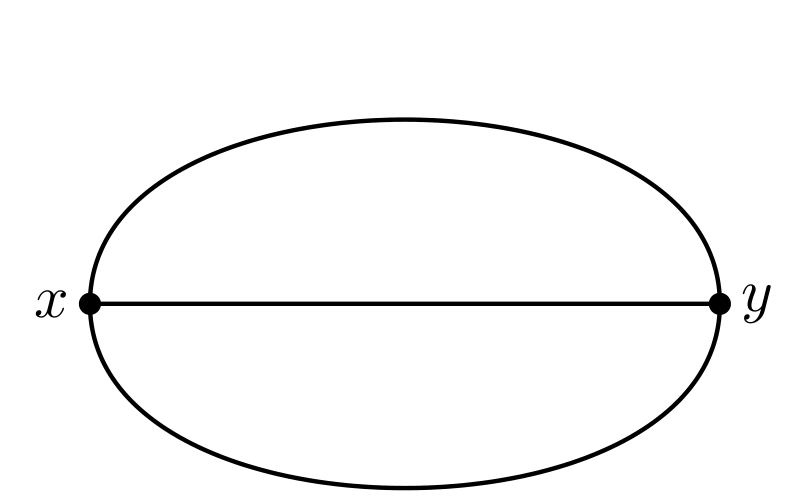
\includegraphics[width=0.32\linewidth]{fig_p040_1.png}
  \caption*{三价图及其积分（一）（原文 PDF p.40 示意图，原文无编号）}
\end{figure}
\[
  \int_{(\R^{d})^{2}}\dd x\,\dd y\,G(x,y)^{3}
\]
\begin{figure}[htbp]
  \centering
  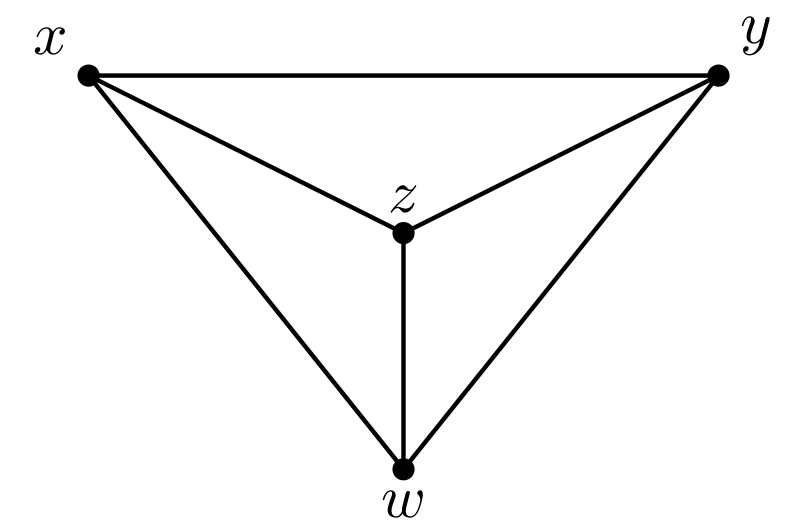
\includegraphics[width=0.32\linewidth]{fig_p040_2.png}
  \caption*{三价图及其积分（二）（原文 PDF p.40 示意图，原文无编号）}
\end{figure}
\[
  \int_{(\R^{d})^{4}}\dd x\,\dd y\,\dd z\,\dd w\,
  G(x,y)G(y,w)G(w,x)G(x,z)G(y,z)G(w,z)
\]
然而，由于 $G(x,y)$ 在对角上的奇异性，这样的图积分一般是发散的。这就是
\textbf{UV 发散}。“\textbf{重整化理论}”（renormalization theory）研究如何处理
这种发散以得到有意义的有限答案。

\subsection{正则量子化（Canonical Quantization）}

在一般地研究 UV 发散之前，让我们先理解这样的考虑如何导向量子力学中的正则量子化。

考虑相空间 $\R^{2}$ 上的力学，其坐标为 $(x,p)$，辛形式为 $\omega=\dd x\wedge\dd p$。
经典地，相空间上的函数集合带有由下式定义的 Poisson 结构 $\{-,-\}$：
\[
  \{f(x,p),g(x,p)\}
  =\frac{\partial f}{\partial x}\frac{\partial g}{\partial p}
  -\frac{\partial f}{\partial p}\frac{\partial g}{\partial x}.
\]
量子力学地，$x$ 与 $p$ 被量子化为算符 $\hat x$ 与 $\hat p$，满足正则对易关系
\[
  [\hat x,\hat p]=\ii\hbar .
\]


% ---------- part06.tex ----------
% ============================================================
%  part06.tex  |  原文 PDF p.41–47（页脚 p.40–46）
%  内容：第 5 章 微扰展开（续）
%        5.4 正则量子化（Canonical Quantization）—— 续文
%        5.5 抵消项与重整化（Counter-term and Renormalization）
%  分节说明：5.4 的 \subsection 标题位于 PDF p40 下半页，由 part05 提供；
%            本片段从 p41 的 5.4 续文开始，故不重复 5.4 标题；
%            5.5 的 \subsection 标题起于 PDF p45，见下文。
% ============================================================

% >>> p041

代数上，我们可以把它看作相空间上函数环 $A$ 的形变。记
$A^{\hbar}=A[\hbar]$ 为带有形变乘法 $*$ 的形变环，该乘法称为\emph{Moyal 积}。
对 $f,g\in A$，有（在 $\hbar$ 的渐近意义下）
\[
  \begin{aligned}
    f(x,p)*g(x,p)
    &=f(x,p)\,\ee^{\frac{\ii\hbar}{2}\left(
        \overleftarrow{\frac{\partial}{\partial x}}
        \overrightarrow{\frac{\partial}{\partial p}}
        -\overleftarrow{\frac{\partial}{\partial p}}
        \overrightarrow{\frac{\partial}{\partial x}}
      \right)}g(x,p)\\
    &=f(x,p)g(x,p)+\frac{\ii\hbar}{2}\{f,g\}+O(\hbar^2).
  \end{aligned}
\]
可以验证：
\textcircled{1}\ $*$ 是结合的：
\[
  f*(g*h)=(f*g)*h,\qquad \forall f,g,h\in A;
\]
\textcircled{2}\ 正则对易关系成立：
\[
  [x,p]_*=x*p-p*x=\ii\hbar.
\]

% [Tutor Note: Moyal 积指数中左右箭头的方向约定极易出错。原文是
% $\overleftarrow{\partial_x}\overrightarrow{\partial_p}-\overleftarrow{\partial_p}
% \overrightarrow{\partial_x}$：左箭头表示该导数作用在左边的 $f$ 上，右箭头表示作用在
% 右边的 $g$ 上。若把两项的次序写反，则一次项 $\{f,g\}$ 整体变号，与后面的
% $\{f,g\}=\partial_x f\,\partial_p g-\partial_p f\,\partial_x g$ 不再匹配。
% 校对时请核对原书 p.40 / PDF p.41。]

Moyal 积 $*$ 有如下 Feynman 图解释。引入两个描述相空间 $\R^2$ 上力学的场
\[
  \gamma(t)=\left(\mathbb{X}(t),\mathbb{P}(t)\right):\ \R_t\longrightarrow\R^2,
\]
并考虑自由作用量
\[
  S_0[\gamma]=\int_{\R}\mathbb{P}(t)\dd\mathbb{X}(t)
  =\int_{\R}\mathbb{P}(t)\dot{\mathbb{X}}(t)\dd t
  =\int_{\R}\mathbb{P}(t)\frac{\dd}{\dd t}\mathbb{X}(t).
\]
我们关心可观测量 $\mathbb{O}$ 的期望
\[
  \langle\mathbb{O}\rangle
  =\frac{\int[D\gamma]\,\ee^{\frac{\ii}{\hbar}S_0[\gamma]}\,\mathbb{O}(\gamma)}
        {\int[D\gamma]\,\ee^{\frac{\ii}{\hbar}S[\gamma]}}.
\]

% [Tutor Note: 上式的分母指数中原文写的是 $S[\gamma]$，而分子中写的是自由作用量
% $S_0[\gamma]$；按上下文（自由理论的期望）分母也应为 $S_0[\gamma]$，此处疑为原文
% 笔误。按体例照录原文，请核对原书 p.40 / PDF p.41。]

让我们写出（暂时忽略边界行为）
\[
  \begin{aligned}
    S_0[\gamma]
    &=\frac{1}{2}\int\left(\mathbb{P}\dot{\mathbb{X}}-\mathbb{X}\dot{\mathbb{P}}\right)\dd t\\
    &=\frac{1}{2}\int
      \begin{bmatrix}\mathbb{X}&\mathbb{P}\end{bmatrix}
      \begin{bmatrix}0&-\frac{\dd}{\dd t}\\[2pt]\frac{\dd}{\dd t}&0\end{bmatrix}
      \begin{bmatrix}\mathbb{X}\\[2pt]\mathbb{P}\end{bmatrix}\dd t.
  \end{aligned}
\]
因此
\[
  \ee^{\frac{\ii}{\hbar}S_0[\gamma]}
  =\exp\left(-\frac{1}{2\hbar}\left(
    \frac{1}{\ii}\int
    \begin{bmatrix}\mathbb{X}(t)&\mathbb{P}(t)\end{bmatrix}
    \begin{bmatrix}0&-\frac{\dd}{\dd t}\\[2pt]\frac{\dd}{\dd t}&0\end{bmatrix}
    \begin{bmatrix}\mathbb{X}(t)\\[2pt]\mathbb{P}(t)\end{bmatrix}\dd t
  \right)\right).
\]
与有限维情形
\[
  \ee^{-\frac{1}{2\hbar}\sum_{i,j}Q_{ij}x^ix^j}
\]
相比较，逆矩阵 $Q^{-1}$ 的类比物是
\[
  \ii
  \begin{bmatrix}0&-\frac{\dd}{\dd t}\\[2pt]\frac{\dd}{\dd t}&0\end{bmatrix}^{-1}.
\]
$\frac{\dd}{\dd t}$ 的 Green 函数是满足
\[
  \frac{\partial}{\partial t_1}G(t_1,t_2)=\delta(t_1-t_2)
\]
的函数 $G(t_1,t_2)$。

% [Tutor Note: “与有限维高斯积分比较”这一步是把 $\frac{\ii}{\hbar}S_0$ 写成
% $-\frac{1}{2\hbar}\cdot\frac{1}{\ii}\int z^{\mathsf T}Mz$ 的形式，其中
% $z=(\mathbb{X},\mathbb{P})^{\mathsf T}$、$M=\begin{bsmallmatrix}0&-\partial_t\\
% \partial_t&0\end{bsmallmatrix}$；因为 $\frac{1}{\ii}=-\ii$，指数恰为
% $\frac{\ii}{2\hbar}\int z^{\mathsf T}Mz$。这个 $\frac{1}{\ii}$ 因子若漏掉，
% 后面两点函数的 $\ii$ 因子会整体错位。]

% >>> p042

这里 $\delta(t_1-t_2)$ 可以看作 $\delta_{ij}$ 的无穷维类比。用
$G(t_1,t_2)$ 写出，我们有
\[
  \begin{bmatrix}0&-\frac{\partial}{\partial t_1}\\[2pt]
    \frac{\partial}{\partial t_1}&0\end{bmatrix}
  \begin{bmatrix}0&G(t_1,t_2)\\[2pt]-G(t_1,t_2)&0\end{bmatrix}
  =\begin{bmatrix}\delta(t_1-t_2)&0\\[2pt]0&\delta(t_1-t_2)\end{bmatrix}.
\]
右端可以看作无穷维单位矩阵的 $(t_1,t_2)$-元。因此上述逆的 $(t_1,t_2)$-元可以写成
\[
  \ii
  \begin{bmatrix}0&-\frac{\dd}{\dd t}\\[2pt]\frac{\dd}{\dd t}&0\end{bmatrix}^{-1}_{t_1,t_2}
  =\begin{bmatrix}0&\ii G(t_1,t_2)\\[2pt]-\ii G(t_1,t_2)&0\end{bmatrix}.
\]
于是我们可以用这个逆来“定义”两点函数：
\[
  \left\lbrace
  \begin{aligned}
    \langle\mathbb{X}(t_1)\mathbb{P}(t_2)\rangle_\gamma
      &:=\ii\hbar G(t_1,t_2)\\
    \langle\mathbb{P}(t_1)\mathbb{X}(t_2)\rangle_\gamma
      &:=-\ii\hbar G(t_1,t_2)\\
    \langle\mathbb{X}(t_1)\mathbb{X}(t_2)\rangle_\gamma
      &=\langle\mathbb{P}(t_1)\mathbb{P}(t_2)\rangle_\gamma=0
  \end{aligned}
  \right.
\]
我们剩下要解出 $G(t_1,t_2)$。上式要求 $G(t_1,t_2)$ 满足
\[
  G(t_1,t_2)=-G(t_2,t_1).
\]
$\frac{\dd}{\dd t}$ 的这种 Green 函数由下式显式给出
\[
  G(t_1,t_2)=\frac{1}{2}\sgn(t_1-t_2)
  =\begin{cases}
    \frac{1}{2}, & t_1>t_2,\\[2pt]
    0, & t_1=t_2,\\[2pt]
    -\frac{1}{2}, & t_1<t_2.
  \end{cases}
\]
\begin{figure}[htbp]
  \centering
  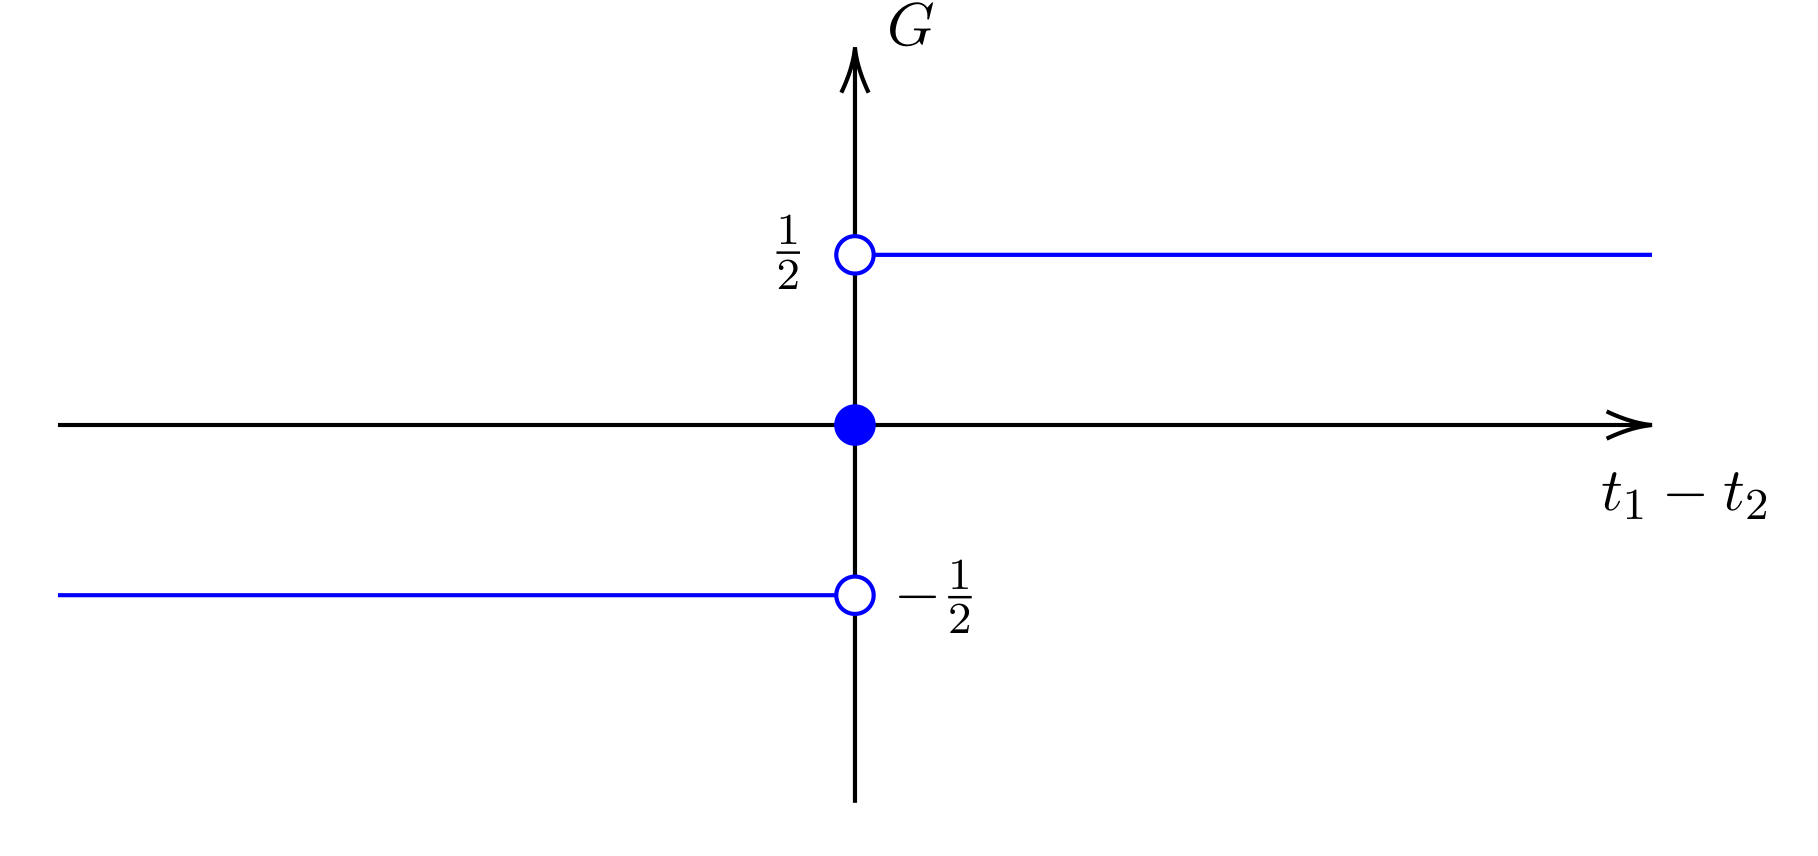
\includegraphics[width=0.73\linewidth]{fig_p042_1.png}
  \caption*{Green 函数 $G(t_1,t_2)=\tfrac12\sgn(t_1-t_2)$ 的图像（原文 PDF p.42 示意图，原文无编号）}
\end{figure}

% [Tutor Note: 这里 $G$ 关于两个时间变量\emph{反对称}，故
% $\langle\mathbb{X}(t_1)\mathbb{P}(t_2)\rangle=-\langle\mathbb{X}(t_2)
% \mathbb{P}(t_1)\rangle$，这正是 $\langle\mathbb{X}\mathbb{P}\rangle$ 与
% $\langle\mathbb{P}\mathbb{X}\rangle$ 相差一个负号的原因（见下一段）。若文献把
% 传播子定义为对称的 $\frac{1}{2}\sgn$ 与 $\frac{\ii\hbar}{2}$ 的组合，请先确认其
% 时间序/编时约定，两种约定在这一点上不可混用。]

事实上，对任意紧支集检验函数 $f(t)$，
\[
  \begin{aligned}
    -\int_{\R}\dd t_1\,G(t_1,t_2)f'(t_1)
    &=\frac{1}{2}\int_{-\infty}^{t_2}\dd t_1\,f'(t_1)
      -\frac{1}{2}\int_{t_2}^{\infty}\dd t_1\,f'(t_1)\\
    &=\frac{1}{2}f(t_2)-\frac{1}{2}\left(-f(t_2)\right)=f(t_2).
  \end{aligned}
\]
因此
\[
  \frac{\partial}{\partial t_1}G(t_1,t_2)=\delta(t_1-t_2)
\]
作为分布意义下的等式成立。

总之，我们关心如下两点函数
\[
  \langle\mathbb{X}(t_1)\mathbb{P}(t_2)\rangle_\gamma\ \text{“=”}\
  \frac{\int[D\gamma]\,\ee^{\frac{\ii}{\hbar}S_0[\gamma]}\,
        \mathbb{X}(t_1)\mathbb{P}(t_2)}
       {\int[D\gamma]\,\ee^{\frac{\ii}{\hbar}S_0[\gamma]}}.
\]

% >>> p043

尽管我们先验地不知道路径积分测度的精确信息，仍可与有限维高斯积分作比较，
得到一个合理的结果
\[
  \langle\mathbb{X}(t_1)\mathbb{P}(t_2)\rangle_\gamma
  :=\ii\hbar G(t_1,t_2)=\frac{\ii\hbar}{2}\sgn(t_1-t_2).
\]
以下我们就用这个公式来定义两点函数。

注意这个两点函数，也就是传播子，不依赖于 $t_1,t_2$ 的精确数值，而只依赖于
它们的相对位置
\[
  \langle\mathbb{X}(t_1)\mathbb{P}(t_2)\rangle_\gamma
  =\begin{cases}
    \frac{\ii\hbar}{2}, & t_1>t_2,\\[2pt]
    0, & t_1=t_2,\\[2pt]
    -\frac{\ii\hbar}{2}, & t_1<t_2.
  \end{cases}
\]
这表明该模型具有拓扑性质——事实上的确如此。

现在设 $f(x,p)$ 与 $g(x,p)$ 是两个多项式。我们在时间轴上把它们画成
\begin{figure}[htbp]
  \centering
  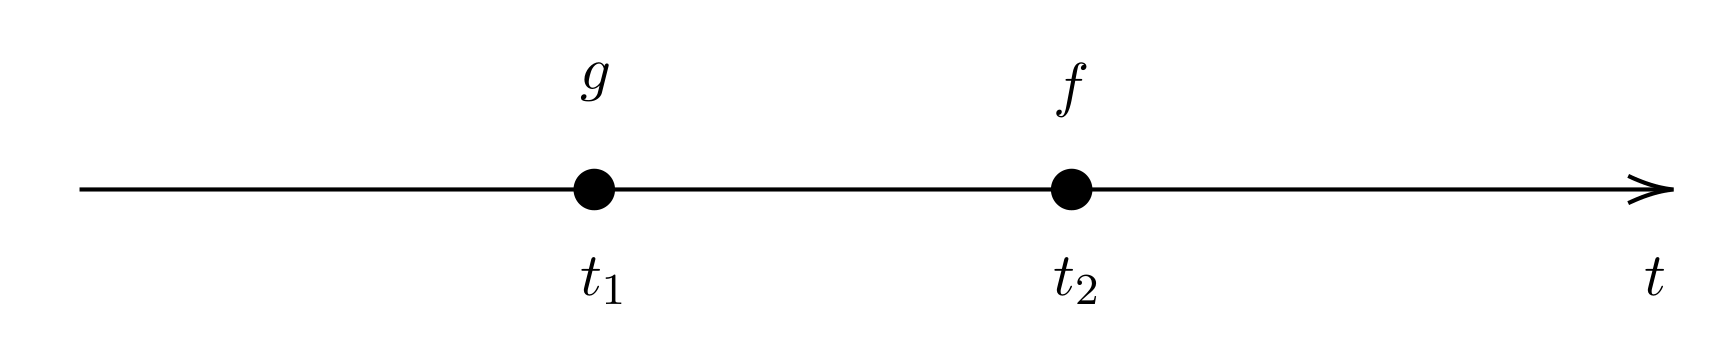
\includegraphics[width=0.69\linewidth]{fig_p043_1.png}
  \caption*{时间轴上的两个算子 $g$ 与 $f$（原文 PDF p.43 示意图，原文无编号）}
\end{figure}
如下形式。我们通过如下关联来定义相空间上的一个新函数
\[
  \langle f(x+\mathbb{X}(t_2),p+\mathbb{P}(t_2))\,
    g(x+\mathbb{X}(t_1),p+\mathbb{P}(t_1))\rangle_\gamma.
\]
这里我们用时刻 $t_1$ 的量子涨落 $\mathbb{X}(t),\mathbb{P}(t)$ 扰动 $g$ 的变量，
用时刻 $t_2$ 的涨落扰动 $f$ 的变量。等价地，可以把 $x,p$ 看作“背景”平移。
这个关联函数依赖于背景变量 $\{x,p\}$，从而定义了相空间上的一个函数。

让我们应用 Wick 定理来计算这个关联。把 $f$ 与 $g$ 各表示为一个顶点，
其价数等于该多项式的次数
\begin{figure}[htbp]
  \centering
  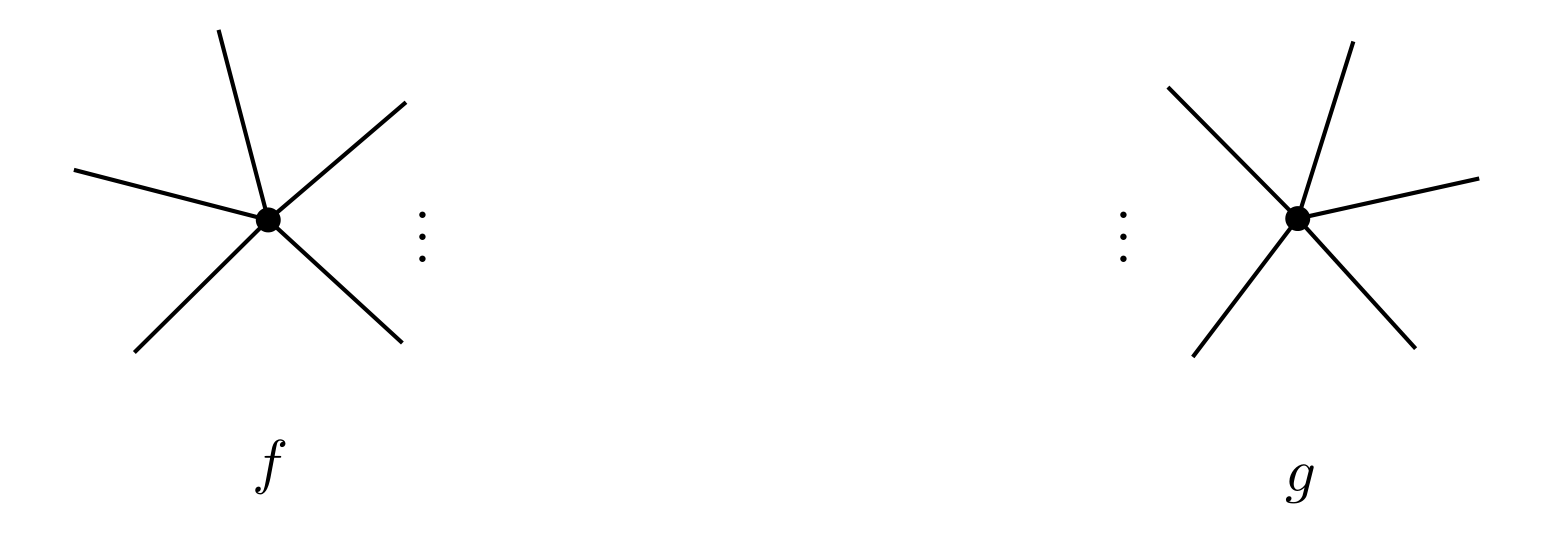
\includegraphics[width=0.62\linewidth]{fig_p043_2.png}
  \caption*{多项式 $f$ 与 $g$ 对应的星形顶点（原文 PDF p.43 示意图，原文无编号）}
\end{figure}
于是 Wick 定理说，该关联等于对所有把 $f$、$g$ 的半边两两配对的方式求和
\begin{figure}[htbp]
  \centering
  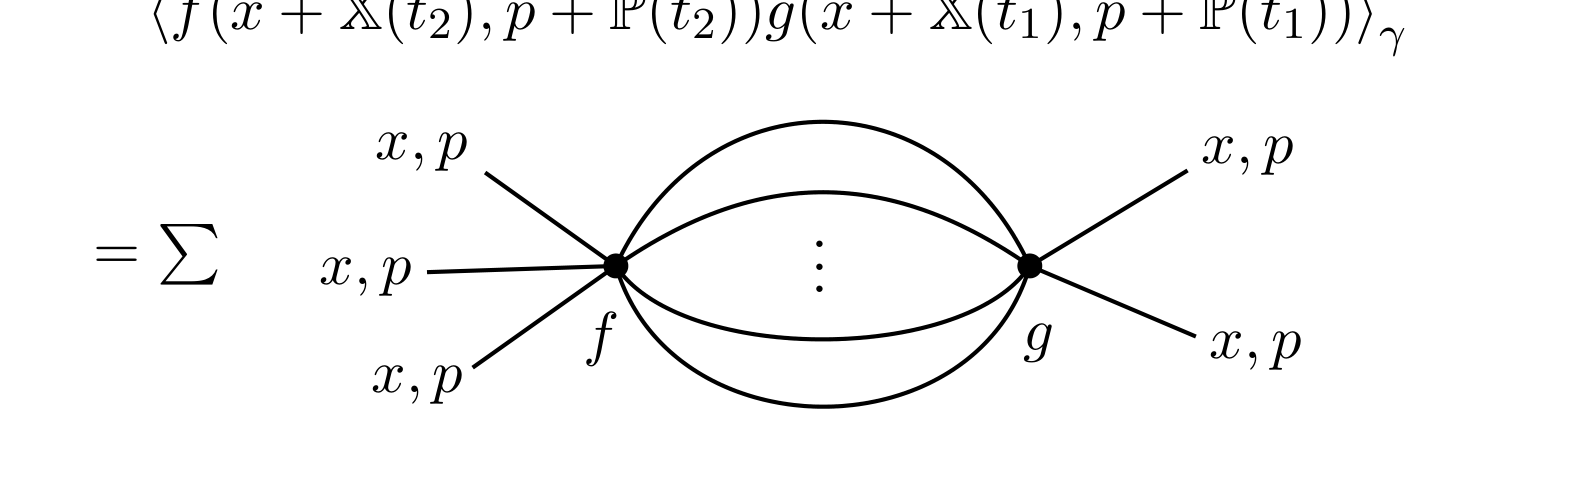
\includegraphics[width=0.64\linewidth]{fig_p043_3.png}
  \caption*{Wick 定理：对全部收缩方式求和（原文 PDF p.43 示意图，原文无编号）}
\end{figure}
这里对每一个未配对的半边，按它在原来顶点中的位置赋以 $x$ 或 $p$；对配对的
半边，

% [Tutor Note: 原文 PDF p.43 中“Wick 定理”那一行是一个\emph{图形公式}
% （左端为关联函数，右端为 $\Sigma$ 加上一张收缩图），不是通常的代数公式。
% 本译本用图标记 + 文字说明等价地保留其内容，未作任何数学上的改写。若需核对，
% 请见原书 p.42 下半页 / PDF p.43。]

% [Tutor Note: 配对时只有 $\langle\mathbb{X}\mathbb{P}\rangle$ 与
% $\langle\mathbb{P}\mathbb{X}\rangle$ 非零，$\langle\mathbb{X}\mathbb{X}\rangle
% =\langle\mathbb{P}\mathbb{P}\rangle=0$（见 PDF p.42 的定义）。因此一条传播子
% 必然连接一个“$x$ 型”半边与一个“$p$ 型”半边；哪些半边算 $x$ 型、哪些算 $p$ 型，
% 由原来顶点 $f,g$ 中该半边所携带的变量决定，这是本段容易看漏的关键。]

% >>> p044

见下图：每一条传播子给出一个因子 $\frac{\ii}{2}\hbar$ 或 $-\frac{\ii}{2}\hbar$
\begin{figure}[htbp]
  \centering
  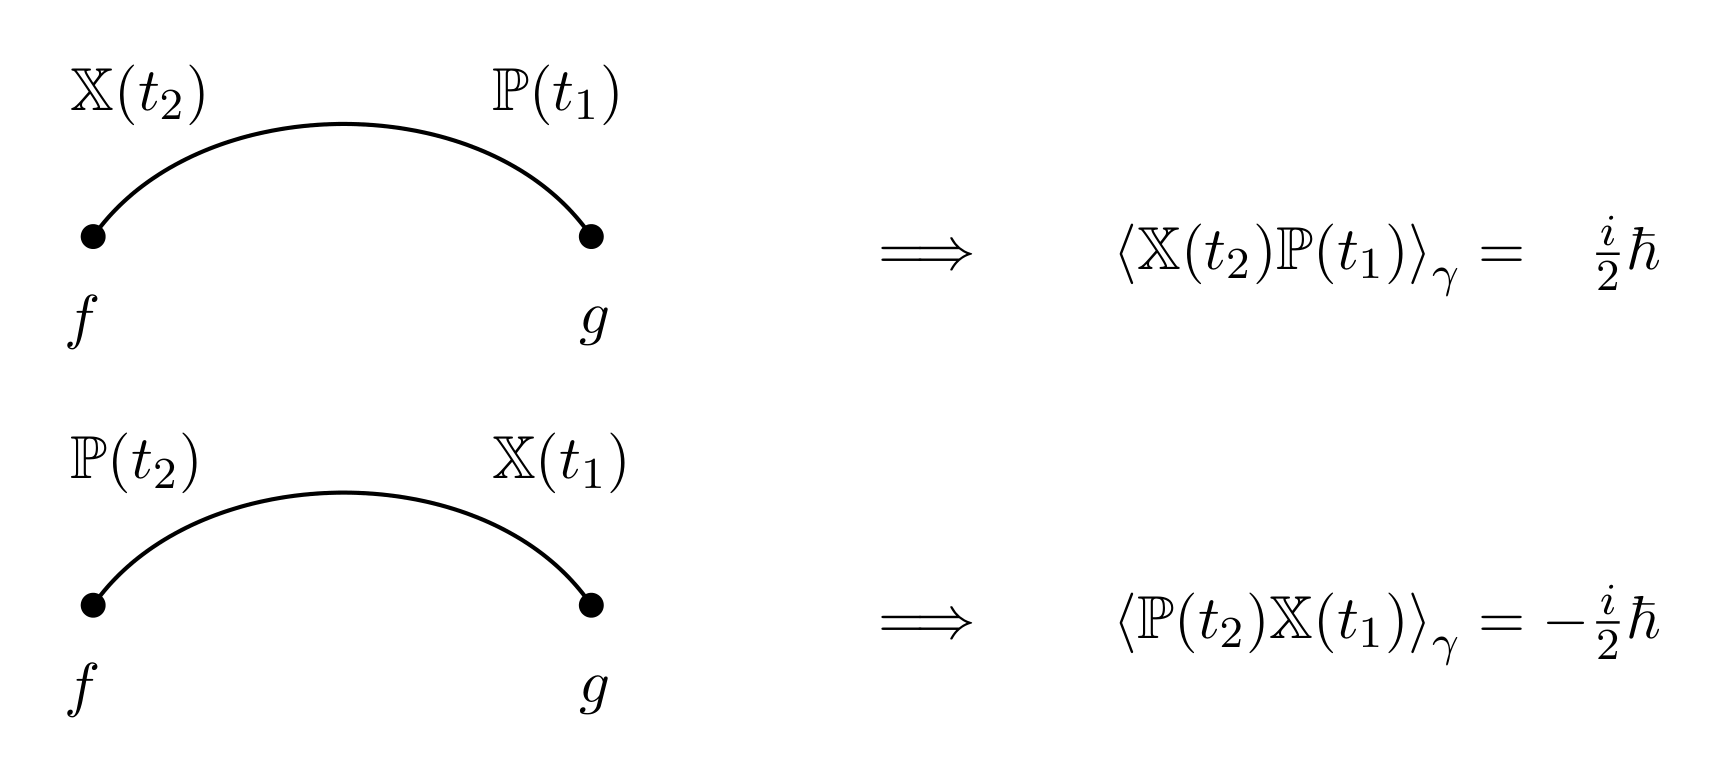
\includegraphics[width=0.69\linewidth]{fig_p044_1.png}
  \caption*{两种收缩及其对应的两点函数（原文 PDF p.44 示意图，原文无编号）}
\end{figure}
\[
  \langle\mathbb{X}(t_2)\mathbb{P}(t_1)\rangle_\gamma=\frac{\ii}{2}\hbar,
  \qquad
  \langle\mathbb{P}(t_2)\mathbb{X}(t_1)\rangle_\gamma=-\frac{\ii}{2}\hbar.
\]
对于有 $m$ 条传播子的图，存在由边置换给出的自同构群 $S_m$，它在 Feynman 图
展开中贡献因子 $\frac{1}{m!}$。于是得到
\[
  \begin{aligned}
    &\langle f(x+\mathbb{X}(t_2),p+\mathbb{P}(t_2))\,
      g(x+\mathbb{X}(t_1),p+\mathbb{P}(t_1))\rangle_\gamma\\
    &\quad=f(x,p)\,\ee^{\frac{\ii}{2}\hbar\left(
        \overleftarrow{\frac{\partial}{\partial x}}
        \overrightarrow{\frac{\partial}{\partial p}}
        -\overleftarrow{\frac{\partial}{\partial p}}
        \overrightarrow{\frac{\partial}{\partial x}}
      \right)}g(x,p)
      =\left(f*_{\hbar}g\right)(x,p),
  \end{aligned}
\]
这恰好就是 Moyal 积。

% [Tutor Note: 自同构因子 $\frac{1}{m!}$ 是 Feynman 图展开中最常见的出错点之一：
% 交换 $m$ 条传播子不改变图，故要除以 $m!$；Moyal 积指数展开的 $m$ 阶项
% $\frac{1}{m!}\left(\frac{\ii\hbar}{2}\right)^m(\cdots)^m$ 正是这一因子的来源。
% 漏掉 $m!$ 会使结果变成 $\ee^{\cdots}$ 而非其泰勒展开。]

我们可以把
\begin{figure}[htbp]
  \centering
  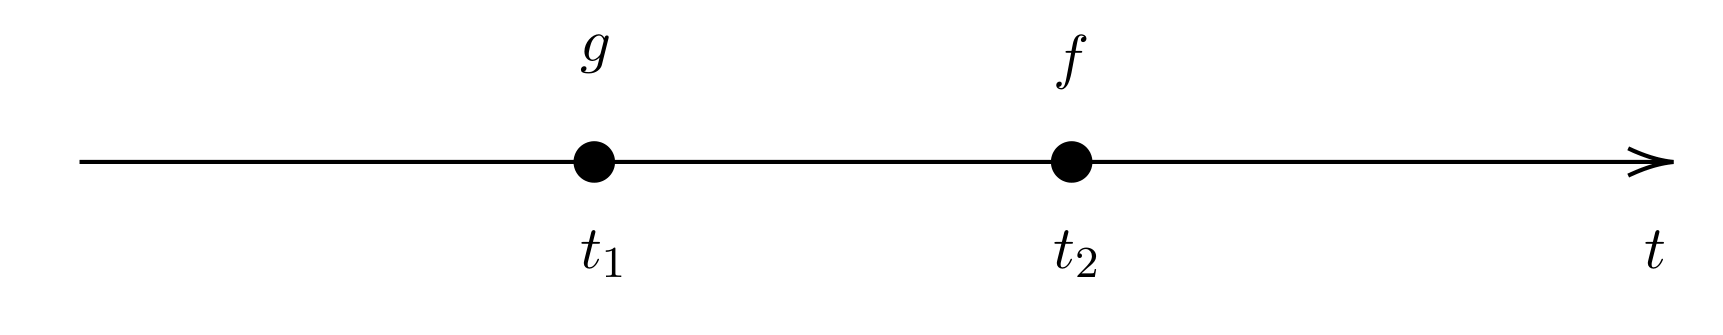
\includegraphics[width=0.69\linewidth]{fig_p044_2.png}
  \caption*{在时间轴上依次插入 $g$ 与 $f$（原文 PDF p.44 示意图，原文无编号）}
\end{figure}
看作在时刻 $t_1$ 插入一个算子 $g$，然后在较晚的时刻 $t_2$ 插入另一个算子 $f$。
总的效果是两个算子的复合，它在量子力学中由 Moyal 积 $f*_{\hbar}g$ 表示。

这一图像也给出 Moyal 积 $*_{\hbar}$ 结合性的简单解释。给定三个函数
$f,g,h$，按时间顺序插入它们
\begin{figure}[htbp]
  \centering
  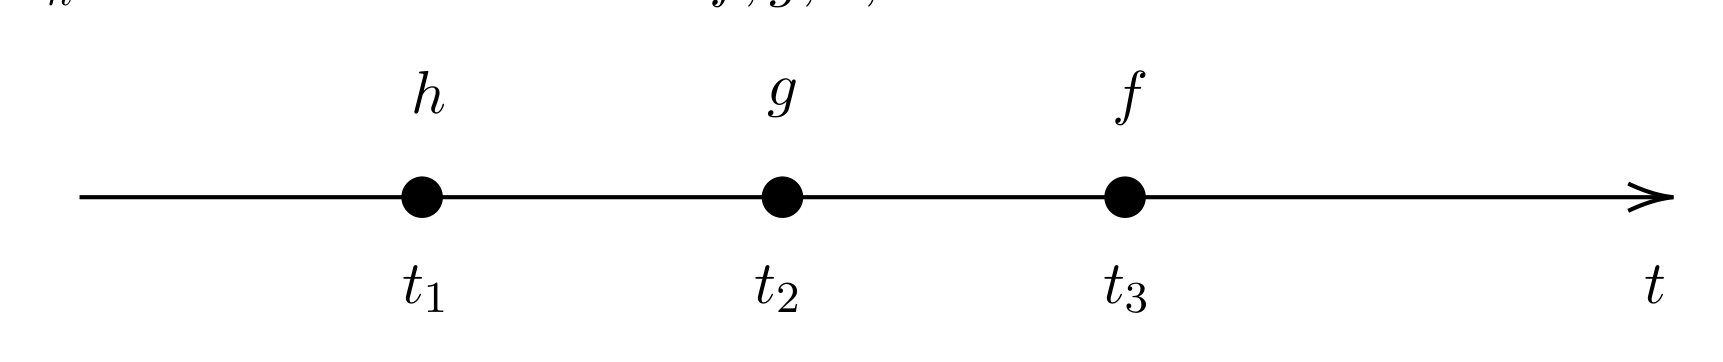
\includegraphics[width=0.69\linewidth]{fig_p044_3.png}
  \caption*{在时间轴上依次插入 $h$、$g$、$f$（原文 PDF p.44 示意图，原文无编号）}
\end{figure}
考虑关联
\[
  \langle f(x+\mathbb{X}(t_3),p+\mathbb{P}(t_3))\,
    g(x+\mathbb{X}(t_2),p+\mathbb{P}(t_2))\,
    h(x+\mathbb{X}(t_1),p+\mathbb{P}(t_1))\rangle_\gamma.
\]
该值在时间位置的局部形变下不变，只有次序是重要的。由先前的计算
{\small
\[
  \begin{aligned}
    \left(f*_{\hbar}g\right)*_{\hbar}h
    &=\lim_{t_1\to t_2^-}\lim_{t_3\to t_2^+}
      \langle f(x+\mathbb{X}(t_3),p+\mathbb{P}(t_3))\,
      g(x+\mathbb{X}(t_2),p+\mathbb{P}(t_2))\,
      h(x+\mathbb{X}(t_1),p+\mathbb{P}(t_1))\rangle_\gamma,\\
    f*_{\hbar}\left(g*_{\hbar}h\right)
    &=\lim_{t_3\to t_2^+}\lim_{t_1\to t_2^-}
      \langle f(x+\mathbb{X}(t_3),p+\mathbb{P}(t_3))\,
      g(x+\mathbb{X}(t_2),p+\mathbb{P}(t_2))\,
      h(x+\mathbb{X}(t_1),p+\mathbb{P}(t_1))\rangle_\gamma.
  \end{aligned}
\]}
上述关联的拓扑性质蕴含
\[
  \left(f*_{\hbar}g\right)*_{\hbar}h
  =f*_{\hbar}\left(g*_{\hbar}h\right).
\]

% [Tutor Note: 两个极限的次序不可交换：$t_1\to t_2^-$ 从下方逼近、$t_3\to t_2^+$
% 从上方逼近，分别表示“把 $h$ 推到 $g$ 的左侧”“把 $f$ 推到 $g$ 的右侧”。结合性
% 不是来自极限交换，而是来自关联函数对时间位置局部形变的不变性（拓扑性）。
% 原文正是用这一点绕过了“路径积分测度未定义”的困难。]

% >>> p045

\subsection{抵消项与重整化（Counter-term and Renormalization）}

一般而言，由于传播子的奇异性，Feynman 图积分是发散的。为了赋予它们意义并
提取有意义的数值，抵消项（counter-term）方法起着重要作用。我们通过 $\R^4$
上 $\phi^4$ 理论的重整化来说明抵消项的基本思想。作用量为
\[
  S[\phi]=\frac{1}{2}\int_{\R^4}\dd^4x\,\phi D\phi
  +\frac{\lambda}{4!}\int_{\R^4}\dd^4x\,\phi^4,
  \qquad \phi\in C_c^{\infty}(\R^4),
\]
其中
\[
  D=-\sum_{i=1}^{4}\frac{\partial}{\partial x^i}\frac{\partial}{\partial x^i},
\]
$\lambda$ 是耦合常数。传播子 $D^{-1}$ 由 Green 函数给出
\[
  G(x,y)=\frac{1}{|x-y|^2},\qquad x,y\in\R^4.
\]
相互作用项给出一个四价顶点。
\begin{figure}[htbp]
  \centering
  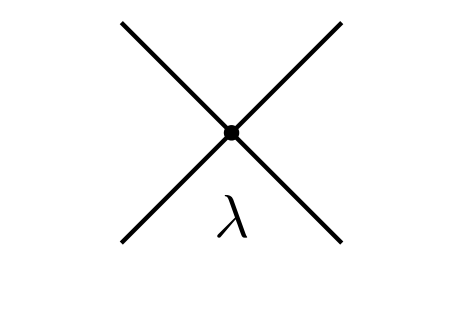
\includegraphics[width=0.22\linewidth]{fig_p045_1.png}
  \caption*{四价顶点（原文 PDF p.45 示意图，原文无编号）}
\end{figure}

% [Tutor Note: 原文的 Laplace 算子取 $D=-\sum_i\partial_i\partial_i$，即通常的
% $-\Delta$，没有 $\frac{1}{2}$ 因子；相应的 Green 函数写成 $G=1/|x-y|^2$
% （在 $\R^4$ 上，$-\Delta$ 的基本解通常是 $\frac{1}{4\pi^2|x-y|^2}$）。
% 因此原文的 $G$ 与常见归一化相差常数 $4\pi^2$。这不是笔误而是作者的归一化
% 约定（把常数吸收进 $D$ 或 $\lambda$ 的定义），但读者自行代入标准公式时极易
% 对不上系数，特此提示。]

\paragraph{树图（Tree diagrams）}

让我们从一个树图出发
\begin{figure}[htbp]
  \centering
  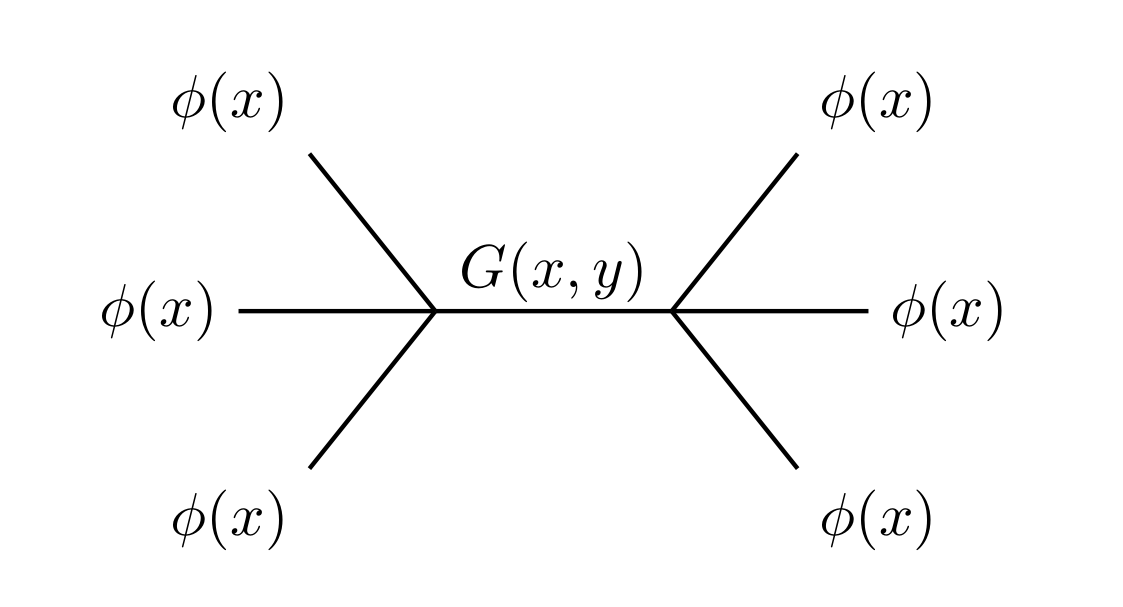
\includegraphics[width=0.45\linewidth]{fig_p045_2.png}
  \caption*{树图（原文 PDF p.45 示意图，原文无编号）}
\end{figure}
\[
  \begin{aligned}
    &=\lambda^2\int_{\R^4\times\R^4}\dd^4x\,\dd^4y\,
      \phi(x)^3\phi(y)^3\,G(x,y)\\
    &=\lambda^2\int_{\R^4\times\R^4}\dd^4x\,\dd^4y\,
      \phi(x)^3\phi(y)^3\,\frac{1}{|x-y|^2}.
  \end{aligned}
\]
对任何紧支集的输入 $\phi$，这是收敛的。事实上，所有树图都收敛。唯一的潜在
发散出现在我们允许 $\phi$ 在无穷远处没有适当衰减时。这称为\emph{IR 发散}
（红外发散），源自时空流形的非紧性；它不如 UV 发散（紫外发散）严重。

% [Tutor Note: “所有树图都收敛”是因为树图的内线传播子 $1/|x-y|^2$ 只在
% $x=y$ 处奇异，不会出现多圈图中的重叠发散；但 $x,y$ 都在非紧的 $\R^4$ 上积分，
% 当 $\phi$ 在无穷远处衰减不够快时积分可能发散，这就是 IR 发散。原文说它
% “不如 UV 发散严重”，因为在紧支集 $\phi$ 下 IR 发散并不出现。]

\paragraph{单圈图（One-loop diagrams）}

考虑一个单圈图
\begin{figure}[htbp]
  \centering
  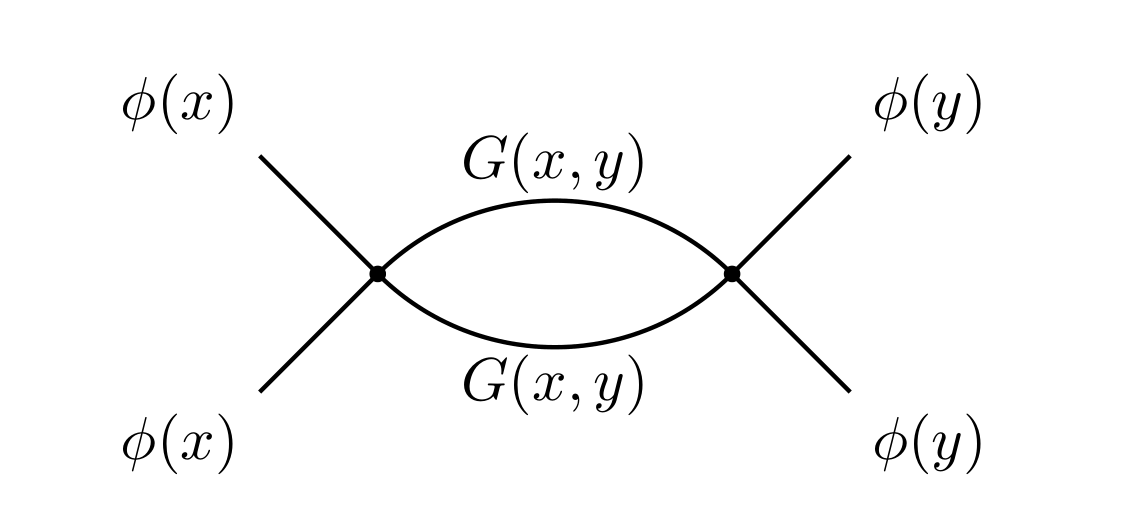
\includegraphics[width=0.45\linewidth]{fig_p045_3.png}
  \caption*{单圈图（原文 PDF p.45 示意图，原文无编号）}
\end{figure}

% >>> p046

于是有
\[
  \begin{aligned}
    &=\hbar\lambda^2\int_{\R^4\times\R^4}\dd^4x\,\dd^4y\,
      \phi(x)^2\phi(y)^2\,G(x,y)^2\\
    &=\hbar\lambda^2\int_{\R^4\times\R^4}\dd^4x\,\dd^4y\,
      \phi(x)^2\phi(y)^2\,\frac{1}{|x-y|^4}.
  \end{aligned}
\]
这通常是在 $x=y$ 附近发散的积分。著名的重整化思想按如下三步策略给出解决方案。
\begin{enumerate}[label=(\arabic*),leftmargin=2.2em,itemsep=0.15em]
  \item 用截断参数 $\eps$ 正则化 $G$；
  \item 要求耦合常数（此处为 $\lambda$）依赖于截断 $\eps$；
  \item 适当选取 (1) 与 (2)，使得去掉截断后计算结果具有有限值。
\end{enumerate}

物理学中常用的正则化是动量截断。设 $k$ 为 $x$ 的 Fourier 变换，则可以用
$|k|$ 的截断 $[\Lambda_0,\Lambda_1]$ 来正则化 Green 函数 $G(x,y)$：
\[
  G(x,y)=\int_{\R^4}\dd^4k\,\frac{\ee^{\ii k(x-y)}}{k^2}
  \quad\leadsto\quad
  \int_{\Lambda_0\le |k|\le\Lambda_1}\dd^4k\,
  \frac{\ee^{\ii k(x-y)}}{k^2}.
\]
动量截断是自然的，也是物理学中最常用的。但它在一般流形上并不方便。我们也可
使用热核截断。对 Laplace 算子 $D$，Green 函数是热核 $\ee^{-tD}$ 的时间积分：
\[
  G(x,y)=\int_0^{\infty}\ee^{-tD}\dd t.
\]
我们选取 UV 截断 $\eps$ 与 IR 截断 $L$。则正则化传播子为
\[
  P_{\eps}^{L}=\int_{\eps}^{L}\ee^{-tD}\dd t
  =\int_{\eps}^{L}\frac{\dd t}{(2\pi t)^2}\,
  \ee^{-\frac{|x-y|^2}{4t}}.
\]

% [Tutor Note: 这里的 heat kernel 归一化疑有笔误：$\R^4$ 上 $-\Delta$ 的热核为
% $(4\pi t)^{-2}\ee^{-|x-y|^2/(4t)}$，原文分母写作 $(2\pi t)^2$（即 $4\pi^2t^2$），
% 与标准结果相差因子 $4^2=16$。这会影响下面 $\log\eps$ 的系数归一化。按体例
% 照录原文并在此提示，请核对原书 p.45 / PDF p.46。]

正则化后的单圈图变为（细节留给读者）
\begin{figure}[htbp]
  \centering
  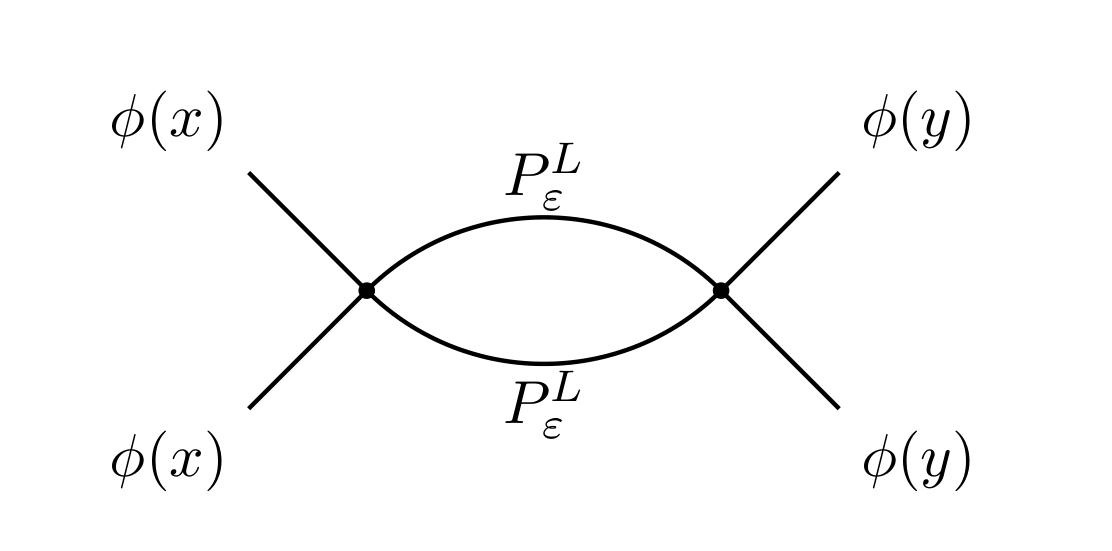
\includegraphics[width=0.45\linewidth]{fig_p046_1.png}
  \caption*{用正则化传播子 $P_\eps^L$ 替换后的单圈图（原文 PDF p.46 示意图，原文无编号）}
\end{figure}
\[
  \begin{aligned}
    &=\hbar\lambda^2\int_{\R^4\times\R^4}\dd^4x\,\dd^4y\,
      \phi(x)^2\phi(y)^2\,P_{\eps}^{L}(x,y)^2\\
    &=\hbar\lambda^2\int_{\R^4\times\R^4}\dd^4x\,\dd^4y\,
      \phi(x)^2\phi(x+y)^2
      \int_{\eps}^{L}\int_{\eps}^{L}
      \frac{\dd t_1}{(2\pi t_1)^2}\frac{\dd t_2}{(2\pi t_2)^2}\,
      \ee^{-\frac{|y|^2}{4}\left(\frac{1}{t_1}+\frac{1}{t_2}\right)}\\
    &=-\hbar\lambda^2\frac{\log\eps}{\pi^2}
      \int_{\R^4}\dd^4x\,\phi(x)^4
      +\text{当 }\eps\to0\text{ 时光滑的项}.
  \end{aligned}
\]
% [Tutor Note: 第二行中被积函数里的 $\phi$ 已从 $\phi(x)^2\phi(y)^2$ 改写为
% $\phi(x)^2\phi(x+y)^2$：这是把 $P_\eps^L(x,y)^2$ 中的相对坐标 $y$ 重命名为
% 积分变量 $y$ 后的结果（平移不变性），两处 $y$ 含义不同，抄写时容易混。]

% >>> p047

于是我们可以通过加上一个抵消项 $I^{CT}(\eps)$ 来修正作用量 $S$：
\[
  S+I^{CT}(\eps)
  =\frac{1}{2}\int_{\R^4}\dd^4x\,\phi D\phi
  +\frac{\lambda}{4!}\int_{\R^4}\dd^4x\,\phi^4
  +\frac{\log\eps}{4!\pi^2}\hbar\lambda^2\int_{\R^4}\dd^4x\,\phi^4.
\]
该抵消项给出一个新的单圈顶点
\begin{figure}[htbp]
  \centering
  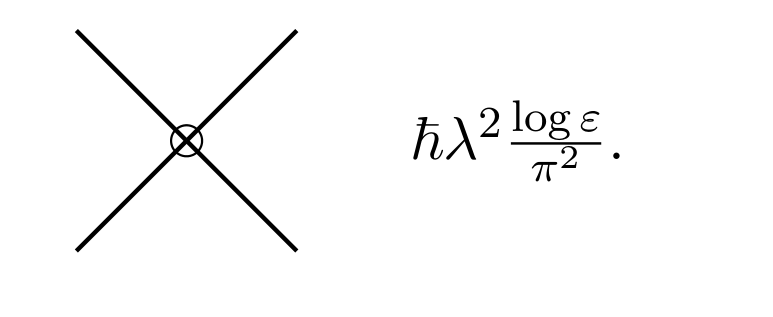
\includegraphics[width=0.31\linewidth]{fig_p047_1.png}
  \caption*{抵消项给出的新顶点（原文 PDF p.47 示意图，原文无编号）}
\end{figure}
\[
  \frac{\hbar\lambda^2\log\eps}{\pi^2}.
\]

% [Tutor Note: $4!$ 的记账是抵消项部分的关键：作用量里的抵消项系数是
% $\frac{\log\eps}{4!\pi^2}\hbar\lambda^2$，但四价顶点带 $4!$ 个外部leg的置换，
% 因此该顶点在图上贡献 $\frac{\hbar\lambda^2\log\eps}{\pi^2}$，恰与单圈结果
% $-\frac{\hbar\lambda^2\log\eps}{\pi^2}\phi(x)^4$ 相消。切勿把作用量系数直接
% 与单圈结果相加；这是初学者最常犯的错误。]

现在若计算带 4 个外线输入的单圈图，我们发现两项贡献
\begin{figure}[htbp]
  \centering
  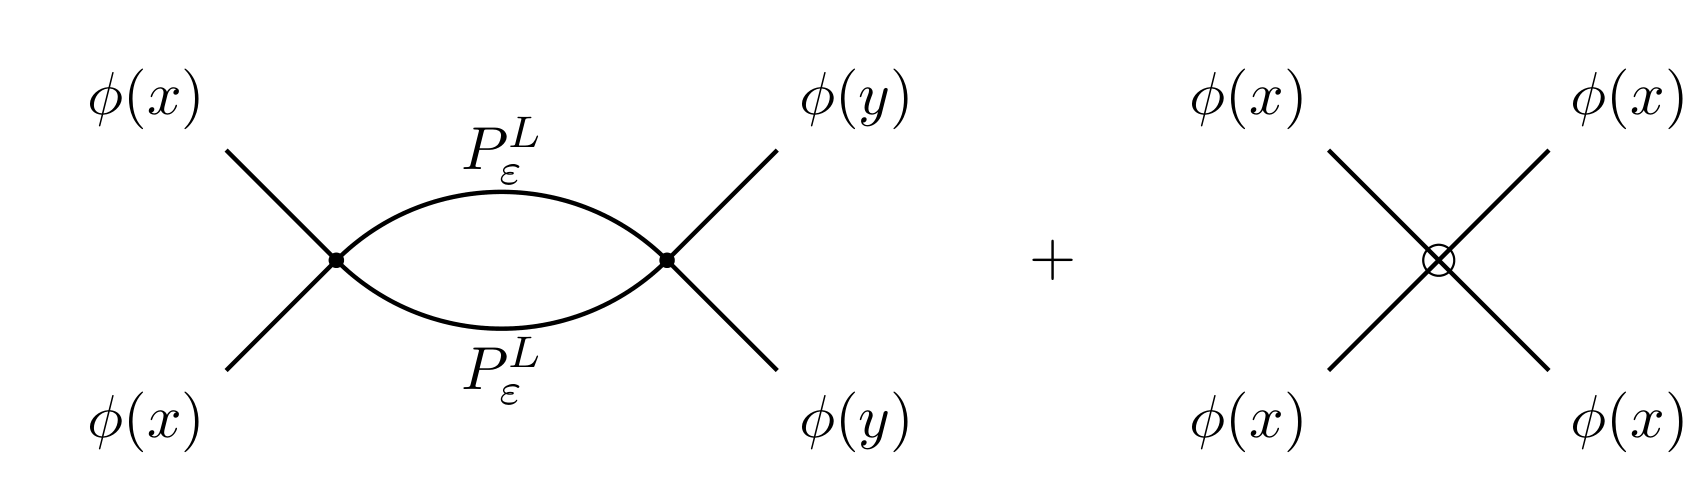
\includegraphics[width=0.68\linewidth]{fig_p047_2.png}
  \caption*{四点单圈图的两项贡献（原文 PDF p.47 示意图，原文无编号）}
\end{figure}
而由构造，这个和对 $\eps\to0$ 的极限存在。

从作用量看，其效果是把耦合常数修正为
\[
  \lambda\longrightarrow\lambda+\hbar\lambda^2\frac{\log\eps}{\pi^2}.
\]
事实上可以证明，通过加入更高 $\hbar$ 阶的、依赖于 $\eps$ 的项
\[
  \lambda\longrightarrow\lambda+\hbar\lambda^2\frac{\log\eps}{\pi^2}
  +\hbar^2(-)+\cdots,
\]
所有 Feynman 图的 UV 发散会相互抵消！这是可重整化理论的一个例子。

% [Tutor Note: 原文 p.46 写“it can shown that”，应为“it can be shown that”；
% p.46 的“possibley”应为“possibly”，p.45 的“A popular regularization in physics
% in the momentum cut-off”应为“is the momentum cut-off”。以上均为原文笔误，
% 译文按原意处理，不在此改写英文原文。]
一般而言，我们需要在抵消项 $I^{CT}(\eps)$ 中加入许多新项，以抵消所有圈阶的
所有 UV 发散，甚至可能需要无穷多种不同类型的拉格朗日量。如果我们只需要有限项，如
\[
  I^{CT}(\eps)=\lambda_1(\eps)\int\mathscr{L}_1
  +\lambda_2(\eps)\int\mathscr{L}_2
  +\cdots+\lambda_N(\eps)\int\mathscr{L}_N,
\]
并调整有限个系数 $\lambda_1(\eps),\dots,\lambda_N(\eps)$ 以抵消所有发散，则该理论
在物理学中称为“\emph{可重整化的}（renormalizable）”。注意抵消项并不唯一。
引入可重整性这一概念的理由是：我们可以通过有限次实验测量未知的耦合常数，然后
用该理论作出可进一步检验的新预言。如果我们有无穷多个耦合常数，那么理论就没有
预言能力，尽管它在数学上仍然有意义。上述 $\R^4$ 上 $\phi^4$ 理论的例子是可
重整化的。
% [Tutor Note: 本节只讲了 $\phi^4$ 理论单圈抵消项的“操作示范”，并未证明所有圈
% 都可重整；原文的“it can shown”之后直接跳到结论。真正的证明需要 Weinberg
% 幂次计数定理与 BPHZ 减除方案，本讲义在第 7 章用 BV/同伦重整化语言重述，
% 建议读者对照第 7 章阅读。]


% ---------- part07.tex ----------
% ============================================================
%  part07.tex  |  原文 PDF p.48–55（页脚 p.47–54）
%  内容：第 6 章 BRST–BV 形式（BRST-BV Formalism）
%        6.1 商与鬼场（Quotient and Ghost）
%        6.2 多向量场（Polyvector Fields）
%        6.3 Batalin–Vilkovisky（BV）代数
%        6.4 经典 BV 主方程（Classical BV Master Equation，起于 PDF p54）
%  说明：6.5 量子主方程起于 PDF p56，属 part08；本片段止于 p55。
% ============================================================

% >>> p048

\section{BRST--BV 形式（BRST-BV Formalism）}

\begin{keypoints}
  \item \textbf{核心物理图像}：规范理论的轨道空间 $V/G$ 往往奇异，直接在 $V/G$ 上
        积分一般不可行。两条路线是：Faddeev--Popov 型（在 $V$ 上取规范切片 $Y$，
        并以 $\delta(Y)\xi_Y$ 配重使积分在 $Y$ 的连续形变下不变）与 BRST--BV 型
        （用导出商 $V\times\Lie{g}[-1]$ 代替 $V/G$，鬼场正是导出方向的坐标）。
  \item \textbf{数学工具}：Chevalley--Eilenberg 复形
        $C^{\bullet}(\Lie{g},\mathcal{O}(V))$（BRST 微分 $d_{\mathrm{CE}}$）、
        多向量场 $\mathrm{PV}(M)$（即 $\Gamma(M,\wedge^{\bullet}TM)$）、由体积形式诱导的
        BV 算子 $\Delta$（广义散度 / 奇 Laplacian），以及 BV 括号
        （Schouten--Nijenhuis 括号的奇类比）。
  \item \textbf{主要结论}：在 BV 代数 $(A,\Delta)$ 中，
        $\{a,b\}:=\Delta(ab)-(\Delta a)b-(-1)^{|a|}a\Delta b$ 度量 $\Delta$ 偏离
        导子的程度；若 $S_0$ 满足经典主方程 $\{S_0,S_0\}=0$，则
        $\delta=\{S_0,-\}$ 满足 $\delta^2=0$，给出经典 BRST 微分；任何 $G$-不变
        经典作用量都可自然延拓为 CME 的解（BV 形式的普适性）。
  \item \textbf{译者评注}：本章是全书技术核心之一，难点集中在\emph{奇偶符号}、
        $\Delta$ 的归一化与 Schouten 括号的符号约定；6.4 节只给出经典主方程，
        量子主方程（QME）与相关上同调的解释留待第 6.5 节（part08）。
\end{keypoints}

我们讨论经典与量子规范理论的 BRST--BV 形式。本节我们聚焦于有限维玩具模型，
以说明主要结构。下一节我们讨论如何纳入重整化。

\subsection{商与鬼场（Quotient and Ghost）}

考虑如下有限维规范理论玩具模型
\[
  f:\ V\longrightarrow\C,
\]
其中连通 Lie 群 $G$ 作用在 $V$ 上，且 $f$ 是 $G$-不变的。等价地，$f$ 是 $V/G$
上的函数，而我们关心轨道空间上的积分
\[
  \int_{V/G}\ee^{\frac{1}{\hbar}f}(-).
\]
通常有两种处理方式。

\textcircled{1}\ 寻找一个子空间 $Y\subset V$，使得 $Y$ 中的点代表 $G$ 的轨道，
并构造一个与 $Y$ 相联系的“形式” $\xi_Y$，使得
\[
  \int_V \ee^{\ii f/\hbar}\delta(Y)\xi_Y(-)
\]
在 $Y$ 的连续形变下保持不变。这里的 $Y$ 称为\emph{规范固定条件}。著名的
Faddeev--Popov 方法即属此类。
\begin{figure}[htbp]
  \centering
  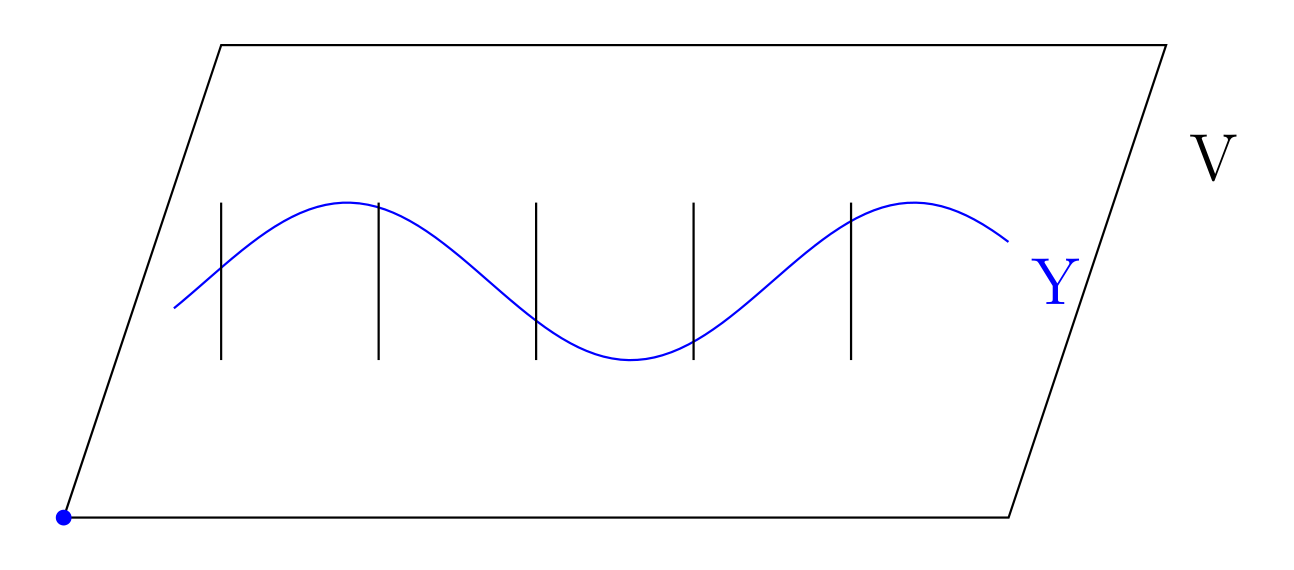
\includegraphics[width=0.52\linewidth]{fig_p048_1.png}
  \caption*{规范固定切片：$Y\subset V$（原文 Figure 2，原文 p.47 / PDF p.48）}
\end{figure}

% [Tutor Note: 两种方案的几何区别要抓住：Faddeev–Popov 仍在原空间 $V$ 上积分，
% 只是插入 $\delta(Y)\xi_Y$ 把积分“压”到切片 $Y$ 上，并证明结果不随 $Y$ 的连续
% 形变而变（这相当于在 $V$ 上构造了一个闭形式）；BRST–BV 则改用导出商
% $V\times\Lie{g}[-1]$，从而在轨道空间 $V/G$ 本身有奇点时仍然有效。原文
% $\delta(Y)\xi_Y$ 里的 $\xi_Y$ 是与 $Y$ 的选取相关的伴随“形式”，作者未写出其
% 具体表达式，此处不宜擅自补全。]

当商 $V/G$ 的奇异性不强时，上述构造效果很好。一般地，若轨道空间 $V/G$ 是
“坏”的，就会出现新问题。这是几何中的典型问题，而教训是我们应当取导出对象
来消解奇异性。这引出了另一种方法。

\textcircled{2}\ BRST--BV 方法。令 $\mathcal{O}(V)$ 表示 $V$ 上的函数。则 $V/G$
上的函数
\[
  \mathcal{O}(V/G)=\mathcal{O}(V)^G
\]
可以自然地等同于 $V$ 上的 $G$-不变函数。假设 $G$ 是连通 Lie 群，Lie 代数为
$\Lie{g}$。每个 $u\in\Lie{g}$ 生成 $V$ 上的一个向量场 $X_u$，而 $G$-不变函数
可以无穷小地表示为
\[
  \mathcal{O}(V)^G=\{\phi\in\mathcal{O}(V)\mid X_u(\phi)=0,\ \forall u\in\Lie{g}\}.
\]

% >>> p049

设 $\{e_1,\dots,e_m\}$ 为 $\Lie{g}$ 的一组基，
$\{c^1,\dots,c^m\}$ 为 $\Lie{g}^{\vee}$ 的对偶基。记 $X_\alpha:=X_{e_\alpha}$。
回顾 Chevalley--Eilenberg 微分（BRST）
\[
  \begin{aligned}
    d_{\mathrm{CE}}:\ \mathcal{O}(V)&\longrightarrow
      \Lie{g}^{\vee}\otimes\mathcal{O}(V),\\
    \phi&\longmapsto\sum_\alpha c^\alpha\otimes X_\alpha(\phi).
  \end{aligned}
\]
我们有如下自然的正合列
\[
  0\longrightarrow\mathcal{O}(V)^G\longrightarrow\mathcal{O}(V)
  \longrightarrow\Lie{g}^{\vee}\otimes\mathcal{O}(V).
\]
现在清楚了：完整的 Chevalley--Eilenberg 复形
\[
  C^{\bullet}(\Lie{g},\mathcal{O}(V))
  =\left(\wedge^{\bullet}\Lie{g}^{\vee}\otimes\mathcal{O}(V),
  d_{\mathrm{CE}}\right)
\]
是 $\mathcal{O}(V)^G$ 的一个自然的导出替代（derived replacement）。
$\Lie{g}^{\vee}$ 中的反交换变量 $c^i$ 称为\emph{鬼场}，如此前所见。由于
\[
  \wedge^{\bullet}\Lie{g}^{\vee}
  =\Sym^{\bullet}\left(\Lie{g}^{\vee}[-1]\right)
  =\Sym^{\bullet}\left((\Lie{g}[1])^{\vee}\right),
\]
我们可以把 $\wedge^{\bullet}\Lie{g}^{\vee}$ 看作（奇）分次空间 $\Lie{g}[-1]$
上的自由多项式环。于是
\[
  C^{\bullet}(\Lie{g},\mathcal{O}(V))=
  V\times\Lie{g}[-1]\ \text{上的函数}.
\]
这是一个 dg 空间，因为 $C^{\bullet}(\Lie{g},\mathcal{O}(V))$ 是以
Chevalley--Eilenberg 微分为微分的 dg 代数
\[
  d_{\mathrm{CE}}
  =\frac{1}{2}f^{\gamma}_{\ \alpha\beta}c^{\alpha}c^{\beta}
  \frac{\partial}{\partial c^{\gamma}}+c^{\alpha}X_{\alpha}.
\]
我们应把 $V\times\Lie{g}[-1]$ 看作 $V$ 的导出 $G$-商。我们的下一个目标是在
$V\times\Lie{g}[-1]$ 上建立积分理论
\[
  \int_{V\times\Lie{g}[1]}\ee^{f/\hbar},
\]
使其能够自然推广到 QFT 的 $\infty$ 维情形。

% [Tutor Note: 上面这个正合列只在 $H^0$ 处给出不变函数：连通 $G$ 时
% $H^0(\Lie{g}^{\vee}\otimes\mathcal{O}(V))=\mathcal{O}(V)^G$，但右端映射一般不是
% 满射，$H^1$ 度量的是“不能由单个无穷小对称生成的规范冗余”。原文称其为
% “natural exact sequence” 是简写，严格地说应读作上链复形的正合列的一部分。]

% [Tutor Note: 这里两次出现 $\Lie{g}[-1]$，最后一行积分却写成
% $\int_{V\times\Lie{g}[1]}$，前后记号不一致，疑为原文笔误（应为
% $V\times\Lie{g}[-1]$：鬼场 $c^\alpha$ 的次数为 $+1$，作为坐标它属于
% $\Lie{g}[-1]$）。按体例照录原文，请核对原书 p.48 / PDF p.49。]

% [Tutor Note: $d_{\mathrm{CE}}=\frac{1}{2}f^{\gamma}_{\ \alpha\beta}
% c^{\alpha}c^{\beta}\partial_{c^{\gamma}}+c^{\alpha}X_{\alpha}$ 中的 $\frac{1}{2}$
% 依赖结构常数对 $(\alpha,\beta)$ 反对称 $f^{\gamma}_{\ \alpha\beta}
% =-f^{\gamma}_{\ \beta\alpha}$。若某文献的结构常数用不同的对称化约定，这个
% $\frac{1}{2}$ 与整体符号都要相应调整；这是核对 BRST 公式时最常见的差异来源。]

\subsection{多向量场（Polyvector Fields）}

现在我们讨论关于积分的另一种观点。设 $M$ 是 $n$ 维定向流形（或简单地取
$\R^n$）。设 $\Omega$ 是 $M$ 上的体积形式。它定义了
\[
  \begin{aligned}
    \int:\ C^{\infty}(M)&\longrightarrow\R,\\
    f&\longmapsto\int_M\Omega f.
  \end{aligned}
\]
几何上，体积形式 $\Omega$ 诱导出散度算子
\[
  \operatorname{Div}:\ \operatorname{Vect}(M)\longrightarrow C^{\infty}(M),
\]
其定义为
\[
  \int\Omega\operatorname{Div}(X)\rho
  =-\int\Omega X(\rho),\qquad \forall\rho\in C_c^{\infty}(M).
\]
具体地，
\[
  \operatorname{Div}(X)=\frac{\mathcal{L}_X\Omega}{\Omega}
  =\frac{\dd\iota_X\Omega}{\Omega}.
\]

% [Tutor Note: 这里散度的符号约定是全局性的：$\int\Omega\,\mathrm{Div}(X)\rho
% =-\int\Omega\,X(\rho)$ 中的负号来自分部积分（无边界项，因 $\rho$ 紧支集），
% 它决定了 $\mathrm{Div}=\Delta|_{\mathrm{PV}^1}$ 的符号，进而决定整个 BV 算子
% $\Delta$ 的符号。若把 $\Delta$ 与 $\mathrm{Div}$ 差一个负号，后面的 CME/QME
% 都会跟着变号；核对时务必先固定这一约定。]

% >>> p050

\begin{wdefn}{6.1}
我们定义\emph{多向量场}
\[
  \mathrm{PV}(M)=\bigoplus_k \mathrm{PV}^k(M),
  \qquad\text{其中}\qquad
  \mathrm{PV}^k(M):=\Gamma(M,\wedge^k TM),\quad k\ge 0.
\]
对 $\alpha\in\mathrm{PV}^k(M)$，记 $|\alpha|=k$。
\end{wdefn}

注意微分形式是
\[
  \Omega^k(M)=\Gamma(M,\wedge^k T^{\vee}_M).
\]
因此多向量场可以看作微分形式的对偶概念。$\mathrm{PV}(M)$ 带有类似的外积
代数结构
\[
  \mathrm{PV}^k(M)\otimes\mathrm{PV}^l(M)
  \xrightarrow{\ \wedge\ }\mathrm{PV}^{k+l}(M),
\]
它是分次交换的
\[
  \alpha\wedge\beta=(-1)^{|\alpha||\beta|}\beta\wedge\alpha.
\]
当 $k=1$ 时，$\mathrm{PV}^1(M)=\operatorname{Vect}(M)$ 正是向量场。

体积形式 $\Omega$ 让我们可以用下式把多向量场与微分形式等同起来
\[
  \begin{aligned}
    \Gamma:\ \mathrm{PV}^k(M)&\xrightarrow{\ \Omega\ }\Omega^{n-k}(M),\\
    \mu&\longmapsto\mu\lrcorner\,\Omega.
  \end{aligned}
\]
这里对 $\mu=X_1\wedge X_2\wedge\cdots\wedge X_k$，$X_i\in\operatorname{Vect}(M)$，
\[
  \mu\lrcorner\,\Omega=\iota_{X_1}\iota_{X_2}\cdots\iota_{X_k}\Omega.
\]
由于 $\Omega$ 是体积形式，$\Gamma$ 给出线性同构
$\mathrm{PV}^k\overset{\simeq}{\longrightarrow}\Omega^{n-k}$。

我们可以用 $\Gamma$ 把 de Rham 复形 $(\Omega^{\bullet}(M),\dd)$ 变换到
$\mathrm{PV}(M)$ 上：
\begin{figure}[htbp]
  \centering
  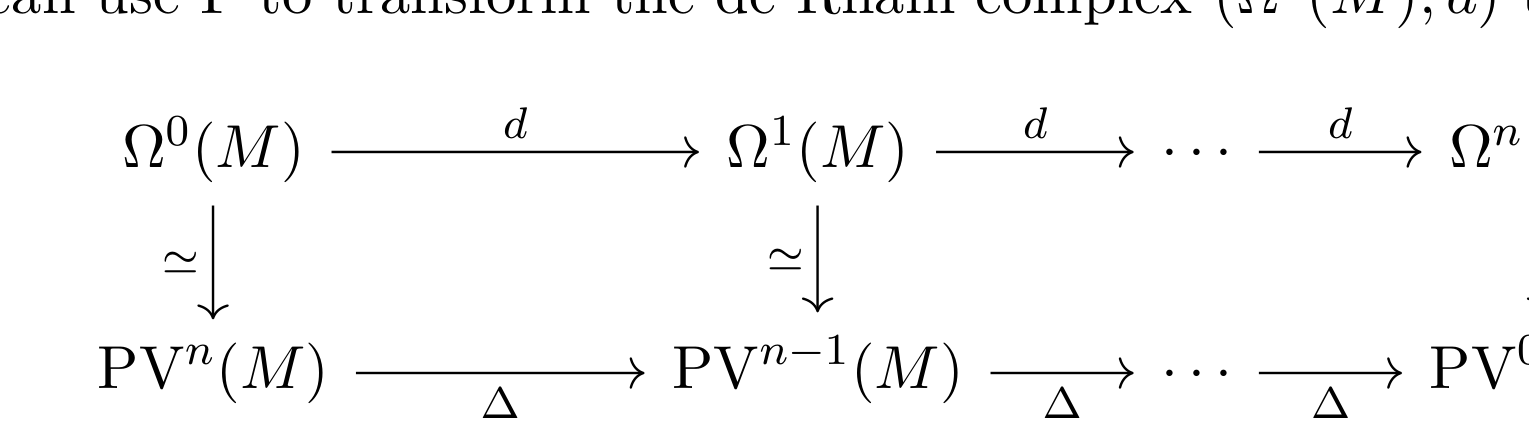
\includegraphics[width=0.61\linewidth]{fig_p050_1.png}
  \caption*{de Rham 复形与多向量场复形之间的同构（原文 PDF p.50 示意图，原文无编号）}
\end{figure}
验证：$\Delta:\mathrm{PV}^1(M)=\operatorname{Vect}(M)\to\mathrm{PV}^0(M)
=C^{\infty}(M)$ 正是与 $\Omega$ 相联系的散度算子。一般地，
\[
  \Delta:\ \mathrm{PV}^k(M)\longrightarrow\mathrm{PV}^{k-1}(M)
\]
可以看作多向量场上的广义散度算子。注意 $\dd^2=0$ 蕴含
\[
  \Delta^2=0.
\]
在物理学中，$\Delta$ 称为 \emph{Batalin--Vilkovisky（BV）算子}。

为看出 $\Delta$ 的模样，我们在 $U$ 上局部地工作，并选取局部坐标
$\{x^1,\dots,x^n\}$。设
\[
  \Omega=\ee^{\rho(x)}\dd x^1\wedge\cdots\wedge\dd x^n.
\]
局部地，
\[
  \mathrm{PV}(U)=C^{\infty}(U)[\partial_1,\dots,\partial_n],
\]
其中 $\partial_i$ 之间反交换：$\partial_i\wedge\partial_j=-\partial_j\wedge\partial_i$。

% [Tutor Note: 读上方的交换图时请注意两排箭头方向\emph{相反}：上排 de Rham
% 微分的次数是 $+1$，下排 $\Delta$ 的次数是 $-1$（把 $k$ 形式的多向量场送到
% $k-1$ 形式）。这是“多向量场是形式的对偶”这一事实的体现；若把 $\Delta$
% 的次数误记为 $+1$，BV 括号的次数（也是 $+1$）就会算错。]

% >>> p051

为方便起见，引入 Grassmann 变量 $\theta_i$ 来表示
\[
  \theta_i\equiv\partial_j,\qquad \theta_i\theta_j=-\theta_j\theta_i.
\]
于是 $\mu\in\mathrm{PV}(U)$ 可以写成
\[
  \mu=\mu(x^i,\theta_i)=\sum_I\mu_I(x^i)\theta^I.
\]
设 $\frac{\partial}{\partial\theta_i}$ 为关于 $\theta_i$ 的导数，其定义为
\[
  \frac{\partial g}{\partial\theta_i}=0,\qquad
  \frac{\partial(\theta_i g)}{\partial\theta_i}=g,
\]
这里 $g$ 不含 $\theta_i$。这些算子也是反交换的：
\[
  \frac{\partial}{\partial\theta_i}\frac{\partial}{\partial\theta_j}
  =-\frac{\partial}{\partial\theta_j}\frac{\partial}{\partial\theta_i}.
\]
例如
\[
  \begin{aligned}
    \frac{\partial}{\partial\theta_1}\frac{\partial}{\partial\theta_2}
      (\theta_1\theta_2)
    &=-\frac{\partial}{\partial\theta_1}\frac{\partial}{\partial\theta_2}
      (\theta_2\theta_1)
     =-\frac{\partial\theta_1}{\partial\theta_1}=-1,\\
    \frac{\partial}{\partial\theta_2}\frac{\partial}{\partial\theta_1}
      (\theta_1\theta_2)&=1.
  \end{aligned}
\]

% [Tutor Note: 上式第一行左端 $\theta_i\equiv\partial_j$ 的指标不匹配：按定义
% $\theta_i$ 应对偶于 $\partial_i$，即应为 $\theta_i\equiv\partial_i$。原文
% PDF p.51 作 $\theta_i\equiv\partial_j$，疑为笔误，此处照录并提示核对原书
% p.50 / PDF p.51。这个指标错位不影响后文（后文只用 $\theta_i$ 作为独立的
% 奇坐标）。]

\begin{wprop}{6.2}
在上述假设与记号下，有
\[
  \Delta=\sum_i\frac{\partial}{\partial x^i}
  \frac{\partial}{\partial\theta_i}
  +\sum_i\partial_i\rho\,\frac{\partial}{\partial\theta_i}.
\]
\end{wprop}

\begin{proof}
习题。
\end{proof}

特别地，对向量场
\[
  X=\sum_i V^i(x)\frac{\partial}{\partial x^i}
  =\sum_i V^i(x)\theta_i,
\]
我们有
\[
  \operatorname{Div}(X)=\Delta X
  =\sum_i\left(\partial_iV^i+\partial_i\rho\,V^i\right).
\]
这恰是散度的公式。

注意第一项 $\sum_i\frac{\partial}{\partial x^i}\frac{\partial}{\partial\theta_i}$
看起来像一个 Laplacian，但它\emph{不是}——$\theta_i$ 是奇变量。尽管如此，
$\Delta$ 有时被称为 \emph{BV Laplacian}，或\emph{奇 Laplacian}。

回顾积分在同调层面的观点：
\begin{figure}[htbp]
  \centering
  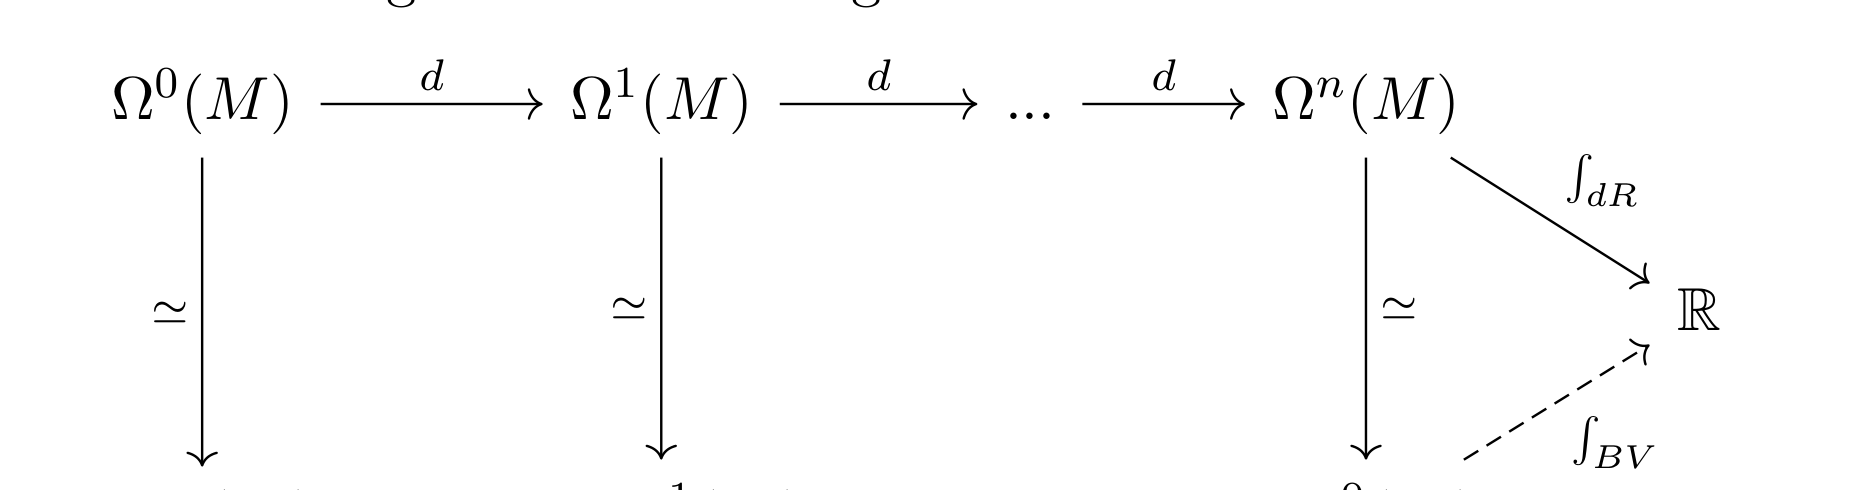
\includegraphics[width=0.75\linewidth]{fig_p051_1.png}
  \caption*{积分的同调观点（原文 PDF p.51 示意图，原文无编号）}
\end{figure}
由该图我们得到
\[
  \int_{dR}\sim H^n_{dR},\qquad \int_{BV}\sim H^0_{\Delta}.
\]
在量子场论中，我们必须处理 $\infty$ 维几何，即 $n=\infty$。此时 $H^n_{dR}$
失去意义，而 $H^0_{\Delta}$ 变得更好，问题便归结为在 QFT 中构造 $\Delta$。
我们将在微扰重整化理论中看到如何做到这一点。

% [Tutor Note: “奇 Laplacian”之名强调 $\Delta$ 是二阶算子且 $\Delta^2=0$，
% 但它的“二阶性”来自奇变量的一阶导数（$\partial_x\partial_\theta$），与通常
% 椭圆 Laplacian 的 ${}^2=0$ 性质完全不同。术语上不要与 Hodge Laplacian
% $\dd\dd^*+\dd^*\dd$ 混淆：后者是偶数阶、不平方为零。]


% >>> p052

\subsection{Batalin--Vilkovisky（BV）代数}

\begin{wdefn}{6.3}
\emph{BV 代数}是一对 $(A,\Delta)$，其中
\begin{itemize}[leftmargin=1.4em,itemsep=0.1em]
  \item[\textcircled{1}] $A$ 是分次交换结合代数：
        $a\cdot b=(-1)^{|a||b|}b\cdot a$，$\forall a,b\in A$；
  \item[\textcircled{2}] $\Delta:A\to A$ 是一个 $\deg=1$ 的“二阶”算子，且
        满足 $\Delta^2=0$。
\end{itemize}
\end{wdefn}

这里“二阶”的意思如下。考虑 $\Delta$ 不是导子的失效程度，用所谓的
\emph{BV 括号}来衡量：
\[
  \{a,b\}:=\Delta(ab)-(\Delta a)b-(-1)^{|a|}a\Delta b.
\]
于是 $\{-,-\}$ 对 $a$ 与 $b$ 两个分量都满足 Leibniz 法则。因此
\[
  \{-,-\}:\ A\times A\longrightarrow A
\]
是 $\deg=1$ 的，并满足

\textcircled{1}\ 分次对称性
\[
  \{a,b\}=(-1)^{|a||b|}\{b,a\}
\]

\textcircled{2}\ 分次 Leibniz 法则
\[
  \{a,bc\}=(-1)^{(1+|a|)|b|}b\{a,c\}+\{a,b\}c
\]

\textcircled{3}\ 由构造，$\{-,-\}$ 与 $\Delta$ 也相容：
\[
  \Delta\{a,b\}=-\{\Delta a,b\}-(-1)^{|a|}\{a,\Delta b\}.
\]
如果我们还有一个
\[
  Q:\ A\longrightarrow A,\qquad \deg=1,
\]
它是导子、平方为零 $Q^2=0$，且与 $\Delta$ 相容
\[
  Q\Delta+\Delta Q=0,
\]
则三元组 $\{A,Q,\Delta\}$ 称为 \emph{DGBV 代数}。

% [Tutor Note: BV 括号定义中的 $(-1)^{|a|}$ 极易放错位置：
% $\{a,b\}=\Delta(ab)-(\Delta a)b-(-1)^{|a|}a\Delta b$。若把它写成
% $(-1)^{|b|}$，分次对称性 $\{a,b\}=(-1)^{|a||b|}\{b,a\}$ 立刻不成立。
% 记忆口诀：第二个“修正项”里的符号要移到 $\Delta$ 越过 $a$ 的位置，故与 $a$
% 的次数有关。]


\begin{wexam}{6.4}
设 $\Omega$ 是 $M$ 上的体积形式，$\Delta$ 是 $\mathrm{PV}(M)$ 上相应的散度
算子。则
\[
  (\mathrm{PV}(M),\Delta)
\]
构成一个 BV 代数。相应的 BV 括号
\[
  \{-,-\}:\ \mathrm{PV}^k(M)\times\mathrm{PV}^l(M)
  \longrightarrow\mathrm{PV}^{k+l-1}(M)
\]
不依赖于 $\Omega$ 的选取，且 $\{-,-\}$ 就是 Schouten--Nijenhuis 括号（至多
差一个符号）（事实上
$\{\alpha,\beta\}=-(-1)^{|\alpha|}\{\alpha,\beta\}_{SN}$）。

在局部坐标下，设
\[
  \Omega=\ee^{\rho(x)}\dd x^1\cdots\dd x^n,
\]
则
\[
  \Delta=\sum_i\frac{\partial}{\partial x^i}
  \frac{\partial}{\partial\theta_i}
  +\sum_i\partial_i\rho\,\frac{\partial}{\partial\theta_i}.
\]
我们得到
\[
  \{x^i,\theta_j\}=\delta^i_{\ j},
  \qquad
  \{x^i,x^j\}=\{\theta_i,\theta_j\}=0.
\]
这是 Poisson 括号的奇类比。
\end{wexam}

% [Tutor Note: Schouten–Nijenhuis 括号在不同文献中的定义相差
% $(-1)^{|\alpha|}$ 或一个整体负号很常见。原文写作
% $\{\alpha,\beta\}=-(-1)^{|\alpha|}\{\alpha,\beta\}_{SN}$，即 BV 括号与 SN 括号
% 差一个与 $|\alpha|$ 有关的符号。按术语表，“Schouten bracket”译作
% “Schouten 括号”，全称“Schouten–Nijenhuis 括号”；原文排印作
% “SchoutenNijenhuis”（缺连字符），属排版笔误。核对符号时请以原书
% p.51 / PDF p.52 为准。]


% >>> p053

\begin{wrem}{6.5}
本例说明了一个关于量子化的重要观点：量子化归结为构造无穷维的体积 / 测度。
\begin{figure}[htbp]
  \centering
  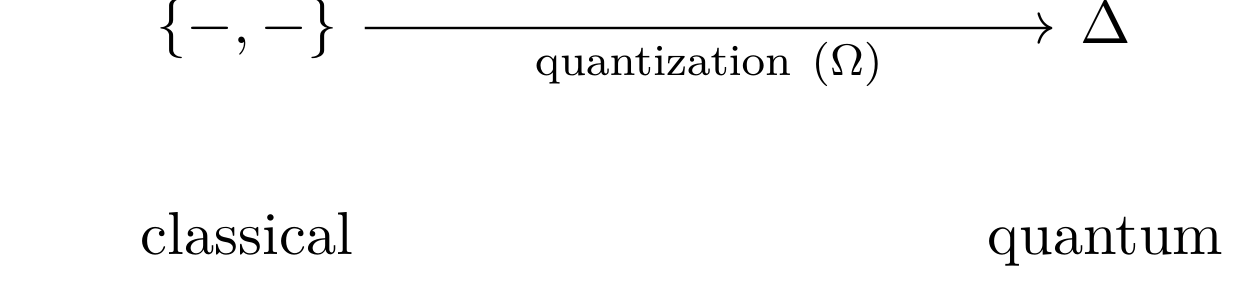
\includegraphics[width=0.50\linewidth]{fig_p053_1.png}
  \caption*{量子化：从经典 Poisson 括号到 BV 算子（原文 PDF p.53 示意图，原文无编号）}
\end{figure}
\end{wrem}

% [Tutor Note: 该图是本章的概念枢纽：把经典一侧的 Poisson 括号 $\{-,-\}$ 换成
% 量子一侧的 BV 算子 $\Delta$（由体积形式 $\Omega$ 构造）。换言之，所谓
% “量子化”就是构造 $\infty$ 维的体积 / 测度，而 $\Delta$ 正是该测度的散度
% 算子。这也是第 7 章有效 BV 量子化与第 9 章 Fedosov 量子化的共同出发点。]

\begin{wexam}{6.6}
设 $X$ 是复流形，$\Omega$ 是全纯体积形式。这样的对 $(X,\Omega)$ 称为
\emph{Calabi--Yau 流形}。我们可以用下式定义多向量场的复类比
\[
  \mathrm{PV}^{k,l}(X)=\Omega^{0,l}\left(X,\wedge^k T^{1,0}_X\right).
\]
设 $\Delta$ 是与 $\Omega$ 相联系的散度算子
\[
  \Delta:\ \mathrm{PV}^{k,l}\longrightarrow\mathrm{PV}^{k-1,l}.
\]
设 $\bar{\partial}$ 是 Dolbeault 微分
\[
  \bar{\partial}:\ \mathrm{PV}^{k,l}\longrightarrow\mathrm{PV}^{k,l+1}.
\]
则 $(\mathrm{PV}^{-\bullet,\bullet},\bar{\partial},\Delta)$ 是一个 DGBV。这里
次数约定是 $\mathrm{PV}^{k,l}$ 的次数为 $l-k$。该 DGBV 控制 $X$ 的形变理论。
\end{wexam}

\begin{wexam}{6.7}
设 $G$ 是 Lie 群，Lie 代数为 $\Lie{g}$。令
\[
  A=\Sym(\Lie{g}^{\vee}[-1])\otimes\Sym(\Lie{g}[2])
  =\C[e_\alpha,c^\alpha].
\]
这里
\begin{itemize}[leftmargin=1.4em,itemsep=0.15em]
  \item $\{e_\alpha\}$ 是 $\Lie{g}$ 的一组基，$\deg(e_\alpha)=-2$。它们彼此
        交换：$e_\alpha e_\beta=e_\beta e_\alpha$。
  \item $\{c^\alpha\}$ 是 $\Lie{g}$ 的对偶基，$\deg(c^\alpha)=1$。它们彼此
        反交换：$c^\alpha c^\beta=-c^\beta c^\alpha$。
  \item $\Delta=\sum_\alpha\frac{\partial}{\partial c^\alpha}
        \frac{\partial}{\partial e_\alpha}$，且
        $\{c^\alpha,e_\beta\}=\delta^\alpha_{\ \beta}$。
\end{itemize}
则 $(A,\Delta)$ 定义一个 BV 代数。

与上面的多向量场构造相比较
\[
  \begin{array}{ccc}
    \deg=1 & c^{\alpha}\longleftrightarrow x^{i} & \deg=0\\[2pt]
    \deg=-2 & e_{\alpha}\longleftrightarrow \theta_{i} & \deg=-1
  \end{array}
\]
我们可以把 $A$ 看作奇空间 $\Lie{g}[1]$ 上的多向量场
\[
  A=\mathrm{PV}(\Lie{g}[1])=\mathcal{O}\left(\Lie{g}[1]\oplus
  \Lie{g}^{\vee}[-2]\right).
\]
\end{wexam}

\begin{wexam}{6.8}
一般地，设 $W$ 是分次向量空间。记
\[
  T^*W[-1]=W\oplus W^{\vee}[-1].
\]
则
\[
  \mathrm{PV}(W):=\mathcal{O}(T^*W[-1])
  =\Sym(W^{\vee})\otimes\Sym(W[1]),
\]
带有典范的 $\deg=1$ 的 BV 括号 $\{-,-\}$。在特殊情形
\begin{itemize}[leftmargin=1.4em,itemsep=0.1em]
  \item $W=\R^n$ $\Longrightarrow$ $\mathrm{PV}(\R^n)$；
  \item $W=\Lie{g}[1]$ $\Longrightarrow$ $\mathrm{PV}(\Lie{g}[1])$。
\end{itemize}
特别地，为了理解 $\int_{V\times\Lie{g}[1]}$，我们将需要考察
\[
  \mathrm{PV}(V\times\Lie{g}[1]).
\]
\end{wexam}

% >>> p054

\subsection{经典 BV 主方程（Classical BV Master Equation）}

现在我们讨论所谓的 \emph{BV 主方程}，它是经典与量子规范理论的基本关系。

\begin{wdefn}{6.9}（经典 BV 主方程）
设 $(A,\Delta)$ 是 BV 代数，$\{-,-\}$ 是 BV 括号。一个次数为 $0$ 的元素
$S_0\in A$ 称为满足\emph{经典 BV 主方程}，若
\[
  \{S_0,S_0\}=0\qquad\text{(CME)}.
\]
\end{wdefn}

$S_0$ 通过
\[
  \delta=\{S_0,-\}:\ A\longrightarrow A
\]
在 $A$ 上诱导一个算子。由于 BV 括号的次数为 $1$、$S_0$ 的次数为 $0$，算子
$\delta$ 的次数为 $1$。并且由 $\{-,-\}$ 的 Leibniz 法则，$\delta$ 是一个导子。

\begin{wprop}{6.10}
CME $\{S_0,S_0\}=0$ 蕴含
\[
  \delta^2=0.
\]
\end{wprop}

\begin{proof}
由 Jacobi 恒等式
\[
  \{\{S_0,S_0\},-\}
  =-2\{S_0,\{S_0,-\}\}
  =-2\delta^2.
\]
\end{proof}


\begin{wexam}{6.11}（对称性）
设 $G$ 是 Lie 群，Lie 代数为 $\Lie{g}$。记 $\{e_\alpha\}$ 为 $\Lie{g}$ 的一组
基，$\{c^\alpha\}$ 为 $\Lie{g}^{\vee}$ 的对偶基。设 $(A,\Delta)$ 是
$\Lie{g}[1]$ 上多向量场的 BV 代数
\[
  A=\Sym(\Lie{g}^{\vee}[-1])\otimes\Sym(\Lie{g}[2])
  =\C[e_\alpha,c^\alpha],\qquad
  \deg(c^\alpha)=1,\quad \deg(e_\alpha)=-2,
\]
且
\[
  \Delta=\sum_\alpha\frac{\partial}{\partial c^\alpha}
  \frac{\partial}{\partial e_\alpha},
  \qquad
  \{c^\alpha,e_\beta\}=\delta^\alpha_{\ \beta}.
\]
在所选基下 Lie 括号为
\[
  [e_\alpha,e_\beta]=\sum_\gamma f^{\gamma}_{\ \alpha\beta}e_\gamma,
\]
其中 $f^{\gamma}_{\ \alpha\beta}$ 是 $\Lie{g}$ 的结构常数。则次数为 $0$ 的
元素
\[
  I=\frac{1}{2}\sum_{\alpha,\beta,\gamma}
  f^{\gamma}_{\ \alpha\beta}c^\alpha c^\beta e_\gamma\in A
\]
满足经典主方程
\[
  \{I,I\}=0.
\]
让我们考虑诱导出的微分
\[
  \delta=\{I,-\}:\ A\longrightarrow A.
\]
\end{wexam}

% [Tutor Note: 本页原文两处笔误：(i) $\deg(e_\alpha=-2)$ 括号错位，应为
% $\deg(e_\alpha)=-2$；(ii) 正文另有一处写作 $\{c^\alpha,e_\alpha\}
% =\delta^\alpha_{\ \beta}$，左端两个指标都是 $\alpha$ 而右端是 $\alpha,\beta$，
% 应为 $\{c^\alpha,e_\beta\}=\delta^\alpha_{\ \beta}$。两处均照录原意并在
% 译文中按正确指标排版，请核对原书 p.53 / PDF p.54。]

% >>> p055

由于 $A=\C[c^\alpha,e_\alpha]$ 是自由代数，我们只需知道 $\delta$ 如何作用在
生成元上。不难看出
\[
  \delta(c^\gamma)=\frac{1}{2}f^{\gamma}_{\ \alpha\beta}c^\alpha c^\beta,
  \qquad
  \delta(e_\alpha)=\frac{1}{2}f^{\gamma}_{\ \alpha\beta}c^\beta e_\gamma.
\]
因此导子 $\delta$ 由向量场
\[
  \delta=\frac{1}{2}\sum_{\alpha,\beta,\gamma}
  f^{\gamma}_{\ \alpha,\beta}c^\alpha c^\beta
  \frac{\partial}{\partial c^\gamma}
  +\sum_{\alpha,\beta,\gamma}
  f^{\gamma}_{\ \alpha\beta}c^\beta e_\gamma
  \frac{\partial}{\partial e_\alpha}
\]
给出。若把 $\delta$ 限制到 $\C[c^\alpha]=\Sym(\Lie{g}^{\vee}[-1])$，则
$\delta=d_{\mathrm{CE}}$。因此
\[
  \left(\Sym(\Lie{g}^{\vee}[-1]),\delta\right)=C^{\bullet}(\Lie{g}).
\]
在完整的 BV 代数 $A$ 上，我们有
\[
  (A,\delta)=C^{\bullet}(\Lie{g},\Sym(\Lie{g}[2])),
\]
其中 $\Lie{g}$ 通过伴随表示作用在 $\Sym(\Lie{g}[2])$ 上。

% [Tutor Note: 本页三处 $\frac{1}{2}$ 的记账需要核对：$\delta(c^\gamma)
% =\frac{1}{2}f^{\gamma}_{\ \alpha\beta}c^\alpha c^\beta$ 与紧随其后的向量场
% 第一项一致；但 $\delta(e_\alpha)$ 被写成
% $\frac{1}{2}f^{\gamma}_{\ \alpha\beta}c^\beta e_\gamma$，而向量场第二项
% $\sum f^{\gamma}_{\ \alpha\beta}c^\beta e_\gamma\partial/\partial e_\alpha$
% 却没有 $\frac{1}{2}$。按 BV 括号直接计算（也可由下方向量场反推），应为
% $\delta(e_\alpha)=f^{\gamma}_{\ \alpha\beta}c^\beta e_\gamma$（无 $\frac{1}{2}$），
% 故第一个式子的 $\frac{1}{2}$ 疑为原文笔误。按体例照录原文，请核对原书
% p.54 / PDF p.55。]

\begin{wexam}{6.12}（对称性 $+$ 物质）
设 $G$ 是作用于流形 $X$ 的 Lie 群，$X$ 的坐标为 $\{x^i\}$，$\{e_\alpha\}$ 是
Lie 代数 $\Lie{g}$ 的一组基。无穷小作用给出一个 Lie 代数同态
\[
  \begin{aligned}
    \Lie{g}&\longrightarrow\operatorname{Vect}(X),\\
    e_\alpha&\longmapsto V_\alpha
    =V^i_\alpha(x)\frac{\partial}{\partial x^i}.
  \end{aligned}
\]
考虑 $G$-不变函数
\[
  f:\ X\longrightarrow\C,
\]
它模拟一个规范不变的经典作用量。考虑
\[
  A=\mathrm{PV}(X\times\Lie{g}[1])=\mathrm{PV}(X)\otimes\mathrm{PV}(\Lie{g}[1])
  =\C[x^i,\theta_i,e_\alpha,c^\alpha],
\]
其中 $\theta_i=\partial_i$，$\{c^\alpha\}$ 是对偶基。我们在下表中总结这些变量。

\begin{center}
\normalfont\small
\begin{tabular}{lcccc}
  \toprule
  变量 & $c^\alpha$ & $x^i$ & $\theta_i$ & $e_\alpha$ \\
  \midrule
  次数（Degree） & $1$ & $0$ & $-1$ & $-2$ \\
  物理意义（Physics） & 鬼场 & （物质）场 & 反场 & 反鬼场 \\
  \bottomrule
\end{tabular}
\end{center}

我们可以把函数 $I=\frac{1}{2}f^{\gamma}_{\ \alpha\beta}c^\alpha c^\beta e_\gamma$
通过纳入 $x$ 与 $G$-不变函数 $f$ 延拓为
\[
  S_0=f(x)+c^\alpha V^i_\alpha(x)\theta_i
  +\frac{1}{2}f^{\gamma}_{\ \alpha\beta}c^\alpha c^\beta e_\gamma.
\]
\end{wexam}

\begin{wprop}{6.13}
$S_0$ 满足经典主方程。
\end{wprop}

\begin{proof}
习题。
\end{proof}

% [Tutor Note: 上表按原文重排（booktabs）。原文表头第一格为空，第一列是
% “Degree / Physics”两行；本译本把变量名提到表头、把“次数”“物理意义”放到
% 第一列，内容与原文一一对应。术语依据：ghost 鬼场、anti-field 反场、
% anti-ghost 反鬼场（术语表）。]

% [Tutor Note: Prop.\ 6.13 的“Proof: Exercise.”省略了实质验证：把
% $S_0=f+c^\alpha V^i_\alpha\theta_i+\frac{1}{2}f^{\gamma}_{\ \alpha\beta}
% c^\alpha c^\beta e_\gamma$ 代入 $\{S_0,S_0\}=0$，需要同时用到
% (i) $f$ 的 $G$-不变性 $V_\alpha(f)=0$；(ii) 结构常数的 Jacobi 恒等式；
% (iii) $\Lie{g}\to\operatorname{Vect}(X)$ 是 Lie 代数同态，即
% $[V_\alpha,V_\beta]=f^{\gamma}_{\ \alpha\beta}V_\gamma$。三者缺一不可，
% 而原文全部省略。]


% ---------- part08.tex ----------
% ============================================================
%  part08.tex  |  原文 PDF p.56–60（页脚 p.55–59）
%  内容：第 6 章（续）
%    6.5 量子 BV 主方程（Quantum BV Master Equation）
%    6.6 形变–障碍理论（Deformation-Obstruction Theory）
%  说明：6.4 节的标题及其 Definition 6.9–Proposition 6.13 位于 PDF p.54–55，
%        归 part07.tex；本片段自 PDF p.56 起，开头一段是 6.4 末尾的过渡文字，
%        随后进入 6.5。故此处不重复 \section 与 keypoints。
% ============================================================

% >>> p056

于是，任何规范不变的作用量（即 $f$）都自然地延拓为经典主方程的一个解（即 $S_0$）。
这就是 BV 形式的普适性。下面来看诱导出的微分
\[
  \delta = \{S_0,-\}.
\]
把 $S_0$ 写成 $S_0 = f + J$，其中
\[
  J = c^\alpha V_\alpha^i(x)\theta_i + \frac{1}{2} f^{\gamma}_{\alpha\beta}\, c^\alpha c^\beta e_\gamma .
\]
对 $J$ 稍加思索即可看出，$\{J,-\}$ 正是
$C^\bullet(\mathfrak{g},\operatorname{PV}(X)\otimes\Sym(\mathfrak{g}[2]))$ 上的
Chevalley--Eilenberg 微分。这里 $\mathfrak{g}$ 通过 Lie 导数作用于
$\operatorname{PV}(X)$，并通过伴随表示作用于 $\Sym(\mathfrak{g}[1])$。于是
\[
  \delta = d_{\mathrm{CE}} + \{f,-\},
\]
其中 $d_{\mathrm{CE}}$ 表示对称性，而
\[
  \{f,-\} = \sum_i \partial_i f \frac{\partial}{\partial \theta_i}
\]
编码了 $f$ 的临界点，即运动方程。

% [Tutor Note: 原文此段（"Thus any gauge invariant action..."）在手稿中是斜体，
% 接 PDF p.55 上 Proposition 6.13 的证明（原文仅写 "Proof: Exercise."），可视作
% 该习题的解答性注记；译文按普通正文排出，内容不作增删。另，原文 "A few moment
% thought on J" 中 "moment" 应为复数 "moments"，属笔误，按原意译出。]

% [Tutor Note: 易错提醒——原文此句前半写 C^•(g, PV(X)⊗Sym(g[2]))，紧接着却说
% g "acts on Sym(g[1]) via adjoint representation"，两处的移位数不一致；由 6.3 节
% （PDF p.53–55）deg(e_α) = -2 可知 Sym(g[2]) 才是与 {e_α} 匹配的记号，故 "g[1]"
% 疑为 "g[2]" 之笔误。译文照录原文，请核对原书 p.55。此外 d_CE 即第 4 章
% （4.1 节）的 Chevalley–Eilenberg 微分，此处它只作用在鬼场变量 c^α 上。]

\subsection{量子 BV 主方程（Quantum BV Master Equation）}

现在转向讨论量子理论。

\begin{wdefn}{6.14}
  设 $(A,\Delta)$ 是一个 BV 代数。一个 0 次元素
  \[
    S = S_0 + \hbar S_1 + \hbar^2 S_2 + \cdots \in A[[\hbar]]
  \]
  称为满足\textbf{量子（BV）主方程}（quantum (BV) master equation, QME），如果
  \[
    \hbar\Delta S + \frac{1}{2}\{S,S\} = 0.
  \]
  这里把 $\hbar$ 视为形式变量。
\end{wdefn}

在经典极限 $\hbar\to 0$ 下，QME 的首个 $\hbar$ 阶成为
\[
  \frac{1}{2}\{S_0,S_0\} = 0,
\]
这恰是经典主方程。

% [Tutor Note: 易错预警——QME 的写法与符号约定强相关。本书取
% ℏΔS + ½{S,S} = 0；另一些文献（以及作者本人的学生笔记）写成
% {S,S} + 2ℏΔS = 0，二者只差整体乘以 2；还有作者把 Δ 定义成散度算子的相反数，
% 于是符号整体翻转。引用他人结果前务必先核对其 Δ 与 {–,–} 的约定，
% 否则 6.6 节障碍类的符号会全部错位。]

\begin{wprop}{6.15}
  量子主方程等价于
  \[
    \Delta\left(\ee^{\frac{1}{\hbar}S}\right) = 0.
  \]
\end{wprop}

\begin{proof}
  这由 $\Delta$ 的“二阶”性质推出；细节留给读者。
\end{proof}

% [Tutor Note: 此处省略的论证实质——BV 算子是二阶算子，满足
% Δ(fg) = Δf·g + (-1)^{|f|}f·Δg + (-1)^{|f|}{f,g}。代入 f = g = e^{S/ℏ} 得
% Δ(e^{S/ℏ}) = e^{S/ℏ}(ℏ^{-1}ΔS + ℏ^{-2}½{S,S})，故在形式幂级数意义下
% “QME ⟺ Δ(e^{S/ℏ}) = 0”。这一步只是把定义式乘以 e^{S/ℏ} 再整理，
% 不涉及任何额外假设，但要注意 e^{S/ℏ} 不是 A[[ℏ]] 中的元素而是形式指数，
% 展开时按 ℏ 的幂次逐项比较。]

这一表达式给出了 QME 作为量子规范一致性条件的精确物理含义。在微积分中，
若 $\omega$ 是闭微分形式 $d\omega = 0$，则积分
\[
  \int_\gamma \omega
\]
% >>> p057
在闭链 $\gamma$ 上取值，并且该值在 $\gamma$ 的连续形变下保持不变。

BV 理论中有类似的现象。若 $\Delta(\ee^{S/\hbar}) = 0$，则有一种 BV 积分的概念
\[
  \int_{\mathcal{L}} \ee^{\frac{S}{\hbar}},
\]
它在 $\mathcal{L}$ 的连续形变下保持不变。这里 $\mathcal{L}$ 是与规范固定条件相关的
超 Lagrangian 子空间。因此，若 $S$ 满足 QME，则
\[
  \int_{\mathcal{L}} \ee^{\frac{S}{\hbar}}
\]
在规范固定条件的连续变化下保持不变。这正是量子规范一致性的精确表述。

% [Tutor Note: 物理图像点拨——这里的类比是：Δ 扮演外微分 d 的角色，
% e^{S/ℏ} 扮演“闭形式”，而超 Lagrangian 子空间 L（对应一个规范固定切片）
% 扮演“闭链”。规范固定条件的连续变化对应 L 的连续形变，Δ(e^{S/ℏ}) = 0
% （即 QME）保证积分不随形变而变。需要注意，BV 积分 ∫_L 只是一个形式记号
% （见第 7 章借助 (-1)-平移辛结构才把它严格化），不要把它与第 1 章尚未定义的
% 路径积分测度混为一谈。]

假设 $S$ 满足 QME。定义量子 BRST 算子
\[
  \delta^\hbar = \hbar\Delta + \{S,-\}.
\]

% [Tutor Note: 记号提醒——量子 BRST 算子记作 δ^ℏ（ℏ 在上标），经典 BRST 算子
% 记作 δ = {S_0,-}。容易与 6.6 节的 δ_S = {S,-} 混淆：δ_S 只是括号算子本身，
% δ^ℏ = ℏΔ + δ_S。另外 δ^ℏ 一般不再是分次导子（Δ 破坏 Leibniz 法则），
% 但它满足 (δ^ℏ)^2 = 0，仍可定义上同调，此点见 Proposition 6.16。]

\begin{wprop}{6.16}
  $\delta^\hbar$ 满足 $(\delta^\hbar)^2 = 0$。
\end{wprop}

\begin{proof}
  记 $\delta_S = \{S,-\}$。利用
  \[
    \Delta\{S,-\} = -\{\Delta S,-\} - \{S,\Delta(-)\},
  \]
  可得
  \[
    \Delta\delta_S + \delta_S\Delta = -\{\Delta S,-\}.
  \]
  于是
  \[
    \begin{aligned}
      (\delta^\hbar)^2 &= (\hbar\Delta)^2 + \hbar(\Delta\delta_S + \delta_S\Delta) + \delta_S^2\\
      &= -\{\hbar\Delta S,-\} - \frac{1}{2}\{\{S,S\},-\}\\
      &= -\left\{\hbar\Delta S + \frac{1}{2}\{S,S\},-\right\} = 0.
    \end{aligned}
  \]
\end{proof}

% [Tutor Note: 符号约定警示——第二行到第三行之间用了 Jacobi 恒等式把 δ_S²
% 化为 ±½{{S,S},-}；这里出现的负号与本书“Δ{S,-} = -{ΔS,-} - {S,Δ(-)}”
% 的约定绑定。若改用相反的 BV 括号符号（或把 Δ 换成 -Δ），整段的符号会
% 一起翻转，但结论 (δ^ℏ)² = 0 不变。核对时请以定义式（QME 与 Δ 的二阶性质）
% 为准，不要只凭记忆套用；这是 BV 形式中最常见的符号陷阱。]

显然 $\lim_{\hbar\to0}\delta^\hbar = \delta = \{S_0,-\}$ 给出经典 BRST 算子。
因此 $\delta^\hbar$ 可视为 $\delta$ 的量子化。微分 $\delta$ 与 $\delta^\hbar$
分别刻画经典与量子的规范变换。

\begin{wdefn}{6.17}
  设 $(A,\Delta)$ 为 BV 代数，并假设 $S = S_0 + \hbar S_1 + \cdots$ 解量子主方程
  （从而 $S_0$ 解经典主方程）。
  \begin{enumerate}[label=\textcircled{\small\arabic*},leftmargin=2.4em,itemsep=0.2em]
    \item 上同调
          \[
            \Obs^c = H^\bullet(A,\{S_0,-\})
          \]
          称为\textbf{经典可观测量}空间。
    \item 上同调
          \[
            \Obs^q = H^\bullet(A[[\hbar]],\hbar\Delta+\{S,-\})
          \]
          称为\textbf{量子可观测量}空间。
  \end{enumerate}
  它们表示模去规范等价后的经典与量子规范不变对象。
\end{wdefn}

% [Tutor Note: 记号提醒——H^• 中的 • 是“分级”占位符，意为对所有次数的上同调
% 取直和；Obs^c 的上标 c 指 classical，Obs^q 的 q 指 quantum，不是指数。
% 物理上，H^0 对应规范不变的可观测量，H^1 对应无穷小形变/障碍（见 6.6 节），
% 更高次上同调则对应高阶规范结构。]

% >>> p058

\begin{wexam}{6.18}（奇点理论 / Landau--Ginzburg B-模型）
  设 $f:\C^n\to\C$ 是一个在原点有孤立临界点的多项式。考虑由多项式全纯多向量场
  构成的 BV 代数 $(A,\Delta)$：
  \[
    A = \C[z^i,\theta_i],\qquad \theta_i\theta_j = -\theta_j\theta_i,\qquad
    \Delta = \sum_i \frac{\partial}{\partial z^i}\frac{\partial}{\partial \theta_i}.
  \]
  则
  \begin{itemize}[leftmargin=1.6em,itemsep=0.25em]
    \item $f = f(z^i)$ 满足 QME，因为 $f$ 不依赖 $\theta_i$：
      \[
        \Delta\left(\ee^{\frac{1}{\hbar}f(z)}\right) = 0.
      \]
    \item 经典可观测量：
      \[
        \Obs^c = H^\bullet(A,\{f,-\}) = \operatorname{Jac}(f)
        = \C[z^i]/(\partial_i f).
      \]
      这里 $\operatorname{Jac}(f)$ 是 Jacobi 环，$(\partial_i f)$ 是由
      $\partial_i f$ 生成的理想。
    \item 量子可观测量：
      \[
        \Obs^q = H^\bullet(A[[\hbar]],\hbar\Delta+\{f,-\})
        \simeq \Omega^n[[\hbar]]/(\hbar\,\dd + \dd f\wedge)\,\Omega^{n-1}[[\hbar]].
      \]
      这称为（形式的）Brieskorn 格（Brieskorn lattice），在奇点理论中起重要作用。
    \item BV 积分模拟振荡积分
      \[
        \int_{\mathcal{L}} \ee^{\frac{1}{\hbar}f}\mathcal{O},
      \]
      其中 $\mathcal{L}$ 是一个 Lefschetz 快速下降链（Lefschetz thimble）。
  \end{itemize}
  Brieskorn 格与振荡积分都与 Hodge 结构深刻相关。事实上，$\hbar$-进滤过恰是
  Hodge 滤过。因此量子场论可以看作 $\infty$ 维 Hodge 理论的一个版本。
\end{wexam}

% [Tutor Note: 术语与记号依据——（i）本例中出现的花体 \mathcal{O}（BV 积分里的
% 被积可观测量，以及 6.6 节中的障碍类 \mathcal{O}_k）与渐近分析的大 O 记号
% O(ℏ^k) 形状相近但含义完全不同，切勿混用；前者应排作 \mathcal{O}。
% （ii）Jac(f) = C[z^i]/(∂_i f) 称为 f 的 Jacobi 环（局部代数），其维数等于
% f 的孤立临界点重数（Milnor 数）。（iii）“Brieskorn lattice” 中 lattice 指
% D-模意义下的格（与 Hodge 滤过相伴的 Gauss–Manin 联络的格子），故译
% “Brieskorn 格”，不译“晶格”。Lefschetz thimble 是 Picard–Lefschetz 理论中
% 从临界点出发的快速下降流形，译“Lefschetz 快速下降链”。原文“the ℏ-adic
% filtration is precisely the Hodge filtration”一句是本书的核心洞见之一。]

\subsection{形变–障碍理论（Deformation-Obstruction Theory）}

现在我们来回答如下自然的问题：从经典主方程的一个解 $S_0$ 出发，是否总能把它
量子化为量子主方程的解 $S = S_0 + O(\hbar)$？

一般而言，答案是\textbf{否}。可观测量复形恰好控制这一形变理论，并捕捉其中的障碍。

设 $(A,\Delta)$ 为 BV 代数。假设 $S_0$ 解经典主方程，且 $\delta = \{S_0,-\}$。
我们要找 $S_1,S_2,\cdots\in A$，使得
\[
  S = S_0 + S_1\hbar + S_2\hbar^2 + \cdots
\]
解量子主方程。我们按 $\hbar$ 的阶逐阶分析。

% [Tutor Note: 这一段是本节的总纲：把“量子化”看成一个形变问题——在经典解
% S_0 的基础上逐阶添加 ℏ 修正。H^1(A,δ) 度量“下一步是否走得通”，因此它被称为
% 障碍空间；H^0(A,δ) 度量“走通之后解有多少自由度”，因此被称为切空间/形变空间。
% 这一图景就是标准的形变–障碍理论（Kodaira–Spencer/Kuranishi 型），
% 只不过这里的“复形”是 BV 可观测量复形。]

% >>> p059

\paragraph{$\hbar^1$ 阶}

QME 的 $\hbar^1$ 项为
\[
  \hbar\Delta S_0 + \hbar\{S_0,S_1\} = 0,
\]
即我们要找解 $S_1$ 满足
\[
  \delta S_1 = -\Delta S_0.
\]
由于 $\delta^2 = 0$，$S_1$ 可解的一个必要条件是
\[
  \delta(\Delta S_0) = 0.
\]
这确实成立，因为由经典主方程有
\[
  \{S_0,\Delta S_0\} = -\frac{1}{2}\Delta\{S_0,S_0\} = 0.
\]
令 $\mathcal{O}_1 = \Delta S_0$。由于
\[
  \delta\mathcal{O}_1 = 0,
\]
$\mathcal{O}_1$ 代表一个上同调类 $[\mathcal{O}_1]\in H^1(A,\delta)$。上述方程表明，
$S_1$ 可解当且仅当 $\mathcal{O}_1$ 是 $\delta$-恰当的。

% [Tutor Note: 易错预警——关系式 {S_0, ΔS_0} = -½Δ{S_0,S_0} 来自
% “Δ 把 BV 括号变成括号的导子”这一恒等式；使用它时符号取决于 Δ 与 {–,–}
% 的约定（参见 Proposition 6.16 证明后的批注）。此处右侧为零是因为
% {S_0,S_0} = 0（经典主方程），而 Δ0 = 0。切记 S_0 是 0 次（偶）元素，
% 因此不需要额外的 Koszul 符号；若把 S_0 误当奇元素，符号会出错。]

\begin{wprop}{6.19}
  $S_1$ 可解当且仅当 $H^1(A,\delta)$ 中 $[\mathcal{O}_1] = 0$。
\end{wprop}

现在假设 $[\mathcal{O}_1] = 0$。设 $S_1$ 与 $\widetilde{S}_1$ 是 $\hbar^1$ 阶的
两个解。则
\[
  \delta S_1 = \delta\widetilde{S}_1 = -\mathcal{O}_1,
\]
因此 $\widetilde{S}^1 - S^1$ 是 $\delta$-闭的。另一方面，对任意 $J\in A_0$，
解 $S_1 + \delta J$ 与 $S_1$ 在适当意义下是规范等价的。于是，$S_1$ 的解模去
规范等价后为
\[
  \begin{cases}
    \varnothing, & \text{if } [\mathcal{O}_1]\neq 0,\\
    H^0(A,\delta), & \text{if } [\mathcal{O}_1] = 0.
  \end{cases}
\]
$\delta$-上同调类 $[\mathcal{O}_1]$ 称为 $\hbar^1$ 阶的\textbf{障碍类}
（obstruction class）。

% [Tutor Note: 原文疑误两处，均照录原文、请核对原书 p.58–59：
% （i）“represents a cohomology clas” 中 “clas” 应为 “class”；
% （ii）“thus S̃¹ - S¹ is δ-closed” 的上标 1 疑为下标之误，按上下文应为
% S̃_1 - S_1。译文保留原文的上下标位置，并在正文中照录，以便读者对照原书。]

\paragraph{$\hbar^{>1}$ 阶}

假设已找到
\[
  S_{<k} := S_0 + \hbar S_1 + \cdots + \hbar^{k-1}S_{k-1},
\]
它把 QME 解到 $\hbar^{k-1}$ 阶：
\[
  \hbar\Delta S_{<k} + \frac{1}{2}\{S_{<k},S_{<k}\} = O(\hbar^k).
\]
下面考虑求解 $S_k$ 的问题。上述方程可等价地写成
\[
  \Delta\ee^{\frac{1}{\hbar}S_{<k}} = O(\hbar^{k-2})\ee^{\frac{1}{\hbar}S_{<k}}.
\]
记
\[
  \Delta\ee^{\frac{S_{<k}}{\hbar}}
  = \left(\hbar^{k-2}\mathcal{O}_k + O(\hbar^{k-1})\right)\ee^{\frac{S_{<k}}{\hbar}},
\]
其中 $\mathcal{O}_k$ 是 $O(\hbar^{k-2})$ 中的首项。等价地，我们有
\[
  \hbar\Delta S_{<k} + \frac{1}{2}\{S_{<k},S_{<k}\}
  = \hbar^k\mathcal{O}_k + O(\hbar^{k+1}).
\]

% [Tutor Note: 省略论证点拨——从 Δe^{S_{<k}/ℏ} 过渡到 ℏΔS_{<k} + ½{S_{<k},S_{<k}}
% 仍用 Δ 的二阶性质：两者相差一个因子 e^{S_{<k}/ℏ} 与 ℏ^{-2}（见 Proposition 6.15
% 后的批注），故 Δe^{S/ℏ} 的 ℏ^{k-2} 阶首项恰好对应 QME 表达式的 ℏ^k 阶首项。
% 注意此处的展开默认 k ≥ 2；k = 1 的情形已在上一段单独处理，不能直接套用
% ℏ^{k-2} 的幂次。]

% >>> p060

\begin{wclaim}{}
  $\mathcal{O}_k$ 是 $\delta$-闭的。
\end{wclaim}

\begin{proof}
  对 $\mathcal{O}_k$ 的定义式作用 $\Delta$，得到
  \[
    \begin{aligned}
      \Delta\left(\left(\hbar^{k-2}\mathcal{O}_k + O(\hbar^{k-1})\right)
        \ee^{\frac{1}{\hbar}S_{<k}}\right)
        &= \Delta^2 \ee^{\frac{1}{\hbar}S_{<k}} = 0\\
      \Longrightarrow\quad
      \hbar^{k-3}\left(\delta\mathcal{O}_k + O(\hbar)\right)
        \ee^{\frac{1}{\hbar}S_{<k}} &= 0\\
      \Longrightarrow\quad \delta\mathcal{O}_k &= 0.
    \end{aligned}
  \]
\end{proof}

% [Tutor Note: 幂次核对——对 ℏ^{k-2}𝒪_k·e^{S_{<k}/ℏ} 作用 Δ 时，Δ 作用在
% 指数因子上会多出 ℏ^{-1}，故首项为 ℏ^{k-3}δ𝒪_k；这正是第二行出现 ℏ^{k-3}
% 的原因（k ≥ 3 时该项主导）。原文 Claim 不编号，故本译本用无编号的“断言”
% 环境；若按编号环境排版会与原文编号体系不符。]

求解 $S_k$ 的问题在于把 QME 解到 $\hbar^k$ 阶：
\[
  \hbar\Delta(S_{<k}+\hbar^k S_k)
  + \frac{1}{2}\{S_{<k}+\hbar^k S_k,\ S_{<k}+\hbar^k S_k\}
  = O(\hbar^{k+1}).
\]
这等价于
\[
  \hbar^k\{S_0,S_k\} + \hbar^k\mathcal{O}_k = 0,
\]
即
\[
  \delta S_k = -\mathcal{O}_k.
\]
我们处于与先前相同的情形。$S_k$ 是否可解，等同于问 $\mathcal{O}_k$ 是否
$\delta$-恰当。于是，$S_k$ 的解模去规范等价后为
\[
  \begin{cases}
    \varnothing, & \text{if } [\mathcal{O}_k]\neq 0,\\
    H^0(A,\delta), & \text{if } [\mathcal{O}_k] = 0.
  \end{cases}
\]
这里 $[\mathcal{O}_k]\in H^1(A,\delta)$ 是把 QME 解到 $\hbar^k$ 阶的
\textbf{障碍类}（规范反常）。空间 $H^1(A,\delta)$ 是\textbf{障碍空间}，而
$H^0(A,\delta)$ 是\textbf{切空间}或\textbf{形变空间}。上述分析给出下列关于
构造量子化的“抽象废话”（abstract nonsense）的有力定理。

\begin{wthm}{6.20}
  若 $H^1(A,\delta) = 0$，则 $S_0$ 可以量子化为 QME 的一个解
  $S = S_0 + \hbar S_1 + \cdots$。
\end{wthm}

% [Tutor Note: 术语与物理含义——“abstract nonsense” 是范畴论/同调代数的自嘲式
% 行话，指“用抽象结构（复形、上同调、障碍类）而非具体计算就能得到的普遍结论”，
% 译“抽象废话”并保留英文，以免读者误以为作者在贬低该定理。物理上，[𝒪_k] 即
% 通常所说的“规范反常”（gauge anomaly）：若 H^1(A,δ) ≠ 0，则经典作用量 S_0
% 无法逐阶量子化，微扰量子化在 ℏ^k 阶被障碍类卡住。定理 6.20 的条件 H^1 = 0
% 是充分条件而非必要条件：即使 H^1 ≠ 0，只要所有障碍类 [𝒪_k] 恰好为零，
% 量子化仍可进行。此定理只保证形式幂级数解的存在性，不保证其收敛性
% （后者属于 Borel 可和性等分析问题）。]


% ---------- part09.tex ----------
% ============================================================
%  part09.tex  |  原文 PDF p.61–70（页脚 p.60–69）
%  内容：第 7 章 Effective Theory of BV Quantization
%    7.1 (-1)-平移辛结构（$(-1)$-shifted Symplectic Structure）
%    7.2 有效重整化（Effective Renormalization）
%    7.3 热核正则化（Heat Kernel Regularization）
%    7.4 UV 有限理论（UV Finite Theory）
% ============================================================

% >>> p061

\section{BV 量子化的有效理论（Effective Theory of BV Quantization）}

\begin{keypoints}
  \item \textbf{核心物理图像}：经典场论（包括规范理论）可统一表述为带 $(-1)$-平移辛配对的
        椭圆复形 $(\mathcal{E},Q,\omega)$；量子化的根本困难在于 Poisson 核
        $K=\omega^{-1}$ 是 $\delta$-函数分布，使 BV 算子 $\Delta_K$ 无定义——这正是
        紫外（UV）问题的代数表述。
  \item \textbf{数学工具}：有限维 dg 辛空间的 DGBV 玩具模型
        $(\mathcal{O}(V),Q,\Delta_K)$；Costello 的同伦重整化（链同伦
        $K_P=K_0+Q(P)$、算子 $\ee^{\hbar\partial_P}$）；热核正则化
        $K_L=\ee^{-L[Q,Q^{\dagger}]}$ 与正则化传播子 $P^L_{\varepsilon}$；
        以及紧流形上调和空间的 Hodge 理论。
  \item \textbf{主要结论}：有效微扰量子化是一族满足有效主方程
        $(Q+\hbar\Delta_r)\ee^{I[r]/\hbar}=0$ 与同伦 RG 流
        $\ee^{I[r']/\hbar}=\ee^{\hbar\partial_{P^{r'}_r}}\ee^{I[r]/\hbar}$ 的作用量
        $I[r]$；障碍（规范反常）位于
        $H^1(\mathcal{O}_{loc}(\mathcal{E}),Q+\{I_0,-\})$；UV 有限理论主要有
        拓扑型（Chern--Simons/de Rham 型）与全纯型（Dolbeault 型）两大类。
  \item \textbf{译者评注}：本章把第 6 章抽象的形变–障碍理论“落地”到无穷维场论。
        关键手法是避开无定义的 $\Delta$：用链同伦把奇异 Poisson 核换成光滑核，
        再把不同正则化之间的差异组织成同伦重整化群流。难点在于传播子
        $P^{r'}_r$ 上下标的方向，以及热核极限 $L\to 0$（回到 $\delta$-函数）
        与 $L\to\infty$（只剩调和空间）的物理解释。
\end{keypoints}

\subsection{$(-1)$-平移辛结构（$(-1)$-shifted Symplectic Structure）}

我们将说明，经典场论及其量子化的几何可以用 $(-1)$-平移辛结构给出统一的描述。
在 BV 框架下量子化规范理论时，这一描述尤其方便。

我们从有限维的玩具模型开始。设 $(V,Q,\omega)$ 是一个有限维 dg 辛空间。这里
\begin{itemize}[leftmargin=1.6em,itemsep=0.2em]
  \item $V$ 是有限维分次空间；
  \item $Q:V\to V$ 是微分，$\deg Q=1$ 且 $Q^2=0$；
  \item $\omega:\wedge^2V\to\R$ 是次数为 $-1$ 的非退化配对，即当 $|a|+|b|\neq 1$ 时
        $\omega(a,b)=0$；
  \item $\omega$ 与 $Q$ 相容：$Q(\omega)=0$，即
        \[
          \omega(Q(a),b)+(-1)^{|a|}\omega(a,Q(b))=0.
        \]
\end{itemize}

$\omega$ 的非退化性给出线性同构
\[
  \begin{aligned}
    \omega:\ V^{\vee}&\overset{\sim}{\longrightarrow}V[1]\\
    \Longrightarrow\quad
    \wedge^2(V^{\vee})&\overset{\sim}{\longrightarrow}\wedge^2(V[1])
      \simeq\Sym^2(V)[2]\\
    \omega&\longleftrightarrow K[2].
  \end{aligned}
\]
这里 $K=\omega^{-1}\in\Sym^2(V)$ 是 \textbf{Poisson 核}（Poisson kernel），并且
\[
  \deg(K)=1,\qquad Q(K)=0.
\]

% [Tutor Note: 符号约定预警——$(-1)$-平移辛结构中的“$-1$”指配对 $\omega$ 的次数为
% $-1$，不是辛形式本身为奇；因此 $\omega(a,b)$ 仅在 $|a|+|b|=1$ 时非零，且
% $K=\omega^{-1}$ 的次数为 $+1$。核对公式时请始终用这条次数规则自查：
% 例如下面的 $\Delta_K$ 把 $\Sym^m$ 打到 $\Sym^{m-2}$，正与 $\deg K=1$ 相容。]

我们由此得到三元组 $(A,Q,\Delta)$ 如下：
\begin{itemize}[leftmargin=1.6em,itemsep=0.2em]
  \item $A=\mathcal{O}(V):=\widehat{\Sym}(V^{\vee})$（$V$ 上的形式幂级数）；
  \item $Q:A\to A$ 是由 $Q:V\to V$ 对偶诱导的导子；
  \item BV 算子
        \[
          \Delta=\Delta_K:\ A\longrightarrow A
        \]
        由与 Poisson 核 $K$ 缩并给出：
        \[
          \Delta_K:\ \Sym^m(V)\longrightarrow\Sym^{m-2}(V).
        \]
        具体地，对 $\alpha_i\in V^{\vee}$，
        \[
          \Delta_K(\alpha_1\otimes\cdots\otimes\alpha_m)
          =\sum_{i<j}\pm\langle K,\alpha_i\otimes\alpha_j\rangle\,
            \alpha_1\otimes\cdots\otimes\widehat{\alpha_i}\otimes\cdots
            \otimes\widehat{\alpha_i}\otimes\cdots\otimes\alpha_m.
        \]
  \item 由于 $K$ 是 $Q$-闭的，我们有
        \[
          [Q,\Delta_K]:=Q\Delta_K+\Delta_K Q=0.
        \]
\end{itemize}

% [Tutor Note: 原文疑误——上式最后一个张量积中，两处被删去的因子都排成了
% $\widehat{\alpha_i}$；按公式的含义（删去 $\alpha_i$ 与 $\alpha_j$）第二处应为
% $\widehat{\alpha_j}$。译文照录原文以存真，请核对原书 p.60。另，公式中的 $\pm$
% 号来自对称化时对 $i<j$ 的配对计数，具体符号取决于 $K$ 的对称性与各因子的次数，
% 作者在此未展开，属正常省略。]

因此 $(A,Q,\Delta)$ 定义了一个 \textbf{DGBV}（微分分次 BV 代数）。给定这样的
DGBV，我们可以谈论：
\begin{itemize}[leftmargin=1.6em,itemsep=0.25em]
  \item \textbf{经典主方程}：对 $I_0\in A$、$\deg(I_0)=0$，
        \[
          QI_0+\frac{1}{2}\{I_0,I_0\}=0.
        \]
        于是经典 BRST 算子 $\delta=Q+\{I_0,-\}$ 满足 $\delta^2=0$。
  \item \textbf{量子主方程}：对 $I=I_0+\hbar I_1+\cdots\in A[[\hbar]]$，
        \[
          QI+\hbar\Delta I+\frac{1}{2}\{I,I\}=0
          \iff (Q+\hbar\Delta)\ee^{I/\hbar}=0.
        \]
        于是量子 BRST 算子 $\delta^\hbar=Q+\hbar\Delta+\{I,-\}$ 满足
        $(\delta^\hbar)^2=0$。
\end{itemize}

% [Tutor Note: 与第 6 章的联系——第 6 章的 QME 写作 $\hbar\Delta S+\tfrac12\{S,S\}=0$
% （无 $Q$），而这里的场论情形含有椭圆微分 $Q$，故 QME 变为
% $QI+\hbar\Delta I+\tfrac12\{I,I\}=0$。两者并不矛盾：第 6 章处理的是纯代数的 BV
% 代数，$\Delta$ 为唯一的微分；这里 $Q$ 是经典复形的微分，$\Delta$ 由 Poisson 核给出。
% 引用时务必分清“$\Delta$ 是否包含 $Q$”。]

% >>> p062

\paragraph{经典场论}

现在讨论 QFT 情形。一个经典场论可以组织为无穷维的 $(-1)$-平移 dg 辛空间
\[
  (\mathcal{E},Q,\omega):
\]
\begin{itemize}[leftmargin=1.6em,itemsep=0.2em]
  \item $\mathcal{E}=\Gamma(X,E^{\bullet})$ 是场空间，其中 $E^{\bullet}$ 是 $X$ 上的
        分次向量丛；
  \item $(\mathcal{E},Q)$ 是椭圆复形
        \[
          \cdots\longrightarrow\mathcal{E}^{-1}\xrightarrow{\ Q\ }\mathcal{E}^{0}
          \xrightarrow{\ Q\ }\mathcal{E}^{1}\xrightarrow{\ Q\ }\cdots;
        \]
        例如 $Q=\bar\partial$ 或 $\dd$；
  \item $\omega$：局域 $(-1)$-辛配对
        \[
          \omega(\alpha,\beta)=\int_X\langle\alpha,\beta\rangle,
          \qquad \forall\alpha,\beta\in\mathcal{E},
        \]
        并且与 $Q$ 相容。
\end{itemize}

\begin{wexam}{7.1}（Chern--Simons 理论）
  设 $X$ 是三维流形，$\mathfrak{g}$ 是带迹配对
  $\Tr:\mathfrak{g}\otimes\mathfrak{g}\to\R$ 的 Lie 代数。场空间为
  \[
    \mathcal{E}=\Omega^{\bullet}(X,\mathfrak{g})[1].
  \]
  次数移位 $[1]$ 给出如下解释。
  \begin{center}
    \begin{tabular}{lcccc}
      \toprule
       & $\Omega^0(X,\mathfrak{g})$ & $\Omega^1(X,\mathfrak{g})$
       & $\Omega^2(X,\mathfrak{g})$ & $\Omega^3(X,\mathfrak{g})$\\
      \midrule
      次数 & $-1$ & $0$ & $1$ & $2$\\
      场 & $c$ & $A$ & $A^{\vee}$ & $c^{\vee}$\\
      物理 & 鬼场 & 场 & 反场 & 反鬼场\\
      \bottomrule
    \end{tabular}
  \end{center}
  这里 $Q=\dd$ 是 de Rham 微分。$(-1)$-辛配对为
  \[
    \omega(\alpha,\beta)=\int_X\Tr(\alpha\wedge\beta),
    \qquad \alpha,\beta\in\mathcal{E},
  \]
  它把 $0$-形式与 $3$-形式配对，把 $1$-形式与 $2$-形式配对。
\end{wexam}

\begin{wexam}{7.2}（BV 形式下的标量场论）
  场复形 $\mathcal{E}$ 为
  \[
    \underbrace{C^{\infty}(M)}_{\deg=0,\ \phi}
    \xrightarrow{\ Q=\Delta+m^2\ }
    \underbrace{C^{\infty}(M)}_{\deg=1,\ \phi^{\vee}} .
  \]
  $(-1)$-辛配对为
  \[
    \omega(\phi,\phi^{\vee})=\int_M\phi\phi^{\vee}.
  \]
\end{wexam}

% [Tutor Note: 术语与记号提醒——（i）“elliptic complex” 译“椭圆复形”；$(\mathcal{E},Q)$
% 的椭圆性保证上同调有限维、热核存在以及椭圆正则性（见 7.2 节 Costello 方法），
% 这是整个有效理论能工作的分析基础；$\bar\partial$（Dolbeault）与 $\dd$（de Rham）
% 分别是全纯理论与拓扑理论的原型，见 7.4 节末尾。（ii）例 7.2 中 $Q=\Delta+m^2$
% 的 $\Delta$ 是流形上的 Laplace–Beltrami 算子，与 BV 算子 $\Delta$（或 $\Delta_K$）
% 完全是两回事，只是记号撞车；本章下文的 $\Delta_r,\Delta_0,\Delta_H$ 均指 BV 算子。
% （iii）反场 $\phi^{\vee}$ 的次数为 $1$（因为 $\omega$ 次数为 $-1$），这正是表中
% “场/反场”配对的来源。]

% >>> p063

\paragraph{UV 问题}

现在按照玩具模型对 DGBV 代数作同样的构造。我们首先需要 $V$ 上“函数”
$\mathcal{O}(V)=\widehat{\Sym}(V^{\vee})$ 的概念。
\begin{itemize}[leftmargin=1.6em,itemsep=0.25em]
  \item 线性函数：必须取连续对偶，而
        \[
          \mathcal{E}^{\vee}=\Hom_X(\mathcal{E},\R)
        \]
        由分布给出。
  \item $(\mathcal{E}^{\vee})^{\otimes n}
        =\Hom_{X\times\cdots\times X}(\mathcal{E}^{\otimes n},\R)$ 是 $X^n$ 上的分布。
        这里
        \[
          \mathcal{E}^{\otimes n}=\Gamma(X^n,E^{\boxtimes n})
        \]
        是完全张量积。于是
        \[
          \Sym^m(\mathcal{E}^{\vee}):=(\mathcal{E}^{\vee})^{\otimes m}/S_m
        \]
        由 $X^m$ 上的分布良定义。因此我们可以构造
        \[
          \mathcal{O}(\mathcal{E})=\prod_{m\ge 0}\Sym^m(\mathcal{E}^{\vee}),
        \]
        它表示 $\mathcal{E}$ 上的（形式）函数。
  \item $Q:\mathcal{E}\to\mathcal{E}$ 对偶地诱导分布上的
        $Q:\mathcal{E}^{\vee}\to\mathcal{E}^{\vee}$，并给出
        $Q:\mathcal{O}(\mathcal{E})\to\mathcal{O}(\mathcal{E})$。
  \item BV 算子：设 $K=\omega^{-1}$ 为上述 Poisson 核。由于
        \[
          \omega=\int\langle-,-\rangle
        \]
        是一个积分，其逆 $K$ 是支撑在 $X\times X$ 对角线上的 $\delta$-函数分布。
        因此 $K$ 不是 $\Sym^2(\mathcal{E})$ 中的光滑元素，而是分布截面。于是朴素的
        BV 算子
        \[
          \Delta_K:\ \Sym^m(\mathcal{E}^{\vee})\to\Sym^{m-2}(\mathcal{E}^{\vee})
        \]
        是未定义的，因为我们无法把两个分布配对。这本质上就是紫外（UV）问题。
        量子理论中需要重整化！
\end{itemize}

在进一步讨论重整化问题之前，我们先说明经典理论实际上是良态的。设
$\mathcal{O}_{loc}(\mathcal{E})\subset\mathcal{O}(\mathcal{E})$ 表示\textbf{局部泛函}
的子空间，即由 Lagrange 密度的积分给出的泛函：
\[
  \mathcal{O}_{loc}(\mathcal{E})=\left\{\int_X\mathscr{L}(\cdots)\right\}.
\]
尽管 BV 算子 $\Delta_K$ 未定义，相应的 BV 括号 $\{-,-\}$ 在局部泛函上其实是
良定义的：
\[
  \{-,-\}:\ \mathcal{O}_{loc}(\mathcal{E})\otimes\mathcal{O}_{loc}(\mathcal{E})
  \longrightarrow\mathcal{O}_{loc}(\mathcal{E}).
\]
\begin{figure}[htbp]
  \centering
  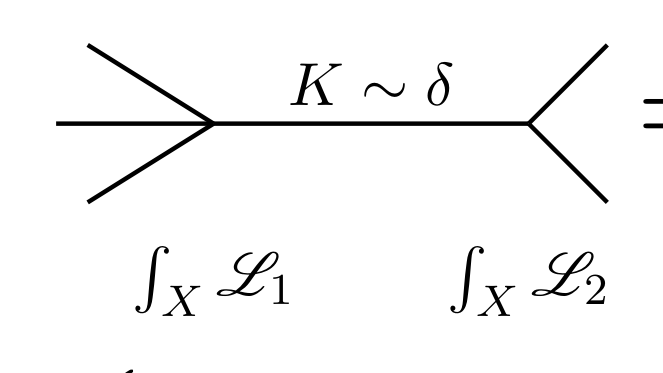
\includegraphics[width=0.27\linewidth]{fig_p063_1.png}
  \caption*{局部泛函上 BV 括号的缩并图示（原文 PDF p.63 示意图，原文无编号）}
\end{figure}
由此我们看到：经典主方程对局部泛函有意义，而量子主方程则需要重整化。

% [Tutor Note: 省略论证点拨——为什么 $\{-,-\}$ 在局部泛函上有定义？因为两个局部
% 泛函的 BV 括号只涉及有限阶导数（$\delta$-函数与其中一个泛函的导数缩并后仍为
% 局部表达式），而 $\Delta$ 需要对两个分布作缩并（即取 $K$ 与两个泛函的乘积），
% 在 $X$ 的对角线附近发散。故 CME 可写而 QME 不可写——这是本章全部技术工作的
% 出发点。]

% >>> p064

\begin{wexam}{7.3}（Chern--Simons 理论）
  取 $\mathcal{E}=\Omega^{\bullet}(X,\mathfrak{g})[1]$：
  \begin{center}
    \begin{tabular}{lcccc}
      \toprule
       & $\Omega^0(X,\mathfrak{g})$ & $\Omega^1(X,\mathfrak{g})$
       & $\Omega^2(X,\mathfrak{g})$ & $\Omega^3(X,\mathfrak{g})$\\
      \midrule
      次数 & $-1$ & $0$ & $1$ & $2$\\
      场 & $c$ & $A$ & $A^{\vee}$ & $c^{\vee}$\\
      物理 & 鬼场 & 场 & 反场 & 反鬼场\\
      \bottomrule
    \end{tabular}
  \end{center}
  设 $\mathcal{A}=C+A+A^{\vee}+C^{\vee}\in\mathcal{E}$ 为汇集全部分量的
  \textbf{主场}（master field）。则 BV Chern--Simons 作用量为
  \[
    \mathrm{CS}[\mathcal{A}]=\int_X\Tr\left(\frac{1}{2}\mathcal{A}\wedge \dd\mathcal{A}
    +\frac{1}{6}\mathcal{A}\wedge[\mathcal{A},\mathcal{A}]\right).
  \]
  这与通常的 Chern--Simons 形式相同，只是需要把 $\mathcal{A}$ 展开以得到含不同
  分量的项。第一个二次项记为 $S_{\mathrm{free}}$，即自由部分；第二个三次项记为
  $I$，即相互作用部分。
\end{wexam}

\begin{wprop}{7.4}
  $\mathrm{CS}$ 满足如下经典主方程
  \[
    \{\mathrm{CS},\mathrm{CS}\}=0.
  \]
\end{wprop}

\begin{proof}
  这源于“经典规范理论可组织为经典主方程的解”这一一般性论证。
\end{proof}

若把自由部分与相互作用部分分开
\[
  \mathrm{CS}=S_{\mathrm{free}}+I,
\]
则容易看出
\[
  \{S_{\mathrm{free}},-\}=\dd\ (=Q),
\]
这恰对应 de Rham 微分。于是
\[
  \begin{aligned}
    \{\mathrm{CS},\mathrm{CS}\}=0
    &\iff \frac{1}{2}\{S_{\mathrm{free}},S_{\mathrm{free}}\}
      +\{S_{\mathrm{free}},I\}+\frac{1}{2}\{I,I\}=0\\
    &\iff QI+\frac{1}{2}\{I,I\}=0.
  \end{aligned}
\]
这恰是我们 DGBV 中经典主方程的形式。

% [Tutor Note: 术语依据——master field 译“主场”（有的文献译“主字段”），
% 指把鬼场 $c$、场 $A$、反场 $A^{\vee}$、反鬼场 $c^{\vee}$ 合并成的单一分次对象
% $\mathcal{A}$；Chern--Simons 作用量对 $\mathcal{A}$ 仍取通常形式，展开后才显现
% 出各分量的耦合。原文全篇排作 Chern-Simons（单连字符），本译本统一用
% Chern--Simons。]

% >>> p065

\subsection{有效重整化（Effective Renormalization）}

假设有一个经典场论 $(\mathcal{E}=\Gamma(X,E^{\bullet}),Q,\omega)$，其经典局部泛函
$I_0$（相互作用）满足经典主方程
\[
  QI_0+\frac{1}{2}\{I_0,I_0\}=0.
\]
如我们先前所述，量子化要求
\[
  I_0\longmapsto I=I_0+\hbar I_1+\hbar I_2+\cdots
  \in\mathcal{O}(\mathcal{E})[[\hbar]]
\]
满足量子主方程
\[
  QI_0+\frac{1}{2}\{I_0,I_0\}+\hbar\Delta I=0.
\]
问题在于：$\Delta I$ 不是良定义的。下面我们解释 Costello 的同伦重整化理论
（homotopic renormalization theory），以解决这一问题。

% [Tutor Note: 原文用引号把上式标出，提示这只是形式上的写法（因为 $\Delta I$
% 无定义）；它应被理解为“把经典主方程逐阶 $O(\hbar)$ 修正”的启发式表达，而不是
% 严格等式。另，原文 “homotopic renormalization theory” 中 homotopic 一词，
% 学界亦常写作 homotopical/homotopy renormalization，译“同伦重整化理论”。]

\paragraph{玩具模型}

为启发该构造，让我们回顾玩具模型：$(V,Q,\omega)$ 是有限维 $(-1)$-平移 dg 辛空间，
Poisson 核
\[
  K_0\in\Sym^2(V)
\]
满足 $\deg(K_0)=1$ 且 $Q(K_0)=0$。这使我们能够通过与 $K_0$ 缩并来构造 BV 算子
$\Delta_0$，并得到 DGBV 三元组 $(A,Q,\Delta_0)$。

现在考虑用链同伦改变 $K_0$。设
\[
  P\in\Sym^2(V),\qquad \deg(P)=0.
\]
定义
\[
  K_P=K_0+Q(P)=K_0+(Q\otimes1+1\otimes Q)P.
\]
我们仍有
\begin{enumerate}[label=\textcircled{\small\arabic*},leftmargin=2.4em,itemsep=0.15em]
  \item $K_P\in\Sym^2(V)$，$\deg(K_P)=1$；
  \item $Q(K_P)=0$。
\end{enumerate}
因此可以构造新的 BV 算子 $\Delta_P$（即与 $K_P$ 缩并），使得
$(\mathcal{O}(V),Q,\Delta_P)$ 构成新的 DGBV。

为看清它与原 DGBV 的关系，记
\[
  \partial_P:\ \Sym^m(V^{\vee})\longrightarrow\Sym^{m-2}(V^{\vee}),
\]
其中 $\partial_P$ 是与 $P\in\Sym^2(V)$ 缩并的二阶算子。

\begin{wprop}{7.5}
  如下图表交换
  \begin{figure}[htbp]
  \centering
  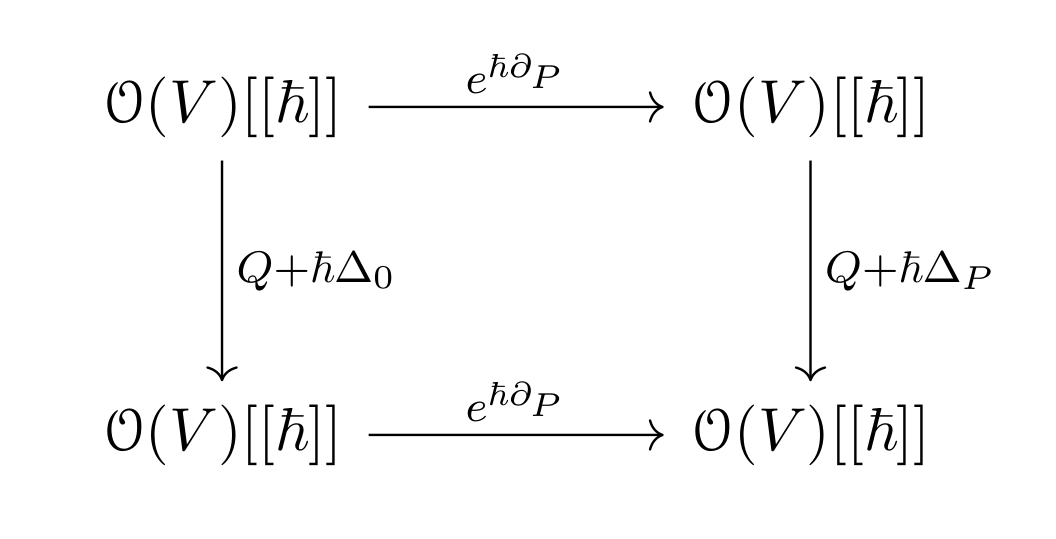
\includegraphics[width=0.42\linewidth]{fig_p065_1.png}
  \caption*{命题 7.5 的交换图表（原文 PDF p.65 示意图，原文无编号）}
\end{figure}
  即
  \[
    (Q+\hbar\Delta_P)\ee^{\hbar\partial_P}
    =\ee^{\hbar\partial_P}(Q+\hbar\Delta_0).
  \]
\end{wprop}

\begin{proof}
  这由链同伦关系 $K_P=K_0+Q(P)$ 推出。
\end{proof}

\begin{wcor}{7.6}
  假设 $I\in\mathcal{O}(V)[[\hbar]]$ 在 DGBV $(\mathcal{O}(V),Q,\Delta_0)$ 中满足
  量子主方程
  \[
    (Q+\hbar\Delta_0)\ee^{I/\hbar}=0.
  \]
  则 $\widetilde{I}\in\mathcal{O}(V)[[\hbar]]$ 在 DGBV
  $(\mathcal{O}(V),Q,\Delta_P)$ 中满足量子主方程
  \[
    (Q+\hbar\Delta_P)\ee^{\widetilde{I}/\hbar}=0.
  \]
  这里 $\widetilde{I}$ 与 $I$ 的关系为
  \[
    \ee^{\widetilde{I}/\hbar}=\ee^{\hbar\partial_P}\ee^{I/\hbar}.
  \]
\end{wcor}

% >>> p066

正如我们在 Feynman 图的讨论中所见，算子 $\ee^{\hbar\partial_P}$ 扮演对 Gaussian
测度积分的角色。关系 $\ee^{\widetilde{I}/\hbar}
=\ee^{\hbar\partial_P}\ee^{I/\hbar}$ 可按 Wick 定理读作
\begin{figure}[htbp]
  \centering
  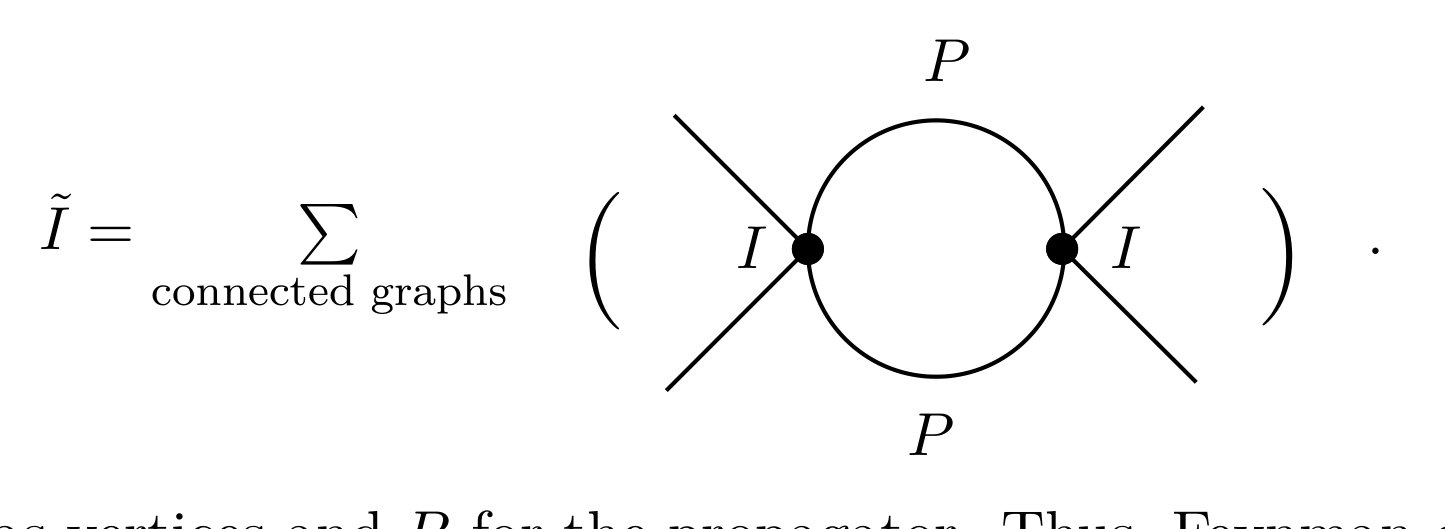
\includegraphics[width=0.58\linewidth]{fig_p066_1.png}
  \caption*{$\widetilde{I}$ 的连通图展开（原文 PDF p.66 示意图，原文无编号）}
\end{figure}
这里 $I$ 充当顶点，$P$ 充当传播子。于是，Feynman 图给出了不同 DGBV 之间所需的
链同伦。

% [Tutor Note: 省略论证 + 物理图像——（i）命题 7.5 的交换性证明被原文以
% “This follows from...” 一句带过：验证时只需注意 $\partial_P$ 是与 $P$ 缩并的
% 二阶算子，而 $\Delta_P-\Delta_0$ 是与 $Q(P)$ 缩并的算子，利用 $\Delta$ 与
% $\partial$ 的交换关系（符号由次数决定）即可把 $Q(P)$ 的贡献整理成
% $[Q,\cdot]$ 的交换子。（ii）$\ee^{\hbar\partial_P}$ 展开后给出所有可能的 Wick
% 收缩（即把若干 $I$ 的场按 $P$ 配对），连通图部分正是 $\widetilde{I}$ 的 Feynman
% 图展开。这一步把 5.1–5.2 节的 Wick 定理与图展开“翻译”成 BV 语言：换核
% $K_0\to K_P$ 相当于“积掉”由 $P$ 描述的高能自由度，这正是重整化的有限维模型。]

\paragraph{回到 QFT}

现在考虑 QFT 的设定 $(\mathcal{E}=\Gamma(X,E^{\bullet}),Q,\omega)$。问题在于
Poisson 核 $K_0=\omega^{-1}$ 是 $\delta$-函数分布，这导致 BV 算子奇异。不过我们知道
$K_0$ 是 $Q$-闭的：
\[
  Q(K_0)=0.
\]

\underline{Costello 的方法}：利用椭圆正则性
\[
  H^{\bullet}(\text{Distribution},Q)=H^{\bullet}(\text{Smooth},Q).
\]
于是我们可以把 $K_0$ 替换为其 $Q$-上同调类中的光滑对象：
\[
  K_0=K_r+Q(P_r).
\]
这里 $K_r$ 光滑，而 $P_r$（称为\textbf{参数化子}（parametrix））是奇异的。定义
$\Delta_r$ 为与 $K_r$ 相伴的 BV 算子。由于 $K_r\in\Sym^2(\mathcal{E})$ 现在是
光滑的，$\Delta_r$ 作用在 $\mathcal{O}(\mathcal{E})$ 上良定义。

% [Tutor Note: 省略论证点拨——$H^{\bullet}(\text{Distribution},Q)
% =H^{\bullet}(\text{Smooth},Q)$ 是椭圆正则性的推论：椭圆复形的上同调类总可用
% 光滑（甚至 $C^\infty$）代表元实现，因此可以用光滑的 $K_r$ 代表奇异的
% $\delta$-函数核；$P_r$ 只需作为“把两者联系起来的链同伦”存在，不必光滑
% （事实上它奇异，这正是 UV 发散的来源）。这是 Costello 同伦重整化的关键一步。]

\begin{wdefn}{7.7}
  DGBV $(\mathcal{O}(\mathcal{E}),Q,\Delta_r)$ 称为关于正则化 $r$ 的
  \textbf{有效 DGBV}（effective DGBV）。
\end{wdefn}

设 $r'$ 是另一个带有参数化子 $P_{r'}$ 的正则化：
\[
  K_0=K_{r'}+Q(P_{r'}).
\]
则两个正则化的 Poisson 核相差一个链同伦
\[
  K_{r'}-K_r=Q(P^{r'}_r),
\]
其中 $P^{r'}_r\in\Sym^2(\mathcal{E})$ 是光滑的。令
\[
  \partial_{P^{r'}_r}:\ \mathcal{O}(\mathcal{E})\longrightarrow\mathcal{O}(\mathcal{E})
\]
为与光滑核 $P^{r'}_r$ 缩并的二阶算子。与玩具模型中相同的论证给出链同伦
（下图中箭头即同伦重整化群流）：
\begin{figure}[htbp]
  \centering
  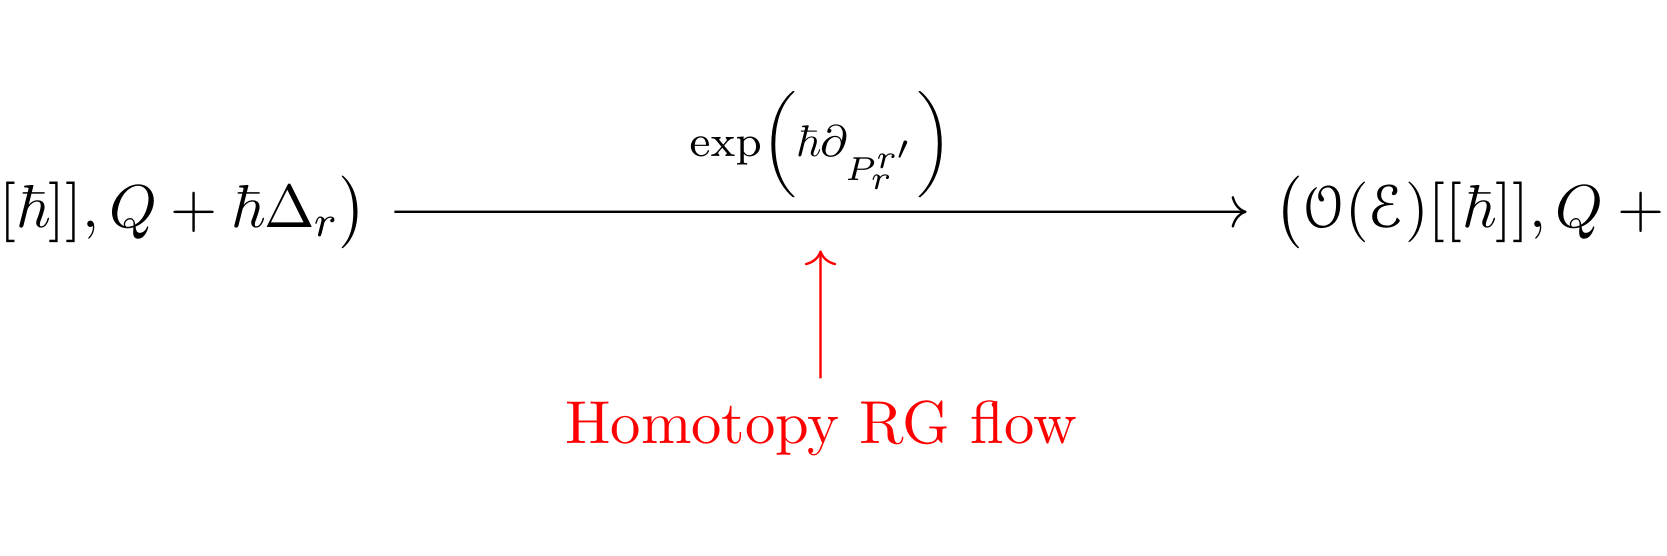
\includegraphics[width=0.67\linewidth]{fig_p066_2.png}
  \caption*{同伦重整化群流（原文 PDF p.66 示意图，原文无编号）}
\end{figure}

% >>> p067

\begin{wdefn}{7.8}（Costello）
  所谓 $I_0$（满足经典主方程）的\textbf{有效微扰量子化}，是指对每个正则化 $r$ 的
  选择给出一族
  \[
    I[r]\in\mathcal{O}(\mathcal{E})[[\hbar]],
  \]
  使得
  \begin{itemize}[leftmargin=1.6em,itemsep=0.3em]
    \item \textbf{有效主方程}
      \[
        (Q+\hbar\Delta_r)\ee^{I[r]/\hbar}=0;
      \]
    \item \textbf{同伦 RG 流}
      \[
        \ee^{I[r']/\hbar}=\ee^{\hbar\partial_{P^{r'}_r}}\ee^{I[r]/\hbar},
      \]
      这等价于 Feynman 图展开
      \begin{figure}[htbp]
  \centering
  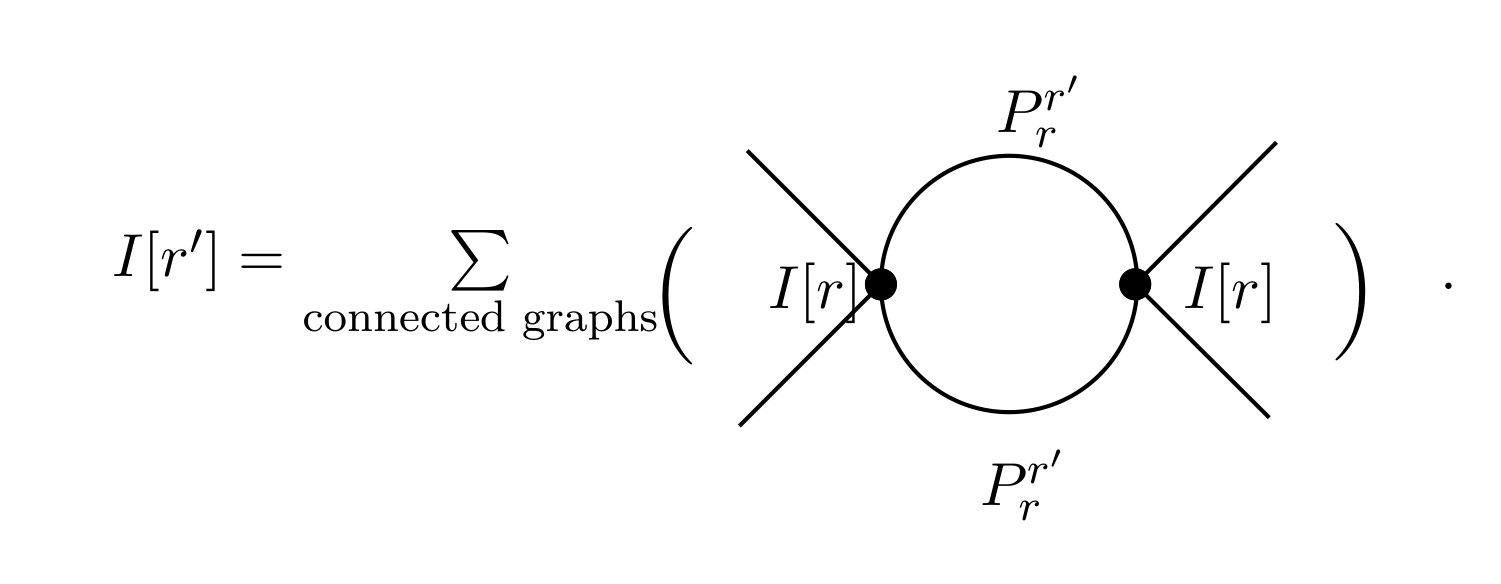
\includegraphics[width=0.60\linewidth]{fig_p067_1.png}
  \caption*{$I[r']$ 的连通图展开（原文 PDF p.67 示意图，原文无编号）}
\end{figure}
    \item $I[r]$ 当 $r\to 0$ 时是渐近局部的，并且有经典极限
      \[
        \lim_{r\to0}I_0[r]=I_0.
      \]
  \end{itemize}
\end{wdefn}

% [Tutor Note: 记号方向与原文疑误——（i）传播子 $P^{r'}_r$ 的上标 $r'$、下标 $r$
% 表示“从正则化 $r$ 到 $r'$”的链同伦；由 $K_{r'}-K_r=Q(P^{r'}_r)$ 可知方向是
% $r\to r'$。不同文献对上下标的方向约定不一，引用时务必与
% $\ee^{I[r']/\hbar}=\ee^{\hbar\partial_{P^{r'}_r}}\ee^{I[r]/\hbar}$ 互相校验。
% （ii）定义 7.8 首句 “An effective perturbative quantization of $I_0$ (which
% satisfies CME) a family $I[r]$...” 缺少谓语（应为 “is a family”），属笔误；
% 译文按语义补足为“是指……给出一族”。又，第三条中 $I_0[r]$ 的下标 $0$ 表示其
% $O(\hbar^0)$ 部分，与 $I[r]$ 的记号不同，切勿混读。]

下面这张图用来说明正在发生什么。情形与代数几何中留数（residue）的定义非常相似：
我们需要扰动奇点，在变形后的构型处定义留数，并说明所有的局部变形给出相同的答案。
这里我们用所有“邻近”的正则化来定义未重整化的点。
\begin{figure}[htbp]
  \centering
  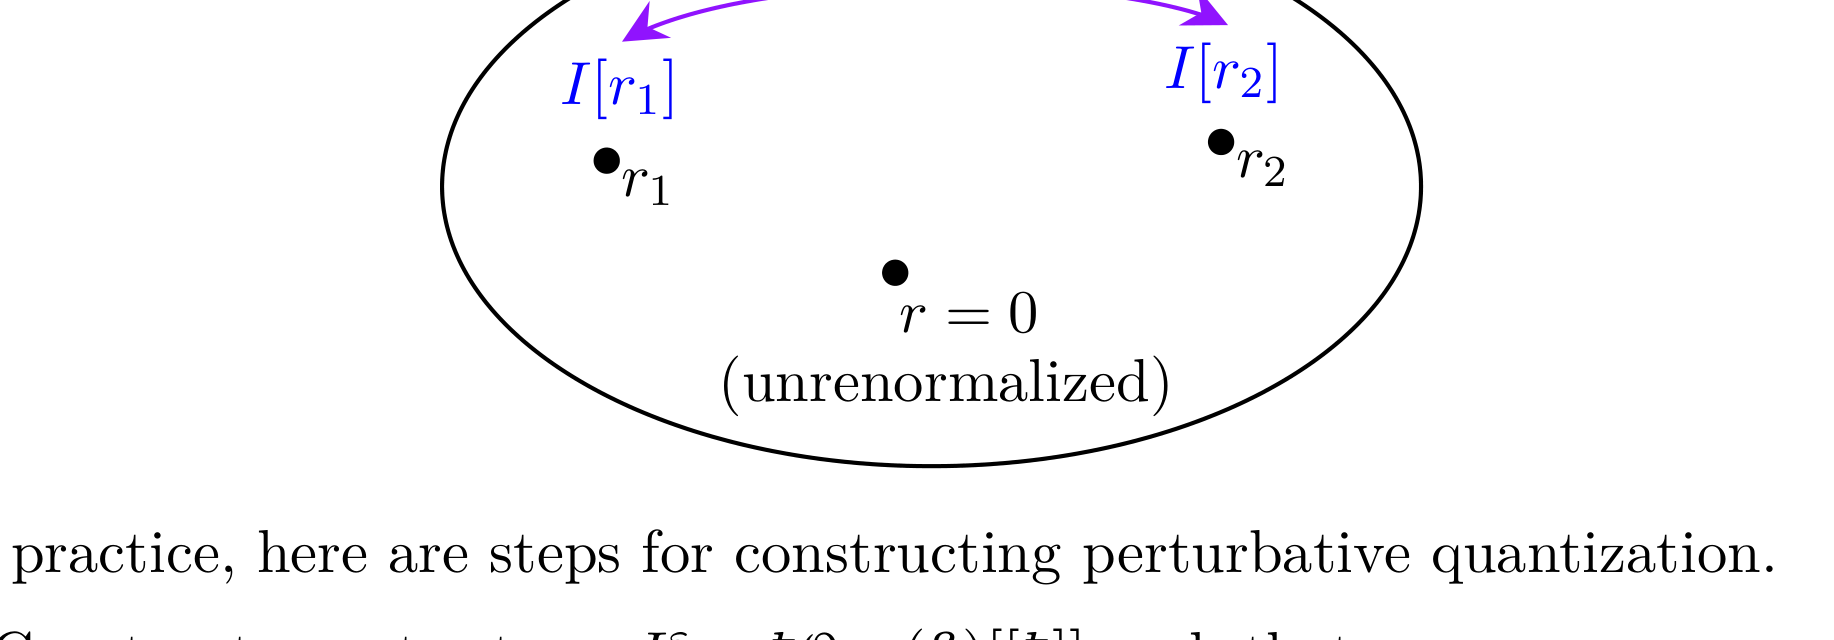
\includegraphics[width=0.74\linewidth]{fig_p067_2.png}
  \caption*{以邻近正则化定义未重整化点（原文 PDF p.67 示意图，原文无编号）}
\end{figure}

实际构造微扰量子化的步骤如下。
\begin{enumerate}[label=\textcircled{\small\arabic*},leftmargin=2.4em,itemsep=0.3em]
  \item 构造抵消项 $I^{\varepsilon}\in\hbar\mathcal{O}_{loc}(\mathcal{E})[[\hbar]]$，
        使得
        \[
          \ee^{I[r]^{\mathrm{Naive}}/\hbar}
          :=\lim_{\varepsilon\to0}
          \left(\ee^{\hbar P^r_{\varepsilon}}\ee^{(I_0+I^{\varepsilon})/\hbar}\right)
        \]
        存在。于是这个朴素族 $\{I[r]^{\mathrm{Naive}}\}_r$ 按构造满足同伦 RG 流。
  \item 抵消项的选取并不唯一。我们需要进一步修正 $I^{\varepsilon}$，使得
        $\ee^{I[r]/\hbar}$ 满足量子主方程。
\end{enumerate}
第 \textcircled{\small 1} 步总可以用抵消项方法做到；第 \textcircled{\small 2} 步则
并不总能做到：可能存在障碍，这在物理术语中称为“规范反常”（gauge anomaly）。
正如我们在形变–障碍理论的讨论中所见，类似的故事在此适用，规范反常位于
\[
  H^1(\mathcal{O}_{loc}(\mathcal{E}),Q+\{I_0,-\}).
\]

% [Tutor Note: 易错预警——第 ② 步是全书反复出现的“障碍”图景：抵消项（局部、
% 有限项）只能消去 UV 发散，但无法消除上同调类；障碍类住在
% $H^1(\mathcal{O}_{loc}(\mathcal{E}),Q+\{I_0,-\})$ 中，这与 6.6 节的
% $H^1(A,\delta)$ 完全平行（把 $A$ 换成 $\mathcal{O}_{loc}(\mathcal{E})$、
% $\delta$ 换成 $Q+\{I_0,-\}$）。另，原文 “Just as we have is the discussion of
% deformation-obstruction theory” 语法有误（多出 is），译文按原意处理。]

% >>> p068

\subsection{热核正则化（Heat Kernel Regularization）}

正则化的方式有很多。其中一种与几何相联系的方法是\textbf{热核正则化}。通常，
固定度量的选取后，我们有
\begin{itemize}[leftmargin=1.6em,itemsep=0.2em]
  \item 椭圆算子 $Q:\mathcal{E}\to\mathcal{E}$ 的伴随，记为
        $Q^{\dagger}:\mathcal{E}\to\mathcal{E}$；
  \item 广义 Laplacian
        \[
          [Q,Q^{\dagger}]=QQ^{\dagger}+Q^{\dagger}Q.
        \]
\end{itemize}
于是对 $L>0$ 可以定义热算子 $\ee^{-L[Q,Q^{\dagger}]}$。设
$K_L\in\Sym^2(\mathcal{E})$ 是热算子的核，即
\[
  \left(\ee^{-L[Q,Q^{\dagger}]}\alpha\right)(x)
  =\int \dd y\,\langle K_L(x,y),\alpha(y)\rangle,
  \qquad \alpha\in\mathcal{E}.
\]
这里 $\langle-,-\rangle$ 是由 $\omega$ 给出的配对。注意
\begin{itemize}[leftmargin=1.6em,itemsep=0.2em]
  \item $K_0=\lim_{L\to0}K_L$ 是 $\delta$-函数分布 $\omega^{-1}$；
  \item 对 $L>0$，$K_L\in\Sym^2(\mathcal{E})$ 光滑。
\end{itemize}

设 $P_L$ 是算子 $\int_0^L \dd t\,Q^{\dagger}\ee^{-t[Q,Q^{\dagger}]}$ 的核。具体地，
我们有
\[
  P_L=\int_0^L \dd t\,\left(Q^{\dagger}\otimes1\right)K_t.
\]
算子方程
\[
  \left[Q,\ \int_0^L \dd t\,Q^{\dagger}\ee^{-t[Q,Q^{\dagger}]}\right]
  =\int_0^L \dd t\,\left[Q,Q^{\dagger}\right]\ee^{-t[Q,Q^{\dagger}]}
  =1-\ee^{-L[Q,Q^{\dagger}]}
\]
可以翻译为核方程：
\[
  K_0-K_L=(Q\otimes1+1\otimes Q)P_L,
\]
或简写为
\[
  K_0-K_L=Q(P_L).
\]
我们可以用 $K_L$ 来定义有效量子主方程。

对 $0<\varepsilon<L$，类似地有算子方程
\[
  \left[Q,\ \int_{\varepsilon}^L \dd t\,Q^{\dagger}\ee^{-t[Q,Q^{\dagger}]}\right]
  =\ee^{-\varepsilon[Q,Q^{\dagger}]}-\ee^{-L[Q,Q^{\dagger}]},
\]
或者
\[
  K_{\varepsilon}-K_L=(Q\otimes1+1\otimes Q)P^L_{\varepsilon},
\]
其中 $P^L_{\varepsilon}
=\int_{\varepsilon}^L\dd t\,(Q^{\dagger}\otimes1)K_t$ 称为\textbf{正则化传播子}
（regularized propagator）。现在我们可以用 $P^L_{\varepsilon}$ 通过同伦 RG 流，
把 $\varepsilon$ 处的有效主方程与 $L$ 处的有效主方程联系起来。
\begin{figure}[htbp]
  \centering
  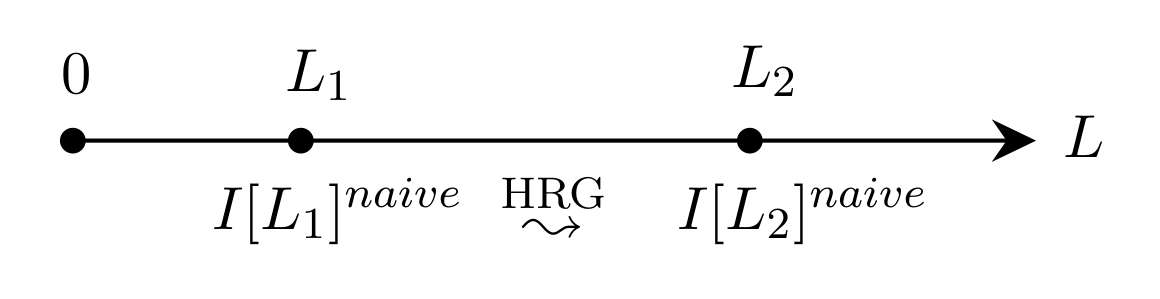
\includegraphics[width=0.47\linewidth]{fig_p068_1.png}
  \caption*{有效主方程随 $L$ 的同伦 RG 流（原文 PDF p.68 示意图，原文无编号）}
\end{figure}

% [Tutor Note: 符号与下标预警——（i）算子方程中 $\int_\varepsilon^L$ 的上下限
% 决定最后是 $\ee^{-\varepsilon[Q,Q^\dagger]}-\ee^{-L[Q,Q^\dagger]}$，差一个符号
% 就会把 $K_\varepsilon-K_L$ 写成 $K_L-K_\varepsilon$，务必按
% $-\frac{d}{dt}\ee^{-t[Q,Q^\dagger]}=[Q,Q^\dagger]\ee^{-t[Q,Q^\dagger]}$ 核对。
% （ii）$P_L$ 与 $P^L_\varepsilon$ 的下标/上标含义不同：$P_L$ 从 $0$ 积到 $L$
% （对应 $L$ 正则化）；$P^L_\varepsilon$ 从 $\varepsilon$ 积到 $L$
% （对应从 $\varepsilon$ 到 $L$ 的 HRG 流）。]

\begin{wrem}{7.9}
  $P^{\infty}_0=\int_0^{\infty}\dd t\,(Q^{\dagger}\otimes1)K_t$ 是\textbf{全传播子}
  （full propagator）。在 $t=0$ 处会遇到紫外（UV）发散，因为全传播子存在奇点。
  在非紧流形上，$t=\infty$ 处会遇到红外（IR）发散。
\end{wrem}

% >>> p069

考虑 $X$ 紧致的情形。设
\[
  \mathbb{H}=\left\{\varphi\in\mathcal{E}\ \middle|\ [Q,Q^{\dagger}]\varphi=0\right\}
  =\left\{\varphi\in\mathcal{E}\ \middle|\ Q\varphi=Q^{\dagger}\varphi=0\right\}
  \simeq H^{\bullet}(\mathcal{E},Q).
\]
$\mathbb{H}$ 称为\textbf{调和空间}（space of harmonics，或\textbf{零模}空间），
由 Hodge 理论它是有限维空间。于是我们有如下约化（下图示意了 $L\to\infty$
的极限）：
\begin{figure}[htbp]
  \centering
  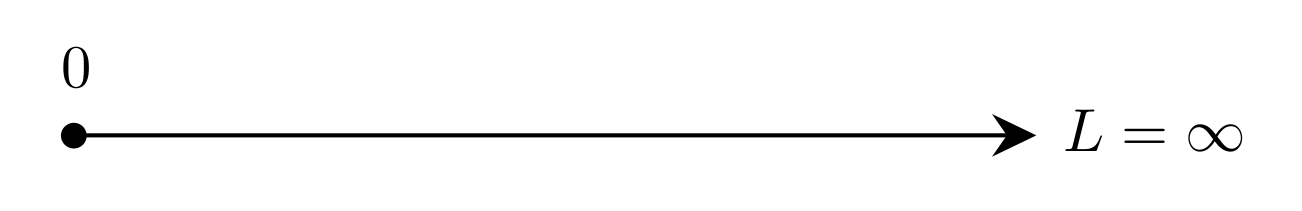
\includegraphics[width=0.52\linewidth]{fig_p069_1.png}
  \caption*{从无穷维 $(-1)$-辛几何到有限维 $(-1)$-辛几何的约化（原文 PDF p.69 示意图，原文无编号）}
\end{figure}
即 $L\to\infty$ 时，无穷维的 $(-1)$-辛几何 $(\mathcal{E},Q,\omega)$ 约化为有限维的
$(-1)$-辛几何 $(\mathbb{H},\omega_{\mathbb{H}}=\omega|_{\mathbb{H}})$。

与 $\omega^{-1}_{\mathbb{H}}$ 相伴的 BV 算子 $\Delta_H$ 是
$\Delta_H=\Delta_{\infty}$。关于 BV 量子化的完整图景如下图所示：
\begin{figure}[htbp]
  \centering
  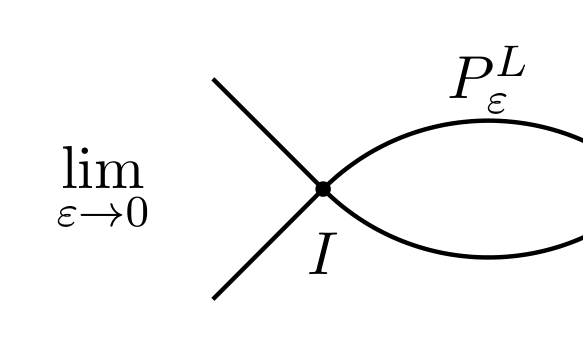
\includegraphics[width=0.23\linewidth]{fig_p069_2.png}
  \caption*{从 $0$ 到 $L=\infty$ 的 BV 量子化全图（原文 PDF p.69 示意图，原文无编号）}
\end{figure}
$I[\infty]$ 在 $L=\infty$ 处解 $(\mathcal{O}(\mathbb{H}),\Delta_H)$ 的量子主方程。
这是一个有趣的观点，我们从中会发现某些有限维的几何数据。

% [Tutor Note: 物理图像点拨——$L\to\infty$ 的极限把“所有高能模式”积掉，只剩下
% 调和空间 $\mathbb{H}$（零模）；此时 BV 算子 $\Delta_H$ 由
% $\omega^{-1}_{\mathbb{H}}$ 给出，是有限维、良定义的算子，于是 QME 变成一个
% 有限维问题。这正是 Hodge 分解
% $\mathcal{E}=\mathbb{H}\oplus\operatorname{im}Q\oplus\operatorname{im}Q^{\dagger}$
% 的量子场论意义，也是第 9、10 章“约化到有限维几何”的出发点。]

\subsection{UV 有限理论（UV Finite Theory）}

在 BV 形式中，经典主方程
\[
  QI_0+\frac{1}{2}\{I_0,I_0\}
\]
被量子化为量子主方程
\[
  QI+\hbar\Delta I+\frac{1}{2}\{I,I\}=0.
\]
如上面所解释的，这个朴素的量子主方程对局部
$I\in\mathcal{O}_{loc}(\mathcal{E})$ 是未定义的，我们必须用正则化来表述重整化后的
量子主方程
\[
  QI[r]+\hbar\Delta_r I[r]+\frac{1}{2}\{I,I\}_r=0.
\]
如果正则化 $r$ 处的有效作用量可以写成
\[
  \ee^{I[r]/\hbar}
  =\lim_{\varepsilon\to0}\ee^{\hbar\partial_{P^r_{\varepsilon}}}\ee^{I/\hbar},
\]
其中 $I\in\mathcal{O}_{loc}(\mathcal{E})[[\hbar]]$，即不需要依赖 $\varepsilon$ 的
抵消项，则称该理论是 \textbf{UV 有限的}（UV finite）。也就是说，对所有正则化的
Feynman 图
\begin{figure}[htbp]
  \centering
  
\includegraphics[width=0.29\linewidth]{fig_p069_3.png}
  \caption*{正则化 Feynman 图的 UV 极限（原文 PDF p.69 示意图，原文无编号）}
\end{figure}
相应的极限都存在。

% [Tutor Note: 术语依据——UV finite 译“UV 有限”（保留 UV 缩写，与 7.2 节
% “UV 问题”一致）。注意“不需要抵消项”不等于“没有发散”：是指所有正则化
% Feynman 图的 $\varepsilon\to0$ 极限本身存在，可用 $I\in\mathcal{O}_{loc}$
% 直接取极限，而不必先减去发散项。另，原文此处的 $\partial_{P^r_\varepsilon}$ 与
% 7.2 节的 $P^r_\varepsilon$ 记号一致，$\varepsilon\to0$ 对应移除截断。]

这样，我们可以考虑极限
\[
  I[r]\to I,\qquad r\to0,
\]
% >>> p070
以及重整化量子主方程的 $r\to0$ 极限
\[
  QI+\frac{1}{2}\{I,I\}+\cdots=0,
\]
它将具有一个使经典主方程发生形变的局部表达式。预期其形式为
\[
  l^{\hbar}_1I+\frac{1}{2}l^{\hbar}_2(I,I)+\frac{1}{3!}l^{\hbar}_3(I,I,I)
  +\cdots=0,
\]
其中 $\{l^{\hbar}_1,l^{\hbar}_2,\cdots\}$ 定义一个\textbf{量子化 $L_{\infty}$ 代数}
（quantized $L_\infty$-algebra），它可以视为在重整化过程中由 $\Delta$ 换取而来。

UV 有限理论主要有两大类。
\begin{enumerate}[label=\textcircled{\small\arabic*},leftmargin=2.4em,itemsep=0.25em]
  \item \textbf{拓扑理论}（Chern--Simons 型），其中 $\mathcal{E}$ 具有 de Rham
        复形的形式。见 Kontsevich \textup{[25]} 与 Axelrod--Singer \textup{[2]}。
  \item \textbf{全纯理论}，其中 $\mathcal{E}$ 具有 Dolbeault 复形的形式。
        $\dim_{\C}=1$ 的情形见 Li \textup{[28, 29]}，更高维的情形见 Wang \textup{[39]}。
\end{enumerate}

在这些例子中确定 $\{l^{\hbar}_1,l^{\hbar}_2,\cdots\}$ 是一个极其有趣的问题。
在第 9 章与第 10 章中，我们分别解释这两类中最简单的例子，以展示它们丰富的结构。

% [Tutor Note: 术语·文献依据与原文疑误——（i）$l^{\hbar}_1,l^{\hbar}_2,\cdots$ 是
% $L_\infty$ 结构映射（$l^{\hbar}_1$ 为微分，$l^{\hbar}_2$ 为括号，$l^{\hbar}_3$ 为
% 三阶运算……），方程中各项依次对应经典主方程的量子修正。（ii）原文
% “which can be viewed as traded from $\Delta$ in terms of the renormalization
% procedure” 中 “traded” 语义不清，疑为 “derived”（导出）或 “traced”（追踪）之
% 笔误，译文按字面作“换取而来”，请核对原书 p.69。（iii）方括号中的编号对应本书
% References（PDF p.101–103，见 part14.tex）：Kontsevich [25] 指其关于
% Chern–Simons 微扰量子化的拓扑不变量工作，Axelrod–Singer [2] 给出流形上链环的
% 微扰不变量；Li [28, 29] 与 Wang [39] 则是本书作者及其合作者关于全纯/手征理论的
% 工作。译文照录编号，读者请对照参考文献表查阅。]


% ---------- part10.tex ----------
% ============================================================
%  part10.tex  |  原文 PDF p.71–76（页脚 p.70–75）
%  内容：第 8 章 因子化代数（8.1 预因子化代数；8.2 因子化代数）
% ============================================================

% >>> p071
\section{因子化代数（Factorization Algebra）}

\begin{keypoints}
  \item \textbf{核心物理图像}：量子场论的可观测量并不附着于单个时空点，而是附着于
        时空开集 $U$：$\mathcal{F}(U)$ 是“支撑在 $U$ 内”的可观测量全体。当若干个两两
        不交的开集 $U_i$ 一同嵌入更大的开集 $V$ 时，可观测量的乘法（因子化乘积）给出
        映射 $\bigotimes_i\mathcal{F}(U_i)\to\mathcal{F}(V)$，这正是算子乘积展开（OPE）
        的公理化表述。
  \item \textbf{数学工具}：开集范畴 $\operatorname{Open}(M)$ 上的函子与余极限
        （$\operatorname{colim}$）、Weiss 覆盖与 Weiss 拓扑、余层（cosheaf）、
        \v{C}ech 复形；同伦版本则以拟同构代替正合性。
  \item \textbf{主要结论}：预因子化代数只要求因子化乘法的相容性；因子化代数则进一步
        要求 $\mathcal{F}$ 关于 Weiss 拓扑是余层。$\operatorname{Sym}(\Gamma_c(-,E))$
        给出最基本的因子化代数；微扰 BV 量子化产出（同伦）因子化代数，即“量子可观测量”。
  \item \textbf{译者评注}：本章把 1.2 节引入的“因子化乘积”公理化，是全书由微扰展开
        转向代数/拓扑观点的枢纽。8.2 节的 Weiss 覆盖解释了为何必须用比普通开覆盖更细的
        覆盖，也是第 9 章拓扑量子力学中局部—整体对应（HKR）的框架。
\end{keypoints}

\subsection{预因子化代数（Prefactorization Algebra）}

设 $M$ 是拓扑空间。记 $\operatorname{Open}(M)$ 为如下范畴：其对象是 $M$ 的开子集，
态射是开嵌入
\[
  U\longrightarrow V.
\]

\begin{wdefn}{8.1}
  取值于 $k$-向量空间范畴、定义在拓扑空间 $M$ 上的\emph{预因子化代数}
  （prefactorization algebra）$\mathcal{F}$ 是指一个函子
  \[
    \begin{aligned}
      \mathcal{F}:\ \operatorname{Open}(M)&\longrightarrow \Vect_k,\\
      U&\longmapsto \mathcal{F}(U),
    \end{aligned}
  \]
  连同对每一族两两不交的有限个开子集 $U_i\subset V$（即
  $U_1\sqcup\cdots\sqcup U_n\subset V$）给出的映射
  \[
    m^{U_1,\cdots,U_n}_{V}:\
    \mathcal{F}(U_1)\otimes\cdots\otimes\mathcal{F}(U_n)\longrightarrow\mathcal{F}(V),
  \]
  \begin{figure}[htbp]
  \centering
  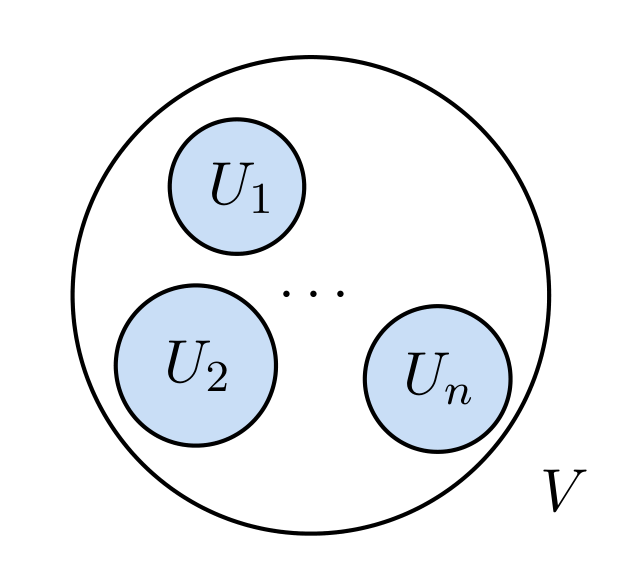
\includegraphics[width=0.25\linewidth]{fig_p071_1.png}
  \caption*{开集 $V$ 内互不相交的开子集 $U_1,\dots,U_n$（原文 PDF p.71 示意图，原文无编号）}
\end{figure}
  使得以下性质成立：
  \begin{enumerate}[label=(\arabic*),leftmargin=2.2em,itemsep=0.25em]
    \item 对 $U\subset V$，$m^{U}_{V}:\mathcal{F}(U)\to\mathcal{F}(V)$ 就是函子
          $\mathcal{F}$ 的态射。
    \item \textbf{相容性}：若 $U_{i,1}\sqcup\cdots\sqcup U_{i,n_i}\subset V_i$ 且
          $V_1\sqcup\cdots\sqcup V_k\subset W$，则下图交换：
          \[
            \begin{array}{ccc}
              \bigotimes_{i=1}^{k}\bigotimes_{j=1}^{n_i}\mathcal{F}(U_{i,j})
                & \longrightarrow & \bigotimes_{i=1}^{k}\mathcal{F}(V_i)\\[1mm]
              \searrow & & \big\downarrow\\[1mm]
              \multicolumn{3}{c}{\mathcal{F}(W)}
            \end{array}
          \]
          \begin{figure}[htbp]
  \centering
  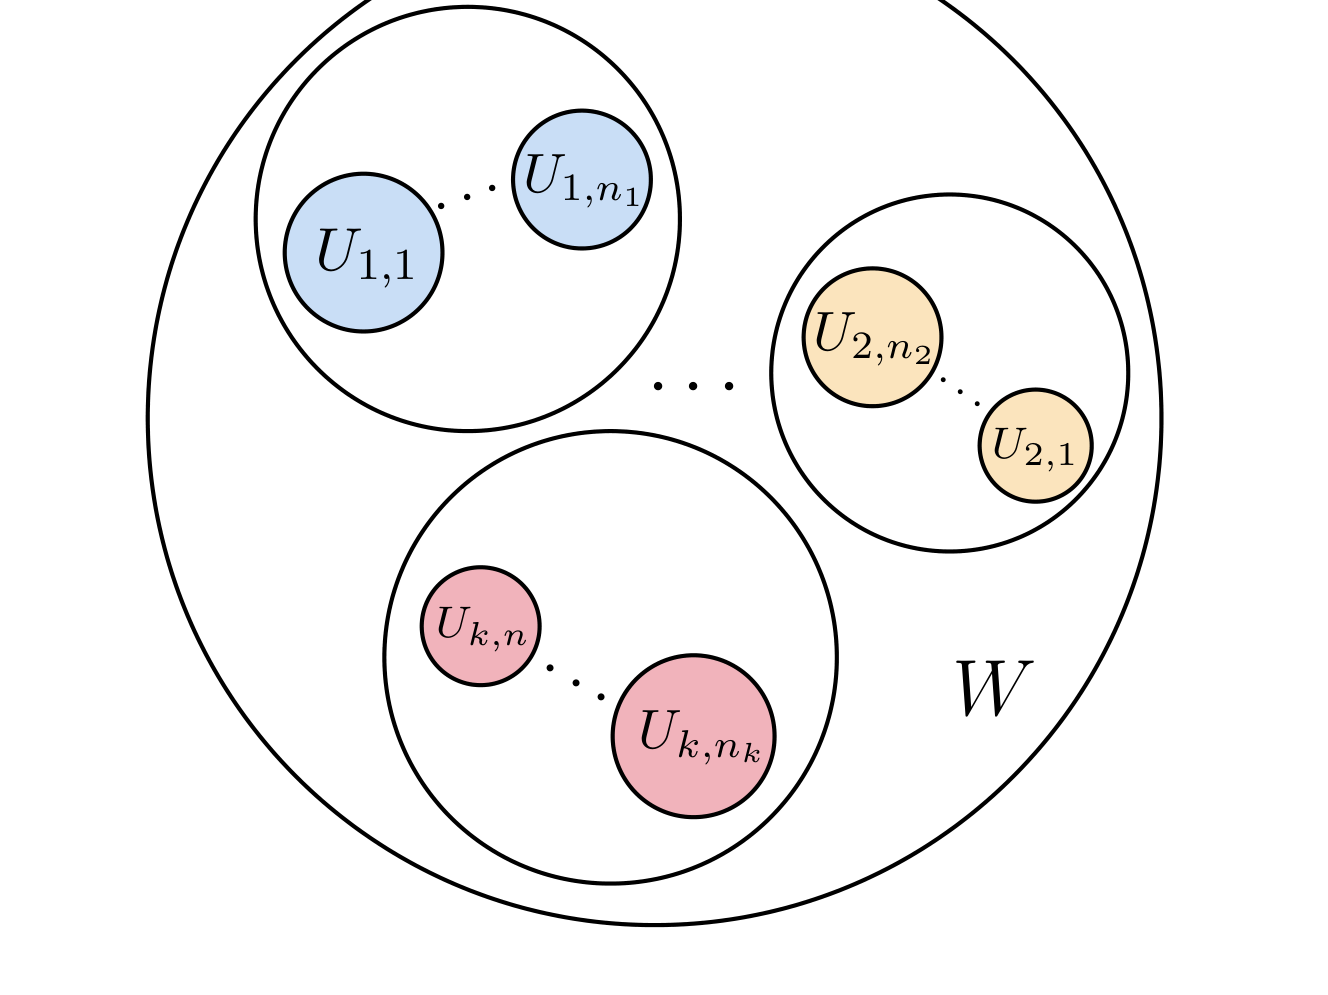
\includegraphics[width=0.53\linewidth]{fig_p071_2.png}
  \caption*{相容性条件所对应的嵌套开集（原文 PDF p.71 示意图，原文无编号）}
\end{figure}
  \end{enumerate}
\end{wdefn}

% [Tutor Note: 定义 8.1 中“函子 + 一族映射 $m^{U_1,\cdots,U_n}_V$”这两部分缺一不可：
% 函子性只给出“把 $U$ 嵌入 $V$”时的限制/延拓映射 $m^{U}_V$，而真正的代数结构来自
% 多变量的 $m^{U_1,\cdots,U_n}_V$。性质 (1) 只是说单变量情形与函子结构相容，
% 性质 (2) 才是结合律/交换律在因子化情形的替身。另注：原文 "valued in k-vector sapce"
% 中 "sapce" 显系 "space" 之笔误（PDF p.71），第 72 页 "unital commutative algerba"
% 亦然，均照译其义并注明。]

% >>> p072
由定义，空集上的 $\mathcal{F}(\varnothing)$ 是一个交换代数。若 $\mathcal{F}(\varnothing)$
是含幺交换代数，则称 $\mathcal{F}$ 为\emph{含幺预因子化代数}
（unital prefactorization algebra）。

% [Tutor Note: 为何 $\mathcal{F}(\varnothing)$ 自动是交换代数？空集只有唯一的分解——
% 即“空族”，故 $m^{\varnothing}_{\varnothing}:\mathcal{F}(\varnothing)\otimes
% \mathcal{F}(\varnothing)\to\mathcal{F}(\varnothing)$ 由公理给出；再把它与
% $\varnothing\sqcup\varnothing=\varnothing$ 的两种嵌套方式结合用相容性 (2)，
% 即得结合性与交换性。因此在例 8.2、例 8.4 中都有 $\mathcal{F}(\varnothing)=k$，
% 这些预因子化代数自动是含幺的。]

\begin{wexam}{8.2}
  设 $A$ 是含幺结合代数。我们如下在 $\R$ 上定义一个预因子化代数 $A^{fact}$。
  \begin{itemize}[leftmargin=1.8em,itemsep=0.35em]
    \item 对开区间 $(a,b)$，置
          \[
            A^{fact}((a,b))=A.
          \]
    \item 对开集 $\mathcal{U}=\bigsqcup_{j\in J}I_j$，其中 $I_j$ 为开区间，置
          \[
            A^{fact}(\mathcal{U})
              =\operatorname*{colim}_{\mathrm{finite}\,K\subset J}\ \bigotimes_{\alpha\in K}A.
          \]
          这里的余极限沿如下正向系统取：对任意有限指标集 $K\subset\tilde K$，
          \[
            \bigotimes_{K}A\longrightarrow\bigotimes_{\tilde K}A,
          \]
          该映射由张量上单位元 $1\in A$ 给出：
          \[
            \bigotimes_{\alpha\in K}a_k
              \longmapsto
            \Big(\bigotimes_{\alpha\in K}a_k\Big)\otimes
            \Big(\bigotimes_{\beta\in\tilde K-K}1\Big).
          \]
    \item 结构映射 $\{m^{U_1,\cdots,U_n}_{V}\}$ 由 $A$ 中的乘法给出：
          \begin{figure}[htbp]
  \centering
  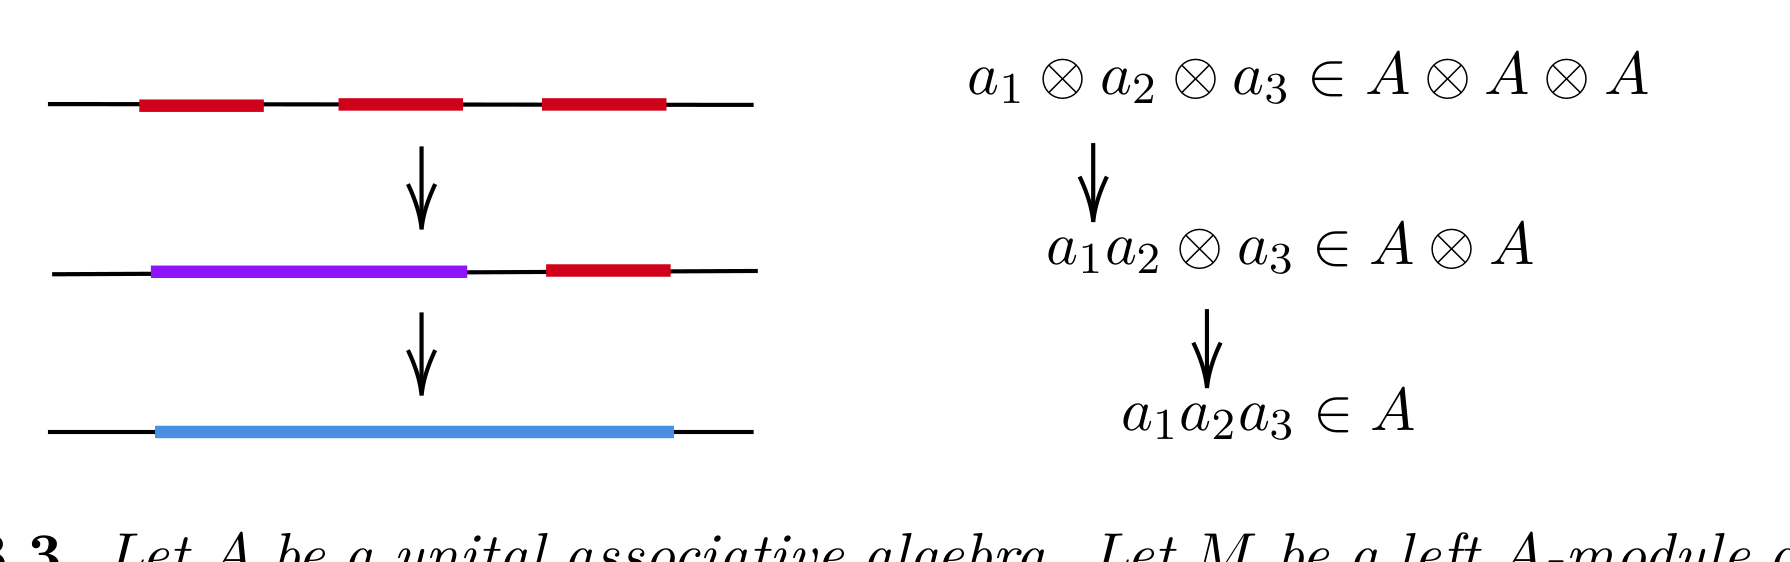
\includegraphics[width=0.72\linewidth]{fig_p072_1.png}
  \caption*{三个区间的逐次合并与结构映射（原文 PDF p.72 示意图，原文无编号）}
\end{figure}
          \[
            a_1\otimes a_2\otimes a_3\in A\otimes A\otimes A
            \ \longmapsto\
            a_1a_2\otimes a_3\in A\otimes A
            \ \longmapsto\
            a_1a_2a_3\in A.
          \]
  \end{itemize}
\end{wexam}

% [Tutor Note: 例 8.2 中“有限指标集 $K\subset J$ 上取余极限”是关键技术手段：若直接取
% 无穷张量积 $\bigotimes_{j\in J}A$，在 $J$ 无限时没有好定义；改为对有限子集取余极限，
% 相当于只允许“有限个区间上非平凡”的元素，这与紧支集截断的精神一致。
% 注意 $\bigotimes$ 取在 $k$ 上，故空张量积为 $k$，于是 $A^{fact}(\varnothing)=k$。
% 本例的意义是把“结合代数的乘法”分配到区间的合并过程上，是因子化代数最朴素的例子；
% 一般构造（因子化包络 factorization envelope）见 Costello--Gwilliam \textup{[11]}。
% 原文给出的 $a_k$ 上指标与求和指标 $\alpha$ 不一致（应为 $a_\alpha$），照录并请核对
% 原书 p.71（PDF p.72）。]

\begin{wexam}{8.3}
  设 $A$ 是含幺结合代数，$M$ 是左 $A$-模，$N$ 是右 $A$-模。我们可以如下在
  \[
    X=[0,1]
  \]
  上配置一个预因子化代数。
  \begin{itemize}[leftmargin=1.8em,itemsep=0.35em]
    \item 对 $U=\bigsqcup_{j\in J}I_j\subset(0,1)$，其中 $I_j$ 为开区间，对应
          \[
            \mathcal{F}(U)=\operatorname*{colim}_{\mathrm{finite}\,K\subset J}\
            \bigotimes_{\alpha\in K}A.
          \]
    \item 对 $U=U_1\sqcup U_2$，其中 $U_1\subset(0,a)$、$U_2=(a,1]$，有
          \begin{figure}[htbp]
  \centering
  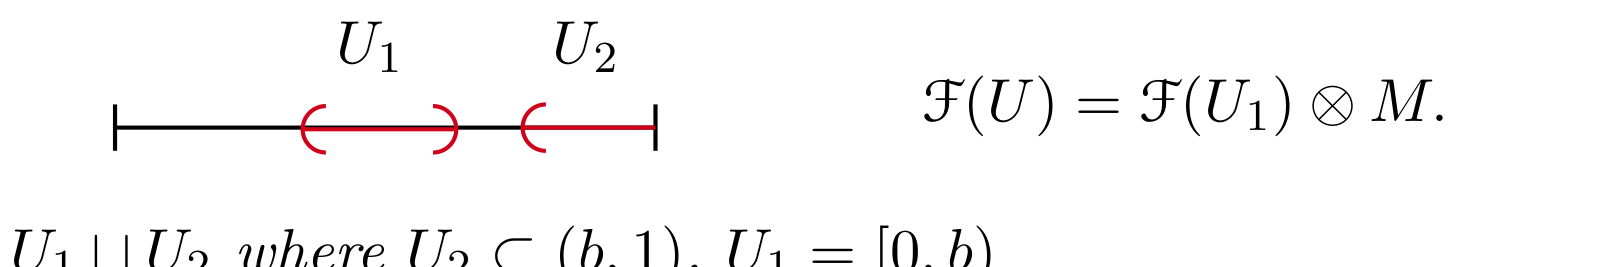
\includegraphics[width=0.65\linewidth]{fig_p072_2.png}
  \caption*{区间 $U_1\subset(0,a)$ 与 $U_2=(a,1]$ 的拼接（原文 PDF p.72 示意图，原文无编号）}
\end{figure}
          \[
            \mathcal{F}(U)=\mathcal{F}(U_1)\otimes M.
          \]
    \item 对 $U=U_1\sqcup U_2$，其中 $U_2\subset(b,1)$、$U_1=[0,b)$，有
          \begin{figure}[htbp]
  \centering
  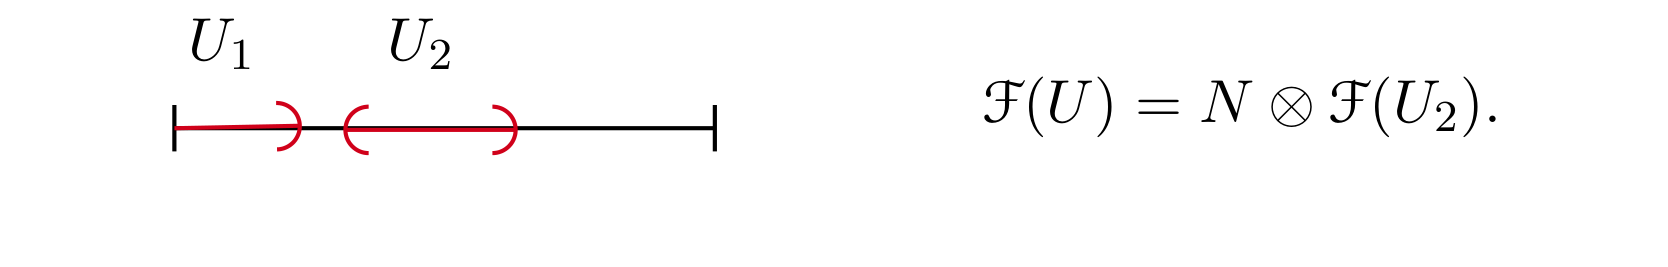
\includegraphics[width=0.67\linewidth]{fig_p072_3.png}
  \caption*{区间 $U_1=[0,b)$ 与 $U_2\subset(b,1)$ 的拼接（原文 PDF p.72 示意图，原文无编号）}
\end{figure}
          \[
            \mathcal{F}(U)=N\otimes\mathcal{F}(U_2).
          \]
    % [Tutor Note: 例 8.3 的端点归属极易看错：$U_1\subset(0,a)$ 是开区间，而
    % $U_2=(a,1]$ 含右端点 $1$；下一例中 $U_1=[0,b)$ 含左端点而 $U_2\subset(b,1)$
    % 是开区间。端点处的半开区间分别承载边界态 $M$（右端）与 $N$（左端），因此 $M$
    % 是左 $A$-模、$N$ 是右 $A$-模。这是“有边界的一维 QFT”中边界条件/边界可观测量
    % 的代数化身，符号一旦弄反，得到的就不是模作用而是反模作用。]

    % [Tutor Note: 原文 "We can associative a prefactorization on $X$" 中
    % "associative" 应为动词 "associate"（原文 PDF p.72），属笔误，照译并注明。]

% >>> p073
    \item 对 $U=U_1\sqcup U_2\sqcup U_3$，其中 $U_1=[0,a)$、$U_2\subset(a,b)$、
          $U_3=(b,1]$，有
          \begin{figure}[htbp]
  \centering
  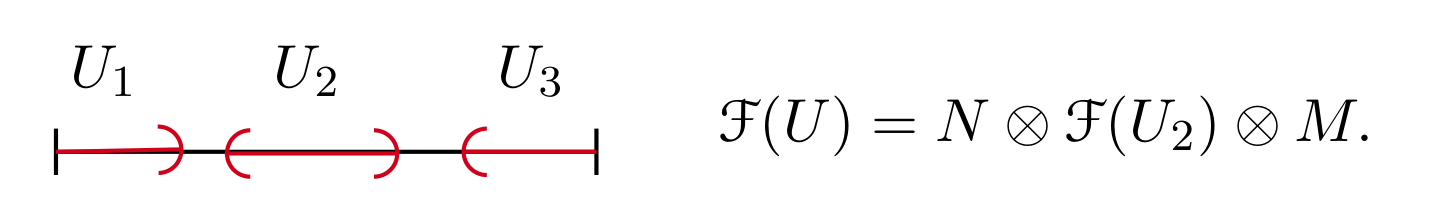
\includegraphics[width=0.57\linewidth]{fig_p073_1.png}
  \caption*{三段区间 $U_1=[0,a)$、$U_2\subset(a,b)$、$U_3=(b,1]$ 的拼接（原文 PDF p.73 示意图，原文无编号）}
\end{figure}
          \[
            \mathcal{F}(U)=N\otimes\mathcal{F}(U_2)\otimes M.
          \]
  \end{itemize}
\end{wexam}


\begin{wexam}{8.4}
  设 $E\to X$ 是 $X$ 上的向量丛。对每个开集 $U\subset X$，对应
  \[
    \mathcal{F}(U)=\operatorname{Sym}\big(\Gamma_c(U,E)\big).
  \]
  这里 $\Gamma_c(U,E)$ 是 $E$ 在 $U$ 内的紧支集截面。利用零延拓，对 $U\subset V$ 有
  \[
    \Gamma_c(U,E)\hookrightarrow\Gamma_c(V,E),
  \]
  它诱导
  \[
    \mathcal{F}(U)\hookrightarrow\mathcal{F}(V).
  \]
  对有限个两两不交的 $U_1\sqcup\cdots\sqcup U_n$，有
  \[
    \Gamma_c\Big(\bigsqcup_i U_i,E\Big)=\bigoplus_{i=1}^{n}\Gamma_c(U_i,E),
  \]
  并且
  \[
    \operatorname{Sym}\Big(\Gamma_c\big(\bigsqcup_i U_i,E\big)\Big)
    =\operatorname{Sym}\Big(\bigoplus_{i=1}^{n}\Gamma_c(U_i,E)\Big)
    =\bigotimes_{i=1}^{n}\operatorname{Sym}\big(\Gamma_c(U_i,E)\big).
  \]
  这表明
  \[
    \mathcal{F}\Big(\bigsqcup_{i=1}^{n}U_i\Big)=\bigotimes_{i=1}^{n}\mathcal{F}(U_i),
  \]
  于是我们得到一个预因子化代数。
\end{wexam}

% [Tutor Note: 例 8.4 的关键在于“紧支集”：$\Gamma_c$ 把不交并变成直和
% （$\Gamma_c(\bigsqcup U_i)=\bigoplus\Gamma_c(U_i)$），而 $\operatorname{Sym}$ 又把
% 直和变成张量积（$\operatorname{Sym}(V\oplus W)=\operatorname{Sym}V\otimes
% \operatorname{Sym}W$），两步合起来恰好给出因子化乘法的同构。若改用普通截面
% $\Gamma$，不交并对应的是直积而非直和，得到的将是层（sheaf）而非余层（cosheaf），
% 因子化性质随之失效。]

\begin{wdefn}{8.5}
  预因子化代数的态射
  \[
    \phi:\ \mathcal{F}\longrightarrow\mathcal{G}
  \]
  由一族映射 $\phi_U:\mathcal{F}(U)\to\mathcal{G}(U)$（对每个开集 $U\subset M$）组成，
  它们与结构映射相容，即下图交换：
  \[
    \begin{array}{ccc}
      \mathcal{F}(U_1)\otimes\cdots\otimes\mathcal{F}(U_n)
        & \xrightarrow{\ \phi_{U_1}\otimes\cdots\otimes\phi_{U_n}\ }
        & \mathcal{G}(U_1)\otimes\cdots\otimes\mathcal{G}(U_n)\\[1mm]
      \big\downarrow & & \big\downarrow\\[1mm]
      \mathcal{F}(V) & \xrightarrow{\ \phi_V\ } & \mathcal{G}(V)
    \end{array}
  \]
\end{wdefn}

于是预因子化代数构成一个范畴。

\subsection{因子化代数（Factorization Algebra）}

\begin{wdefn}{8.6}
  设 $U$ 是 $M$ 中的开集。$U$ 的开覆盖
  $\mathfrak{U}=\{U_i\subset U\}_{i\in I}$ 称为 \emph{Weiss 覆盖}（Weiss cover），
  如果对 $U$ 中任意有限点集 $\{x_1,\dots,x_k\}$，存在开集 $U_j\in\mathfrak{U}$
  使得 $\{x_1,\dots,x_k\}\subseteq U_j$。
\end{wdefn}

\begin{wprop}{8.7}
  若 $\mathfrak{U}=\{U_i\}$ 是 $U$ 的 Weiss 覆盖，则对任意 $n>0$，
  \[
    \{U_i^{n}\}_{i\in I}
  \]
  是 $U^{n}=U\times\cdots\times U$ 的开覆盖。
\end{wprop}

% [Tutor Note: Weiss 覆盖的定义要点在“任意\emph{有限}点集”而非“任意一点”——后者只是
% 普通开覆盖。取“能同时容纳任意有限个点”的开集，正是为了控制多点函数
% （即 $U^n$ 上的对象，如关联函数/多算子插入）的局部性。例 8.8 说明
% “$U$ 去掉有限个点”这种族已是 Weiss 覆盖，可见 Weiss 覆盖比普通开覆盖“更细、更灵活”。
% 术语依据：Weiss 覆盖得名于 M. Weiss 关于 manifold calculus 的工作；
% 中文文献多径直音译作“Weiss 覆盖”。]

% >>> p074
\begin{proof}
  对任意 $(x_1,\cdots,x_n)\in U^{n}$，存在 $U_i$，使得
  \[
    \{x_1,\cdots,x_k\}\subset U_i
    \ \Longrightarrow\
    (x_1,\cdots,x_n)\in U_i^{n}.
  \]
\end{proof}

% [Tutor Note: 命题 8.7 的证明中，原文把点集写成 $\{x_1,\cdots,x_k\}$，但按命题陈述与
% 上下文应为 $\{x_1,\cdots,x_n\}$（$k$ 是定义 8.6 中的点数，此处应取 $k=n$）；
% 这是原文的小失误，照录并请核对原书 p.73（PDF p.74）。]

\begin{wexam}{8.8}
  由“从 $U$ 中删去有限个点所得的集合”构成的族，是 $U$ 的一个 Weiss 覆盖。
\end{wexam}

\begin{wdefn}{8.9}
  若对每个开集 $U\subset M$ 与 $U$ 的每个 Weiss 覆盖
  $\mathfrak{U}=\{U_i\}_{i\in I}$，下述序列正合：
  \[
    \bigoplus_{i,j}\mathcal{F}(U_i\cap U_j)
    \longrightarrow
    \bigoplus_{k}\mathcal{F}(U_k)
    \longrightarrow
    \mathcal{F}(U)
    \longrightarrow 0,
  \]
  则称 $M$ 上的预因子化代数 $\mathcal{F}$ 为\emph{因子化代数}
  （factorization algebra）。
\end{wdefn}

回忆：$M$ 上 $k$-向量空间的层（sheaf）$\mathcal{E}$ 是函子
\[
  \mathcal{E}:\ \operatorname{Open}(M)^{op}\longrightarrow \Vect_k,
\]
满足粘接条件：对 $U$ 的任意开覆盖 $\mathfrak{U}=\{U_i\}_{i\in I}$，
\[
  0\longrightarrow\mathcal{E}(U)
  \longrightarrow\bigoplus_{i\in I}\mathcal{E}(U_i)
  \longrightarrow\bigoplus_{i,j}\mathcal{E}(U_i\cap U_j)
\]
构成正合序列。这意味着 $\mathcal{E}(U)$ 的一个截面 $s$ 可以唯一地由每个 $U_i$ 上的
截面 $s_i$ 指定，只要它们在重叠处相符：
$s_i|_{U_i\cap U_j}=s_j|_{U_i\cap U_j}$。把箭头对偶化，我们就得到\emph{余层}
（cosheaf）的概念。

因此，预因子化代数 $\mathcal{F}$ 是因子化代数，当且仅当它是关于 Weiss 拓扑的余层。

% [Tutor Note: 层与余层的差别只在箭头方向：层的粘接是“限制映射”+ 左端正合，
% 余层的粘接是“延拓映射”+ 右端以 $0$ 收尾。定义 8.9 的序列以 $\to 0$ 结尾、
% 开头没有 $0$，正是“余层”的特征；判断正合列该在哪一端加 $0$ 是本章最易出错处。
% 另注：$\bigoplus_{i,j}$ 是否包含 $i=j$ 项各文献约定不同，包含与否只差一些可缩项，
% 不影响正合性；此处按原文取遍所有 $i,j$。
% 又，“Weiss 拓扑”的严格含义是把 Weiss 覆盖取作 Grothendieck 拓扑的覆盖族
% （需验证 Weiss 覆盖对拉回与局部化封闭，构成预拓扑）。因此“关于 Weiss 拓扑的余层”
% 是一个标准的层论陈述，可与普通拓扑（开覆盖）下的层论逐条对照，差别只在覆盖族的大小。]

\begin{wexam}{8.10}
  设 $E\to X$ 是 $X$ 上的向量丛。记 $\mathcal{E}_c$ 为余层
  \[
    \mathcal{E}_c(U)=\Gamma_c(U,E),
  \]
  它把开集 $U$ 对应到其上的紧支集截面。记
  \[
    \mathcal{F}=\operatorname{Sym}(\mathcal{E}_c)
  \]
  为预因子化代数，其中
  \[
    \mathcal{F}(U)=\operatorname{Sym}(\mathcal{E}_c(U)).
  \]
  我们来证明 $\mathcal{F}$ 是因子化代数。设 $U\subset M$ 是开集，
  \[
    \mathfrak{U}=\{U_i\subset U\}_{i\in I}
  \]
  是 $U$ 的 Weiss 覆盖。我们需要证明
  \[
    \bigoplus_{i,j\in I}\operatorname{Sym}\big(\mathcal{E}_c(U_i\cap U_j)\big)
    \longrightarrow
    \bigoplus_{i\in I}\operatorname{Sym}\big(\mathcal{E}_c(U_i)\big)
    \longrightarrow
    \operatorname{Sym}\big(\mathcal{E}_c(U)\big)
    \longrightarrow 0
  \]
  正合。注意到
  \[
    \mathcal{E}_c(U)^{\hat\otimes m}=\mathcal{E}_c^{\boxtimes m}(U^{m}),
  \]
  其中 $\mathcal{E}_c^{\boxtimes m}$ 是 $U^{m}$ 上紧支集截面所成的余层 $E^{\boxtimes m}$。
  按每个张量分量分解，我们需要证明
  \[
    \bigoplus_{i,j\in I}\mathcal{E}_c^{\boxtimes m}(U_i\cap U_j))
    \longrightarrow
    \bigoplus_{i\in I}\mathcal{E}_c^{\boxtimes m}(U_i))
    \longrightarrow
    \mathcal{E}_c^{\boxtimes}(U)
    \longrightarrow 0
  \]
  正合。由于 $\{U_i\}_{i\in I}$ 是 Weiss 覆盖，$\{U_i^{m}\}_{i\in I}$ 构成 $U$ 的
  开覆盖，并且
  \[
    (U_i\cap U_j)^{m}=U_i^{m}\cap U_j^{m}.
  \]
  于是正合性由 $\mathcal{E}_c^{\boxtimes m}$ 在 $U^{m}$ 上的余层性质推出。
\end{wexam}

% [Tutor Note: 原文 "which assigns compactly sections on U" 应为 "compactly supported
% sections"（原文 PDF p.74）；另本段末尾两个求和中各多出一个右括号
% （原作 $\mathcal{E}_c^{\boxtimes m}(U_i\cap U_j))$、$\mathcal{E}_c^{\boxtimes m}(U_i))$），
% 且末项上标只印作 $\boxtimes$（疑漏 $m$，前两项均为 $\boxtimes m$）。三处均照录原文，
% 请核对原书 p.73（PDF p.74）。
% 又，这里 $\hat\otimes$ 表示张量积的完备化（在通常的拓扑/准完备设定下），
% 等式 $\mathcal{E}_c(U)^{\hat\otimes m}=\mathcal{E}_c^{\boxtimes m}(U^m)$ 说明
% “$U$ 上 $m$ 重张量幂”等于“$U^m$ 上的外积余层”；这一步是把 $m$ 次对称张量的问题
% 化到 $U^m$ 上、从而用命题 8.7 的关键。符号上 $\boxtimes$（外张量积）与
% $\otimes$（内张量积）不可混用。]

% >>> p075
更一般地，我们可以定义取值于上链复形的预因子化代数。于是对每个 $U\subset M$，
$\mathcal{F}(U)$ 是一个上链复形。对任意覆盖
$\mathfrak{U}=\{U_i\subset U\}_{i\in I}$，我们可以类似地定义 \v{C}ech 上链
\[
  C^{p}(\mathfrak{U},\mathcal{F})
  :=\bigoplus_{j_0,\dots,j_p\ \mathrm{distinct}}
  \mathcal{F}(U_{j_0}\cap\cdots\cap U_{j_p}),
\]
以及作为
\[
  \check{C}(\mathfrak{U},\mathcal{F})
  :=\bigoplus_{p=0}^{\infty}C^{p}(\mathfrak{U},\mathcal{F})
\]
的总复形的 \v{C}ech 复形。

\begin{wdefn}{8.11}
  \emph{同伦因子化代数}（homotopy factorization algebra）是指 $M$ 上的预因子化代数
  $\mathcal{F}$，使得对每个开集 $U\subset X$ 与 $U$ 的 Weiss 覆盖 $\mathfrak{U}$，
  自然映射
  \[
    \check{C}(\mathfrak{U},\mathcal{F})\longrightarrow\mathcal{F}(U)
  \]
  是拟同构。从而 $\mathcal{F}$ 是关于 Weiss 拓扑的同伦余层。
\end{wdefn}

% [Tutor Note: 同伦版本把定义 8.9 的“序列正合”升级为“\v{C}ech 复形与 $\mathcal{F}(U)$
% 拟同构”。实际计算时 $\check{C}(\mathfrak{U},\mathcal{F})$ 取总复形，其微分同时包含
% \v{C}ech 微分与 $\mathcal{F}(U_i)$ 自身的内部微分（例如 BV 算子 $Q$）；正因为如此，
% 对拟同构取同调后才得到物理上正确的“量子可观测量”。原文此处写 $U\subset X$，
% 而上下文底流形记为 $M$，属记号不一致，照录并请核对原书 p.74（PDF p.75）。]

在 Costello--Gwilliam \textup{[11]} 中证明了：微扰 BV 量子化导出（同伦）因子化代数。
这样的因子化代数描述“量子可观测量”，而因子化性质正是局部—整体性质。

% [Tutor Note: 原文作 "Costello-Gwillian"，应为 "Costello–Gwilliam"（Kevin Costello
% 与 Owen Gwilliam，原文 PDF p.75），属笔误，照译并注明。文献 [11] 即其两卷本
% \emph{Factorization Algebras in Quantum Field Theory}。]

\begin{wexam}{8.12}
  作为例子，考虑相空间 $\R^{2n}$ 上的拓扑量子力学（详见第 9 章）。场空间为
  \[
    \mathcal{E}=\Omega^{\bullet}(S^{1})\otimes\R^{2n}.
  \]
  给定 $U\subset S^{1}$，$U$ 内部的可观测量 $\Obs(U)$ 是
  \[
    \mathcal{E}(U)=\Omega^{\bullet}(U)\otimes\R^{2n}
  \]
  上的函数。
  \begin{itemize}[leftmargin=1.8em,itemsep=0.35em]
    \item \textbf{局部可观测量}：设 $U$ 是小开区间。
          \begin{figure}[htbp]
  \centering
  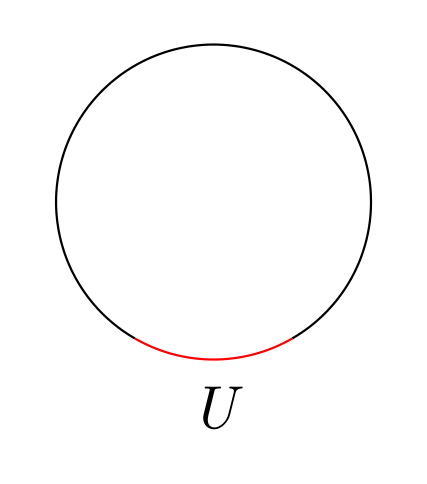
\includegraphics[width=0.22\linewidth]{fig_p075_1.png}
  \caption*{圆周 $S^1$ 上标出小开区间 $U$（原文 PDF p.75 示意图，原文无编号）}
\end{figure}
          由 Poincaré 引理，$\Omega^{\bullet}(U)\simeq\R$ 是拟同构的。于是
          \[
            \Obs(U)=O(\mathcal{E}(U))\simeq\mathcal{O}(\R^{2n})
            =\R[x^{i},p_i].
          \]
    \item \textbf{整体可观测量}：对 $U=S^{1}$，其同调非平凡：
          \[
            \Omega(S^{1})\simeq H^{\bullet}(S^{1})=\R\oplus\R[-1].
          \]
          于是 $S^{1}$ 上的整体可观测量可模型化为
          \[
            \Obs(S^{1})\simeq\mathcal{O}\big(\Omega(S^{1})\otimes\R^{2n}\big)
            \simeq\mathcal{O}\big(\R^{2n}\oplus\R^{2n}[-1]\big)
            \simeq\R[x^{i},p_i,\dd x^{i},\dd p_i].
          \]
  \end{itemize}
  局部可观测量 $\Obs(U)=\R[x^{i},p_i]$ 与整体可观测量
  $\Obs(S^{1})=\R[x^{i},p_i,\dd x^{i},\dd p_i]$ 之间的关系，恰是 Hochschild 同调
  （由 Hochschild--Kostant--Rosenberg（HKR）定理）。
  \[
    S^{1}\text{-factorization Homology}=\text{Hochschild Homology}.
  \]
\end{wexam}

% [Tutor Note: 例 8.12 中 $\R[x^i,p_i]$ 取的是\emph{多项式}函数而非光滑函数，
% 原因是 $\Omega^{\bullet}(U)\simeq\R$ 的拟同构把复形层面的信息压成同调，
% 可观测量复形因此与多项式函数环拟同构；这在 BV/形变量子化的代数框架中更便于计算。
% 另注意 $\R[-1]$ 表示同调次数下移一位（degree shift），故
% $\R^{2n}\oplus\R^{2n}[-1]$ 的两个直和项分别对应坐标 $x^i,p_i$ 与其微分
% $\dd x^i,\dd p_i$，这正是“整体可观测量比局部多出一倍生成元”的含义。
% 末行的 HKR 定理指：对光滑仿射代数（或其上的多项式代数），Hochschild 同调同构于
% 微分形式代数（Hochschild--Kostant--Rosenberg）；本例把它几何化为
% “$S^1$ 上的整体可观测量 = 局部可观测量的 Hochschild 同调”，亦即
% “因子化同调 = Hochschild 同调”。]

% >>> p076
在量子层面，局部可观测量成为 Weyl 代数
\[
  \mathcal{A}^{\hbar}=(\mathcal{A}[[\hbar]],\star),
\]
其中 $\star$ 是 Moyal 积。于是该模型中的量子关联函数（见定义 9.10）
\begin{figure}[htbp]
  \centering
  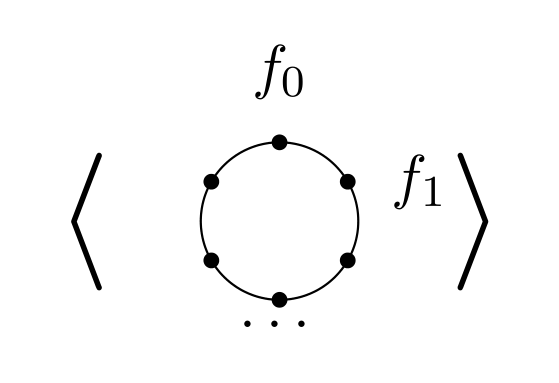
\includegraphics[width=0.22\linewidth]{fig_p076_1.png}
  \caption*{量子关联函数 $\langle f_0\cdots f_1\rangle$ 的圆环表示（原文 PDF p.76 示意图，原文无编号）}
\end{figure}
给出一个显式的链映射（Gui--Li--Xu \textup{[24]} 与 Li--Wang--Yang \textup{[32]}）
\[
  (C_{\bullet}((\mathcal{A}[[\hbar]],b)
  \longrightarrow(\Omega^{\bullet}_{\mathcal{A}}[[\hbar]],\hbar\Delta).
\]
这里 $(C_{\bullet}((\mathcal{A}[[\hbar]],b)$ 是 Weyl 代数 $\mathcal{A}^{\hbar}$ 的
Hochschild 链复形。$\Delta=\mathcal{L}_{\omega^{-1}}$ 是关于 Poisson 双向量
\[
  \omega^{-1}=\sum_i\frac{\partial}{\partial x^{i}}\wedge
  \frac{\partial}{\partial p_i}
\]
的 Lie 导数。若将 $\hbar$ 可逆化，该链映射成为拟同构
\[
  (C_{\bullet}((\mathcal{A}((\hbar)),b)
  \longrightarrow(\Omega^{\bullet}_{\mathcal{A}}((\hbar)),\hbar\Delta),
\]
它可以看作量子 HKR 映射。

% [Tutor Note: 公式 $(C_{\bullet}((\mathcal{A}[[\hbar]],b)\to
% (\Omega^{\bullet}_{\mathcal{A}}[[\hbar]],\hbar\Delta)$ 中，$C_{\bullet}$ 后多出的一个
% 左括号是原文排版遗留（原文 PDF p.76），照录；右端 $(\Omega^{\bullet}_{\mathcal{A}}
% [[\hbar]],\hbar\Delta)$ 则是一个整体。核对时请勿把多余的括号当作函数复合。
% 另注意 Weyl 代数的上标记作 $\mathcal{A}^{\hbar}$（$\hbar$ 在上标），
% 而系数环写作 $\mathcal{A}[[\hbar]]$（形式幂级数），两者不是同一对象。
% 又，$\Delta=\mathcal{L}_{\omega^{-1}}$ 的符号约定是本节最易出错处：这里 $\Delta$
% 是沿 Poisson 双向量 $\omega^{-1}=\sum_i\partial_{x^i}\wedge\partial_{p_i}$ 的
% Lie 导数，而非 BV 意义下的“Laplacian”；它使
% $(\Omega^{\bullet}_{\mathcal{A}}[[\hbar]],\hbar\Delta)$ 成为上链复形，且
% $\hbar\Delta$ 中显式保留 $\hbar$ 以便做 $\hbar$-进展开。不同文献可能把 $\Delta$
% 定义为 $[\omega^{-1},-]$（差一个符号或 $1/2$ 因子），跨文献比较时务必先核对约定。
% 该链映射在 $\hbar$ 可逆后成为拟同构，即“量子 HKR 映射”，这是形变量子化与
% Hochschild 同调理论之间的核心桥梁，也预告了第 9 章 Fedosov 量子化的结论。]


% ---------- part11.tex ----------
% ============================================================
%  part11.tex  |  原文 PDF p.77–86（页脚 p.76–85）
%  内容：第 9 章 拓扑量子力学（9.1 形变量子化；9.2 Fedosov 量子化；
%        9.3 代数指标定理；9.4 局部理论）
% ============================================================

% >>> p077
\section{拓扑量子力学（Topological Quantum Mechanics）}

\begin{keypoints}
  \item \textbf{核心物理图像}：拓扑量子力学以一维 dg 流形 $S^{1}_{dR}$ 到相空间
        $\R^{2n}$ 的映射为场，作用是自由的一阶作用量
        $\int_{S^{1}}\langle\varphi,\dd\varphi\rangle_{\omega}$；其量子可观测量代数
        恰是 Moyal 星积代数，因此它把“形变量子化”“Weyl 丛”“指标定理”三者具体地
        联系在同一模型中。
  \item \textbf{数学工具}：Poisson/辛流形与 Schouten--Nijenhuis 括号、星积
        （Moyal 积）、Weyl 丛与 Fedosov 联络、Hochschild 与循环同调、BV 积分、
        $\widehat{A}$ 类（Â 类）。
  \item \textbf{主要结论}：形变量子化的存在性（DeWilde--Lecomte；Fedosov；
        Kontsevich 对一般 Poisson 流形）；Fedosov 方程即量子主方程的几何形式；
        代数指标定理 $\Tr(1)=\int_{X}\ee^{\omega_{\hbar}/\hbar}\widehat{A}(X)$；
        局部理论给出 Feigin--Felder--Shoikhet 迹公式并据此证明指标定理。
  \item \textbf{译者评注}：本章是全书的顶点之一：它把第 7 章的有效 BV 量子化落实为
        可计算的模型，并同时连接 Fedosov 的微分几何与 Atiyah--Singer 指标定理。
        公式密度极高，$\hbar$ 的幂次与“负次数”上同调约定是主要难点，务必逐式核对。
\end{keypoints}

本章我们研究拓扑量子力学这一例子，并说明它与形变量子化、代数指标定理的联系。

\subsection{形变量子化（Deformation Quantization）}

形变量子化的方法由 Bayen、Flato、Fronsdal、Lichnerowicz、Sternheimer 在一系列
论文中发展起来 \textup{[4]}。相空间上实值（或复值）函数构成的空间承载两种代数结构：
由函数的通常乘法给出的\emph{结合代数}结构，以及由 Poisson 括号给出的 Lie 代数结构。
研究这两种结构的形变（在适当意义下）的性质，为量子力学提供了一种新的不变量式进路。

\begin{figure}[htbp]
  \centering
  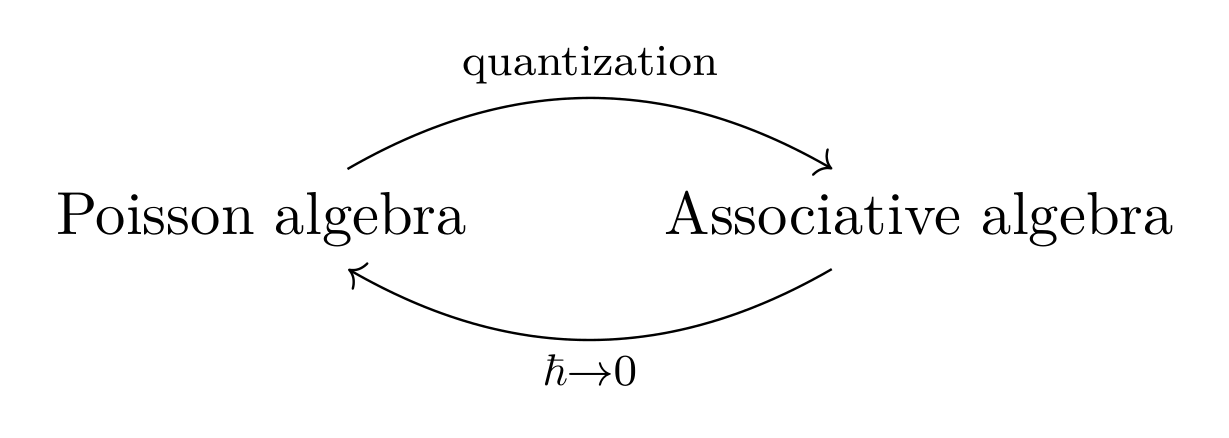
\includegraphics[width=0.49\linewidth]{fig_p077_1.png}
  \caption*{Poisson 代数与结合代数之间的量子化示意图（原文 PDF p.77 示意图，原文无编号）}
\end{figure}

% [Tutor Note: 上图是“量子化 = 结合代数结构的形变”这一图景的示意图：横向的
% “quantization”把 Poisson 代数变成结合代数，反向的“$\hbar\to0$”是经典极限
% （取 Poisson 括号为一阶项）。注意这里并没有说量子化函子是唯一的——形变量子化
% 的“唯一性/模空间”正是 9.3 节中特征类 $\omega_\hbar$ 所刻画的内容。]

这本质上就是量子力学中的量子化方法：经典相空间上的函数 $f$ 被量子化为算子 $\hat{f}$。

\begin{wdefn}{9.1}
  \emph{Poisson 流形}（Poisson manifold）是指一对 $(X,P)$，其中 $X$ 是光滑流形，
  $P\in\Gamma(X,\wedge^{2}TX)$ 且满足
  \[
    \{P,P\}_{SN}=0.
  \]
\end{wdefn}

这里 $\{-,-\}_{SN}$ 是 \emph{Schouten--Nijenhuis 括号}。$P$ 称为
\emph{Poisson 张量/双向量}。在局部坐标下可写为
\[
  P=\sum_{i,j}P^{ij}(x)\partial_i\wedge\partial_j.
\]
它在 $C^{\infty}(X)$ 上定义一个 \emph{Poisson 括号} $\{-,-\}_{P}$：
\[
  \{f,g\}_{P}:=\sum_{i,j}P^{ij}\partial_i f\partial_j g,
  \qquad \forall f,g\in C^{\infty}(X).
\]
此处 $\{P,P\}_{SN}=0$ 蕴涵 $\{-,-\}_{P}$ 满足 Jacobi 恒等式。因此 $\{-,-\}_{P}$
自然地定义了 Poisson 代数 $(C^{\infty}(X),\{-,-\}_{P})$。

% [Tutor Note: 此处极易出现 $1/2$ 因子的符号错误。定义 9.1 中
% $P=\sum_{i,j}P^{ij}\partial_i\wedge\partial_j$ 的求和\emph{不}带 $1/2$
% （$i,j$ 各自独立遍历，$i\neq j$ 的项被算了两次），故对应的括号公式
% $\{f,g\}_P=\sum_{i,j}P^{ij}\partial_i f\partial_j g$ 也\emph{不}带 $1/2$。
% 但例 9.2 中 $P=\omega^{-1}=\frac12\sum_{i,j}\omega^{ij}\partial_i\wedge\partial_j$
% 却显式写出 $1/2$：这是因为 $\omega^{ij}$ 按 $\omega=\frac12\sum\omega_{ij}
% \dd x^i\wedge\dd x^j$ 的约定取逆。核对任何文献时，先确认其
% $P^{ij}$ 的定义里是否含 $1/2$，再决定括号公式是否带 $1/2$。]

\begin{wexam}{9.2}
  设 $(X,\omega)$ 是辛流形，其中
  \[
    \omega=\frac12\sum_{i,j}\omega_{ij}\dd x^{i}\wedge\dd x^{j}
  \]
  是辛 $2$-形式。令
  \[
    P=\omega^{-1}=\frac12\sum_{i,j}\omega^{ij}\partial_i\wedge\partial_j,
  \]
  其中 $(\omega^{ij})$ 是 $(\omega_{ij})$ 的逆矩阵。则
  \[
    \dd\omega=0\iff\{P,P\}_{SN}=0.
  \]
  因此 $(X,\omega^{-1})$ 定义一个 Poisson 流形。
\end{wexam}

% >>> p078
\begin{wdefn}{9.3}
  Poisson 流形 $(X,P)$ 上的\emph{星积}（star-product）是一个 $\R[[\hbar]]$-双线性映射
  \[
    \begin{aligned}
      C^{\infty}(X)[[\hbar]]\times C^{\infty}(X)[[\hbar]]
        &\longrightarrow C^{\infty}(X)[[\hbar]],\\
      f\times g
        &\longmapsto f\star g=\sum_{k\ge0}\hbar^{k}c_k(f,g),
    \end{aligned}
  \]
  使得
  \begin{enumerate}[label=(\arabic*),leftmargin=2.2em,itemsep=0.2em]
    \item $\star$ 是结合的：$(f\star g)\star h=f\star(g\star h)$；
    \item $f\star g=fg+\mathcal{O}(\hbar)$，$\forall f,g\in C^{\infty}(X)$；
    \item $\frac12(f\star g-g\star f)=\hbar\{f,g\}+\mathcal{O}(\hbar^{2})$，
          $\forall f,g\in C^{\infty}(X)$；
    \item $c_k:C^{\infty}(X)\times C^{\infty}(X)\to C^{\infty}(X)$ 是双微分算子。
  \end{enumerate}
  此时称 $(C^{\infty}(X)[[\hbar]],\star)$ 为 $(X,P)$ 的\emph{形变量子化}
  （deformation quantization）。
\end{wdefn}

% [Tutor Note: 星积公理 (3) 的系数是关键：$\frac12(f\star g-g\star f)$ 的一阶项
% 必须等于 $\hbar\{f,g\}$，故 $c_1$ 的反对称部分就是 Poisson 括号；换言之
% $c_1(f,g)=\frac12\{f,g\}+$（某个对称双微分算子）。物理文献中常用的 Moyal 积
% 是指数里带 $\ii\hbar/2$ 的版本（见下例的约定），与本节的 $\hbar$ 实系数版本
% 只差 $\hbar\to\ii\hbar$ 及符号，跨文献搬运公式时务必先核对这一处。
% 另注：原文在 p.76–77（PDF p.77–78）若干处把 $C^{\infty}(X)$ 印成
% $C^{\infty}(x)$（小写 $x$，如定义 9.1 之后与定义 9.3 中）；本译本按全书记号
% 统一为 $C^{\infty}(X)$，特此说明。]

形变量子化的定义是纯代数的。形变量子化的\emph{存在性}却极不平凡。
DeWilde--Lecomte \textup{[13]} 于 1983 年用上同调方法得到了辛流形上形变量子化的
一般存在性。独立地，Fedosov \textup{[17]} 于 1985 年用微分几何方法给出了另一条
漂亮的进路。更一般地，Kontsevich \textup{[26]} 对一般 Poisson 流形给出了完全解答。

\begin{wexam}{9.4}
  设 $X=\R^{2n}$，Poisson 张量为
  \[
    P=\frac12\sum_{i,j}P^{ij}\partial_i\wedge\partial_j.
  \]
  这里 $P^{ij}$ 为常数。给定 $f(x),g(x)$，如下定义 \emph{Moyal 积} $\star$：
  \[
    (f\star g)(x)
      =\exp\left(\frac{\hbar}{2}\sum_{i,j}P^{ij}
        \frac{\partial}{\partial y^{i}}\frac{\partial}{\partial z^{j}}\right)
      \Big|_{y=z=x}f(y)g(z),
  \]
  或用图形表示，
  \begin{figure}[htbp]
  \centering
  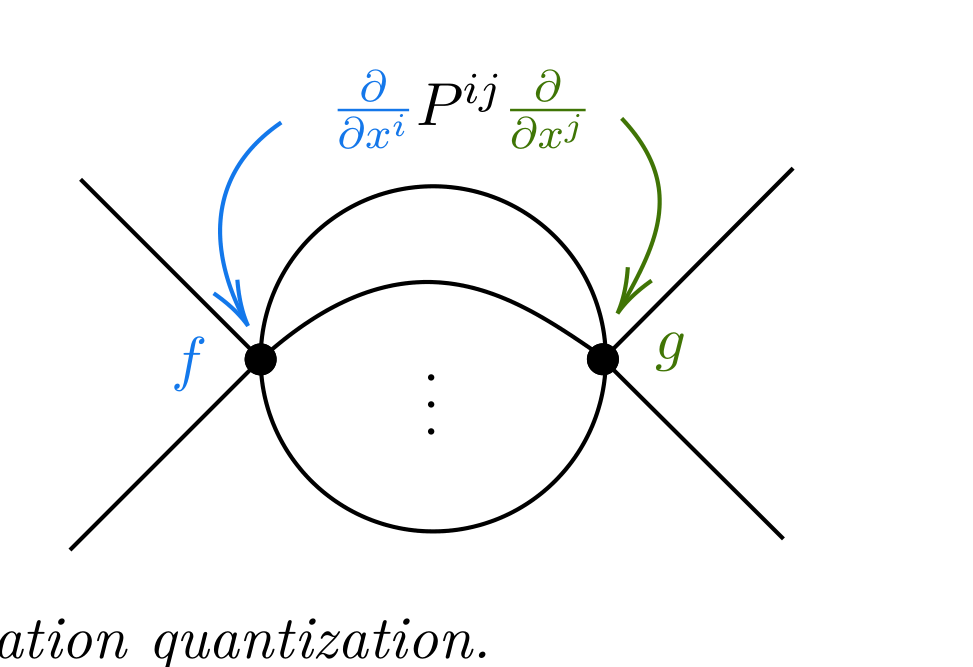
\includegraphics[width=0.39\linewidth]{fig_p078_1.png}
  \caption*{Moyal 积的图形表示（原文 PDF p.78 示意图，原文无编号）}
\end{figure}
  则 $\star$ 定义一个形变量子化。
\end{wexam}

\begin{wrem}{9.5}
  若 $P^{ij}\neq$ 常数，则上述公式不再适用。
\end{wrem}

BV 结构自然地如下出现。设 $(V,\omega)$ 是线性辛空间，其中 $V\simeq\R^{2n}$，
$\omega:\wedge^{2}V\to\R$ 是辛配对。记
\[
  \widehat{\mathcal{O}}(V):=\widehat{\operatorname{Sym}}(V^{\vee})
  =\prod_{k\ge0}\operatorname{Sym}^{k}(V^{\vee}),
\]
其中 $V^{\vee}=\Hom(V,\R)$ 是 $V$ 的线性对偶。于是 Moyal--Weyl 积定义一个结合代数
$\big(\widehat{\mathcal{O}}(V)[[\hbar]],\star\big)$，称为（形式）Weyl 代数。

% [Tutor Note: Moyal 公式（例 9.4）中指数上必须同时含 $\partial/\partial y^i$ 与
% $\partial/\partial z^j$，而 $P^{ij}$ 夹在中间；最后在 $y=z=x$ 处取值。
% 系数 $\hbar/2$ 与 $P^{ij}$ 的归一化直接相关（见定义 9.1 的批注）。
% 若 $P^{ij}$ 非常数，该指数公式失效——因为此时导数与 $P^{ij}(x)$ 不再交换，
% 必须改用 Fedosov 或 Kontsevich 的构造（见注 9.5）。
% 又，此处 $\widehat{\operatorname{Sym}}(V^\vee)=\prod_{k\ge0}
% \operatorname{Sym}^k(V^\vee)$ 用的是\emph{直积}（形式幂级数）而非直和
% （多项式）：Weyl 代数要容纳无穷阶形式幂级数，这是 $\hbar$-进完备化的需要。
% 这一“直积 vs 直和”的区别在定义 9.6 的 Weyl 丛中同样出现，若误写成
% $\oplus$ 则得到的是多项式系数的 Weyl 代数，不能刻画 Fedosov 联络的完备性。]

% >>> p079
\subsection{Fedosov 量子化（Fedosov Quantization）}

现在我们聚焦于辛流形。Fedosov \textup{[17]} 对辛情形给出了形变量子化的一个简单而
几何的构造。在辛流形 $(X,\omega)$ 上，每一点 $p\in X$ 处的切平面 $T_pX$ 是线性辛空间。
量子涨落把 $T_pX$ 上函数代数形变为相应的 Weyl 代数。这些逐点的 Weyl 代数构成一个
向量丛——$X$ 上的 \emph{Weyl 丛} $\mathcal{W}(X)$。

\begin{wdefn}{9.6}
  设 $(X,\omega)$ 是辛流形。定义 \emph{Weyl 丛}
  \[
    \mathcal{W}(X):=\prod_{k\ge0}\operatorname{Sym}^{k}(T^{*}X)[[\hbar]].
  \]
  于是在每一点 $p\in X$ 处，其纤维为
  \[
    \mathcal{W}(X)\big|_{p}=\widehat{\mathcal{O}}(T_pX)[[\hbar]].
  \]
  这里 $\widehat{\mathcal{O}}$ 指形式幂级数函数。
\end{wdefn}

$\mathcal{W}(X)$ 的一个局部截面为
\[
  \sigma(x,y)=\sum_{k,l\ge0}\hbar^{k}a_{k,i_1\cdots i_l}(x)
  y^{i_1}\cdots y^{i_l},
\]
其中 $\{x\}$ 是底流形坐标、$\{y\}$ 是纤维坐标，$a_{k,i_1\cdots i_l}(x)$ 是光滑函数。
由于 $\big(T_pX,\omega|_{T_pX}\big)$ 是线性辛空间，我们有逐纤维的 Moyal 积，仍记作
$\star$。于是 $(\mathcal{W}(X),\star)$ 定义了一个无穷维的代数丛。

设 $\nabla$ 是 $TX$ 上的一个无挠且与 $\omega$ 相容（即 $\nabla\omega=0$）的联络。
这样的联络称为\emph{辛联络}（symplectic connection；它总是存在，且不唯一）。
$\nabla$ 诱导出所有张量丛上的联络，特别地，它定义了 $\mathcal{W}(X)$ 上的一个联络，
仍记作 $\nabla$。其曲率为
\[
  \nabla^{2}\sigma=\frac{1}{\hbar}[R_{\nabla},\sigma]_{\star},
  \qquad \forall\sigma\in\Gamma(X,\mathcal{W}(X)),
\]
其中
\[
  R_{\nabla}=\frac14 R_{ijkl}y^{i}y^{j}\dd x^{k}\wedge\dd x^{l}
  \in\Omega^{2}(X,\mathcal{W}(X))
\]
是取值于 Weyl 丛 $\mathcal{W}(X)$ 的 $2$-形式；$R_{ijkl}=\omega_{im}R^{m}{}_{jkl}$ 是
与辛配对缩并后的曲率形式。

给定 $X$ 上一列闭 $2$-形式 $\{\omega_k\}_{k\ge1}$，Fedosov 证明了：在相差规范变换的
意义下，存在唯一的 $\mathcal{W}(X)$ 上形如 $\nabla+\frac{1}{\hbar}[\gamma,-]_{\star}$
的联络，其中 $\gamma\in\Omega^{1}(X,\mathcal{W}(X))$ 是取值于 $\mathcal{W}(X)$ 的
$1$-形式，它满足某些初始条件以及 \emph{Fedosov 方程}
\[
  \nabla\gamma+\frac{1}{2\hbar}[\gamma,\gamma]_{\star}+R_{\nabla}=\omega_{\hbar},
\]
其中 $\omega_{\hbar}=-\omega+\sum_{k\ge1}\hbar^{k}\omega_k$。令
\[
  D=\nabla+\frac{1}{\hbar}[\gamma,-]_{\star}
\]
为 \emph{Fedosov 联络}。于是 Fedosov 方程蕴涵
\[
  D^{2}=\frac{1}{\hbar}[\omega_{\hbar},-]_{\star}=0.
\]

% >>> p080
其中 $\omega_{\hbar}$ 沿每个纤维为常数，因而是一个中心项。于是我们得到
$\mathcal{W}(X)$ 上的平坦联络 $D$。后面将会看到，Fedosov 联络具有\emph{量子主方程}
的几何解释 \textup{[21, 24]}。

令 $\mathcal{W}_{D}(X):=\{\sigma\in\Gamma(X,\mathcal{W}(X))\mid D\sigma=0\}$ 为平坦
截面的空间。则 $(\mathcal{W}_{D}(X),\star)$ 是一个结合代数。设
\[
  \sigma:\ \mathcal{W}_{D}(X)\longrightarrow C^{\infty}(X)[[\hbar]]
\]
为把 $y\mapsto0$ 的\emph{符号映射}（symbol map）。则 $\sigma$ 是同构，且
\[
  f\star g\mapsto\sigma\big(\sigma^{-1}(f)\star\sigma^{-1}(g)\big)
\]
定义一个形变量子化。$\omega_{\hbar}$ 就是相应的\emph{特征类}（或模）。

% [Tutor Note: Fedosov 方程（p.79 页脚 / PDF p.79）是本章最核心也最容易抄错的公式。
% 三点提醒：(i) 第二项系数是 $1/(2\hbar)$ 而非 $1/\hbar$，来自 $\gamma$ 的二次项；
% (ii) $\omega_\hbar=-\omega+\sum_{k\ge1}\hbar^k\omega_k$ 中的负号是必需的——
% 它与 $\nabla$ 的无挠辛性一起保证 $D^2$ 只用 $\omega_\hbar$ 的中心项表达；
% (iii) 不同文献对 $R_\nabla$ 的符号（以及 $\omega_\hbar$ 中 $-\omega$ 还是 $+\omega$）
% 有不同约定，恰好相差整体符号；比对时以 $D^2=0$ 与 $[\omega_\hbar,-]_\star$ 的
% 中心性为锚点。
% 又，符号映射 $\sigma$（把 $y\mapsto0$）在这里被用来“搬运”星积：平坦截面代数
% $(\mathcal{W}_D(X),\star)$ 与函数代数 $C^\infty(X)[[\hbar]]$ 通过 $\sigma$ 同构，
% 于是 $f\star g:=\sigma(\sigma^{-1}(f)\star\sigma^{-1}(g))$。注意 $\sigma$ 同时是
% 记号（映射名）与 Weyl 丛截面的记号，原文混用；阅读公式时须由上下文区分。
% 特征类 $\omega_\hbar$ 的选取对应不同的形变量子化，这正是“模”的含义。]

\subsection{代数指标定理（Algebraic Index Theorem）}

给定辛流形上带特征类 $\omega_{\hbar}$ 的形变量子化
$(C^{\infty}(X)[[\hbar]],\star)$，存在唯一的\emph{迹映射}（trace map）
\[
  \Tr:\ C^{\infty}(X)[[\hbar]]\longrightarrow\R((\hbar))
\]
满足一个归一化条件以及迹性质：
\[
  \Tr(f\star g)=\Tr(g\star f).
\]
于是指标作为该理论的配分函数得到，可表述为
\[
  \operatorname{Index}=\Tr(1)=\int_{X}\ee^{\omega_{\hbar}/\hbar}\widehat{A}(X),
\]
其中 $\widehat{A}(X)$ 是 $X$ 的（形式）$\widehat{A}$ 类。这是由 Fedosov \textup{[18]}
与 Nest--Tsygan \textup{[37]} 作为 Atiyah--Singer 指标定理的代数类比而表述的
\emph{代数指标定理}的最简单版本。

% [Tutor Note: $\widehat{A}$ 类（Â 类）是 Pontryagin 形式的通用级数
% $\widehat{A}(X)=\det^{1/2}\big(\tfrac{R/2}{\sinh(R/2)}\big)$（$R$ 为曲率
% $2$-形式矩阵），在此作为形式幂级数处理。$\ee^{\omega_\hbar/\hbar}$ 的
% $\hbar^{-n}$ 项就是 $\frac{(-1)^n}{n!}\omega^n\hbar^{-n}$，给出辛体积
% （$2n=\dim X$）；其余各项按 $\hbar$ 幂次（含 $\hbar^0$ 项）给出由曲率形式
% 组合成的拓扑指标——这正是与 Atiyah--Singer 指标定理对应的部分
% （不同文献对 $\omega_k$ 的归一化相差常数，比较时逐项核对 $\hbar$ 幂次）。
% 带 $\operatorname{Ch}(E)$ 的版本见下式。]

我们也可以类似地为 $C^{\infty}(X,\operatorname{End}(E))[[\hbar]]$ 构造形变量子化并
构造迹映射，于是得到
\[
  \Tr(1)=\int_{X}\ee^{\omega_{\hbar}/\hbar}\operatorname{Ch}(E)\widehat{A}(X),
\]
其中 $\operatorname{Ch}(E)$ 是 $X$ 上向量丛 $E$ 的 Chern 特征。

\paragraph{与 QFT 的关系（Relation with QFT）}

在超对称（SUSY）量子场论中，\emph{局部化}（localization）经常出现：场空间
$\mathcal{E}$ 上的路径积分往往被有效地局部化为有限维空间 $M\subset\mathcal{E}$ 上
的等价积分，而 $M$ 描述某个有趣的模空间：
\[
  \int_{\mathcal{E}}\ee^{\ii S/\hbar}=\int_{M}(-).
\]
在拓扑量子力学中，我们发现
\[
  \int_{\operatorname{Map}(S^{1},X)}\ee^{-S/\hbar}
  \ \overset{\hbar\to0}{=}\
  \int_{X}(-),
\]

% [Tutor Note: 这两个积分的“$(-)$”表示被积的恰当对象（在 $M$ 或 $X$ 上待定的
% 形式），重点是\emph{积分区域}的局部化，而非被积函数的具体形式。
% $\overset{\hbar\to0}{=}$ 表示在 $\hbar\to0$ 的精确半经典近似下等式成立：
% 路径积分被常数映射附近的形式邻域上的有效理论完全捕获，因而化归为 $X$ 上的
% 有限维积分。左侧通常给出某椭圆算子解析指标的物理表述，右侧则给出由各种曲率
% 形式组合而成的拓扑指标。]

% >>> p081
其中 $\operatorname{Map}(S^{1},X)$ 是回路空间，$\int_{X}$ 表示局部化到\emph{常值
映射}。路径积分将被常数映射在完整映射空间内的形式邻域上的有效理论精确捕获。
$\hbar\to0$ 下的精确半经典近似使我们能把路径积分约化为常值映射模空间（即 $X$）上
一个有意义的积分。左端通常给出某个椭圆算子解析指标的物理表述；右端最终会写成
各种曲率形式的积分，代表拓扑指标。

\begin{figure}[htbp]
  \centering
  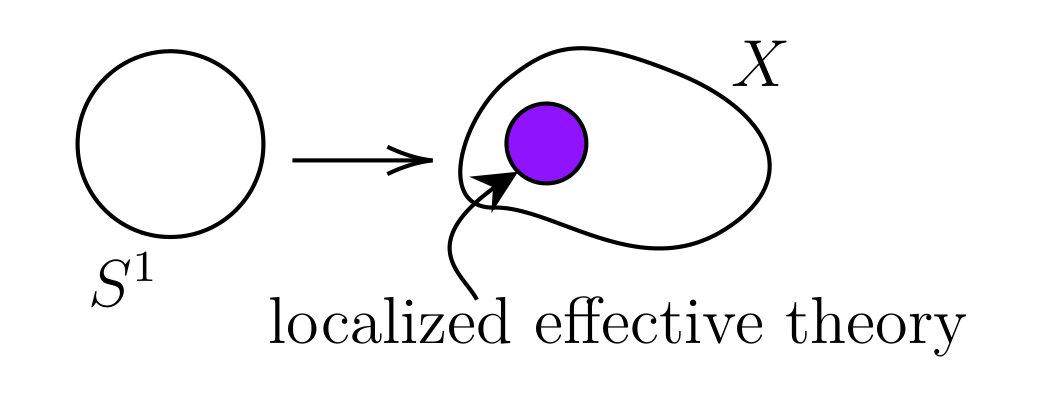
\includegraphics[width=0.42\linewidth]{fig_p081_1.png}
  \caption*{回路空间局部化到 $X$ 中一点的邻域（左图）（原文 PDF p.81 示意图，原文无编号）}
\end{figure}

\begin{figure}[htbp]
  \centering
  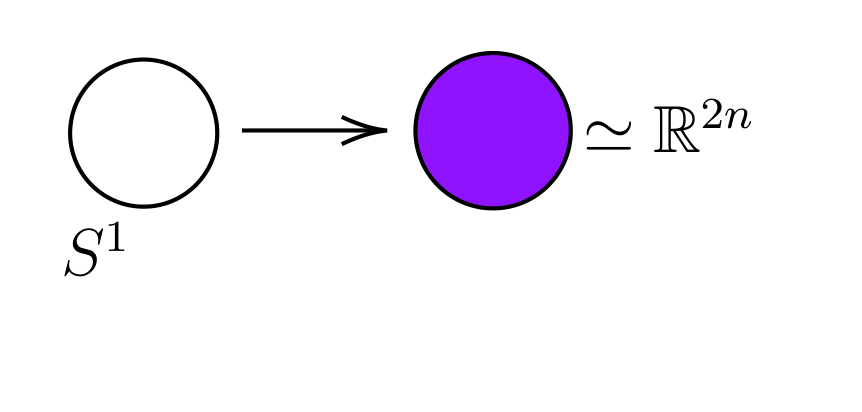
\includegraphics[width=0.35\linewidth]{fig_p081_2.png}
  \caption*{局部化到 $\R^{2n}$ 的标准相空间（右图）（原文 PDF p.81 示意图，原文无编号）}
\end{figure}

几何上，回路空间被映到 $X$ 中某点（由常值映射指定）的局部化邻域，该邻域上存在
一个局部化的有效理论。局部地，通过选取 Darboux 坐标，$X$ 可以看作标准相空间
$\R^{2n}$。于是回路空间在 $X$ 上粘接成一族有效场论。这可以在有效 BV 量子化
\textup{[24]} 的框架内严格地完成：
\begin{itemize}[leftmargin=1.8em,itemsep=0.25em]
  \item 有效作用量 $\leadsto\gamma$；
  \item 量子主方程（QME）$\leadsto$ Fedosov 方程；
  \item BV 积分 $\leadsto$ 迹映射；
  \item 配分函数 $\leadsto$ 代数指标。
\end{itemize}

\subsection{局部理论（Local Theory）}

本节我们用有效重整化方法研究拓扑量子力学，并用它证明代数指标定理。我们遵循
\textup{[21, 24]} 中的表述。

\paragraph{局部模型（Local Model）}

考虑标准相空间 $(V,\omega)$，其中 $V\simeq\R^{2n}$，坐标为
\[
  (x^{1},\cdots,x^{n},x^{n+1},\cdots,x^{2n})
  =(q^{1},\cdots,q^{n},p_1,\cdots,p_n),
\]
并且
\[
  \omega=\sum_{i=1}^{n}\dd p_i\wedge\dd q^{i}.
\]
设 $S^{1}_{dR}$ 是这样的（局部环）空间：其底拓扑空间是圆周 $S^{1}$，结构层为
$\mathcal{O}(S^{1}_{dR})=\Omega^{\bullet}_{S^{1}}$，这是一个由微分形式构成的 dg
（微分分次）环，其微分是 de Rham 微分算子 $\dd$。

考虑描述映射空间
\[
  \varphi:\ S^{1}_{dR}\longrightarrow V\simeq\R^{2n}
\]
的\emph{局部模型}。这样的 $\varphi$ 可以等同于 $\Omega^{\bullet}_{S^{1}}\otimes V$
中的一个元素。具体地说，设 $\theta$ 是 $S^{1}$ 上的坐标（带有等同
$\theta\sim\theta+1$）。映射空间于是可写为
\[
  \{\varphi\}=\big\{\mathbb{P}_i(\theta),\mathbb{Q}^{i}(\theta)\big\}_{i=1,\cdots,n},
  \qquad \mathbb{P}_i,\mathbb{Q}^{i}\in\Omega^{\bullet}_{S^{1}}.
\]

% [Tutor Note: $S^{1}_{dR}$ 是“以圆周为底拓扑、以 de Rham 复形为结构层”的
% dg 流形（局部环空间），因此到 $\R^{2n}$ 的“映射”不是普通连续映射，而是
% $\Omega^{\bullet}_{S^{1}}\otimes V$ 中的元素——即取值于 $V$ 的微分形式。
% 这正是 BV 形式中“场 = 形式次数可变的量”的来源：$\mathbb{P}_i,\mathbb{Q}^i$
% 可以是 $0$-形式（$p_i,q^i$）也可以是 $1$-形式（$\eta_i,\xi^i$）。
% 记 $\Omega^{\bullet}_{S^1}$ 的 $\bullet$ 为形式次数，勿与上同调次数混淆。]

% >>> p082
写成分量形式，
\[
  \mathbb{P}_i(\theta)=p_i(\theta)+\eta_i(\theta)\dd\theta,
  \qquad
  \mathbb{Q}^{i}(\theta)=q^{i}(\theta)+\xi^{i}(\theta)\dd\theta.
\]
于是场空间为
\[
  \mathcal{E}=\Omega^{\bullet}_{S^{1}}\otimes V.
\]
三元组
\[
  \Big(\Omega^{\bullet}_{S^{1}}\otimes V,\ \dd,\
  \int_{S^{1}}\langle-,-\rangle_{\omega}\Big)
\]
是一个无穷维的 $(-1)$-dg 辛空间。作用是自由作用量：
\[
  \begin{aligned}
    S[\varphi]
      &:=\int_{S^{1}}\langle\varphi,\dd\varphi\rangle_{\omega}\\
      &=\sum_i\int_{S^{1}}\mathbb{P}_i\dd\mathbb{Q}^{i}
      =\sum_i\int_{S^{1}}p_i(\theta)\dd q^{i}(\theta).
  \end{aligned}
\]

\begin{wrem}{9.7}
  这是沿 AKSZ 构造 \textup{[1]} 的拓扑量子力学的一阶形式（first-order formalism）。
\end{wrem}

\paragraph{传播子（Propagator）}

我们选取 $S^{1}$ 上的标准平坦度量。设 $\dd^{*}$ 是 $\dd$ 的伴随算子。Laplacian 为
\[
  [\dd,\dd^{*}]=-\left(\frac{\dd}{\dd\theta}\right)^{2}.
\]
令
\[
  \Pi=\omega^{-1}
  =\sum_i\frac{\partial}{\partial p_i}\wedge\frac{\partial}{\partial q^{i}}
  =\frac12\sum_i\left(
    \frac{\partial}{\partial p_i}\otimes\frac{\partial}{\partial q^{i}}
    -\frac{\partial}{\partial q^{i}}\otimes\frac{\partial}{\partial p_i}
  \right)\in\wedge^{2}V
\]
为 \emph{Poisson 双向量}（或 Poisson 核）。令
\[
  h_t(\theta_1,\theta_2)=\frac{1}{\sqrt{4\pi t}}
  \sum_{n\in\Z}\ee^{-\frac{(\theta_1-\theta_2+n)^{2}}{4t}}
\]
为 $S^{1}$ 上的标准热核。于是正则化传播子为
\[
  P^{L}_{\varepsilon}=\int_{\varepsilon}^{L}
  \partial_{\theta_1}h_t(\theta_1,\theta_2)\dd t\otimes\Pi
  \in\mathcal{E}\otimes\mathcal{E},
\]
其中 $\int_{\varepsilon}^{L}\partial_{\theta_1}h_t(\theta_1,\theta_2)\dd t
\in C^{\infty}(S^{1}\times S^{1})$ 且 $\Pi\in V\otimes V$。记
\[
  P^{S^{1}}(\theta_1,\theta_2)
  =\int_{0}^{\infty}\partial_{\theta_1}h_t(\theta_1,\theta_2)\dd t.
\]
则完整传播子由
\[
  P^{\infty}_{0}=P^{S^{1}}\otimes\Pi
\]
给出。

% [Tutor Note: 传播子的构造有三处易错：(i) 被积的是 $\partial_{\theta_1}h_t$（对
% 第一个变量的导数），不是 $\partial_t h_t$，也不是 $h_t$ 本身；(ii) $\varepsilon$
% 是 UV 截断（$t$ 的下限），$L$ 是标度，取 $\varepsilon\to0$、$L\to\infty$ 得到
% 完整传播子；(iii) $\Pi\in\wedge^2V\subset V\otimes V$，其 $\frac12$ 系数与定义 9.1
% 中 Poisson 张量的约定一致——若漏掉 $\frac12$，$P^\infty_0$ 会差一个因子 2。
% 又，$[\dd,\dd^*]=-(\dd/\dd\theta)^2$ 的符号取决于 $1$-形式的伴随定义
% （$\int\alpha\wedge*\beta$ 的约定）；这里取平坦度量使 $\dd^*=-\partial_\theta$
% 在 $1$-形式上。该式说明 Laplacian 在 $0$-形式与 $1$-形式上分别作用为
% $-\partial_\theta^2$，是热核 $h_t$ 满足热方程的依据。]

\begin{wprop}{9.8}
  $P^{S^{1}}(\theta_1,\theta_2)$ 是 $\theta_1-\theta_2\in\R/\Z$ 的如下周期函数：
  当 $0<\theta_1-\theta_2<1$ 时，
  \[
    P^{S^{1}}(\theta_1,\theta_2)=\theta_1-\theta_2-\frac12.
  \]
\end{wprop}

% >>> p083
\begin{figure}[htbp]
  \centering
  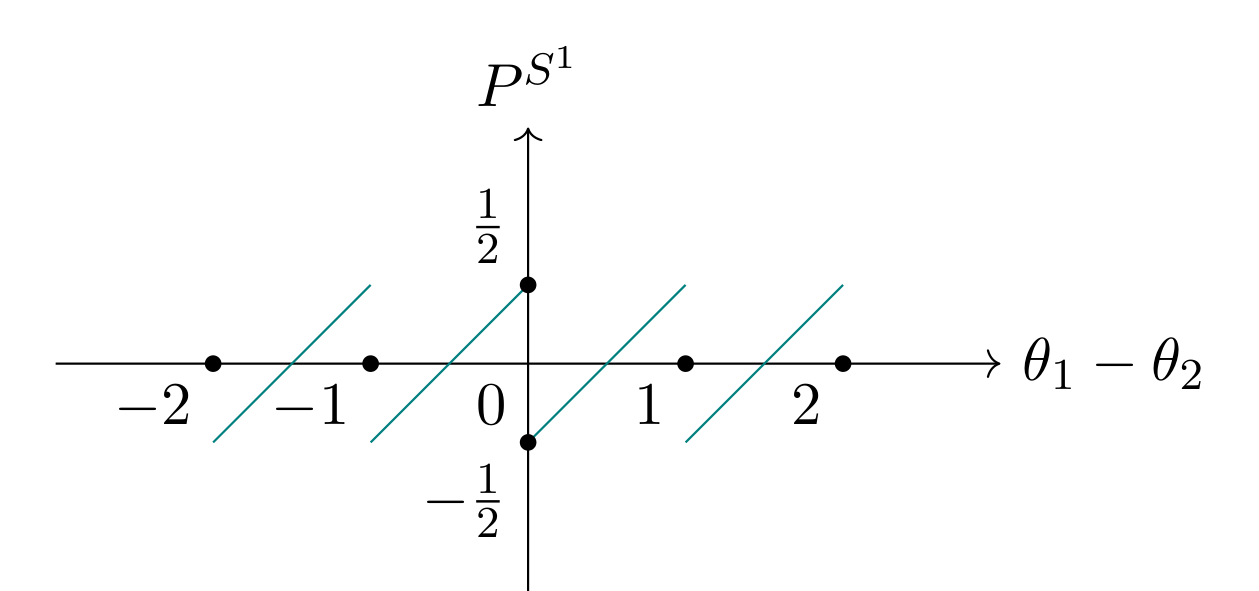
\includegraphics[width=0.51\linewidth]{fig_p083_1.png}
  \caption*{$P^{S^1}$ 作为 $\theta_1-\theta_2$ 的周期函数的图像（原文 PDF p.83 示意图，原文无编号）}
\end{figure}

$P^{S^{1}}$ \emph{不是} $S^{1}\times S^{1}$ 上的光滑函数（正如所料），但它是有界的。

% [Tutor Note: 命题 9.8 的函数是 Bernoulli 多项式 $B_1$ 的周期化（锯齿波），
% 在整数点有跳跃，因此不是 $S^1\times S^1$（紧流形）上的光滑函数——这正是
% 拓扑量子力学作为“拓扑”理论却仍有非平凡传播子的原因：它在 $L^\infty$ 意义下
% 有界，故 $\exp(\hbar P^\infty_0)$ 作为形式幂级数是良定义的（见下方 HRG 流）。
% 平移常数 $-\frac12$ 与“哪个变量取导数”“热核归一化”的约定有关，换文献时
% 可能变为 $+\frac12$，但锯齿波形状与有界性不变。]

\paragraph{关联映射（Correlation Map）}

记形式 Weyl 代数
\[
  \mathcal{W}_{2n}=\big(\R[[p_i,q^{i}]]((\hbar)),\star\big),
\]
以及形式 Weyl 子代数
\[
  \mathcal{W}^{+}_{2n}=\big(\R[[p_i,q^{i}]][[\hbar]],\star\big),
\]
其中 $\star$ 是 Moyal--Weyl 积。我们可以把形式 Weyl 子代数等同于 $V$ 上的（形式）
函数（经由形变量子化）：
\[
  \mathcal{W}^{+}_{2n}\simeq\big(\widehat{\mathcal{O}}(V)[[\hbar]],\star\big).
\]

给定 $f_0,f_1,\cdots,f_m\in\mathcal{W}_{2n}$，如下定义
$\mathcal{O}_{f_0,f_1,\cdots,f_m}\in\mathcal{O}(\mathcal{E})((\hbar))$：
\[
  \mathcal{O}_{f_0,f_1,\cdots,f_m}[\varphi]
  :=\int_{0<\theta_1<\theta_2<\cdots<\theta_m<1}
  \dd\theta_1\dd\theta_2\cdots\dd\theta_m\,
  f^{(0)}_{0}\big(\varphi(\theta_0)\big)
  f^{(1)}_{1}\big(\varphi(\theta_1)\big)\cdots
  f^{(1)}_{m}\big(\varphi(\theta_m)\big).
\]
这里 $\varphi\in\Omega^{\bullet}_{S^{1}}\otimes V$。令
$f(\varphi(\theta))=f(\mathbb{P}_i(\theta),\mathbb{Q}^{i}(\theta))
\in\Omega^{\bullet}_{S^{1}}$，并把它分解为
\[
  f(\varphi(\theta))=f^{(0)}(\varphi(\theta))
  +f^{(1)}(\varphi(\theta))\dd\theta.
\]

\begin{figure}[htbp]
  \centering
  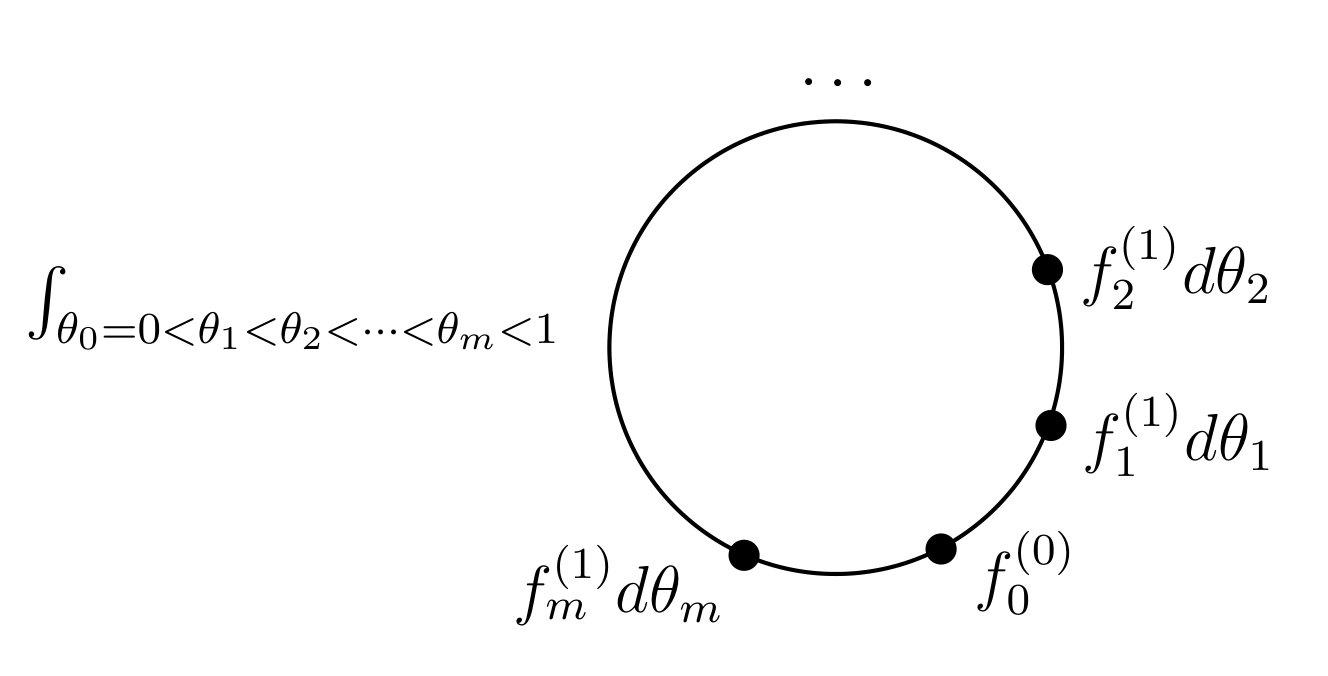
\includegraphics[width=0.53\linewidth]{fig_p083_2.png}
  \caption*{可观测量 $\mathcal{O}_{f_0,\dots,f_m}$ 的圆周插入表示（原文 PDF p.83 示意图，原文无编号）}
\end{figure}

\begin{wrem}{9.9}
  $f^{(1)}(\varphi)$ 是 $f^{(0)}(\varphi)$ 在 Witten 意义下的\emph{拓扑下降}
  （topological descent）。
\end{wrem}

% [Tutor Note: 插入次序 $0<\theta_1<\cdots<\theta_m<1$ 是定义的一部分，不能随意
% 交换：交换两个插入点会因 $f^{(1)}$ 中含 $\dd\theta$（奇元素）而带来符号改变。
% 这就是“因子化乘积”在拓扑量子力学中表现为按圆周次序排列的积分的原因；
% $f^{(0)}$ 放在 $\theta_0=0$ 处，其余 $f^{(1)}\dd\theta_i$ 依次插入。
% “拓扑下降”指出：$\dd(f^{(0)}(\varphi))=f^{(1)}(\varphi)\dd\theta$ 之类关系
% 把 $0$-形式可观测量与 $1$-形式可观测量联系起来，这正是 $B$ 算子与
% de Rham 微分 $d_{2n}$ 相对应的物理来源。]

现在我们对 $\exp(\hbar P^{\infty}_{0})\big(\mathcal{O}_{f_0,f_1,\cdots,f_m}\big)$
施加 HRG 流。由于 $P^{\infty}_{0}$ 有界，它是收敛的、良定义的！这就是\emph{UV 有限}
性质。

如我们已经讨论过的，在 $L=\infty$ 处，可以把它看作定义零模上的函数：
\[
  \HH=H^{\bullet}\big(\Omega^{\bullet}_{S^{1}}\otimes V,\dd\big)
  =H^{\bullet}(S^{1})\otimes V=V\oplus V\dd\theta.
\]
我们有 $\widehat{\mathcal{O}}(\HH)=\widehat{\Omega}^{\bullet}_{2n}$，即 $V$ 上的形式。

% >>> p084
\begin{wdefn}{9.10}
  如下定义\emph{关联映射}（correlation map）：
  \[
    \langle\cdots\rangle_{free}:\
    \mathcal{W}_{2n}\otimes\cdots\otimes\mathcal{W}_{2n}
    \longrightarrow\widehat{\Omega}^{\bullet}_{2n}((\hbar)),
  \]
  其定义为
  \[
    \langle f_0\otimes f_1\otimes\cdots\otimes f_m\rangle_{free}
    :=\exp(\hbar P^{\infty}_{0})
    \big(\mathcal{O}_{f_0,f_1,\cdots,f_m}\big)\big|_{\HH}.
  \]
\end{wdefn}

从路径积分的角度看，这就是
\[
  \langle f_0\otimes f_1\otimes\cdots\otimes f_m\rangle_{free}(\alpha)
  =\int_{\operatorname{Im}\dd^{*}\subset\mathcal{E}}[\mathcal{D}\varphi]\,
  \ee^{-S[\varphi+\alpha]/\hbar}
  \mathcal{O}_{f_0,f_1,\cdots,f_m}[\varphi+\alpha],
  \qquad \alpha\in\HH=H^{\bullet}(S^{1})\otimes V.
\]
这里零模 $\alpha$ 被看作背景场。它也可以如下用 Feynman 图表示。

\begin{figure}[htbp]
  \centering
  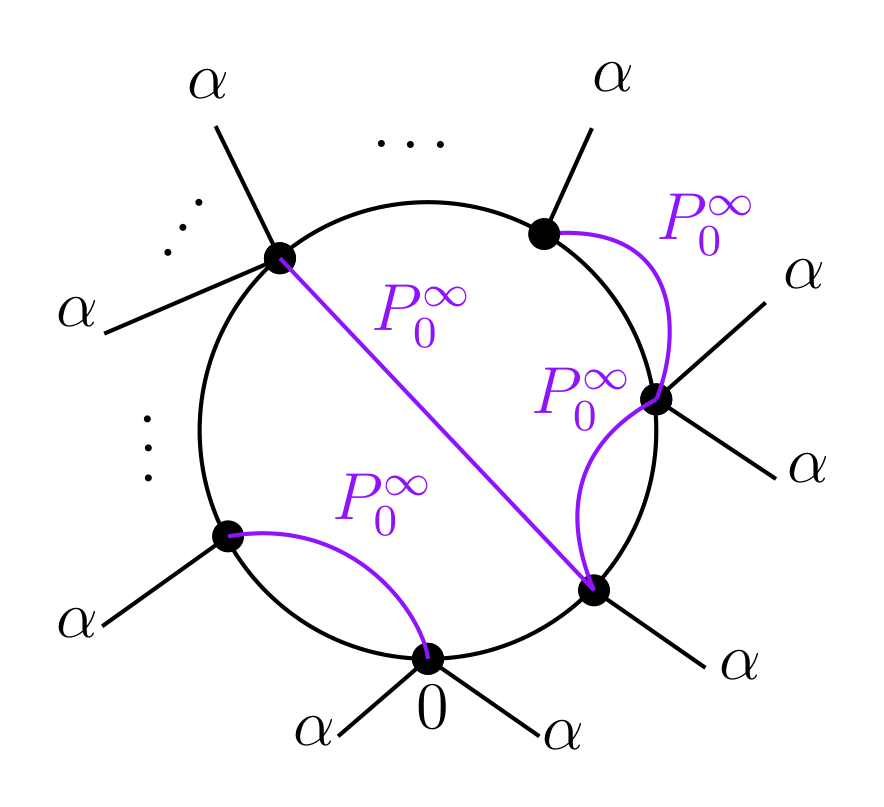
\includegraphics[width=0.35\linewidth]{fig_p084_1.png}
  \caption*{关联函数的 Feynman 图表示（原文 PDF p.84 示意图，原文无编号）}
\end{figure}

\paragraph{回顾（循环）Hochschild 复形（(Cyclic) Hochschild Complex Reviewed）}

设 $A$ 是含幺结合代数，$\overline{A}:=A/(\C\cdot1)$。令
$C_{-p}(A):=A\otimes\overline{A}^{\otimes p}$ 为循环 $p$-链。它带有自然的
\emph{Hochschild 微分}
\[
  b:\ C_{-p}(A)\longrightarrow C_{-p+1}(A),\qquad p\ge1,
\]
其定义为
\[
  b(a_0\otimes\cdots\otimes a_p)
  =(-1)^{p}a_pa_0\otimes\cdots\otimes a_{p-1}
  +\sum_{i=0}^{p-1}(-1)^{i}
  a_0\otimes\cdots\otimes a_ia_{i+1}\otimes\cdots\otimes a_p.
\]

\begin{figure}[htbp]
  \centering
  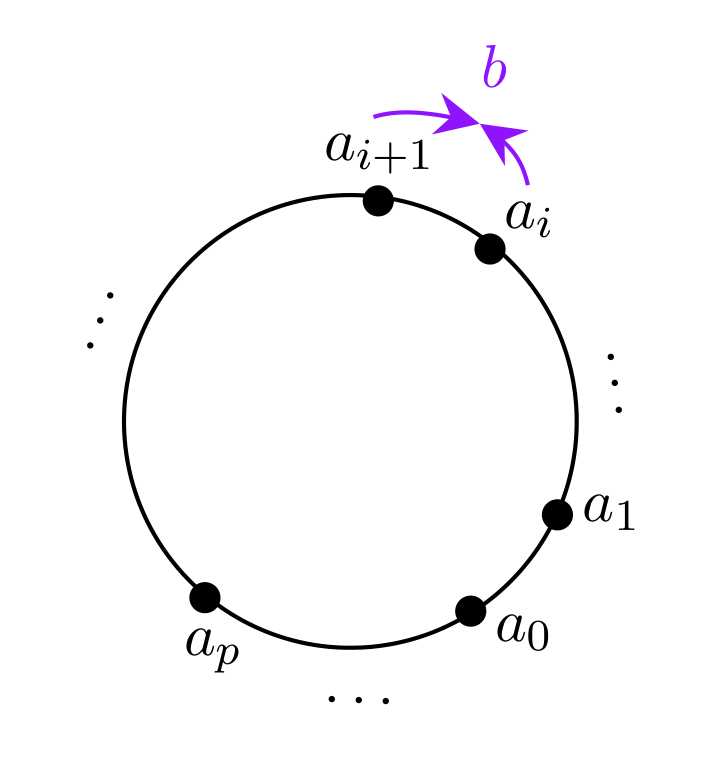
\includegraphics[width=0.28\linewidth]{fig_p084_2.png}
  \caption*{Hochschild 微分 $b$ 的圆周收缩图（原文 PDF p.84 示意图，原文无编号）}
\end{figure}

于是结合性蕴涵 $b\circ b=0$。因此，$(C_{-\bullet}(A),b)$ 定义了
\emph{Hochschild 链复形}。

% [Tutor Note: $b$ 的符号约定在文献中差异极大（有的把 $(-1)^p$ 换成
% $(-1)^{p+1}$，或把 $(-1)^i$ 换成 $(-1)^{i+1}$），但 $b^2=0$ 与
% “$b$ 是同伦意义的边界算子”这两点不变。原文用的是 $(-1)^pa_pa_0$ 与
% $(-1)^i$；抄写时务必逐符号对照，尤其不要把 $a_ia_{i+1}$（相邻两个相乘后
% 只占一个位置）写成 $a_i\otimes a_{i+1}$。]

我们还可以定义 \emph{Connes 算子}：
\[
  B:\ C_{-p}(A)\longrightarrow C_{-p-1}(A),
\]

% >>> p085
其定义为
\[
  B(a_0\otimes\cdots\otimes a_p)
  =1\otimes a_0\otimes\cdots\otimes a_p
  +\sum_{i=1}^{p}(-1)^{pi}
  1\otimes a_i\otimes\cdots\otimes a_p\otimes a_0\otimes\cdots\otimes a_{i-1}.
\]
我们有以下关系：
\[
  b^{2}=0,\qquad B^{2}=0,\qquad [b,B]=bB+Bb=0.
\]
设 $u$ 是一个次数为 $2$（$\deg=2$）的形式变量。则 $(b+uB)^{2}=0$。这定义了复形
\[
  CC^{per}_{-\bullet}(A)
  =\big(C_{-\bullet}(A)[u,u^{-1}],\ b+uB\big),
\]
称为\emph{周期循环复形}（periodic cyclic complex）。

\paragraph{回到关联映射（Back to the Correlation Map）}

由次数（type）的理由不难看出
\[
  \langle\cdots\rangle_{free}:\ C_{-p}(\mathcal{W}_{2n})
  \longrightarrow\widehat{\Omega}^{-p}_{2n}((\hbar)),
\]
即 $\langle f_0\otimes f_1\otimes\cdots\otimes f_p\rangle_{free}$ 是一个 $p$-形式。
回忆 $\widehat{\Omega}^{\bullet}_{2n}$ 上配有 BV 算子
$\Delta=\mathcal{L}_{\omega^{-1}}=\mathcal{L}_{\Pi}$。

\begin{wprop}{9.11}（\textup{[24]}）
  \[
    \langle b(-)\rangle_{free}=\hbar\Delta\langle\cdots\rangle_{free},
    \qquad
    \langle B(-)\rangle_{free}=\dd_{2n}\langle\cdots\rangle_{free}.
  \]
\end{wprop}

这里 $\dd_{2n}:\widehat{\Omega}^{\bullet}_{2n}
\to\widehat{\Omega}^{-(\bullet+1)}_{2n}$ 是 de Rham 微分。

换句话说，关联映射
\[
  \langle\cdots\rangle_{free}:\ C_{-\bullet}(\mathcal{W}_{2n})
  \longrightarrow\widehat{\Omega}^{\bullet}_{2n}((\hbar))
\]
把 $b$ 与 $\hbar\Delta$ 对应起来、把 $B$ 与 $\dd_{2n}$ 对应起来。把上述两者
结合起来，得到
\[
  \langle\cdots\rangle_{free}:\ CC^{per}_{-\bullet}(\mathcal{W}_{2n})
  \longrightarrow\widehat{\Omega}^{\bullet}_{2n}((\hbar))[u,u^{-1}],
\]
它把 $b+uB$ 与 $\hbar\Delta+u\dd_{2n}$ 对应起来（即与这两个微分交换）。

% [Tutor Note: 这里上同调/形式次数取\emph{负}次数：$C_{-p}$ 的下标是负的，
% 而 $\widehat{\Omega}^{-p}_{2n}$ 表示形式次数为 $-p$ 的形式（即 $p$-形式配负号）。
% 因此 de Rham 微分的次数写作 $\widehat{\Omega}^{\bullet}_{2n}\to
% \widehat{\Omega}^{-(\bullet+1)}_{2n}$，看起来“$\bullet+1$”被加了负号。
% 这一负次数约定贯穿全节，是抄写时最易丢失细节之处；命题 9.11 的两式必须
% 在这一约定下才自洽（$b$ 升 $1$ 次 → $\Delta$ 升 $1$ 次；$B$ 降 $1$ 次 →
% $\dd_{2n}$ 升 $1$ 次形式次数）。
% 另注：$\widehat{\Omega}^{\bullet}_{2n}$ 表示 $V\simeq\R^{2n}$ 上“形式”微分
% 形式代数的完备化（$\widehat{}$ 表示形式幂级数系数）；由
% $\HH=V\oplus V\dd\theta$ 可见零模空间除 $V$ 的坐标 $p_i,q^i$ 外还多了其微分
% $\dd p_i,\dd q^i$（对应 $\dd\theta$），这就是关联函数取值在形式上、且形式次数
% 为负的来源。]

\paragraph{零模上的 BV 积分（BV Integral on Zero Modes）}

我们可以在 BV 代数 $\big(\widehat{\Omega}^{\bullet}_{2n},\Delta\big)$ 上定义一个
\emph{BV 积分}映射，它只在最高次形式 $\widehat{\Omega}^{-2n}_{2n}$ 上非零，并把
\[
  \beta\in\widehat{\Omega}^{-2n}_{2n}
  \longmapsto
  \frac{\hbar^{n}}{n!}\iota^{n}_{\Pi}\beta\Big|_{p=q=0}.
\]
这就是对纯粹费米性的超拉格朗日量所作的 \emph{Berezin 积分}。我们可以把这一 BV 积分
延拓为 $S^{1}$-等变版本：
\[
  \int_{BV}:\ \widehat{\Omega}^{\bullet}_{2n}[u,u^{-1}]
  \longrightarrow\R((\hbar))[u,u^{-1}],
  \qquad
  \beta\longmapsto\Big(u^{n}\ee^{\hbar\iota_{\Pi}/u}\beta\Big)
  \Big|_{p=q=0}.
\]
于是它具有如下性质
\[
  \int_{BV}(\hbar\Delta+u\dd_{2n})(-)=0.
\]

% [Tutor Note: $\iota_\Pi$ 是沿 Poisson 双向量 $\Pi=\omega^{-1}$ 的缩并，
% $\iota_\Pi^{n}$ 作用后才能得到最高次（$2n$ 次，在此记为 $-2n$）形式，
% 故只在该次数上非零；$p=q=0$ 表示取出常数项（Berezin 积分只留下最高次项）。
% 因子 $\hbar^n/n!$ 是归一化选择，不同文献可能差 $n!$ 或符号，比较时以
% “$n=\dim X$ 时与经典 Berezin 积分一致”为准。等变版本中 $u^n
% \ee^{\hbar\iota_\Pi/u}$ 是把 $u$ 当作形式变量、以 $\hbar\iota_\Pi/u$ 作指数的
% 生成函数。]

% >>> p086
\begin{wrem}{9.12}
  对 $\beta\in\widehat{\Omega}^{\bullet}_{2n}$，等变极限
  \[
    \lim_{u\to\infty}\int_{BV}\beta
    =\frac{\hbar^{n}}{n!}\iota^{n}_{\Pi}\beta\Big|_{p=q=0}
  \]
  给出原来的 Berezin 积分。
\end{wrem}

把上述映射复合起来，我们定义
\[
  \operatorname{Tr}:=\int_{BV}\circ\langle\cdots\rangle_{free}:\
  CC^{per}_{-\bullet}(\mathcal{W}_{2n})
  \longrightarrow\R((\hbar))[u,u^{-1}],
\]
它满足如下方程：
\[
  \operatorname{Tr}\big((b+uB)(-)\big)=0.
\]
因此 $\operatorname{Tr}$ 下降为周期循环同调上的映射。这本质上是
\emph{Feigin--Felder--Shoikhet 公式}。

\paragraph{量子主方程（Quantum Master Equation）}

我们可以稍微作一点推广：考虑一个分次向量空间 $V$，带有 $\deg=0$ 的辛配对 $\omega$。
我们仍有由 Moyal 积给出的典范量子化
$\big(\widehat{\mathcal{O}}(V)[[\hbar]],\star\big)$，并类似地定义形式构成的 BV 代数
$\big(\widehat{\Omega}^{\bullet}_{V},\Delta=\mathcal{L}_{\omega^{-1}}\big)$。
同一个迹映射给出
\[
  \langle\cdots\rangle_{free}:\ C_{-\bullet}\big(\widehat{\mathcal{O}}(V)[[\hbar]]\big)
  \longrightarrow\widehat{\Omega}^{\bullet}_{V}((\hbar)),
  \qquad b\longmapsto\hbar\Delta.
\]

给定 $\gamma\in\widehat{\mathcal{O}}(V)[[\hbar]]$，$\deg(\gamma)=1$，它定义作用量泛函
\[
  I_{\gamma}=\int_{S^{1}}\gamma(\varphi)
  \qquad\forall\varphi\in\Omega^{\bullet}(S^{1})\otimes V.
\]
我们把 $I_{\gamma}$ 当作\emph{相互作用}，并考虑
\[
  \underbrace{\frac12\int_{S^{1}}\langle\varphi,\dd\varphi\rangle}_{\text{free part}}
  +\underbrace{\int_{S^{1}}\gamma(\varphi)}_{I_{\gamma}}.
\]
然后我们运行 HRG 流，得到
\[
  \ee^{\frac{1}{\hbar}I_{\gamma}[\infty]}
  :=\ee^{\hbar\partial_{P^{\infty}_{0}}}\ee^{\frac{1}{\hbar}I_{\gamma}},
\]
由于 $P^{\infty}_{0}$ 有界，它是良定义的。

现在来分析量子主方程。由构造，
\[
  \ee^{\frac{1}{\hbar}I_{\gamma}[\infty]}
  =\Big\langle1\otimes\ee^{\gamma/\hbar}\Big\rangle_{free}.
\]
假设 $\gamma\star\gamma=\frac12[\gamma,\gamma]_{\star}=0$。则
\[
  \hbar\Delta\ee^{\frac{1}{\hbar}I_{\gamma}[\infty]}
  =\Big\langle b\big(1\otimes\ee^{\gamma/\hbar}\big)\Big\rangle_{free}=0.
\]

\begin{wprop}{9.13}（\textup{[21]}）
  若 $[\gamma,\gamma]_{\star}=0$，则局部相互作用
  $I_{\gamma}=\int_{S^{1}}\gamma(\varphi)$ 通过
  \[
    \ee^{\frac{1}{\hbar}I_{\gamma}[L]}
    :=\lim_{\varepsilon\to\infty}\ee^{\hbar\partial_{P^{L}_{\varepsilon}}}
    \ee^{\frac{1}{\hbar}I_{\gamma}}
  \]
  在标度 $L>0$ 处定义有效量子主方程 $I_{\gamma}[L]$ 的一族解。
\end{wprop}

% [Tutor Note: 上面两式中 $\gamma\star\gamma=\frac12[\gamma,\gamma]_\star$ 之所以
% 成立，是因为 $\deg\gamma=1$ 为奇元素，分次交换子
% $[\gamma,\gamma]_\star=\gamma\star\gamma-(-1)^{1\cdot1}\gamma\star\gamma
% =2\gamma\star\gamma$。若 $\gamma$ 为偶元素，则 $[\gamma,\gamma]_\star=0$ 恒成立，
% 条件就退化——这正是 QME 只对奇（$\deg=1$）的 $\gamma$ 有意义的原因。
% 另注意 $\ee^{\gamma/\hbar}$ 中 $\gamma$ 的一次项给出插入，$\hbar$ 的幂次与
% 传播子收缩次数相配。
% 又，命题 9.13 中的极限是 $\varepsilon\to\infty$（不是 $\varepsilon\to0$）：
% $P^L_\varepsilon$ 是“$t$ 从 $\varepsilon$ 积分到 $L$”的传播子，取
% $\varepsilon\to\infty$ 时 $P^L_\varepsilon\to0$、$\ee^{\hbar\partial_{P^L_\varepsilon}}
% \to1$，故 $I_\gamma[L]$ 在 $L$ 处回到裸相互作用——这是与常见“$\varepsilon\to0$
% 的 UV 截断”不同的 RG 方向。原文此处的 $\varepsilon\to\infty$ 已逐字核对原图
% （PDF p.86）。
% 另注：原文 p.85（PDF p.86）把 Moyal 拼作 "Moayl"（"by Moayl product"），
% 系笔误，照译其义并在此注明。]


% ---------- part12.tex ----------
% ============================================================
%  part12.tex  |  原文 PDF p.87–92（页脚 p.86–91）
%  内容：第 9 章（续）9.5 整体理论（Global Theory）
%  说明：本片段是第 9 章的续篇，不重复 \section 与 keypoints。
% ============================================================

% >>> p087
\subsection{整体理论（Global Theory）}

回顾局部理论：我们讨论过 TQM 的一阶形式，使得在带有映射
$\varphi:\Omega^\bullet_{S^1}\to V\simeq\mathbb{R}^{2n}$ 的局部模型中，关联映射
\[
  \langle\cdots\rangle_{\mathrm{free}}:\ C_{-\bullet}(\mathcal{W}_{2n})
  \longrightarrow\widehat{\Omega}^{-\bullet}_{2n}((\hbar))
\]
将 $b$ 与 $\hbar\Delta$、$B$ 与 $d_{2n}$ 分别交织。

% [Tutor Note: 记号提醒：$b$ 与 $B$ 是（周期）循环链复形上的两个微分——$b$ 是
% Hochschild 微分、$B$ 是 Connes 算子，满足 $b^2=B^2=0$、$bB+Bb=0$；$C_{-\bullet}$
% 与 $\widehat{\Omega}^{-\bullet}_{2n}$ 的负分次来自 TQM 中形式次数的整体平移
% （准确定义见 9.1–9.4 节）。局部模型中二者的对应关系为
% $b\leftrightarrow\hbar\Delta$、$B\leftrightarrow d_{2n}$，其中 $\hbar$ 因子
% 不可漏掉。]

本节中，我们要把这一构造粘合到一个辛流形上，并把代数指标定理归结为万有 Lie 代数
上同调的计算。基本想法是把局部模型 $\Sigma\to T^{\mathrm{Model}}\subset X$ 粘合
起来 [24]。

\paragraph*{借助 Gelfand--Kazhdan 形式几何的粘合（Gluing via Gelfand--Kazhdan formal geometry）}

\begin{wdefn}{9.14}
  \textbf{Harish--Chandra 对}是一个二元组 $(\mathfrak{g},K)$，其中 $\mathfrak{g}$ 是
  Lie 代数、$K$ 是 Lie 群，并带有
  \begin{itemize}[leftmargin=1.6em,itemsep=0.2em]
    \item $K$ 在 $\mathfrak{g}$ 上的一个作用：$K\xrightarrow{\ \rho\ }\Aut(\mathfrak{g})$；
    \item 一个自然嵌入 $\operatorname{Lie}(K)\xrightarrow{\ i\ }\mathfrak{g}$，其中
          $\operatorname{Lie}(K)$ 是 $K$ 所对应的 Lie 代数，
  \end{itemize}
  使得二者相容：
  \begin{figure}[htbp]
  \centering
  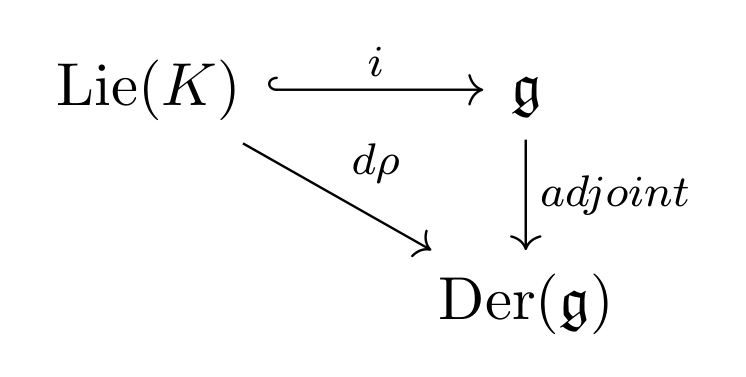
\includegraphics[width=0.30\linewidth]{fig_p087_1.png}
  \caption*{Harish--Chandra 对的相容性交换图（原文 PDF p.87 示意图，原文无编号）}
\end{figure}
\end{wdefn}

% [Tutor Note: 上述相容性的确切意思是 $d\rho=\operatorname{ad}\circ i$，其中
% $\operatorname{ad}:\mathfrak{g}\to\operatorname{Der}(\mathfrak{g})$ 是伴随作用；
% 它是“群作用与 Lie 代数作用相容”的无穷小形式。检验一个 $(\mathfrak{g},K)$ 对
% 是否合法，只需验证这一条交换性。]

\begin{wdefn}{9.15}
  一个 $(\mathfrak{g},K)$-模是一个向量空间 $V$，带有
  \begin{itemize}[leftmargin=1.6em,itemsep=0.2em]
    \item $K$ 在 $V$ 上的一个作用：$K\xrightarrow{\ \varphi\ }\mathrm{GL}(V)$；
    \item 一个 Lie 代数同态 $\mathfrak{g}\to\End(V)$，
  \end{itemize}
  使得二者相容：
  \begin{figure}[htbp]
  \centering
  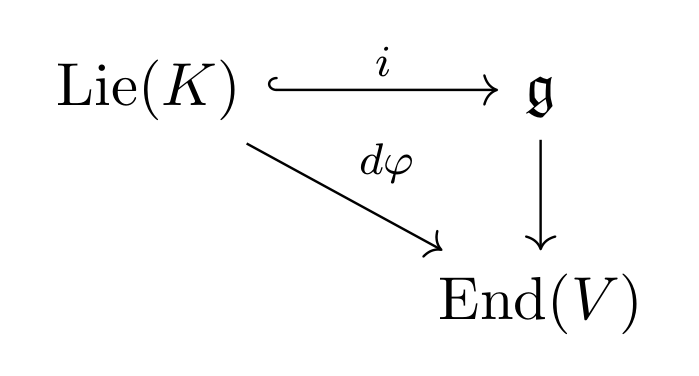
\includegraphics[width=0.28\linewidth]{fig_p087_2.png}
  \caption*{(g,K)-模的相容性交换图（原文 PDF p.87 示意图，原文无编号）}
\end{figure}
\end{wdefn}

\begin{wdefn}{9.16}
  $X$ 上的一个\textbf{平坦 $(\mathfrak{g},K)$-丛}是指
  \begin{itemize}[leftmargin=1.6em,itemsep=0.2em]
    \item 一个主 $K$-丛 $P\xrightarrow{\ \pi\ }X$；
    \item $P$ 上一个 $K$-等变的 $\mathfrak{g}$-值 1-形式
          $\gamma\in\Omega^1(P,\mathfrak{g})$，
  \end{itemize}
  且满足以下条件：
  \begin{enumerate}[label=(\arabic*),leftmargin=1.8em,itemsep=0.2em]
    \item 对任意 $a\in\operatorname{Lie}(K)$，设 $\xi_a\in\Vect(P)$ 是由 $a$ 生成的
          向量场。则缩并满足 $\gamma(\xi_a)=a$，且下图交换：
      \begin{figure}[htbp]
  \centering
  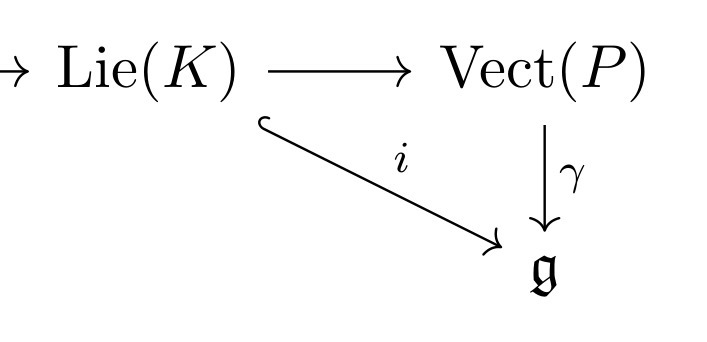
\includegraphics[width=0.28\linewidth]{fig_p087_3.png}
  \caption*{平坦 (g,K)-丛条件 (1) 的交换图（原文 PDF p.87 示意图，原文无编号）}
\end{figure}
% >>> p088
    \item $\gamma$ 满足 Maurer--Cartan 方程
      \[
        \dd\gamma+\frac{1}{2}[\gamma,\gamma]=0,
      \]
      其中 $\dd$ 是 $P$ 上的 de Rham 微分，$[-,-]$ 是 $\mathfrak{g}$ 中的 Lie 括号。
  \end{enumerate}
\end{wdefn}

% [Tutor Note: 条件 (1) 中 $\gamma(\xi_a)=a$ 表示 $\gamma$ 沿 $K$-轨道方向恰好等于
% 主丛联络的“垂直分量”；条件 (2) 的 Maurer--Cartan 方程是曲率为零的表述。注意
% $\frac12$ 因子与 $[\gamma,\gamma]$ 的约定必须一致：若把 $[\gamma,\gamma]$ 定义为
% $\gamma^a\wedge\gamma^b[T_a,T_b]$，则曲率为 $\dd\gamma+\frac12[\gamma,\gamma]$；
% 有些文献把 $\frac12$ 吸收进括号的定义，核对时务必确认，这是符号错误的高发点。]

给定平坦 $(\mathfrak{g},K)$-丛 $P\to X$ 与 $(\mathfrak{g},K)$-模 $V$，令
\[
  \Omega^\bullet(P,V):=\Omega^\bullet(P)\otimes V
\]
表示 $P$ 上取值于 $V$ 的微分形式。它带有一个联络
\[
  \nabla^\gamma=\dd+\gamma:\ \Omega^\bullet(P,V)\longrightarrow\Omega^{\bullet+1}(P,V),
\]
由 Maurer--Cartan 方程知该联络是平坦的。群 $K$ 作用在 $\Omega^\bullet(P)$ 与 $V$
上，从而在 $\Omega^\bullet(P,V)$ 上诱导一个自然作用。

令
\[
  V_P:=P\times_K V
\]
为 $X$ 上与 $K$-表示 $V$ 相伴的向量丛。设 $\Omega^\bullet(X;V_P)$ 表示 $X$ 上取值
于丛 $V_P\to X$ 的微分形式。与通常的主丛情形类似，$\nabla^\gamma$ 在 $V_P\to X$
上诱导一个平坦联络。这就定义了（de Rham）链复形
$(\Omega^\bullet(X;V_P),\nabla^\gamma)$，其相应的 de Rham 上同调记为
$H^\bullet(X;V_P)$。

下面我们讨论如何把 Lie 代数上同调下降为 $X$ 上的几何对象。

\begin{wdefn}{9.17}
  设 $V$ 是 $(\mathfrak{g},K)$-模。定义 $(\mathfrak{g},K)$ \textbf{相对 Lie 代数
  上链复形} $(C^\bullet_{\mathrm{Lie}}(\mathfrak{g},K;V),\partial_{\mathrm{Lie}})$ 为
  \[
    C^p_{\mathrm{Lie}}(\mathfrak{g},K;V)
    =\operatorname{Hom}_K\left(\wedge^p(\mathfrak{g}/\operatorname{Lie}(K)),V\right).
  \]
  这里 $\operatorname{Hom}_K$ 表示 $K$-等变线性映射。若把
  $C^p_{\mathrm{Lie}}(\mathfrak{g},K;V)$ 视为 Lie 代数上链
  $C^p_{\mathrm{Lie}}(\mathfrak{g};V)$ 的子空间，则 $\partial_{\mathrm{Lie}}$ 就是
  Chevalley--Eilenberg 微分。显式地，对
  $\alpha\in C^p_{\mathrm{Lie}}(\mathfrak{g},K;V)$，
  \[
    \begin{aligned}
      (\partial_{\mathrm{Lie}}\alpha)(a_1\wedge\cdots\wedge a_{p+1})
      ={}&\sum_{i=1}^{p+1}(-1)^{i-1}a_i\cdot
      \alpha\left(a_1\wedge\cdots\wedge\widehat{a_i}\wedge\cdots\wedge a_{p+1}\right)\\
      &+\sum_{i<j}(-1)^{i+j}\alpha\left([a_i,a_j]\wedge\cdots\wedge\widehat{a_i}
      \wedge\cdots\wedge\widehat{a_j}\wedge\cdots\wedge a_{p+1}\right).
    \end{aligned}
  \]
  相应的上同调记为 $H^\bullet_{\mathrm{Lie}}(\mathfrak{g},K;V)$。
\end{wdefn}

% [Tutor Note: Chevalley--Eilenberg 微分的符号约定：第一项 $(-1)^{i-1}$、第二项
% $(-1)^{i+j}$ 分别对应“把 $a_i$ 移到最前面”与“用 $[a_i,a_j]$ 替换两个变量”所需的
% Koszul 符号；不同教材可能相差一个整体符号，但上同调不受影响。另请注意相对复形中
% 除掉的是 $\operatorname{Lie}(K)$ 而非 $\mathfrak{h}$：二者只在
% $K=\mathrm{Sp}_{2n}$、$\operatorname{Lie}(K)=\mathfrak{sp}_{2n}$ 这类情形下才一致，
% 而定义 9.17 的记号 $(\mathfrak{g},K)$ 允许 $K$ 的 Lie 代数严格小于 $\mathfrak{g}$
% 中的另一个子代数 $\mathfrak{h}$。]

给定 $(\mathfrak{g},K)$-模 $V$ 与带有平坦联络 $\gamma\in\Omega^1(P,\mathfrak{g})$
的平坦 $(\mathfrak{g},K)$-丛 $P\to X$。我们可以定义从 $(\mathfrak{g},K)$ 相对 Lie
代数上链复形到 $P$ 上 $V$-值 de Rham 复形的\textbf{下降映射}（descent map）
\[
  \operatorname{desc}:\ \left(C^\bullet_{\mathrm{Lie}}(\mathfrak{g},K;V),
  \partial_{\mathrm{Lie}}\right)\longrightarrow\left(\Omega^\bullet(X;V_P),\nabla^\gamma\right),
  \qquad \alpha\mapsto\alpha(\gamma,\cdots,\gamma),
\]
并诱导上同调的下降映射
\[
  \operatorname{desc}:\ H^\bullet_{\mathrm{Lie}}(\mathfrak{g},K;V)
  \longrightarrow H^\bullet(X;V_P).
\]

% [Tutor Note: 原文此处说 “to $V$-valued de Rham complex on $P$”，但紧随的公式给出
% 的是 $X$ 上的复形 $(\Omega^\bullet(X;V_P),\nabla^\gamma)$；疑为笔误，应读作
% “on $X$”——$V_P$ 是 $X$ 上的丛，$\gamma$ 只用于把 $\alpha$ 沿 $\gamma$ 取值。
% 请核对原书 p.87（PDF p.88）。]

% >>> p089
\paragraph*{Fedosov 联络再探（Fedosov connection revisited）}

回忆（形式）Weyl 代数
\[
  \mathcal{W}_{2n}=\mathbb{R}[[p_i,q^i]]((\hbar)),\qquad
  \mathcal{W}^+_{2n}=\mathbb{R}[[p_i,q^i]][[\hbar]],
\]
带有诱导的 Lie 代数结构，其 Lie 括号定义为
\[
  [f,g]:=\frac{1}{\hbar}[f,g]_\star=\frac{1}{\hbar}(f\star g-g\star f).
\]

% [Tutor Note: 这里指标写作 $p_i$（下标）与 $q^i$（上标），是余切坐标的写法；
% 前文若出现 $q_i$ 只是指标升降的差别，核对公式时以原图为准。Lie 括号定义中的
% $\frac{1}{\hbar}$ 是为了让 $\star$ 的半经典极限恰好给出 Poisson 括号：
% 若采用 $f\star g=fg+\frac{\hbar}{2}\{f,g\}+\cdots$ 的 Moyal 约定，则
% $[f,g]=\{f,g\}+O(\hbar)$，符号取决于 $\star$ 的方向约定，此处极易差一个负号。]

设 $\mathrm{Sp}_{2n}$ 是保持 Poisson 双向量 $\Pi$ 的线性变换构成的辛群。它通过内
自同构作用在 Weyl 代数上。我们可以把 $\mathrm{Sp}_{2n}$ 的 Lie 代数
$\mathfrak{sp}_{2n}$ 与 $\mathbb{R}[p_i,q^i]$ 中的二次多项式等同起来，而
$\mathfrak{sp}_{2n}$ 是 $\mathcal{W}^+_{2n}$ 的 Lie 子代数。$\mathrm{Sp}_{2n}$ 在
$\mathbb{R}^{2n}$ 上的作用诱导出 $\mathrm{Sp}_{2n}$ 在 $\mathcal{W}^+_{2n}$ 上的
作用。因此，$(\mathcal{W}^+_{2n},\mathrm{Sp}_{2n})$ 与
$(\mathcal{W}_{2n},\mathrm{Sp}_{2n})$ 都是 Harish--Chandra 对。

设 $(X,\omega)$ 是辛流形，$F_{\mathrm{Sp}}(X)$ 是辛标架丛。我们有 Weyl 丛
\[
  \mathcal{W}^+_X=F_{\mathrm{Sp}}(X)\times_{\mathrm{Sp}_{2n}}\mathcal{W}^+_{2n},
  \qquad
  \mathcal{W}_X=F_{\mathrm{Sp}}(X)\times_{\mathrm{Sp}_{2n}}\mathcal{W}_{2n}.
\]
考虑 Harish--Chandra 对
\[
  (\bar{\mathfrak{g}},K)=(\mathfrak{g}/Z(\mathfrak{g}),\mathrm{Sp}_{2n}),
\]
其中 $\mathfrak{g}=\mathcal{W}^+_{2n}$，$Z(\mathfrak{g})=\mathbb{R}[[\hbar]]$ 是
$\mathfrak{g}$ 的中心，$Z(\mathfrak{g})\cap\mathfrak{sp}_{2n}=0$。Fedosov 构造了
平坦 $(\bar{\mathfrak{g}},K)$-丛 $F_{\mathrm{Sp}}(X)\to X$，而
$H^0(X;\mathcal{W}^+_X)$ 给出一个形变量子化。取平凡的
$(\bar{\mathfrak{g}},K)$-模 $\mathbb{R}((\hbar))$。则
\[
  \operatorname{desc}:\ C^\bullet_{\mathrm{Lie}}\left(\mathcal{W}^+_{2n},
  \mathfrak{sp}_{2n};\mathbb{R}((\hbar))\right)\longrightarrow\Omega^\bullet_X((\hbar)).
\]
这就是 Gelfand--Fuks 映射。这里
\[
  C^\bullet_{\mathrm{Lie}}\left(\mathcal{W}^+_{2n},\mathfrak{sp}_{2n};
  \mathbb{R}((\hbar))\right)
  \simeq C^\bullet_{\mathrm{Lie}}\left(\mathcal{W}^+_{2n},
  \mathfrak{sp}_{2n}\oplus Z(\mathcal{W}^+_{2n});\mathbb{R}((\hbar))\right).
\]

% [Tutor Note: Gelfand--Fuks（下降）映射的几何含义是：把相对 Lie 代数上链沿
% Fedosov 联络 $\gamma$ 取值，就得到 $X$ 上的微分形式，从而把纯代数的上同调类
% 送到几何对象上。最后一式的等号把 $\mathfrak{sp}_{2n}$ 换成
% $\mathfrak{sp}_{2n}\oplus Z(\mathcal{W}^+_{2n})$，可理解为把中心视为在复形上
% 作用平凡（作者在此采用简化记号）；若严格按
% $\operatorname{Hom}_{\mathfrak{h}}(\wedge^\bullet(\mathfrak{g}/\mathfrak{h}),-)$
% 的字面定义，商空间会变化，阅读时以作者原意为准。]

\paragraph*{示性类（Characteristic classes）}

我们来回顾 Lie 代数上同调中示性类的 Chern--Weil 构造。它们将经 Gelfand--Fuks
映射下降为通常的示性形式。

设 $\mathfrak{g}$ 是 Lie 代数，$\mathfrak{h}\subset\mathfrak{g}$ 是其 Lie 子代数。
设投影映射
\[
  \operatorname{pr}:\ \mathfrak{g}\longrightarrow\mathfrak{h}
\]
是嵌入 $\mathfrak{h}\subset\mathfrak{g}$ 的 $\mathfrak{h}$-等变分裂。一般来说，
$\operatorname{pr}$ 不是从 $\mathfrak{g}$ 到 $\mathfrak{h}$ 的 Lie 代数同态。
$\operatorname{pr}$ 不是 Lie 代数同态这一事实给出
$R\in\operatorname{Hom}(\wedge^2\mathfrak{g},\mathfrak{h})$：
\[
  R(\alpha,\beta)=[\operatorname{pr}(\alpha),\operatorname{pr}(\beta)]_{\mathfrak{h}}
  -\operatorname{pr}[\alpha,\beta]_{\mathfrak{g}},\qquad \alpha,\beta\in\mathfrak{g}.
\]
$\operatorname{pr}$ 的 $\mathfrak{h}$-等变性蕴含
$R\in\operatorname{Hom}_{\mathfrak{h}}(\wedge^2(\mathfrak{g}/\mathfrak{h}),\mathfrak{h})$。
$R$ 称为\textbf{曲率形式}。设 $\operatorname{Sym}^m(\mathfrak{h}^\vee)^{\mathfrak{h}}$
是 $\mathfrak{h}$ 上齐次次数为 $\deg=m$ 的 $\mathfrak{h}$-不变多项式。给定
$P\in\operatorname{Sym}^m(\mathfrak{h}^\vee)^{\mathfrak{h}}$，我们可以通过复合
\[
  P(R):\ \wedge^{2m}\mathfrak{g}\xrightarrow{\ \wedge^m R\ }
  \operatorname{Sym}^m(\mathfrak{h})\xrightarrow{\ P\ }\mathbb{R}
\]
联系一个上链 $P(R)\in C^{2m}_{\mathrm{Lie}}(\mathfrak{g},\mathfrak{h};\mathbb{R})$。

% [Tutor Note: 这里 $R$ 取值于 $\mathfrak{h}$ 而非 $\mathfrak{g}$，且只在
% $\wedge^2(\mathfrak{g}/\mathfrak{h})$ 上有定义；改变分裂 $\operatorname{pr}$
% 会使 $R$ 改变一个 $\mathfrak{h}$-等变的上链，故下文的上同调类与 $\operatorname{pr}$
% 的选取无关——这正是 Chern--Weil 理论中“曲率形式依赖联络、示性类不依赖联络”
% 的 Lie 代数类比。]

% >>> p090
可以验证 $\partial_{\mathrm{Lie}}P(R)=0$，这在上同调
$H^{2m}(\mathfrak{g},\mathfrak{h};\mathbb{R})$ 中定义一个不依赖于
$\operatorname{pr}$ 选取的上同调类 $[P(R)]$。因此我们得到 Chern--Weil 示性映射的
类比
\[
  \chi:\ \operatorname{Sym}^\bullet(\mathfrak{h}^\vee)^{\mathfrak{h}}
  \longrightarrow H^\bullet(\mathfrak{g},\mathfrak{h};\mathbb{R}),
  \qquad P\mapsto\chi(P):=[P(R)].
\]
现在把上述构造应用于
\[
  \mathfrak{g}=\mathcal{W}^+_{2n},\qquad
  \mathfrak{h}=\mathfrak{sp}_{2n}\oplus Z(\mathfrak{g})
\]
的情形。$\mathfrak{g}=\mathcal{W}^+_{2n}$ 中任意元素 $f$ 都可唯一地写成多项式
$f=f(y^i,\hbar)$，其中坐标取为
\[
  (y^1,\cdots,y^n,y^{n+1},\cdots,y^{2n})=(p_1,\cdots,p_n,q^1,\cdots,q^n).
\]
定义 $\mathfrak{h}$-等变投影
\[
  \operatorname{pr}_1(f)=\frac{1}{2}\sum_{i,j}
  \partial_i\partial_j f\Big|_{y=\hbar=0}\,y^iy^j\in\mathfrak{sp}_{2n},
  \qquad
  \operatorname{pr}_3(f)=f|_{y=0}\in Z(\mathfrak{g}).
\]
我们得到相应的曲率
\[
  \begin{aligned}
    R_1&:=[\operatorname{pr}_1(-),\operatorname{pr}_1(-)]
    -\operatorname{pr}_1[-,-]\in\operatorname{Hom}(\wedge^2\mathfrak{g},\mathfrak{sp}_{2n}),\\
    R_3&:=-\operatorname{pr}_3[-,-]\in\operatorname{Hom}(\wedge^2\mathfrak{g},\mathbb{R}[[\hbar]]).
  \end{aligned}
\]

\begin{wrem}{9.18}
  当我们并入向量丛时，可以考虑更一般的情形：此时
  \[
    \mathfrak{g}=\mathcal{W}^+_{2n}+\hbar\left(\mathfrak{gl}(\mathcal{W}^+_{2n})\right),
    \qquad
    \mathfrak{h}=\mathfrak{sp}_{2n}\oplus\hbar\mathfrak{gl}\oplus Z(\mathfrak{g}).
  \]
  其中多出的投影 $\operatorname{pr}_2$ 及其相应的曲率 $R_2$ 分别定义为
  $\hbar\mathfrak{gl}$ 与 $\operatorname{Hom}(\wedge^2,\mathfrak{gl})$ 中的元素。
  值得指出的是，这里所有的 $\operatorname{Hom}$ 都只是 $\mathbb{R}$-线性的映射，
  而不是 $\mathbb{R}[[\hbar]]$-线性的，尽管 $\mathfrak{g}$ 是一个
  $\mathbb{R}[[\hbar]]$-模。
\end{wrem}

% [Tutor Note: 注 9.18 中 “$\operatorname{Hom}(\wedge^2,\mathfrak{gl})$” 省略了
% 第一个变量 $\mathfrak{g}$，应读作 $\operatorname{Hom}(\wedge^2\mathfrak{g},
% \mathfrak{gl})$；$\mathfrak{g}=\mathcal{W}^+_{2n}+\hbar\,\mathfrak{gl}
% (\mathcal{W}^+_{2n})$ 中的加号表示把矩阵值系数并入 Weyl 代数（半直和），并非
% 通常的直和记号的用法。原文照录，特此说明。]

我们现定义 $\widehat{A}$-亏格
\[
  \widehat{A}(\mathfrak{sp}_{2n}):=\left[\det\left(\frac{R_1/2}
  {\sinh(R_1/2)}\right)^{\frac{1}{2}}\right]\in H^\bullet(\mathfrak{g},\mathfrak{h};\mathbb{R}).
\]

\begin{wprop}{9.19}
  在经 Fedosov 联络的下降映射
  $\operatorname{desc}:H^\bullet(\mathfrak{g},\mathfrak{h};\mathbb{R}((\hbar)))
  \to H^\bullet(X)((\hbar))$ 之下，有
  \[
    \operatorname{desc}\left(\widehat{A}(\mathfrak{sp}_{2n})\right)=\widehat{A}(X),
    \qquad
    \operatorname{desc}(R_3)=\omega_\hbar-\hbar\omega.
  \]
\end{wprop}

% [Tutor Note: $\widehat{A}$-亏格中的 $R_1$ 是 $\mathfrak{sp}_{2n}$-值 2-形式，
% $\det$ 与 $\sinh$ 都在矩阵意义下取，外层的 $\frac12$ 次幂与外层方括号（表示
% 上同调类）都是定义的一部分，不可漏写。$\operatorname{desc}(R_3)=\omega_\hbar
% -\hbar\omega$ 中 $\omega_\hbar$ 是 $\hbar$-修正后的辛形式（Fedosov 构造的
% 标准输出，见 [24]），代入指标公式时它决定 $\ee^{-\omega_\hbar/\hbar}$ 的系数。]

\paragraph*{万有迹映射（Universal trace map）}

回忆利用 $\Omega^\bullet_{S^1}\to\mathbb{R}^{2n}$，我们已得到
\[
  \operatorname{Tr}=\int_{BV}\circ\langle-\rangle_{\mathrm{free}}:\
  CC^{\mathrm{per}}_{-\bullet}(\mathcal{W}_{2n})\longrightarrow
  K:=\mathbb{R}((\hbar))[u,u^{-1}].
\]
我们把它写成
\[
  \operatorname{Tr}\in\operatorname{Hom}_K\left(CC^{\mathrm{per}}_{-\bullet}
  (\mathcal{W}_{2n}),K\right).
\]
这是一个 $(\mathcal{W}^+_{2n},\mathrm{Sp}_{2n})$-模。经平坦
$(\mathcal{W}^+_{2n},\mathrm{Sp}_{2n})$-丛 $F_{\mathrm{Sp}}(X)\to X$，我们得到
相伴丛
\[
  E^{\mathrm{per}}:=F_{\mathrm{Sp}}(X)\times_{\mathrm{Sp}_{2n}}
  \operatorname{Hom}_K\left(CC^{\mathrm{per}}_{-\bullet}(\mathcal{W}_{2n}),K\right)
\]
% >>> p091
带有诱导的平坦联络 $\nabla^\gamma$。

回忆 Weyl 丛 $\mathcal{W}(X)=F_{\mathrm{Sp}}(X)\times_{\mathrm{Sp}_{2n}}
\mathcal{W}_{2n}$ 带有平坦联络 $\nabla^\gamma$。我们想把 $\operatorname{Tr}$
粘合到 $X$ 上。记 $\delta$ 为 $\operatorname{Hom}_K\left(CC^{\mathrm{per}}_{-\bullet}
(\mathcal{W}_{2n}),K\right)$ 上由 $b+uB$ 诱导的微分。于是
\[
  \delta\operatorname{Tr}=\operatorname{Tr}\left((b+uB)(-)\right)=0.
\]
我们可以把 $\operatorname{Tr}$ 看作定义了
\[
  C^0_{\mathrm{Lie}}\left(\mathfrak{g},\mathfrak{h};\operatorname{Hom}_K
  \left(CC^{\mathrm{per}}_{-\bullet}(\mathcal{W}_{2n}),K\right)\right)
\]
中的一个元素，其中取
\[
  \mathfrak{g}=\mathcal{W}^+_{2n}/Z(\mathcal{W}^+_{2n}),\qquad
  \mathfrak{h}=\mathfrak{sp}_{2n}.
\]
然而 $\operatorname{Tr}$ 不是 $\mathfrak{g}$-不变的，即
$\partial_{\mathrm{Lie}}\operatorname{Tr}\neq0$。换言之，$\operatorname{Tr}$ 不是
$(\mathfrak{g},\mathrm{Sp}_{2n})$-模之间的映射。因此 $\operatorname{Tr}$ 不能
直接粘合。

% [Tutor Note: $\delta$ 是由 $b+uB$ 在 $\operatorname{Hom}_K(CC^{\mathrm{per}}_{-\bullet}
% (\mathcal{W}_{2n}),K)$ 上诱导的微分；$b+uB$ 正是周期循环链复形的微分，故
% $\delta\operatorname{Tr}=0$ 表示 $\operatorname{Tr}$ 是（取值于 $K$ 的）循环链的
% 迹。原文 “$\partial_{\mathrm{Lie}}\operatorname{Tr}=\delta(-)$” 是简写，意为
% $\partial_{\mathrm{Lie}}\operatorname{Tr}$ 是某个元素的 $\delta$-像，而不是等于
% $\delta$ 算子本身；照录原文，阅读时注意。]

我们注意到 $\partial_{\mathrm{Lie}}\operatorname{Tr}=\delta(-)$。事实表明，存在
一种典范的方式把 $\operatorname{Tr}$ 提升为
\[
  \widehat{\operatorname{Tr}}\in C^\bullet_{\mathrm{Lie}}\left(\mathfrak{g},\mathfrak{h};
  \operatorname{Hom}_K\left(CC^{\mathrm{per}}_{-\bullet}(\mathcal{W}_{2n}),K\right)\right),
\]
使得
\[
  \widehat{\operatorname{Tr}}=\operatorname{Tr}
  +\ C^{>0}_{\mathrm{Lie}}\left(\mathfrak{g},\mathfrak{h};\operatorname{Hom}_K
  \left(CC^{\mathrm{per}}_{-\bullet}(\mathcal{W}_{2n}),K\right)\right)\ \text{中的项},
\]
并满足耦合上闭链条件
\[
  (\partial_{\mathrm{Lie}}+\delta)\widehat{\operatorname{Tr}}=0.
\]
$\widehat{\operatorname{Tr}}$ 称为\textbf{万有迹映射}。让我们代入
$1\in\mathcal{W}_{2n}$，则 $\widehat{\operatorname{Tr}}(1)$ 是
$\partial_{\mathrm{Lie}}$-闭的，从而定义\textbf{万有指标}
\[
  \left[\widehat{\operatorname{Tr}}(1)\right]
  \in H^\bullet_{\mathrm{Lie}}(\mathfrak{g},\mathfrak{h};K).
\]

\begin{wthm}{9.20}（万有代数指标定理（Universal algebraic index theorem））
  \[
    \left[\widehat{\operatorname{Tr}}(1)\right]
    =u^ne^{-R_3/(u\hbar)}\widehat{A}(\mathfrak{sp}_{2n})_u,
  \]
  其中对 $A=\sum_{p\ \text{even}}A_p$，$A_p\in H^p(\mathfrak{g},\mathfrak{h};K)$，
  定义
  \[
    A_u=\sum_p u^{-p/2}A_p.
  \]
\end{wthm}

% [Tutor Note: 定理中的 $u^n$ 与 $A_u=\sum_p u^{-p/2}A_p$ 表明该指标是 $u$ 的半整数
% 次幂的 Laurent 级数；$e^{-R_3/(u\hbar)}$ 的分母 $u\hbar$ 不可与下文
% $e^{-\omega_\hbar/\hbar}$ 的分母混淆。此处 $[\cdot]$ 表示相对 Lie 代数上同调类；
% 整体化（PDF p.92）后即得 $\int_X\ee^{-\omega_\hbar/\hbar}\widehat{A}(X)$，这正是
% Atiyah--Singer 指标定理的 $\widehat{A}$-形式在形变量子化中的类比。]

该定理由 Feigin--Tsygan [20]、Feigin--Felder--Shoikhet [19]、
Bressler--Nest--Tsygan [8] 等人的工作发展而来，并可自然地推广到向量丛的情形 [24]。

现在对 $\widehat{\operatorname{Tr}}$ 应用 Gelfand--Fuks（下降）映射，使得
\begin{figure}[htbp]
  \centering
  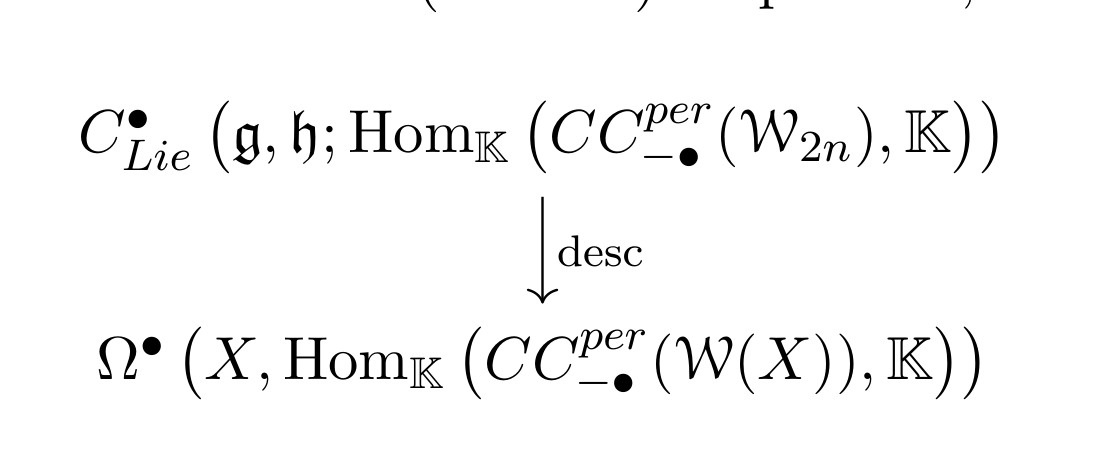
\includegraphics[width=0.45\linewidth]{fig_p091_1.png}
  \caption*{Gelfand--Fuks 下降映射的纵向箭头（原文 PDF p.91 示意图，原文无编号）}
\end{figure}
设 $\mathcal{W}_D(X)$ 是 $\mathcal{W}(X)$ 的平坦截面空间，它给出一个形变量子化。
则
\[
  \operatorname{desc}(\widehat{\operatorname{Tr}}):\
  CC^{\mathrm{per}}_{-\bullet}(\mathcal{W}_D(X))\longrightarrow
  \Omega^\bullet(X)((\hbar))[u,u^{-1}],\qquad b+uB\mapsto \dd_X.
\]

% >>> p092
特别地，它通过
\[
  f\in\mathcal{W}_D(X)\longmapsto\int_X\operatorname{desc}
  (\widehat{\operatorname{Tr}})(f)\in\mathbb{R}((\hbar))
\]
在形变量子化中定义一个迹映射。可以证明
$\int_X\operatorname{desc}(\widehat{\operatorname{Tr}})(f)$ 不涉及 $u$。由万有
代数指标定理，我们有
\[
  \int_X\operatorname{desc}(\widehat{\operatorname{Tr}})(1)
  =\int_X\ee^{-\omega_\hbar/\hbar}\widehat{A}(X).
\]
这就给出\textbf{代数指标定理}。

% [Tutor Note: “$\int_X\operatorname{desc}(\widehat{\operatorname{Tr}})(f)$ 不涉及
% $u$” 是说积分后 $u$ 的依赖消失（相应的项为恰当形式/整体上消失），故得到与 $u$
% 无关的数值不变量；这是把循环同调的迹下降为普通数值迹的关键一步。整体公式
% $\int_X\ee^{-\omega_\hbar/\hbar}\widehat{A}(X)$ 与代数指标定理的标准形式一致，
% $\hbar\to0$ 时给出 $\int_X\widehat{A}(X)$ 这一拓扑指标。]

\paragraph*{万有迹映射 $\widehat{\operatorname{Tr}}$ 的构造（Construction of universal trace map $\widehat{\operatorname{Tr}}$）}

我们有如下关系。
\begin{figure}[htbp]
  \centering
  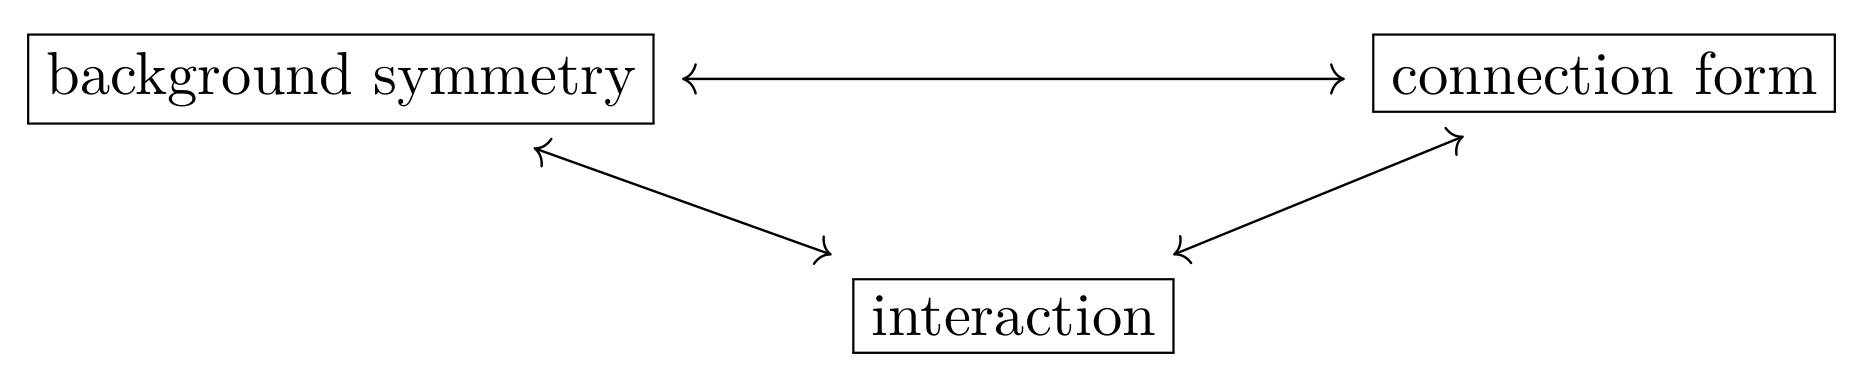
\includegraphics[width=0.75\linewidth]{fig_p092_1.png}
  \caption*{背景对称性、联络形式与相互作用之间的关系（原文 PDF p.92 示意图，原文无编号）}
\end{figure}
设 $\Theta:\mathfrak{g}\to\mathcal{W}^+_{2n}/Z(\mathcal{W}^+_{2n})
=\bar{\mathfrak{g}}$ 是典范恒等映射。对每个
$f\in\mathcal{W}^+_{2n}/Z(\mathcal{W}^+_{2n})$，我们已在
$\mathcal{E}=\Omega^\bullet(S^1)\otimes\mathbb{R}^{2n}$ 上定义局部泛函
\[
  I_f(\varphi)=\int_{S^1}f(\varphi),\qquad \varphi\in\mathcal{E}.
\]
于是 $\Theta$ 给出映射
\[
  I_\Theta:\ \mathfrak{g}\longrightarrow\mathcal{O}_{\mathrm{loc}}(\mathcal{E}),
  \qquad f\mapsto I_{\Theta(f)}.
\]
我们可以把这个映射看作
\[
  I_\Theta\in C^1(\mathfrak{g},\mathcal{O}_{\mathrm{loc}}(\mathcal{E}))
  =\mathfrak{g}^\vee\otimes\mathcal{O}_{\mathrm{loc}}(\mathcal{E}).
\]
现在可以构造
$\widehat{\operatorname{Tr}}\in C^\bullet_{\mathrm{Lie}}\left(\mathfrak{g},
\mathfrak{h};\operatorname{Hom}_K\left(CC^{\mathrm{per}}_{-\bullet}
(\mathcal{W}_{2n}),K\right)\right)$ 如下：
\[
  \begin{aligned}
    \widehat{\operatorname{Tr}}(f_0\otimes f_1\otimes\cdots\otimes f_m)
    &:=\int_{BV}\exp\left(\hbar P_0^\infty\right)\left(\mathcal{O}_{f_0,f_1,\cdots,f_m}
    \ee^{\frac{1}{\hbar}I_\Theta}\right)
    \in C^\bullet(\mathfrak{g},\mathfrak{h};K),\qquad f_i\in\mathcal{W}_{2n}\\
    &\text{``}=\int_{BV}\int_{\operatorname{Im}\dd^*\subset\mathcal{E}}
    \ee^{-\frac{1}{2\hbar}\int_{S^1}\langle\varphi,\dd\varphi\rangle
    +\frac{1}{\hbar}I_\Theta}\mathcal{O}_{f_0,f_1,\cdots,f_m}\text{''}.
  \end{aligned}
\]

% [Tutor Note: 原文 “Let $\Theta:\mathfrak{g}\to\mathcal{W}^+_{2n}/Z(\mathcal{W}^+_{2n})
% =\bar{\mathfrak{g}}$ be the canonical identity map” 中，$\Theta$ 严格说不是恒等映射
% （定义域与值域不同），而是把 $\mathfrak{g}=\mathcal{W}^+_{2n}$ 等同于商
% $\bar{\mathfrak{g}}$ 的典范等同/商映射；照录原文记号，阅读时按“商映射”理解。
% 第二行首尾的引号表示这是经过 Gauss 积分（对 $\operatorname{Im}d^*\subset
% \mathcal{E}$ 上的场）之后的形式表达式，并非逐字恒等；$P_0^\infty$ 是前文
% （9.1–9.4 节）同伦 RG 流中的传播子。]

\paragraph*{指标的计算（Computation of index）}

Weyl 代数 $\mathcal{W}_{2n}$ 可以看作以 $\hbar$ 为参数的一族结合代数。这导致
\textbf{Gauss--Manin--Getzler 联络} $\nabla_{\hbar\partial_\hbar}$ 作用在
$CC^{\mathrm{per}}_{-\bullet}(\mathcal{W}_{2n})$ 上。指标的计算由以下步骤组成：
\begin{enumerate}[label=(\arabic*),leftmargin=1.8em,itemsep=0.3em]
  \item \emph{Feynman 图计算}给出
    \[
      \widehat{\operatorname{Tr}}(1)=u^ne^{-R_3/(u\hbar)}
      \left(\underbrace{\widehat{A}(\mathfrak{sp}_{2n})_u}_{\text{单圈计算}}
      +O(\hbar)\right).
    \]
  \item \emph{Gauss--Manin--Getzler 联络}的计算表明
    $\nabla_{\hbar\partial_\hbar}\left(\ee^{R_3/(u\hbar)}
    \widehat{\operatorname{Tr}}(1)\right)$ 是 $\partial_{\mathrm{Lie}}$-恰当的。
  \item 结合 (1) 与 (2)，我们得到
    \[
      \left[\widehat{\operatorname{Tr}}(1)\right]
      =\left[u^ne^{-R_3/(u\hbar)}\widehat{A}(\mathfrak{sp}_{2n})_u\right]
      \in H^\bullet(\mathfrak{g},\mathfrak{h};K).
    \]
\end{enumerate}

% [Tutor Note: 第 (1) 步下括号“单圈计算”指出：$\widehat{A}$-亏格来自单圈 Feynman
% 图的和，而高圈项 $O(\hbar)$ 不改变上同调类；第 (2) 步用 Gauss--Manin--Getzler
% 联络（Getzler 在热核证明中引入的联络在循环同调上的版本）说明
% $\ee^{R_3/(u\hbar)}\widehat{\operatorname{Tr}}(1)$ 的协变导数恰当，从而第 (1) 步
% 的结果可以代表整个上同调类。三步合起来正是“局部单圈计算 + 整体下降 = 指标定理”
% 的标准论证结构。]


% ---------- part13.tex ----------
% ============================================================
%  part13.tex  |  原文 PDF p.93–101（页脚 p.92–100）
%  内容：第 10 章 二维手征量子场论（10.1–10.6，含定理 10.12）
%  说明：p.101 的 Theorem 10.12 属正文；其后的 References 由 Lead 处理，本片段不重复。
% ============================================================

% 正则化积分记号 \fint 已在 preamble.tex 中统一定义（不再在片段内兜底）。

% >>> p093
\section{二维手征量子场论（Two-dim Chiral QFT）}

\begin{keypoints}
  \item \textbf{核心物理图像}：二维手征模型的场是复微分形式
        $\Omega^{0,\bullet}(\Sigma,h)$，Dolbeault 微分 $\bar\partial$ 成为 BRST
        算子的一部分，使“反全纯平移在同调意义下平凡”，由此得到手征（全纯）理论；
        一维的“融合”升级为顶点代数的无穷族乘积 $A_{(n)}B$。
  \item \textbf{数学工具}：顶点代数与算子乘积展开（OPE）、模式 Lie 代数、
        Szegő 核、正则化积分 $\fint_\Sigma$、Beilinson--Drinfeld 手征代数与
        手征同调、BV 量子化。
  \item \textbf{主要结论}：$\beta\gamma$-$bc$ 系统的手征形变是紫外（UV）有限的
        （定理 10.4）；有效 QME 的解等价于 $[\oint\gamma,\oint\gamma]=0$
        （定理 10.6）；手征关联函数是几乎全纯模的，其反全纯依赖由全纯反常方程
        控制（定理 10.12）。
  \item \textbf{译者评注}：本章把第 8--9 章的一维 TQM 框架整体提升到二维：
        Hochschild 同调 $\to$ 手征同调，Fedosov 联络 $\to$ 手征 Fedosov 联络。
        技术核心是“看似发散的图积分可用共形结构内蕴正则化”，其中正则化积分的
        分解 $\omega=\alpha+\partial\beta$ 与留数性质是理解 UV 有限性的钥匙。
\end{keypoints}

我们已经讨论过拓扑量子力学的一阶形式，其中场是 $S^1$ 上取值于向量丛 $V$ 的
微分形式 $\Omega^\bullet(S^1,V)$，并配备 de Rham 微分 $d$。这里 $d$ 成为 BRST
算子的一部分，意味着“平移在同调意义下是平凡的”。这定义了一个拓扑理论。

% [Tutor Note: 一句话点明两种理论的“BRST 算子”差异：TQM 中进入 BRST 的是 de Rham
% 微分 $d$，它把平移方向（沿 $S^1$）变成同调平凡的；二维手征理论中进入 BRST 的是
% Dolbeault 微分 $\bar\partial$，它只消灭反全纯平移方向，因此理论只保留全纯（手征）
% 的依赖。读后文时务必区分 $\partial$（全纯 de Rham 微分）与 $\bar\partial$
% （Dolbeault 微分）——原书有时把两者都简单写作 $d$，是常见的记号陷阱。]

现在考虑二维手征模型，其中场是复微分形式 $\Omega^{0,\bullet}(\Sigma,h)$，配备
Dolbeault 微分 $\bar\partial$。$\bar\partial$ 成为 BRST 算子的一部分，意味着
“反全纯平移在同调意义下是平凡的”，这反过来定义了一个手征（或全纯）理论。

在拓扑量子力学中，理论是紫外（UV）有限的。第 7.4 节的一般讨论适用，我们发现
重整化后的 QME 转化为 Moyal 交换子与 Fedosov 方程。我们将会看到二维手征理论
同样是 UV 有限的，并且对 QME 有类似的几何结论 [29]。

\subsection{顶点代数（Vertex algebra）}

正如 1.2 节所讨论的，在一维拓扑理论中我们有由融合 $a\cdot b$ 定义的结合代数；
在二维手征理论中我们有由 $A_{(n)}B$ 定义的（手征）顶点代数。这些代数出现在
一个算子逼近另一个算子的情形——一维时在直线上，二维时在平面上。

\begin{figure}[htbp]
  \centering
  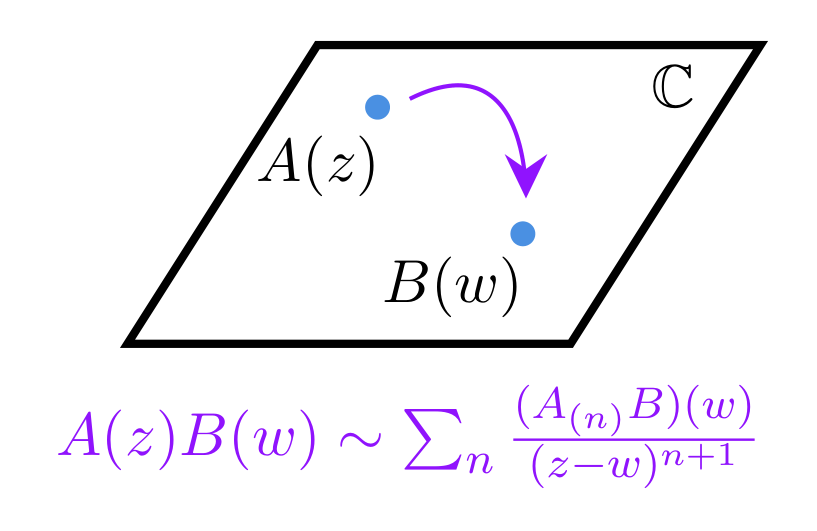
\includegraphics[width=0.33\linewidth]{fig_p093_1.png}
  \caption*{一维结合代数与二维顶点代数的乘积示意（原文 PDF p.93 示意图，原文无编号）}
\end{figure}

在平面上，“乘积”（二元运算）全纯地依赖于位置，从而导致无穷多个二元运算。

\begin{wdefn}{10.1}
  \textbf{顶点代数}是如下一组数据：
  \begin{itemize}[leftmargin=1.6em,itemsep=0.15em]
    \item （态空间）一个 $\mathbb{Z}$-分次超空间
          $\mathcal{V}=\mathcal{V}_0\oplus\mathcal{V}_1$，
    \item （真空）一个向量 $|0\rangle\in\mathcal{V}_0$，
    \item （平移算子）一个偶线性映射 $T:\mathcal{V}\to\mathcal{V}$，
    \item （态–场对应）一个偶线性运算（顶点运算）
          \[
            Y(-,z):\ \mathcal{V}\longrightarrow\End\mathcal{V}[[z,z^{-1}]],
            \qquad
            A\mapsto Y(A,z)=\sum_{n\in\mathbb{Z}}A_{(n)}z^{-n-1},
          \]
          使得对任意 $A,B\in\mathcal{V}$ 有 $Y(A,z)B\in\mathcal{V}((z))$。
  \end{itemize}
  这些数据要求满足以下公理：
  \begin{itemize}[leftmargin=1.6em,itemsep=0.15em]
    \item （真空公理）$Y(|0\rangle,z)=1_{d\mathcal{V}}$，即对任意
          $A\in\mathcal{V}$，
          \[
            Y(A,z)|0\rangle\in\mathcal{V}[[z]]
            \qquad\text{且}\qquad
            \lim_{z\to0}Y(A,z)|0\rangle=A,
          \]
    \item （平移公理）$T|0\rangle=0$，即对任意 $A\in\mathcal{V}$，
          \[
            [T,Y(A,z)]=\partial_zY(A,z),
          \]
% >>> p094
    \item （局域性公理）所有 $\{Y(A,z)\}_{a\in\mathcal{V}}$ 相互局域。
  \end{itemize}
\end{wdefn}

% [Tutor Note: 定义 10.1 中有两处原文笔误，均照录：其一，真空公理写作
% $Y(|0\rangle,z)=1_{d\mathcal{V}}$，其中 $1_{d\mathcal{V}}$ 记号可疑（疑为恒等
% 算子 $1_{\mathcal{V}}$ 或 $\mathrm{id}_{\mathcal{V}}$ 之误），按标准公理应理解为
% $\mathcal{V}$ 上的恒等算子；其二，局域性公理的下标是 $\{Y(A,z)\}_{a\in\mathcal{V}}$，
% 元素写作 $A$ 而下标却用 $a$（应为 $A\in\mathcal{V}$）。局域性是指任取 $A,B$，
% 存在 $N\ge0$ 使 $(z-w)^NY(A,z)Y(B,w)$ 无极点；它与真空公理、平移公理合起来
% 等价于 Borcherds（Jacobi）恒等式，原书未展开证明，可参阅 [5]。
% 请核对原书 p.92（PDF p.93）。]

粗略地说，相互局域性蕴含着：对任意 $A,B\in\mathcal{V}$，可以展开为
\[
  Y(A,z)Y(B,w)=\sum_{n\in\mathbb{Z}}\frac{Y(A_{(n)}\cdot B,w)}{(z-w)^{n+1}}.
\]
这称为\textbf{算子乘积展开}（operator product expansion, OPE）。展开系数
$\{A_{(n)}\cdot B\}$ 可视为定义了一族无穷多个乘积。为简便起见，对
$A\in\mathcal{V}$ 我们将记
\[
  A(z)\equiv Y(A,z).
\]
于是 OPE 可以写成
\[
  A(z)B(w)=\sum_{n\in\mathbb{Z}}\frac{A_{(n)}\cdot B(w)}{(z-w)^{n+1}}.
\]
当只关心奇异部分时，我们也写作
\[
  A(z)B(w)\sim\sum_{n\ge0}\frac{A_{(n)}\cdot B(w)}{(z-w)^{n+1}}.
\]

% [Tutor Note: OPE 的分母幂次 $(z-w)^{n+1}$ 与模式展开 $A(z)=\sum A_{(n)}z^{-n-1}$
% 是同一约定下的配套写法：围道积分 $\oint\dd z\,z^mA(z)$ 正好挑出模式 $A_{(m)}$。
% 不同文献常把分母写成 $(z-w)^{-n-1}$ 并对 $n$ 作相反编号，或把模式记作
% $A_n$（对应 $z^{-n-h}$，$h$ 为共形权重），二者只差重编号/平移；核对公式时先看
% 分母幂次是 $n+1$ 还是 $-n-1$，这是本章最容易出错的地方。]

给定顶点代数，我们可以定义其\textbf{模式 Lie 代数}
\[
  \oint\mathcal{V}:=\operatorname{Span}_{\mathbb{C}}
  \left\{\oint\dd z\,z^kA(z)=A_{(k)}\right\}_{A\in\mathcal{V},\,k\in\mathbb{Z}}.
\]
围道积分的 Lie 括号由 OPE 决定：
\[
  \left[\oint\dd z\,z^mA(z),\oint\dd w\,w^nB(w)\right]
  =\oint\dd w\,w^n\oint_w\dd z\,z^m
  \sum_{j\in\mathbb{Z}}\frac{A_{(j)}\cdot B(w)}{(z-w)^{j+1}},
\]
其中积分中只有奇异部分起作用。该 Lie 括号可用图形表示如下。

% [Tutor Note: $\oint_w$ 表示以 $w$ 为圆心的小围道，且外层积分先做；右端的括号
% 是“先算内部 OPE 再取围道积分”的结果。注意围道的嵌套次序不能随意交换——交换
% 次序会产生额外的收缩项，这正是 OPE 中奇异部分的来源；图形表示（下图）正是把
% 交换子画成两种嵌套方式之差。]

\begin{figure}[htbp]
  \centering
  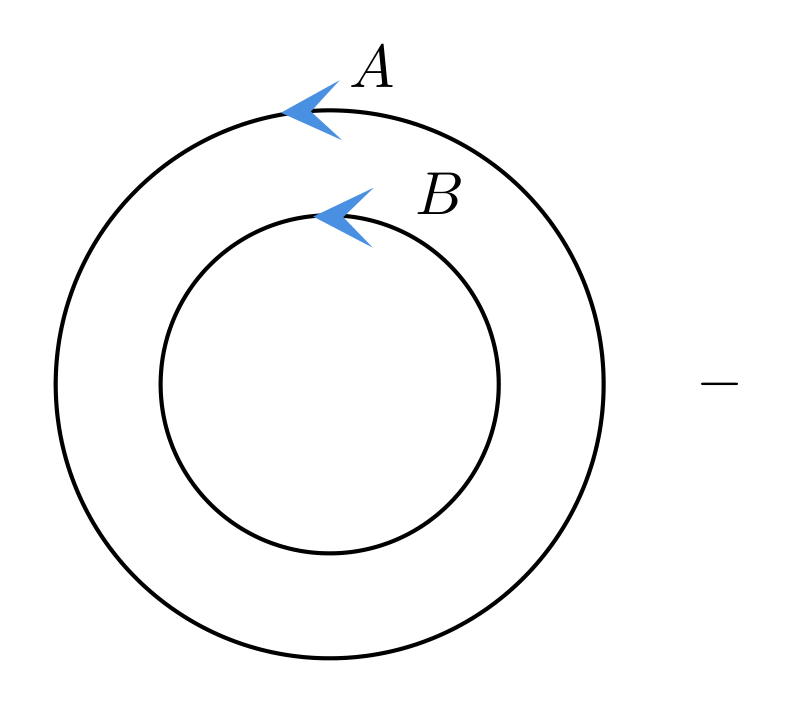
\includegraphics[width=0.32\linewidth]{fig_p094_1.png}
  \caption*{围道积分的 Lie 括号的图形表示（原文 PDF p.94 示意图，原文无编号）}
\end{figure}

\begin{wexam}{10.2}（$\beta\gamma$ 系统）
  $\beta\gamma$ 系统由两个玻色场 $\beta(z),\gamma(z)$ 生成，其缩并（contractions）为
  \[
    \beta(z)\gamma(w)\sim\frac{\hbar}{z-w}\sim-\gamma(z)\beta(w).
  \]
  顶点代数 $\mathcal{V}$ 等同于微分环
  \[
    \mathcal{V}=:\mathbb{C}[[\partial^i\beta,\partial^i\gamma]]:[[\hbar]],
  \]
% >>> p095
  其中 $::$ 是正规序算子。一般的 OPE 由 \textbf{Wick 缩并}得到。例如，
  \[
    \begin{aligned}
      :\beta(z)\gamma(z)::\beta(w)\gamma(w):
      ={}&\underbrace{\frac{\hbar}{z-w}:\gamma(z)\beta(w):
      -\frac{\hbar}{z-w}:\beta(z)\gamma(w):}_{\text{1 次缩并}}\\
      &-\underbrace{\left(\frac{\hbar}{z-w}\right)^{2}}_{\text{2 次缩并}}\\
      ={}&\sum_{k\ge0}\frac{\hbar}{z-w}\frac{(z-w)^k}{k!}
      :\partial^k\gamma(w)\beta(w)-\partial^k\beta(w)\gamma(w):
      -\frac{\hbar^2}{(z-w)^2}.
    \end{aligned}
  \]
\end{wexam}

% [Tutor Note: 两个缩并公式的符号差异来自统计性质：$\beta,\gamma$ 是玻色场，交换
% 不产生符号，故 $\beta(z)\gamma(w)\sim\frac{\hbar}{z-w}\sim-\gamma(z)\beta(w)$
% 只是“奇异部分相差一个负号”这一陈述（把 $\gamma(z)\beta(w)$ 的极点移项所致）；
% 而 $b,c$ 是费米场，交换产生额外负号，所以 $b(z)c(w)\sim\frac{\hbar}{z-w}
% \sim c(z)b(w)$ 中反而没有负号（见例 10.3）。这两处的 $\sim$ 都只保留奇异部分，
% 切勿把整条等式当作恒等式。]

\begin{wexam}{10.3}（$bc$ 系统）
  $bc$ 系统由两个费米场 $b(z),c(z)$ 生成，满足
  \[
    b(z)c(w)\sim\frac{\hbar}{z-w}\sim c(z)b(w).
  \]
  顶点代数 $\mathcal{V}$ 等同于微分环
  \[
    \mathcal{V}=:\mathbb{C}[[\partial^ib,\partial^ic]]:[[\hbar]].
  \]
  一般的 OPE 以与 $\beta\gamma$ 系统类似的方式生成（但需要注意符号）。
\end{wexam}

更一般地，我们可以通过考虑一个 $\mathbb{Z}_2$-分次空间
\[
  h=h_0\oplus h_1
\]
以及一个偶辛配对
\[
  \langle-,-\rangle:\ \wedge^2h\longrightarrow\mathbb{C}
\]
来定义一般的 $\beta\gamma$-$bc$ 系统。设 $\{a_i\}$ 是 $h$ 的一组基，则可以定义
顶点代数 $\mathcal{V}_h$ 为
\[
  \mathcal{V}_h=:\mathbb{C}[[\partial^ka_i]]:[[\hbar]].
\]
OPE 由下式生成：
\[
  a_i(z)a_j(w)\sim\frac{\hbar}{z-w}\langle a_i,a_j\rangle.
\]
特别地，$h_0$ 代表 $\beta\gamma$ 系统的副本；$h_1$ 代表 $bc$ 系统的副本。

% [Tutor Note: 这里 $\langle-,-\rangle$ 是“偶”辛配对，即只在 $h_0$ 与 $h_1$ 之间
% （或同奇偶部分之间）非零，与 $\mathbb{Z}_2$-分次的符号规则相容；$\beta\gamma$
% 是玻色（偶）场、$bc$ 是费米（奇）场，故 $h_0$ 与 $h_1$ 分别对应两类系统的副本。
% 若把两类的配对弄反，会得到权重错误的理论——这是构造 $V_h$ 时最常见的错误。]

\subsection{$\beta\gamma$-$bc$ 系统的手征形变（Chiral deformation of $\beta\gamma$-$bc$ systems）}

我们考虑以下数据：
\begin{itemize}[leftmargin=1.6em,itemsep=0.2em]
  \item 一条椭圆曲线 $E$（拓扑上是环面 $T^2$），带有线性坐标 $z$，使得
        $z\sim z+1\sim z+\tau$；
  \item 一个分次辛空间 $h=h_0\oplus h_1$，带有偶辛配对 $\langle-,-\rangle$。
\end{itemize}
这在 BV 形式下定义一个场论，其场空间为
\[
  \mathcal{E}=\Omega^{0,\bullet}(E)\otimes h,
\]
配以 $(-1)$-辛配对
\[
  \omega(\varphi_1,\varphi_2)=\int_E\dd z\,\langle\varphi_1,\varphi_2\rangle,
  \qquad \varphi_i\in\mathcal{E}.
\]

% >>> p096
注意 $\omega$ 的次数为 $\deg=-1$，因为我们需要从 $\varphi_1,\varphi_2$ 中恰好
取出一个 $\overline{\dd z}$ 用于积分。自由理论由
\[
  \frac{1}{2}\int_E\dd z\,\langle\varphi,\bar\partial\varphi\rangle,
  \qquad \varphi\in\mathcal{E}
\]
给出。局部量子可观测量恰好构成 $\beta\gamma$-$bc$ 系统。传播子由 Szegő 核给出：
\[
  \bar\partial^{-1}\sim\frac{1}{z-w}+\text{regular}.
\]
我们想通过开启形如
\[
  \int\mathcal{L}\left(\varphi,\partial_z\varphi,\partial_z^2\varphi,\cdots\right)
\]
的手征形变来考虑一般的相互作用理论，这些形变只涉及\emph{全纯}导数。它恰与
顶点代数
\[
  \mathcal{V}_{h^\vee}=\mathbb{C}[[\partial^ih^\vee]][[\hbar]]
\]
如下相关。定义映射
\[
  I:\ \mathcal{V}_{h^\vee}\longrightarrow\mathcal{O}_{\mathrm{loc}}(\mathcal{E}),
  \qquad \gamma\mapsto I_\gamma.
\]
显式地，若 $\gamma=\sum\partial^{k_1}a_1\cdots\partial^{k_m}a_m$，则
\[
  I_\gamma(\varphi)
  =\ii\int_E\dd z\sum\pm\partial_z^{k_1}a_1(\varphi)
  \cdots\partial_z^{k_m}a_m(\varphi).
\]
这里 $a_i\in h^\vee$，$a_i(\varphi)\in\omega^{0,\bullet}(E)$。

\begin{wthm}{10.4（[29]）}
  对任意 $\gamma\in\mathcal{V}_{h^\vee}$，手征形变理论
  \[
    \frac{1}{2}\int_E\dd z\,\langle\varphi,\bar\partial\varphi\rangle
    +I_\gamma(\varphi)
  \]
  是 \textbf{UV 有限}的，即极限
  \[
    \ee^{\frac{1}{\hbar}I_\gamma[L]}
    =\lim_{\varepsilon\to0}\ee^{\hbar\partial_{P_\varepsilon^L}}
    \ee^{\frac{1}{\hbar}I_\gamma}
  \]
  存在。
\end{wthm}

% [Tutor Note: $\omega$ 的次数为 $-1$ 是“$(-1)$-辛形式”的含义：配对
% $\int_E\dd z\langle\varphi_1,\varphi_2\rangle$ 只在 $\varphi_1,\varphi_2$ 各
% 提供一个 $\overline{\dd z}$ 时才有意义，故形式次数为 $-1$。另注意原文前文用
% $\dd z$、此处用 $\overline{\dd z}$，以及 $a_i(\varphi)\in\omega^{0,\bullet}(E)$
% 用了小写 $\omega$（与场空间的 $\Omega^{0,\bullet}(E)$ 不一致）——均照录原文，
% 后一处在 p.95（PDF p.96）请核对，属记号不统一而非实质错误。]

\begin{wrem}{10.5}
  UV 有限性定理的证明有些技术性。其原因与拓扑量子力学不同：在那里我们看到
  传播子是有界的（尽管不连续）。这里的图积分\textbf{不是}绝对收敛的。关于这一
  事实的几何解释见下一节 [34]。
\end{wrem}

一旦有了上述良好定义的 $I_\gamma[L]$，我们就可以写出有效 QME
\[
  \bar\partial I_\gamma[L]+\hbar\Delta_LI_\gamma[L]
  +\frac{1}{2}\{I_\gamma[L],I_\gamma[L]\}_L=0,
\]
并询问 $\gamma$ 满足该方程的条件。结果表明答案非常简单。

\begin{wthm}{10.6（[29]）}
  考虑 $\gamma\in\mathcal{V}_{h^\vee}$ 以及上面通过 UV 有限性定义的有效泛函
  $I_\gamma[L]$。则 $I_\gamma[L]$ 满足有效 QME
  \[
    \bar\partial I_\gamma[L]+\hbar\Delta_LI_\gamma[L]
    +\frac{1}{2}\{I_\gamma[L],I_\gamma[L]\}_L=0
  \]
  当且仅当
  \[
    \left[\oint\gamma,\oint\gamma\right]=0\in\oint\mathcal{V}.
  \]
\end{wthm}

% [Tutor Note: 条件 $[\oint\gamma,\oint\gamma]=0$ 就是 $[\gamma,\gamma]_\star=0$
% 的手征类比（对照第 9 章定理 9.13 与 Fedosov 方程）：$\oint\gamma$ 是 $\gamma$
% 在模式 Lie 代数 $\oint\mathcal{V}$ 中的像，$\gamma$ 对应一个“手征相互作用”，
% 其平方为零等价于有效 QME 可解。注意此处括号是模式 Lie 代数中的括号（由 OPE
% 决定），不是普通的多项式括号。]

% >>> p097
\begin{wrem}{10.7}
  手征形变理论的局部量子可观测量是顶点代数
  $H^\bullet(\mathcal{V}_{h^\vee},[\oint\gamma,-])$。因此
  $[\oint\gamma,-]$ 扮演 BRST 约化的角色。反过来推理，来自自由场实现的 BRST
  约化的顶点代数，都可以用上述手征形变模型来实现。
\end{wrem}

上述定理可以粘合到手征 $\sigma$ 模型
\[
  \varphi:\ E\longrightarrow X
\]
上，从而在 $X$ 上产生一个手征顶点代数丛 $\mathcal{V}(X)\to X$。于是有效 QME
的解要求 $\mathcal{V}(X)$ 上一个形如
\[
  D=\dd+\frac{1}{\hbar}\left[\oint\gamma,-\right],
  \qquad\text{使得}\quad D^2=0
\]
的平坦联络。这里 $\gamma\in\Omega^1(X,\mathcal{V}(X))$，$\oint\gamma$ 是逐纤维
的手征模式算子。这可以看作 Fedosov 联络的手征类比。

% [Tutor Note: 这里 $D^2=0$ 就是“手征 Fedosov 方程”$d\gamma+\frac12[\gamma,\gamma]=0$
% 的算子形式；注意 $\dd$ 是 $X$ 上的 de Rham 微分，而 $[\oint\gamma,-]$ 是沿纤维
% 的顶点代数括号，二者作用在不同的方向上，$D^2=0$ 同时包含曲率为零与
% $[\oint\gamma,\oint\gamma]=0$ 两部分。]

\subsection{正则化积分与 UV 有限性（Regularized integral and UV finiteness）}

传播子 $\bar\partial^{-1}$ 由 Szegő 核给出，它沿对角线呈现全纯极点
$\frac{1}{z-w}$。一般而言，Feynman 图涉及 $\int_{\Sigma^n}\Omega$，其中 $\Omega$
在 $z_i\to z_j$ 时呈现任意阶的全纯极点。结果表明，这种看似发散的积分通过其
共形结构具有内在的\emph{正则化}。

为简单起见，我们先考虑形如 $\int_\Sigma\omega$ 的积分。这里 $\Sigma$ 是 Riemann
面，可带边界 $\partial\Sigma$；$\omega$ 是 $\Sigma$ 上的 2-形式，沿有限集
$D\subset\Sigma$ 有任意阶的亚纯极点，且 $D\cap\partial\Sigma=\varnothing$。

\begin{figure}[htbp]
  \centering
  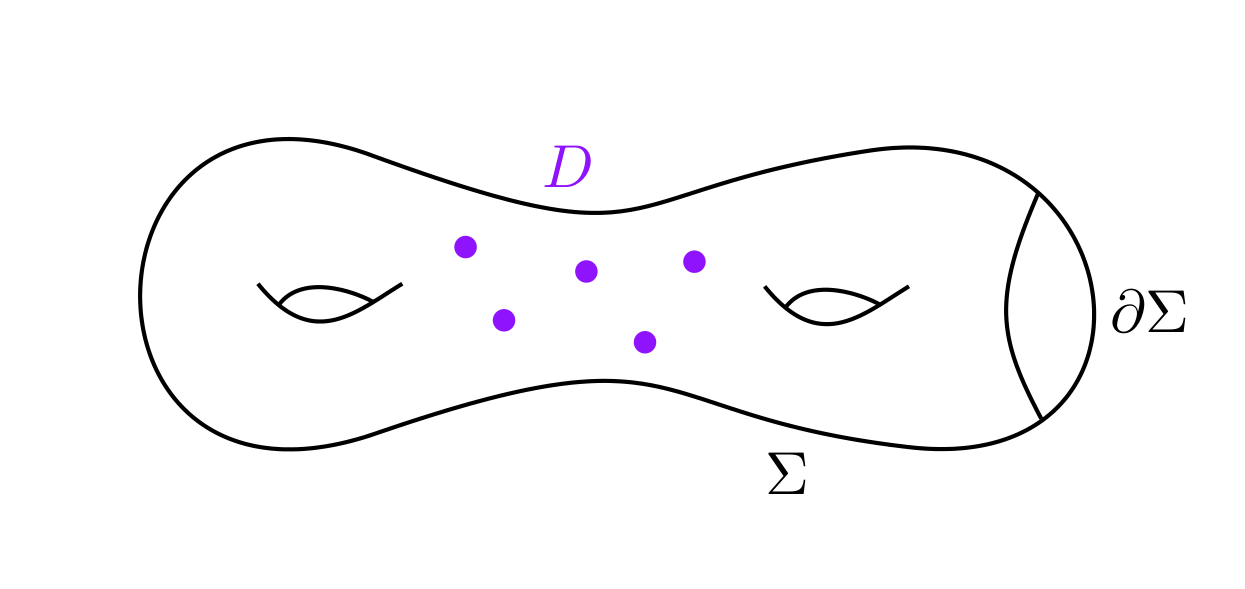
\includegraphics[width=0.50\linewidth]{fig_p097_1.png}
  \caption*{带边界与极点集的 Riemann 面（原文 PDF p.97 示意图，原文无编号）}
\end{figure}

设 $p\in D$，$z$ 是以 $p$ 为中心的局部坐标。则局部地 $\omega$ 可写成
\[
  \omega=\frac{\eta}{z^n},
\]
其中 $\eta$ 光滑，$n\in\mathbb{Z}$。由于极点阶数可以任意大，朴素的
$\int_\Sigma\omega$ 一般是发散的。解决这一发散问题的一种同调方法 [34] 如下。
我们可以把 $\omega$ 分解为
\[
  \omega=\alpha+\partial\beta,
\]
其中 $\alpha$ 是沿 $D$ 至多有\emph{对数极点}的 2-形式，$\beta$ 是沿 $D$ 有
\emph{任意阶极点}的 $(0,1)$-形式，而
$\partial=\dd z\frac{\partial}{\partial z}$ 是全纯 de Rham 微分。这样的分解
存在且不唯一。

\begin{wdefn}{10.8（[34]）}
  定义\textbf{正则化积分}
  \[
    \fint_\Sigma\omega:=\int_\Sigma\alpha+\int_{\partial\Sigma}\beta
  \]
  作为在 $\Sigma$ 上积分奇异形式 $\omega$ 的一种方案。
\end{wdefn}

它具有以下性质
% >>> p098
\begin{itemize}[leftmargin=1.6em,itemsep=0.2em]
  \item 它不依赖于 $\alpha,\beta$ 的选取；
  \item $\fint_\Sigma$ 在共形变换下不变；
  \item $\fint_\Sigma\partial(-)=\int_{\partial\Sigma}(-)$；
  \item $\fint_\Sigma\bar\partial(-)=\operatorname{Res}(-)$。
\end{itemize}

% [Tutor Note: 这四条性质刻画了 $\fint$ 与普通积分的差别：第三条是全纯 de Rham
% 微分的“Stokes 型”性质，第四条是 Dolbeault 微分给出留数——注意两条的右端分别是
% 边界积分与留数，方向/符号取决于 $\Sigma$ 的定向与 $D$ 的局部坐标选取，核对时
% 务必固定定向约定。$\alpha$ 允许对数极点、$\beta$ 允许任意阶极点，正是为了让
% $\fint$ 在共形变换下不变。]

正则化积分延拓了光滑形式的通常积分，即下述图表交换：
\begin{figure}[htbp]
  \centering
  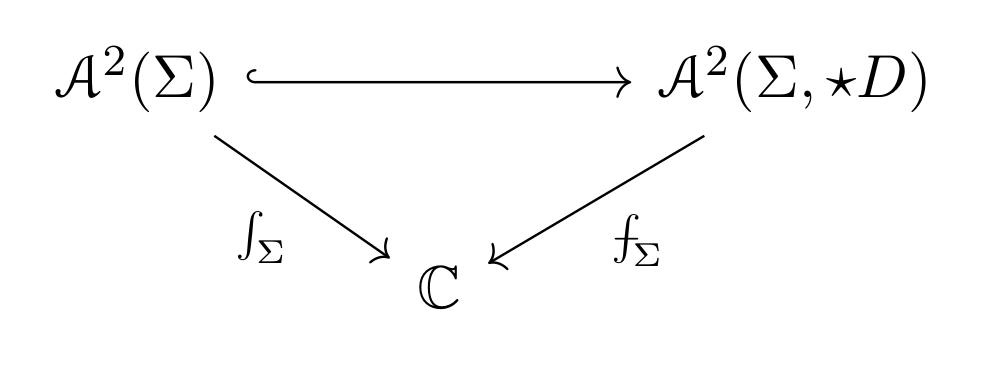
\includegraphics[width=0.40\linewidth]{fig_p098_1.png}
  \caption*{正则化积分与通常积分相容的交换图（原文 PDF p.98 示意图，原文无编号）}
\end{figure}

我们可以用它来定义 $\Sigma$ 的构型空间上的积分
\[
  \operatorname{Conf}_n(\Sigma)=\Sigma^n-\Delta
  =\left\{(p_1,\cdots,p_n)\in\Sigma^n\,\middle|\,p_i\neq p_i,\ \forall i\neq j\right\},
\]
并定义
\[
  \fint_{\Sigma^n}:\ \mathcal{A}^{2n}(\Sigma^n,\star\Delta)
  \longrightarrow\mathbb{C}
\]
为
\[
  \fint_{\Sigma^n}(-)=\fint_{\Sigma_1}\fint_{\Sigma_2}\cdots
  \fint_{\Sigma_n}(-).
\]
它不依赖于 $\Sigma^n$ 中各因子次序的选取；Fubini 型定理成立。这赋予了
$\fint_{\Sigma^n}\Omega$ 一个内蕴正则化的含义，其中 $\Omega$ 是 Feynman 图的
被积式。这就解释了为什么该理论是 UV 有限的。

% [Tutor Note: 原文构型空间定义中第二个条件写作 $p_i\neq p_i$，显然应为
% $p_i\neq p_j$（$i\neq j$），这是原书笔误；此处照录原式，请核对原书 p.97
% （PDF p.98）。另外 $\mathcal{A}^{2n}(\Sigma^n,\star\Delta)$ 表示在
% $\Sigma^n$ 的“对角邻域”上允许指定极点的形式空间，$\star\Delta$ 是奇性支撑的
% 记号（与 p.96 的 $\star D$ 同义）。]

\subsection{BV 量子化的同调方面（Homological Aspects of BV quantization）}

粗略地说，QFT 中的 BV 量子化导致：
\begin{itemize}[leftmargin=1.6em,itemsep=0.2em]
  \item 可观测量的因子化代数 $\Obs$ [11]，
  \item 由 $\Obs$ 的代数结构给出的链复形 $(C_\bullet(\Obs),d)$，
  \item 描述零模（在 $L=\infty$ 处）的 BV 代数 $(A,\Delta)$，带有 BV 积分映射
        \[
          \int_{BV}:\ A\longrightarrow\mathbb{C},
        \]
  \item 一个 $\mathbb{C}[[\hbar]]$-线性映射
        \[
          \langle-\rangle:\ C_\bullet(\Obs)\longrightarrow A((\hbar))
        \]
        它是从 $L=0$ 到 $L=\infty$ 的 HRG 流，满足 QME
        $(d+\hbar\Delta)\langle-\rangle=0$；QME 说的是 $\langle-\rangle$ 是
        交织 $d$ 与 $\hbar\Delta$ 的链映射，
  \item 导致指标定理的配分函数
        \[
          \operatorname{Index}=\int_{BV}\langle1\rangle.
        \]
\end{itemize}

回忆在 TQM 的例子中，我们有以下数据。
\begin{itemize}[leftmargin=1.6em,itemsep=0.2em]
  \item 因子化代数是 Weyl 代数：$\Obs=\mathcal{W}_{2n}$。
  \item 因子化复形是 Hochschild 链复形 $(C_\bullet(\Obs),d)$。
  \item 零模上的 BV 代数：
        $(A,\Delta)=(\Omega^\bullet(\mathbb{R}^{2n}),\mathcal{L}_{\omega^{-1}})$。
% >>> p099
  \item 自由关联映射
        \[
          \langle-\rangle:\ C_\bullet(\mathcal{W}_{2n})
          \longrightarrow\Omega^\bullet(\mathbb{R}^{2n})((\hbar)),
          \qquad b\mapsto\hbar\mathcal{L}_{\omega^{-1}}.
        \]
  \item 指标
        \[
          \operatorname{Index}=\int_{BV}\langle1\rangle
          =\left[\ee^{\omega_\hbar/\hbar}\widehat{A}\right].
        \]
\end{itemize}
在二维手征 QFT 的例子中，我们会有类似的故事 [23]。

% [Tutor Note: 这里 TQM 的指标公式写作 $\left[\ee^{\omega_\hbar/\hbar}\widehat{A}\right]$，
% 而第 9 章（PDF p.92）的对应公式是 $\int_X\ee^{-\omega_\hbar/\hbar}\widehat{A}(X)$，
% 两处指数差一个负号；疑为原文笔误或 $\omega_\hbar$ 的符号约定不同，请核对原书
% p.91 与 p.98（PDF p.92 与 p.99）。照录原文，不做改写。]

\subsection{手征链复形（Chiral Chain Complex）}

直观上，手征链复形可以看作 Hochschild 链复形的二维手征类比。
\begin{figure}[htbp]
  \centering
  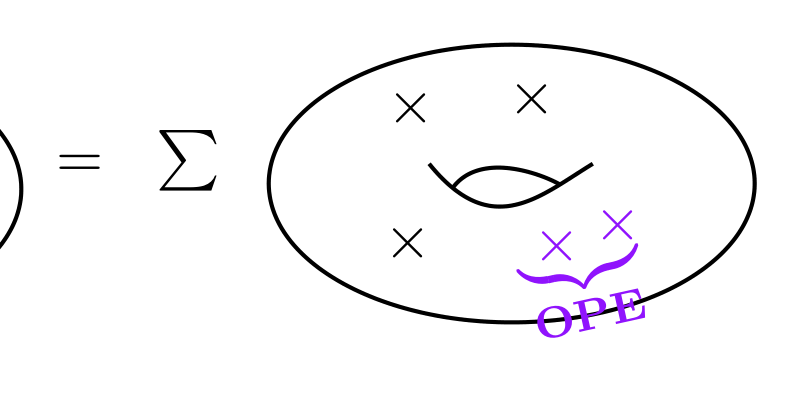
\includegraphics[width=0.33\linewidth]{fig_p099_1.png}
  \caption*{手征链复形微分的图形表示（原文 PDF p.99 示意图，原文无编号）}
\end{figure}

\begin{itemize}[leftmargin=1.6em,itemsep=0.2em]
  \item \textup{[41]} 研究了亏格 1 共形块的空间（即第 0 个椭圆手征同调）。
  \item \textup{[5]} 探讨了一般代数曲线的手征同调。
\end{itemize}

\paragraph*{Beilinson--Drinfeld 的构造（The construction of Beilinson--Drinfeld）}

给定以下数据：
\begin{itemize}[leftmargin=1.6em,itemsep=0.2em]
  \item $X=\Sigma$ 上右 $\mathcal{D}$-模的范畴 $\mathcal{M}(X)$，
  \item $X^S$ 上右 $\mathcal{D}$-模的范畴 $\mathcal{M}(X^S)$，使得每个元素
        $M\in\mathcal{M}(X^S)$ 是一个“收集”，对每个有限指标集 $I\in S$ 指定
        乘积 $X^I$ 上的右 $\mathcal{D}$-模 $M_{X^I}$，并满足一定的相容性条件，
  \item 存在一个正合、全忠实的嵌入
        \[
          \Delta_*^{(S)}:\ \mathcal{M}(X)\hookrightarrow\mathcal{M}(X^S),
        \]
        它经由对角映射 $\Delta^{(I)}:X\hookrightarrow X^I$ 得到，
  \item $\mathcal{M}(X^S)$ 带有（手征）张量结构 $\otimes^{\mathrm{ch}}$，
\end{itemize}
则手征代数 $\mathcal{A}$ 是通过 $\Delta_*^{(S)}$ 得到的一个 \textbf{Lie 代数对象}。

\begin{wrem}{10.9}
  手征代数 $\mathcal{A}$ 收集了所有“正规序算子”。
\end{wrem}

% [Tutor Note: 这段 Beilinson--Drinfeld 构造是全书最浓缩的一段，逐字读很容易迷失。
% 直观图像：$\mathcal{M}(X^S)$ 是“在所有有限多个点 $I\subset S$ 上同时取值的
% 右 $\mathcal{D}$-模”的范畴，$\Delta_*^{(S)}$ 把 $X$ 上的模沿对角嵌入拉回到
% $X^S$ 上；手征张量结构 $\otimes^{\mathrm{ch}}$ 只在互不相交的点之间可乘。手征
% 代数就是在这个对称张量范畴中的一个交换代数对象（原文称“Lie 代数对象”，指其
% 在 $\Delta_*^{(S)}$ 下的代数结构）。]

我们考虑 Chevalley--Eilenberg（CE）复形
\[
  (C(\mathcal{A}),d_{\mathrm{CE}})
  =\left(\bigoplus_{\bullet>0}\operatorname{Sym}^\bullet_{\otimes^{\mathrm{ch}}}
  \left(\Delta_*^{(S)}\mathcal{A}[1]\right),d_{\mathrm{CE}}\right).
\]
该复形的手征同调为
\[
  C^{\mathrm{ch}}(X,\mathcal{A})=R\Gamma_{DR}(X^S,C(\mathcal{A})).
\]
我们将聚焦于 $\beta\gamma$-$bc$ 系统，其中顶点算子代数（VOA）
$\mathcal{V}^{\beta\gamma-bc}$ 就是手征代数 $\mathcal{A}^{\beta\gamma-bc}$。

\begin{wthm}{10.10（[23]）}
  设 $E$ 是椭圆曲线。则 HRG 流给出一个映射
  \[
    \langle-\rangle_{2d}:\ C^{\mathrm{ch}}
    (E,\mathcal{A}^{\beta\gamma-bc})\longrightarrow\mathcal{A}((\hbar)),
  \]
  满足 QME $(d_{\mathrm{ch}}+\hbar\Delta)\langle-\rangle_{2d}=0$。粗略地说，
  $\langle-\rangle$ 由
  \[
    \langle\mathcal{O}_1\otimes\cdots\otimes\mathcal{O}_n\rangle_{2d}
    :=\fint_{E^n}\langle\mathcal{O}_1(z_1)\cdots\mathcal{O}_n(z_n)\rangle
  \]
  定义，其中 $\langle\mathcal{O}_1(z_1)\cdots\mathcal{O}_n(z_n)\rangle$ 是由
  Feynman 图给出的局部关联子，$\fint_{E^n}$ 是正则化积分。
\end{wthm}

% >>> p100
\subsection{2d $\to$ 1d 约化（2d $\to$ 1d reduction）}

我们把讨论总结如下。

\begin{center}
\begin{tabular}{ll}
\toprule
\textbf{一维 TQM} & \textbf{二维手征 QFT} \\
\midrule
结合代数 & 顶点/手征代数 \\
Hochschild 同调 & 手征同调 \\
QME $(\hbar\Delta+b)\langle-\rangle_{1d}=0$
  & QME $(\hbar\Delta+d_{\mathrm{ch}})\langle-\rangle_{2d}=0$ \\
$\langle\mathcal{O}_1\otimes\cdots\otimes\mathcal{O}_n\rangle_{1d}
  =\int_{\operatorname{Conf}_n(S^1)}$
  & $\langle\mathcal{O}_1\otimes\cdots\otimes\mathcal{O}_n\rangle_{2d}
  =\fint_{\Sigma^n}$ \\
\bottomrule
\end{tabular}
\end{center}

在物理中，椭圆曲线上的配分函数/关联函数由 $S^1$ 上的量子力学描述。

\begin{figure}[htbp]
  \centering
  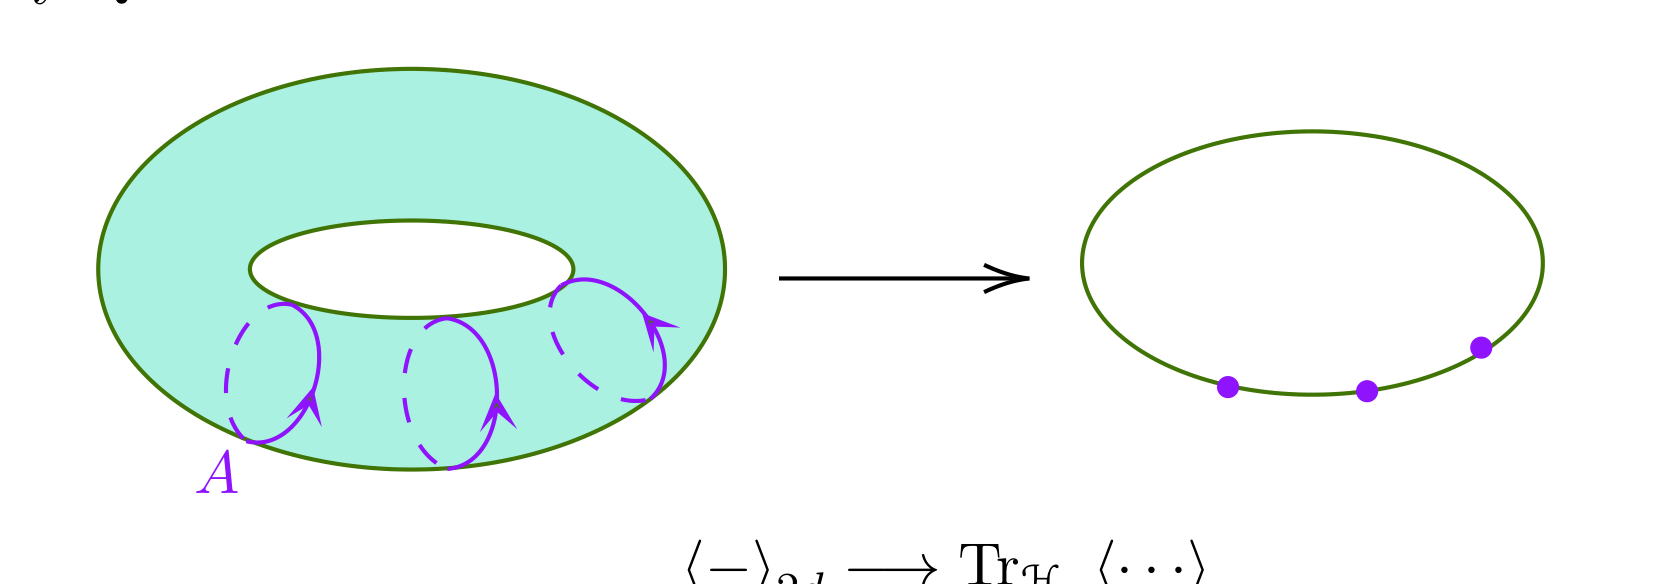
\includegraphics[width=0.67\linewidth]{fig_p100_1.png}
  \caption*{椭圆曲线上的关联函数约化为 $S^1$ 上的量子力学（原文 PDF p.100 示意图，原文无编号）}
\end{figure}
\[
  \langle-\rangle_{2d}\longrightarrow\operatorname{Tr}_{\mathcal{H}}
  \langle\cdots\rangle
\]

现在我们可以用正则化积分 $\fint_E$ 来定义二维关联函数。在一维情形，算子由
$A$-圈 $\oint_A$ 描述。这两个积分并不完全相同，而是通过\emph{全纯反常}相互关联。

\begin{wthm}{10.11（[34]）}
  设 $\Phi(z_1,\cdots,z_n;\tau)$ 是 $\mathbb{C}^n\times\mathbb{H}$ 上的亚纯椭圆
  函数，且在离开对角线处全纯。设 $A_1,\cdots,A_n$ 是椭圆曲线
  $E_\tau=\mathbb{C}/(\mathbb{Z}\oplus\tau\mathbb{Z})$ 上 $n$ 个互不相交的
  $A$-圈。

  \begin{figure}[htbp]
  \centering
  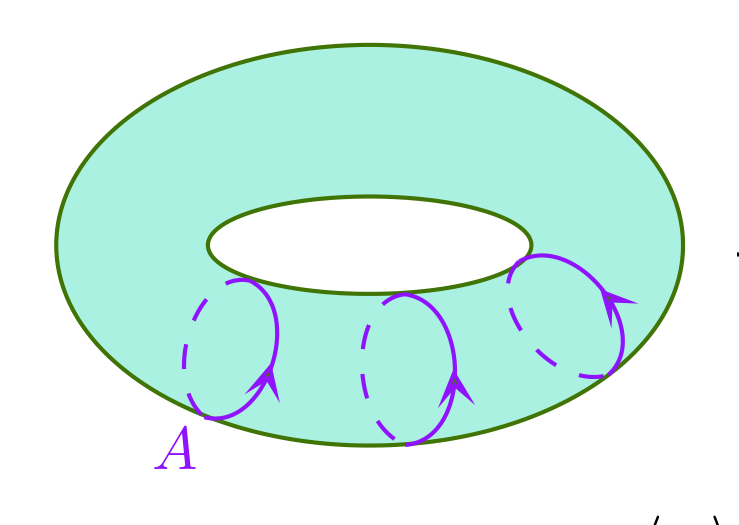
\includegraphics[width=0.30\linewidth]{fig_p100_2.png}
  \caption*{椭圆曲线 $E_\tau$ 上的互不相交 $A$-圈（原文 PDF p.100 示意图，原文无编号）}
\end{figure}

  则正则化积分
  \[
    \fint_{E_\tau^n}\left(\prod_{i=1}^n
    \frac{\dd^2z_i}{\operatorname{Im}\tau}\right)
    \Phi(z_1,\cdots,z_n;\tau)
  \]
  落在 $\mathcal{O}_{\mathbb{H}}\left[\frac{1}{\operatorname{Im}\tau}\right]$ 中。
  此外，我们有
  \[
    \lim_{\tau\to\infty}\fint_{E_\tau^n}\left(\prod_{i=1}^n
    \frac{\dd^2z_i}{\operatorname{Im}\tau}\right)\Phi
    =\frac{1}{n!}\sum_{\sigma\in S_n}\oint_{A_{\sigma(1)}}\dd z_1
    \cdots\oint_{A_{\sigma(n)}}\dd z_n\,\Phi,
  \]
  其中 $S_n$ 是 $n$ 个元素的置换群。本质地说，这意味着
  \[
    \fint_{E^n}\ \xrightarrow{\ \lim_{\tau\to\infty}\ }\
    \text{averaged}\oint_A,
  \]
  其中 $\fint_{E^n}$ 是几乎全纯模的，而平均化的 $\oint_A$ 是准模的。
\end{wthm}

% [Tutor Note: 定理 10.11 是“二维手征”与“一维 TQM”之间的桥梁：左边是二维椭圆
% 曲线上的正则化积分（几乎全纯模，依赖 $\tau,\bar\tau$），右边是 $A$-圈积分在
% 各置换下的平均（准模）。测度 $\prod_i\frac{\dd^2z_i}{\operatorname{Im}\tau}$
% 是环面上的平移不变测度（$\operatorname{Im}\tau$ 来自度规），极限 $\tau\to\infty$
% 使环面“拉长成 cylinder”，从而二维积分退化为沿 $A$-圈的积分平均。$\mathcal{O}_{\mathbb{H}}[\frac{1}{\operatorname{Im}\tau}]$
% 表示关于 $\tau$ 的全纯函数环添加 $\frac{1}{\operatorname{Im}\tau}$ 后得到的
% 几乎全纯函数环。]

% >>> p101
反全纯依赖有一个精确的描述。

\begin{wthm}{10.12（[35]）}
  设 $\Phi$ 是几乎椭圆函数。则
  \[
    \partial_Y\fint_{E_\tau^n}\Phi
    =\fint_{E_\tau^n}\partial_Y\Phi
    -\sum_{i<j}\fint_{E_\tau^{n-1}}
    \operatorname{Res}_{z_i=z_j}\left((z_i-z_j)\Phi\right).
  \]
\end{wthm}

这里 $Y=\frac{1}{\operatorname{Im}\tau}$。这给出\textbf{全纯反常方程}。

% [Tutor Note: 全纯反常方程把“对 $\bar\tau$（等价地 $Y=\frac{1}{\operatorname{Im}\tau}$）
% 的导数”与“二维正则化积分的边界/留数项”联系起来：右边第二项是当两点 $z_i\to z_j$
% 时在对角线上取留数所得的“碰撞项”，即积分区域边界的贡献。$Y=\frac{1}{\operatorname{Im}\tau}$
% 的约定与 $\tau=\tau_1+i\tau_2$、$\operatorname{Im}\tau=\tau_2$ 一致；若采用
% $\bar\tau$ 的另一种归一化，系数可能相差常数，核对时以原书 p.100（PDF p.101）
% 的 $Y$ 定义为准。]


% ---------- part14.tex ----------
% ============================================================
%  part14.tex  |  原文 PDF p.101–103（参考文献）
%  内容：References [1]–[41]（条目照录原文，不译；仅统一标点为 LaTeX 形式）
% ============================================================

\clearpage
\section*{参考文献（References）}
\addcontentsline{toc}{section}{参考文献（References）}

% [Tutor Note: 参考文献条目按学术惯例保留英文原貌，不作翻译。原文 PDF 的参考文献
% 存在若干明显的排印缺失，例如 [21] 的 "BatalinVilkovisky"（应为
% Batalin--Vilkovisky）、[34] 的 "14031474"（应为 1403--1474）、[35] 的
% "613645"（应为 613--645），这些在 PDF 版面图上即如此，属原文排版缺字；
% 本译本照录原文，读者引用时请以原出版物为准。]

\begingroup
\small
% >>> p101
\begin{enumerate}[label={[\arabic*]},leftmargin=2.8em,itemsep=0.18em,topsep=0.4em]
  \item Alexandrov, M., Schwarz, A., Zaboronsky, O., Kontsevich, M.
        \textit{The geometry of the master equation and topological quantum field
        theory}. International Journal of Modern Physics A, 12.07.(1997), 1405--1429.
  \item Axelrod, S. and Singer, I.M., \textit{Chern--Simons Perturbation Theory II}.
        J. Differ. Geom. 39 (hepth/9304087), 173213 (1993)
  \item Batalin, I. and Vilkovisky, G., \textit{Gauge algebra and quantization},
        Physics Letters B \textbf{102}(1), 27--31 (1981).
  \item Bayen, F., Flato, M., Fronsdal, C., Lichnerowicz, A., and Sternheimer, D.,
        \textit{Deformation theory and quantization. I. Deformations of symplectic
        structures}. Annals of Physics 111, no. 1 (1978): 61--110.
        \textit{Deformation theory and quantization. II. Physical applications}.
        Annals of Physics 111, no. 1 (1978): 111--151.
  \item Beilinson, A., and Drinfeld, V., \textit{Chiral algebras}, volume 51,
        American Mathematical Soc., 2004.
  \item Berezin, F.. \textit{Feynman path integrals in a phase space}. Soviet
        Physics Uspekhi 23.11 (1980): 763.
  \item Bordemann, M., \textit{Deformation quantization: a survey}. Journal of
        Physics: Conference Series. Vol. 103. No. 1. IOP Publishing, 2008.
  \item Bressler, P., Nest, R., and Tsygan, B., \textit{Riemann--Roch Theorems via
        Deformation Quantization, I}, Advances in Mathematics 167(1), 1--25 (2002).
  \item Cattaneo, A.S., and Felder, G.. \textit{Poisson sigma models and deformation
        quantization}. Modern Physics Letters A 16.04n06 (2001): 179--189.
  \item Coleman, S.. \textit{Aspects of symmetry: selected Erice lectures}.
        Cambridge University Press, 1988.
  \item Costello, K. and Gwilliam, O., \textit{Factorization algebras in quantum
        field theory}, Vol 1, 2. Cambridge University Press, 2021.
  \item Costello, K., \textit{Renormalization and effective field theory}, volume 170
        of \textit{Mathematical Surveys and Monographs}, American Mathematical Soc., 2011.
  \item De Wilde, M. and Lecomte, P., \textit{Existence of star-products and of
        formal deformations of the Poisson Lie algebra of arbitrary symplectic
        manifolds}. Letters in Mathematical Physics 7 (1983): 487--496.
  \item Dijkgraaf, R. and Witten, E., \textit{Topological gauge theories and group
        cohomology}. Communications in Mathematical Physics 129 (1990): 393--429.
  \item Feynman, R., Hibbs, A. and Styer, D., \textit{Quantum mechanics and path
        integrals}. Courier Corporation, 2010.
  \item Feynman, R. and Brown, L., \textit{Feynman's thesis: a new approach to
        quantum theory}. World Scientific, 2005.
  % >>> p102
  \item Fedosov, B., \textit{A simple geometrical construction of deformation
        quantization}. Journal of differential geometry 40.2 (1994): 213--238.
  \item Fedosov, B., \textit{Deformation quantization and index theory}.
        Mathematical topics 9 (1996).
  \item Feigin, B., Felder, G. and Shoikhet, B., \textit{Hochschild cohomology of the
        Weyl algebra and traces in deformation quantization}. Duke Mathematical
        Journal 127 (3) 487--517, (2005)
  \item Feigin, B. and Tsygan, B., \textit{Riemann--Roch theorem and Lie algebra
        cohomology}, in \textit{Proceedings of the Winter School "Geometry and
        Physics"}, pages 15--52, Circolo Matematico di Palermo, 1989.
  \item Grady, R., Li, Q. and Li, S.. \textit{BatalinVilkovisky quantization and the
        algebraic index}. Advances in Mathematics 317 (2017): 575--639.
  \item Ginzburg, V., \textit{Lectures on noncommutative geometry}.
        arXiv:math/0506603 (2005).
  \item Gui, Z. and Li, S., \textit{Elliptic Trace Map on Chiral Algebras},
        (12 2021), arXiv: 2112.14572.
  \item Gui, Z., Li. S., and Xu, K., \textit{Geometry of localized effective theories,
        exact semiclassical approximation and the algebraic index}. Communications
        in Mathematical Physics 382.1 (2021): 441--483.
  \item Kontsevich, M., \textit{Feynman diagrams and low-dimensional topology}.
        First European Congress of Mathematics Paris, July 610, 1992: Vol. II:
        Invited Lectures (Part 2). Basel: Birkhäuser Basel, 1994.
  \item Kontsevich, M, \textit{Deformation quantization of Poisson manifolds}.
        Letters in Mathematical Physics 66 (2003): 157--216.
  \item Lada, T. and Stasheff, J., \textit{The resurgence of $L_{\infty}$-structures
        in field theory}, Differ. Geom. Appl. \textbf{77}, 101755 (2021).
  \item Li, S., \textit{Feynman graph integrals and almost modular forms}, Comm. in
        Number Theory and Physics, 6, 2012.
  \item Li, S., \textit{Vertex algebras and quantum master equation}. J.Diff.Geom.
        123 (2023), no 3, 461--521.
  \item Li, S., \textit{Classical Mechanics and Geometry}. Boston, MA: International
        Press of Boston, 2023.
  \item Li, S., \textit{Electromagnetism and Geometry}. Boston, MA: International
        Press of Boston, 2023.
  \item Li, S., Wang, Z., Yang, P., \textit{Stochastic Calculus and Hochschild
        Homology}, arXiv:2501.12360 [math.PR]
  \item Li, S., and Zeng, K., \textit{Homotopy algebras in higher spin theory},
        Adv. Theor. Math. Phys. \textbf{24}(3), 757--819 (2020)
  \item Li, S., Zhou, J., \textit{Regularized Integrals on Riemann Surfaces and
        Modular Forms}. Commun. Math. Phys. 388, 14031474 (2021).
  \item Li, S., Zhou, J., \textit{Regularized Integrals on Elliptic Curves and
        Holomorphic Anomaly Equations}. Commun. Math. Phys. 401, pp 613645 (2023).
  \item Loday, J., \textit{Cyclic homology}. Vol. 301. Springer Science \& Business
        Media, 2013.
  \item Nest, R., and Tsygan, B., \textit{Algebraic index theorem}. Communications
        in Mathematical Physics 172, 223--262 (1995)
  % >>> p103
  \item Tsygan, B., \textit{Cyclic homology}. \textit{Cyclic homology in
        non-commutative geometry}. Vol. 121, 73--113. Springer Science \& Business
        Media (2003)
  \item Wang, M., \textit{Feynman Graph Integrals on $\C^d$}. Commun. Math. Phys.
        406.5 (2025): 116.
  \item Witten, E., \textit{Analytic continuation of Chern--Simons theory}. AMS/IP
        Stud. Adv. Math 50 (2011): 347.
  \item Zhu, Y., \textit{Global vertex operators on Riemann surfaces}, Commun. Math.
        Phys. \textbf{165}(3), 485--531 (1994).
\end{enumerate}
\endgroup

\end{document}
